\documentclass[a4paper,11pt,twoside]{memoir}
\chapterstyle{veelo}

\usepackage{TUINFDA}

\usepackage{placeins}
\usepackage{amsmath}
\usepackage{epsfig}
\usepackage{url}
\usepackage{hyperref}					% links in pdf
\usepackage{graphicx}            			% Figures
\usepackage{verbatim}            			% Code-Environment
%\usepackage[lined,linesnumbered,algochapter]{algorithm2e} % Algorithm-Environment
\usepackage{multirow}
\usepackage[linesnumbered,ruled,vlined]{algorithm2e}

\usepackage{pgf}					
\usepackage{tikz}					% tikz graphics
\usetikzlibrary{arrows,automata}

\usepackage{ngerman}
\usepackage[ngerman]{babel}
\usepackage{bibgerm,cite}       % Deutsche Bezeichnungen, Automatisches Zusammenfassen von Literaturstellen
\usepackage[ngerman]{varioref}  % Querverweise
\usepackage{rotating}
% to use the german charset include cp850 for MS-DOS, ansinew for Windows and latin1 for Linux.
% \usepackage[latin1]{inputenc}

\thesistitle{A Hybrid Algorithm for the Partition Coloring Problem}
\thesissubtitle{Optional Subtitle} % optional
\thesisdate{21.Oct.2013}

% all titles and designations have to be gender-related!
\thesisdegree{Diplom-Ingenieurin}{Diplom-Ingenieurin}
\thesiscurriculum{Computational Intelligence}{Computational Intelligence} % your study
\thesisverfassung{Verfasserin} % Verfasser
\thesisauthor{Gilbert Fritz} % your name
\thesisauthoraddress{Schlosshofer Straße 49/18} % your address
\thesismatrikelno{0827276} % your registration number

\thesisbetreins{Univ.Ass. Dipl.-Ing. Dr.techn. Dr. Bin Hu}
\thesisbetrzwei{Univ.-Prof. Dipl.-Ing. Dr.techn. Günther Raidl}
%\thesisbetrdrei{Dr. Vorname Familienname} % optional

% define page numbering styles
\makepagestyle{numberCorner}
\makeevenfoot{numberCorner}{\thepage}{}{}
\makeoddfoot{numberCorner}{}{}{\thepage}

% define custom macros for specific formats or names
\newcommand{\uml}[1]{\texttt{#1}}
\newcommand{\cd}{\textsf{Class Diagram}}

\begin{document}

\captionnamefont{\bfseries}

%%%%%%%%%%%%%%%%%%%%%%%%%%%%%%%%%%%%%%%%%
%%%   FRONTMATTER    %%%%%%%%%%%%%%%%%%%%
%%%%%%%%%%%%%%%%%%%%%%%%%%%%%%%%%%%%%%%%%
\frontmatter
\pagenumbering{roman}

%%%%%%%%%%%%%%%%%%%%%%%%%%%%%%%%%%%%%%%%%
%%%   TITLEPAGES    %%%%%%%%%%%%%%%%%%%%%
%%%%%%%%%%%%%%%%%%%%%%%%%%%%%%%%%%%%%%%%%

% the german title page is required as first page
% $Id: titlepage.tex 1752 2010-03-20 11:07:02Z tkren $
%
% TU Wien - Faculty of Informatics
% thesis titlepage
%
% This titlepage is using the geometry package, see
% <http://www.ctan.org/macros/latex/contrib/geometry/geometry.pdf>
%
% For questions and comments send an email to
% Thomas Krennwallner <tkren@kr.tuwien.ac.at>
% or to Petra Brosch <brosch@big.tuwien.ac.at>
%

\selectlanguage{ngerman}

% setup page dimensions for titlepage
\newgeometry{left=2.4cm,right=2.4cm,bottom=2.5cm,top=2cm}

% force baselineskip and parindent
\newlength{\tmpbaselineskip}
\setlength{\tmpbaselineskip}{\baselineskip}
\setlength{\baselineskip}{13.6pt}
\newlength{\tmpparindent}
\setlength{\tmpparindent}{\parindent}
\setlength{\parindent}{17pt}

% first titlepage
\thispagestyle{tuinftitlepage}

%
% Kludge: for each titlepage set \pagenumbering to a different
% style. This is used to fix a problem with hyperref, because there
% are multiple "page 1" and hyperref hates that
%
\pagenumbering{Alph}

\begin{center}
{\ \vspace{3.4cm}}

\begin{minipage}[t][2.8cm][s]{\textwidth}%
\centering
\thesistitlefontHUGE\sffamily\bfseries\tuinfthesistitle\\
\bigskip
{\thesistitlefonthuge\sffamily\bfseries\tuinfthesissubtitle}
\end{minipage}

\vspace{1.3cm}

{\thesistitlefontLARGE\sffamily \tuinfthesistype}

\vspace{6mm}

{\thesistitlefontlarge\sffamily zur Erlangung des akademischen Grades}

\vspace{6mm}

{\thesistitlefontLARGE\sffamily\bfseries \tuinfthesisdegree}

\vspace{6mm}

{\thesistitlefontlarge\sffamily im Rahmen des Studiums}

\vspace{6mm}

{\thesistitlefontLarge\sffamily\bfseries \tuinfthesiscurriculum}

\vspace{6.5mm}

{\thesistitlefontlarge\sffamily eingereicht von}

\vspace{6mm}

{\thesistitlefontLarge\sffamily\bfseries \tuinfthesisauthor}

\vspace{1.5mm}

{\thesistitlefontlarge\sffamily Matrikelnummer \tuinfthesismatrikelno} 

\vspace{1.4cm}

\vspace{0pt}\raggedright\thesistitlefontnormalsize\sffamily
\begin{minipage}[t][1.6cm][t]{\textwidth}%
  %
  an der

  Fakult\"{a}t f\"{u}r Informatik der Technischen Universit\"{a}t Wien
\end{minipage}

\begin{minipage}[t][4cm][t]{\textwidth}%
  \vspace{0pt}\raggedright\thesistitlefontnormalsize\sffamily
  %
  \begin{tabbing}%
	    \hspace{19mm} \= \hspace{66mm} \kill
	    \tuinfthesisbetreuung: \> \tuinfthesisbetreins\\
	    Mitwirkung: \> \tuinfthesisbetrzwei\\
	                \> \tuinfthesisbetrdrei
  \end{tabbing}
\end{minipage}

\begin{minipage}[t][1.5cm][t]{\textwidth}%
  \vspace{0pt}\sffamily\thesistitlefontnormalsize
  \begin{tabbing}%
    \hspace{45mm} \= \hspace{63mm} \= \hspace{51mm} \kill
    Wien, \tuinfthesisdate \> {\raggedright\rule{51mm}{0.5pt}} \> {\raggedright\rule{51mm}{0.5pt}} \\
    \> \begin{minipage}[t][0.5cm][t]{51mm}\centering (Unterschrift \tuinfthesisverfassung)\end{minipage}
    \> \begin{minipage}[t][0.5cm][t]{51mm}\centering (Unterschrift \tuinfthesisbetreuung)\end{minipage}
    \end{tabbing}
\end{minipage}

\end{center}

% we want an empty page right after first titlepage
\pagestyle{empty}
\cleardoublepage

% we're done with the titlepages, proceed with default pagenumbering
\pagenumbering{roman}

% restore baselineskip
\setlength{\baselineskip}{\tmpbaselineskip}
\setlength{\parindent}{\tmpparindent}

% back to normal geometry
\restoregeometry

\selectlanguage{english}

%%% Local Variables:
%%% TeX-PDF-mode: t
%%% TeX-debug-bad-boxes: t
%%% TeX-parse-self: t
%%% TeX-auto-save: t
%%% reftex-plug-into-AUCTeX: t
%%% End:


% an english translation may follow
% $Id: titlepage.tex 1752 2010-03-20 11:07:02Z tkren $
%
% TU Wien - Faculty of Informatics
% thesis titlepage
%
% This titlepage is using the geometry package, see
% <http://www.ctan.org/macros/latex/contrib/geometry/geometry.pdf>
%
% For questions and comments send an email to
% Thomas Krennwallner <tkren@kr.tuwien.ac.at>
% or to Petra Brosch <brosch@big.tuwien.ac.at>
%

% setup page dimensions for titlepage
\newgeometry{left=2.4cm,right=2.4cm,bottom=2.5cm,top=2cm}

% force baselineskip and parindent
%\newlength{\tmpbaselineskip}
%\setlength{\tmpbaselineskip}{\baselineskip}
%\setlength{\baselineskip}{13.6pt}
%\newlength{\tmpparindent}
%\setlength{\tmpparindent}{\parindent}
%\setlength{\parindent}{17pt}

% first titlepage
\thispagestyle{tuinftitlepage}

%
% Kludge: for each titlepage set \pagenumbering to a different
% style. This is used to fix a problem with hyperref, because there
% are multiple "page 1" and hyperref hates that
%
\pagenumbering{Roman}

\begin{center}
{\ \vspace{3.4cm}}

\begin{minipage}[t][2.8cm][s]{\textwidth}%
\centering
\thesistitlefontHUGE\sffamily\bfseries\tuinfthesistitle\\
\bigskip
{\thesistitlefonthuge\sffamily\bfseries\tuinfthesissubtitle}
\end{minipage}

\vspace{1.3cm}

{\thesistitlefontLARGE\sffamily \tuinfthesistypeen}

\vspace{6mm}

{\thesistitlefontlarge\sffamily submitted in partial fulfillment of the requirements for the degree of}

\vspace{6mm}

{\thesistitlefontLARGE\sffamily\bfseries \tuinfthesisdegreeen}

\vspace{6mm}

{\thesistitlefontlarge\sffamily in}

\vspace{6mm}

{\thesistitlefontLarge\sffamily\bfseries \tuinfthesiscurriculumen}

\vspace{6.5mm}

{\thesistitlefontlarge\sffamily by}

\vspace{6mm}

{\thesistitlefontLarge\sffamily\bfseries \tuinfthesisauthor}

\vspace{1.5mm}

{\thesistitlefontlarge\sffamily Registration Number \tuinfthesismatrikelno} 

\vspace{1.4cm}

\begin{minipage}[t][1.6cm][t]{\textwidth}%
  \vspace{0pt}\raggedright\thesistitlefontnormalsize\sffamily
  %
  to the Faculty of Informatics 

  at the Vienna University of Technology
\end{minipage}

\vspace{0pt}\raggedright\thesistitlefontnormalsize\sffamily
\begin{minipage}[t][4cm][t]{\textwidth}%
  \begin{tabbing}%
	    \hspace{19mm} \= \hspace{66mm} \kill
	    Advisor: \> \tuinfthesisbetreins\\
	    Assistance: \> \tuinfthesisbetrzwei\\
	                \> \tuinfthesisbetrdrei
     \end{tabbing}
\end{minipage}

\begin{minipage}[t][1.5cm][t]{\textwidth}%
  \vspace{0pt}\sffamily\thesistitlefontnormalsize
  \begin{tabbing}%
    \hspace{45mm} \= \hspace{63mm} \= \hspace{51mm} \kill
    Vienna, \tuinfthesisdate \> {\raggedright\rule{51mm}{0.5pt}} \> {\raggedright\rule{51mm}{0.5pt}} \\
    \> \begin{minipage}[t][0.5cm][t]{51mm}\centering (Signature of Author)\end{minipage}
    \> \begin{minipage}[t][0.5cm][t]{51mm}\centering (Signature of Advisor)\end{minipage}
    \end{tabbing}
\end{minipage}

\end{center}

% we want an empty page right after first titlepage
\pagestyle{empty}
\cleardoublepage

% we're done with the titlepages, proceed with default pagenumbering
\pagenumbering{roman}

% restore baselineskip
\setlength{\baselineskip}{\tmpbaselineskip}
\setlength{\parindent}{\tmpparindent}

% back to normal geometry
\restoregeometry


%%% Local Variables:
%%% TeX-PDF-mode: t
%%% TeX-debug-bad-boxes: t
%%% TeX-parse-self: t
%%% TeX-auto-save: t
%%% reftex-plug-into-AUCTeX: t
%%% End:
 % optional

%%%%%%%%%%%%%%%%%%%%%%%%%%%%%%%%%%%%%%%%%
%%%   ERKLAERUNG DER SELBSTAENDIGKEIT   %
%%%%%%%%%%%%%%%%%%%%%%%%%%%%%%%%%%%%%%%%%
\cleardoublepage
\selectlanguage{ngerman}
\chapter*{Erklärung zur Verfassung der Arbeit}

\tuinfthesisauthor\\
\tuinfthesisauthoraddress

\vspace*{1.2cm}

Hiermit erkläre ich, dass ich diese Arbeit selbständig verfasst habe, 
dass ich die verwendeten Quellen und Hilfsmittel vollständig angegeben 
habe und dass ich die Stellen der Arbeit - einschließlich Tabellen, 
Karten und Abbildungen -, die anderen Werken oder dem Internet im 
Wortlaut oder dem Sinn nach entnommen sind, auf jeden Fall unter Angabe 
der Quelle als Entlehnung kenntlich gemacht habe.\\

\vspace*{2cm}
\begin{tabbing}%
    \hspace{58mm} \= \hspace{28mm} \= \hspace{58mm} \kill
    {\raggedright\rule{58mm}{0.5pt}} \> \> {\raggedright\rule{58mm}{0.5pt}} \\
    \begin{minipage}[t][0.5cm][t]{58mm}
	\vspace{0pt}\sffamily\thesistitlefontnormalsize
	\centering (Ort, Datum)
    \end{minipage}
    \> \>
    \begin{minipage}[t][0.5cm][t]{58mm}
	\vspace{0pt}\sffamily\thesistitlefontnormalsize
	\centering (Unterschrift \tuinfthesisverfassung)
    \end{minipage}
\end{tabbing}


\selectlanguage{english}

%%%%%%%%%%%%%%%%%%%%%%%%%%%%%%%%%%%%%%%%%
%%%   ACKNOWLEDGEMENTS    %%%%%%%%%%%%%%%
%%%%%%%%%%%%%%%%%%%%%%%%%%%%%%%%%%%%%%%%%

% optional acknowledgements may be included in german or in english
\chapter*{Danksagung}

Ich danke meinen Betreuern, ao. Univ.-Prof. Dipl.-Ing. Dr.techn. Günther Raidl und Univ.Ass. Dipl.-Ing. Dr.techn. Bin Hu für ihre Unterstützung bei der Erstellung dieser Arbeit durch ihr konstruktives Feedback und ihre Ideen, welche es mir ermöglicht haben, immer neue Aspekte der Problemstellung zu erkennen.\\

Besonderer Dank gilt meinen Eltern, Franz und Justine Fritz, sowie meinem Bruder Wolfi, der mein Interesse an Computern früh gefördert hat. Weiters möchte ich meinem Studienkollegen Philipp Gebhard danken, dessen Begeisterung an theoretischeren Themen der Informatik mich anzustecken vermochte. Auch meiner Partnerin Odnoo danke ich für ihre Unterstützung. 		% optional
\chapter*{Acknowledgements}

Optional acknowledgements may be inserted here.	% optional

%%%%%%%%%%%%%%%%%%%%%%%%%%%%%%%%%%%%%%%%%
%%%   ABSTARCT    %%%%%%%%%%%%%%%%%%%%%%%
%%%%%%%%%%%%%%%%%%%%%%%%%%%%%%%%%%%%%%%%%

\chapter*{Abstract}

Todo
\cleardoublepage
\selectlanguage{ngerman}
\chapter*{Kurzfassung}

Das Partition Coloring Problem (PCP) generalisiert das Vertex Coloring Problem (VCP) durch Unterteilung der Knotenmenge in Gruppen und besteht aus der Berechnung einer Knotenfärbung des durch Selektion genau eines Knotens pro Gruppe induzierten Subgraphens. Das PCP gehört zur Gruppe der so genannten $\mathit{NP}$-schweren Probleme, i.e. Probleme für die kein effizientes Verfahren zur Findung einer exakten Lösung besteht. Eine seiner Anwendungen besteht in der Zuordnung von Wellenlängen zu Datenübertragungsleitungen optischer Computernetzwerke, wie sie heute beispielsweise als Backbone in der Infrastruktur des Internets vorkommen. Im Gegensatz zum VCP bleibt das PCP bis heute wenig erforscht.\\

Diese Arbeit präsentiert ein metaheuristisches Verfahren \textit{Hybrid-PCP} zur Lösung des PCP, dass sich zusätzlich exakter Methoden bedient um Teilprobleme zu lösen. Dabei wird eine Verbesserungsstrategie verfolgt, in der Knoten in spezifischen Teilgraphen neu selektiert und eingefärbt werden, wobei temporär auch ungültige Lösungen zugelassen werden. Die Gültigkeit wird danach mittels Tabusuche wiederhergestellt. Die Hauptinnovation dieser Arbeit liegt im Aufwand, der für die Neuselektion und -einfärbung der Teilgraphen aufgewendet wird, als dass dafür eine Heuristik und zwei mathematische Programmformulierungen eingesetzt werden. Der Algorithmus wird mit unterschiedlicher Parametrisierung als auch leichten Variationen evaluiert, die Ergebnisse miteinander und mit solcher vorhergehender Arbeiten verglichen. Weitere Experimente werden mit der Erstellung initialer Lösungen durchgeführt, wobei zwei bereits bekannte Algorithmen \textit{OneStepCD} und eine Adaption des für VCP entwickelten \textit{DANGER} Algorithmus miteinander verglichen werden. \textit{Hybrid-PCP} kann betreffend Lösungsqualität und Laufzeit mit den besten bisher gefundener Lösungsansätze konkurrieren. Der Autor legt weiters eine Reflexion des Verfahrens sowie einen Verbesserungsvorschlag dar.

\selectlanguage{english}

%%%%%%%%%%%%%%%%%%%%%%%%%%%%%%%%%%%%%%%%%
%%%   CONTENTS    %%%%%%%%%%%%%%%%%%%%%%%
%%%%%%%%%%%%%%%%%%%%%%%%%%%%%%%%%%%%%%%%%
% uncomment to set document language to german (results in "Inhaltsverzeichnis", "Kapitel", "Abbildung", etc. instead of "Contents", "Chapter", and "Figure"), otherwise the document's language is english
%\selectlanguage{ngerman}

\setcounter{tocdepth}{1}

\cleardoublepage
\pagestyle{numberCorner}
\tableofcontents*

%%%%%%%%%%%%%%%%%%%%%%%%%%%%%%%%%%%%%%%%%
%%%   MAINMATTER    %%%%%%%%%%%%%%%%%%%%%
%%%%%%%%%%%%%%%%%%%%%%%%%%%%%%%%%%%%%%%%%

\mainmatter
\pagenumbering{arabic}
\pagestyle{numberCorner}

%%%%%%%%%%%%%%%%%%%%%%%%%%%%%%%%%%%%%%%%%
\chapter{Introduction}
\label{ch:intro}
%%%%%%%%%%%%%%%%%%%%%%%%%%%%%%%%%%%%%%%%%
\section{Motivation}

In order to obey the emerging demand for advanced broadband Internet applications such as video-conferences, high performance computing and others, extensive networks capacities have to be achieved. Links in optical networks operate much faster than their currently available electronic counterparts. Combined with the technique of Wavelength Division Multiplexing (WDM), which permits the simultaneous transmission of different channels along the same fiber \cite{noronha-06}, these so called Wavelength Routed Optical Networks (WRON's) are promising candidates for providing a flexible transport backbone network \cite{krishnaswamy-01}. They bring out new problems in coordination of wavelengths usage \cite{murthy-02}. One of them is the Routing and Wavelength Assignment Problem (RWA), which consists in routing a set of light-paths and assigning a wavelength to each of them. The variant where all connection requirements are known beforehands and which aims to minimize the amount of used wavelength is called min-RWA and found to be $\mathcal{NP}$-hard \cite{erlebach-01}.\\\\
Assigning wavelengths to one out of many paths for each connection requirement is equivalent to the $\mathcal{NP}$-hard \textbf{Partition Coloring Problem (PCP)} \cite{li-00}, also known as \textbf{Partition Graph Coloring Problem (PGCP)} which is subject of this thesis. Given a graph consisting of a clustered set of vertices and a set of edges, the aim is to select one vertex per cluster and for each vertex in the resulting subgraph assign a color in the way that the overall number of colors -- which in this context is said to be the chromatic number -- is minimized. If each cluster holds only one vertex, the problem reduces to the Standard Vertex Coloring Problem (VCP), which is used for a wide range of applications as scheduling, register allocation, pattern matching and others and has been studied extensively. In contrast, only a few papers have been published on PCP so far.\\\\
The aim of this thesis is to explore a solution method that has not been subject of publications on PCP yet,	in order to achieve advanced approximization methods.
%Because of its complexity, the PCP counts to the class of $\mathcal{NP}$-optimization problems (NPO)


\section{Guide to the Thesis}

Definitions from graph theory and basic concepts which are required for the analysis of the Partition Coloring Problem are introduced in Chapter \ref{ch:prelim}.Afterwards, Chapter \ref{ch:problem} defines the PCP as well as the min-RWA formally and comments their computational complexity. Previous works and related research done so far is presented in Chapter \ref{ch:previous}. Chapter \ref{ch:approach} provides details of the approach developed for the PCP and Chapter \ref{ch:results} presents its experimental results. Chapter \ref{ch:summary} summarizes the knowledge achieved within this thesis, brings the considered approach into question and finally proposes a possible further work.

%%%%%%%%%%%%%%%%%%%%%%%%%%%%%%%%%%%%%%%%%
\chapter{Preliminaries}
\label{ch:prelim}
%%%%%%%%%%%%%%%%%%%%%%%%%%%%%%%%%%%%%%%%%
\section{Graph Theory Definitions}



\section{Metaheuristics}




%%%%%%%%%%%%%%%%%%%%%%%%%%%%%%%%%%%%%%%%%
\chapter{Problem Definition}
\label{ch:problem}
%%%%%%%%%%%%%%%%%%%%%%%%%%%%%%%%%%%%%%%%%
\section{Partition Coloring Problem}

%2.6
%10
%Generalization of Network Design Problems
%Several Network Design Problems can be generalized by partitioning the node set V into
%clusters Vk , k ∈ K [5]. Even if those clusters are not necessarily disjunct, the proposed
%algorithms in this thesis requires node disjunct clusters (i. e. Vi ∩ Vj = ∅, ∀i, j ∈ K, i = j).
%A common distinction between three different types (exactly, at least, at most) of such
%generalizations can be done with respect to the number of nodes that need to be in a feasible
%solution of the problem.
%A feasible solution of an exactly generalized problem selects exactly one vertex from each
%cluster Vk (∀k = 1, . . . , r). Similar to that, the at least version requires the solution to
%contain at least one node from each cluster and the at most version requires the solution to
%contain at most one node from each cluster.
%Typically the prefixes E-, L-, and M- are used to distinguish between the different
%generalization types of the same problem (i. e. L-GMST stands for the at least version,
%E-GMST for the exact version, and M-GMST for the at most version of the GMST problem).
%A missing prefix usually refers to the exact generalization of the network design problem.
%This notation will be used in this thesis too as only exact generalizations are considered.

Let $G = (V, E)$ be a non-directed graph and $V$ partitioned into $q$ subsets $V_1, V_2,\ldots, V_q$, where $V_i \cap V_j = \emptyset, \forall i, j = 1, \ldots , q$, $i \neq j$. We refer to $V_1, V_2, \ldots , V_q$ as the components of the partition. The PCP consists in finding a subset $V' \subset V$ such that $|V' \cap V_i| = 1, \forall i = 1, \ldots , q$ (i.e., $V'$ contains one node of each component $V_i$), and the chromatic number of the graph induced in $G$ by $V'$ is minimum.\\
Figure \ref{pd:pcpExample} shows an example of an instance with $10$ nodes and a density of about $0.2$, where density is defined as the probability for each pair of nodes being connected by an edge.

\begin{figure}
\begin{center}
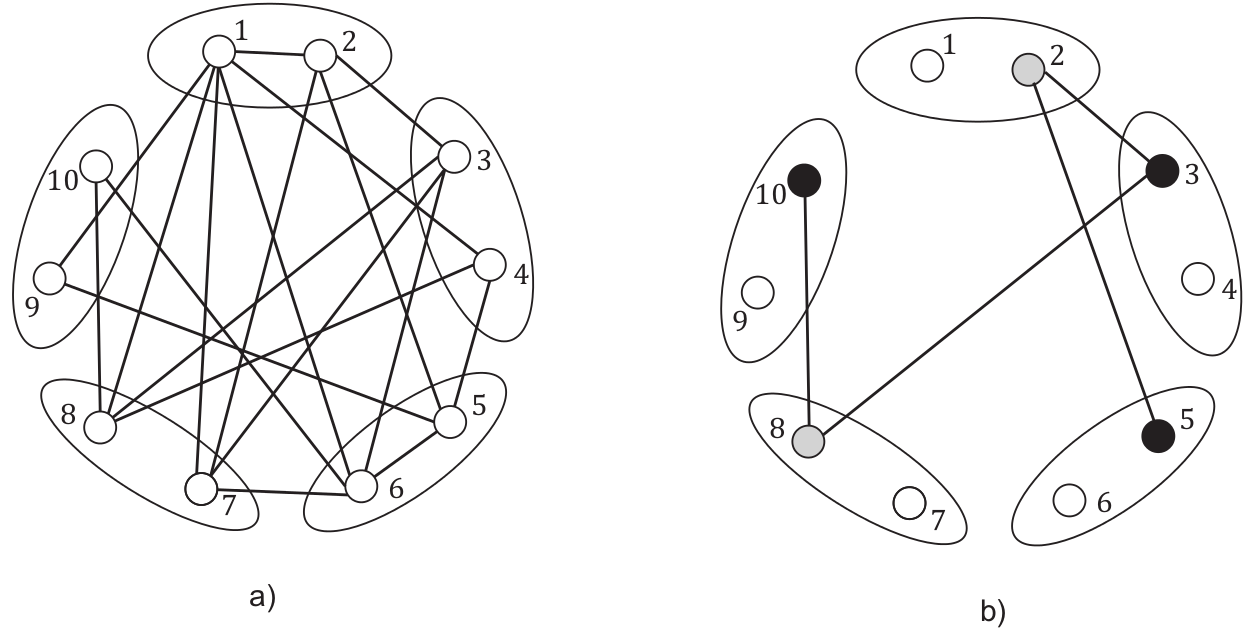
\includegraphics[scale=0.3]{figures/pcp.png}
\caption{(a) Shows a problem instance and (b) its solution.}
\label{pd:pcpExample}
\end{center}
\end{figure}


\section{Wavelength Routing and Assignment Problem}

The PCP has initially been considered by Li and Simha in \cite{li-00} and arises from considering the join problem of routing and wavelength assignment in WDM (Wavelength Division Multiplexing) optical networks. 

%The RWA problem takes two forms: static and dynamic
%[1]. In the static case, all connection requests are known in
%advance, thus a routing decision can be made based on the
%complete knowledge of the traffic to be served by the
%network. The static RWA problem is found to be NP-
%complete that cannot be solved exactly in a polynomial
%T
%This paper resulted from the research supported by the Serbian
%Ministry of science and technological development (project TR-11013).
%Goran Z. Marković is with the Faculty of Traffic and Transport
%Engineering, University of Belgrade, Serbia, Vojvode Stepe 305, 11000
%Belgrade, Serbia; (e-mail:g.markovic@sf.bg.ac.rs).
%Vladanka S. Aćimović-Raspopović is with the Faculty of Traffic and
%Transport Engineering, University of Belgrade, Serbia, Vojvode Stepe
%305, 11000 Beograd, Serbia; (e-mail:v.acimovic@sf.bg.ac.rs).
%time. In the dynamic case, a connection request has to be
%routed and wavelengths assigned independently of other
%connections, which either have already been assigned or
%will be assigned [1]-[3]

\section{Complexity}

%

% -- min-RWA --
%Erlebach and Jansen [7] showed that min-RWA
%is NP-hard. Several authors proposed different
%approximate algorithms for solving min-RWA.
%Banerjee and Mukherjee [4], Hyytia
% ̈ and Virtamo
%[10], and Li and Simha [12] decompose the prob-
%lem in two phases. In the first phase, one or more
%possible routes are computed for each lightpath,
%while in the second one route and one wavelength
%are assigned to each lightpath. The second phase is
%often solved as a colouring problem defined on a
%conflict graph. Manohar et al. [13] proposed the
%Greedy-EDP-RWA construction which was used
%in a multi-start procedure heuristic, in which both
%subproblems are solved simultaneously. Their
%algorithm is much faster and finds solutions as
%good as those found by the algorithm in [4].



%%%%%%%%%%%%%%%%%%%%%%%%%%%%%%%%%%%%%%%%%
\chapter{Previous Works}
\label{ch:previous}
%%%%%%%%%%%%%%%%%%%%%%%%%%%%%%%%%%%%%%%%%
This chapter provides an overview on previous works dealing with the Partition Coloring Problem. While the VCP has been studied extensively, only a few papers have been published on the PCP. So far, two exact approaches and three heuristics have been presented.

\section{Exact Approaches}

In 2010, Frota and Ribeiro presented a Branch-and-Cut algorithm for the PCP in \cite{frota-07}, which is based on a generalization of the 0-1 formulation for the VCP proposed in \cite{campelo-05,campelo-04}, called formulation of representatives. The branching strategy to decompose the problem into two subproblems is based on Mehrotra and Trick's branching rule \cite{trick-96}, that branches on two non-adjacent vertices. Improvements of linear relaxation bounds have been achieved by generalizing the original family of valid inequalites\cite{campelo-05,campelo-04}, based on \textit{External cuts} and \textit{Internal cuts}. For their experiments they used an AMD-Atlon machine with a 1.8 GHz clock and one Gbyte of RAM memory. Within 2 hours, each instance with up to 80 nodes and density of 0.5 could be solved to optimality. For instances with 90 nodes, only the ones with density $\geq 0.5$ could be solved to optimality in the same time. It is remarkable, that the algorithm performs worst on instances with a density between $0.3$ and $0.5$.\\
One year later, Hoshino et al. published a paper describing a Branch-and-Price algorithm, that performs ``far superior to the branch-and-cut algorithm in all instance classes tested''\cite{hoshino-11}. It uses a new formulation that combines the main ingredients of the formulation of representatives used in \cite{frota-07} and the classical independent set formulation presented in \cite{trick-96}. Campelo et al. previously proposed a combination of these formulations for the VCP in \cite{campelo-052}. For solving the pricing problem, which is equivalent to the classical maximum weighted independent set problem (MWIS), two different algorithms are used depending on the density of the graph. On a Pentium Core2 Quad 2.83 GHz with 8 Gb of RAM, an instance with 706 vertices and $101.600$ edges could have been solved, but the authors did not provide a hint on the time required.

\section{Heuristical Approaches}

Li and Simha introduced the PCP in \cite{li-00} as a subproblem of the min-RWA problem, proofed that it is as hard as VCP (which is $\mathcal{NP}$-complete \cite{karp-72}) and presented adaptions of the coloring heuristics \textit{Largest-First (LF)} by Welsh and Powell \cite{welsh-67}, \textit{Smallest-Last (SL)} by Matula et al. \cite{matula-72} and \textit{Color-Degree (CD)} by Brelaz \cite{brelaz-79} designed for VCP. Their results have shown, that \textit{CD} performed best, particularly the algorithm \textit{OneStepCD}. Therefore this heuristic is used in this work to create the initial solution and with a slight variation it is also used to improve it. It is worth to mention that in their paper, Li and Simha cite many papers dealing with theoretical aspects of graph coloring as well as min-RWA.\\

In their publication in 2006, Noronha et al. proposed a heuristic based on tabu search \cite{noronha-06}. Quite similar to the approach presented in this work, their strategy is to improve an existing solution by choosing a color $c$, assign an alternative coloring randomly to all clusters colored with $c$ and try to make the resulting solution feasible by using tabu search. In contrast, this work uses sophisticated algorithms to find alternative colorings. Their algorithm outperform the best previously known heuristic for partition coloring, and shows that it can improve the solution found by \textit{OneStepCD} by approximately 20\% in average. Beside PCP, the paper proposes advanced strategies for solving the min-RWA problem.

3. Hu, Raidl, Pop (2013): Memetic algorithm

We proposed a memetic algorithm (MA) for the partition graph coloring problem
that uses two distinct solution representations. For maintaining a diverse popula-
tion and to keep the computational effort for genetic operators low, we use a full
solution representation for crossover and mutation. In contrast, we use a more
compact and incomplete solution representation during local search. Both repre-
sentations work well in combination in the MA. During local search, we observed
that minimizing the number of colors results in many solutions of equal quality.
Therefore, we use a second evaluation criterion based on the number of conflicts
when using one color less. Computational experiments on common benchmark
instances sets show that although the MA is not always able to find the optimal
solutions, it produces solid results with very low run-times and therefore has
excellent scalability when it comes to large instances.
For future work, we want to consider a further incomplete solution represen-
tation which is based on characterizing the colors of the clusters. The challenge
will be to develop efficient algorithms for choosing the nodes in the clusters that
are compatible with the color assignments. We also want to consider further eval-
uation criteria besides color and conflicts so that more fine-tuned measurements
depending on specific situations are possible.

%%%%%%%%%%%%%%%%%%%%%%%%%%%%%%%%%%%%%%%%%
\chapter{Problem Solving Approach}
\label{ch:approach}
%%%%%%%%%%%%%%%%%%%%%%%%%%%%%%%%%%%%%%%%%
In this chapter, the algorithms and models of the hybrid approach for the PCP will be described and analyzed in detail. First in section \ref{sec:mainalg}, the main procedure is explained. Section \ref{sec:construction} then analyses the two different construction heuristics used in this work, namely \textit{OneStepCD} and \textit{DANGER}. The improvement phase is split into two parts: algorithms, that assign a new, but not mandatorily feasible coloring to a chosen set of nodes, here consisting of one random-, one heuristic- and two exact approaches, are applied in the first phase. In the following, this thesis will refer to these algorithms to as the ``recoloring'' algorithms \ref{sec:recoloring}. As for the second phase, section \ref{sec:tabu} presents the tabu search, which tries to find a coloring that makes the conflict-prone solution feasibly created by one of the recoloring algorithms. Additionally, two variants, one of them consisting in a modified ILP formulation and the other one in adding lately recolored areas to the tabu list, are considered in subsections of \ref{sec:recoloring} and \ref{sec:tabu}.

\section{Main Procedure}
\label{sec:mainalg}
The idea of the approach in general is to start from a feasible solution, pick a color and eliminate it. For each color $c$, the set of nodes colored with $c$ is exchanged with other nodes in the respecting clusters as well as recolored without considering color $c$. Using this strategy, it might not be possible to find a feasible solution. Therefore, infeasible solutions are accepted, i.e. solutions including at least one conflict, that is a pair of adjacent nodes $\{i,j\}\in E : i,j \in V$ colored with the same color. One of the two nodes is chosen and in the following referred to as the ``conflicting node''\footnote{How the node is chosen is shown in detail in \ref{sec:recoloring}}, its encasing cluster to as the ``conflicting cluster''. Further, a cluster is said to be of color $c$ if and only if it contains a selected node colored with color $c$. The conflicting clusters form the starting points for the tabu search, that tries to find an alternative color for each of them. This process eventually produces further conflicts, which then again have to be eliminated. If no feasible coloring can be found within a specified number of iterations, the next color $c+1$ is considered. If all conflicts can be eliminated, the algorithm has successfully decreased the chromatic number and repeats the whole process.\\
This approach differs from the strategy presented in \cite{noronha-06} mainly by the effort that is investigated in the recoloring phase. There, Noronha et.al. reassign colors in a random way and therefore produce a random number of conflicts. The main innovation presented in this work is the minimization of the number of conflicts produced by an advanced recoloring algorithm, with the intention to increase the chance of eliminating these conflicts by tabu search.\\
An example of a possible sequence of steps performed by the algorithm is given in Figure \ref{fig:mainproc}. There, a feasible solution is shown in figure \ref{fig:mainproc}a). The color dark grey is chosen to be eliminated. In the following two steps, for each darkgrey cluster, another node is chosen and colored with any color other than dark grey. After recoloring, the resulting graph shown in \ref{fig:mainproc}c) is infeasible. Then, starting from the conflicting cluster outlined in red, the tabu search looks up the node-color pair inside that cluster, that causes the fewest conflicts. In \ref{fig:mainproc}d), a node-color pair is found, which does not produce any new conflicts. If this solution would have produced conflicts again, the local search would go on searching until a feasible solution was found or the maximum amount of iteration was reached.
\ifx\du\undefined
  \newlength{\du}
\fi
\setlength{\du}{15\unitlength}
\begin{figure}
\begin{center}
\begin{tikzpicture}[scale=0.60]
\pgftransformxscale{1.000000}
\pgftransformyscale{-1.000000}
\definecolor{dialinecolor}{rgb}{0.000000, 0.000000, 0.000000}
\pgfsetstrokecolor{dialinecolor}
\definecolor{dialinecolor}{rgb}{1.000000, 1.000000, 1.000000}
\pgfsetfillcolor{dialinecolor}
\pgfsetlinewidth{0.050000\du}
\pgfsetdash{}{0pt}
\pgfsetdash{}{0pt}
\definecolor{dialinecolor}{rgb}{0.000000, 0.000000, 0.000000}
\pgfsetstrokecolor{dialinecolor}
\pgfpathellipse{\pgfpoint{13.300000\du}{3.150000\du}}{\pgfpoint{3.100000\du}{0\du}}{\pgfpoint{0\du}{1.800000\du}}
\pgfusepath{stroke}
\pgfsetlinewidth{0.050000\du}
\pgfsetdash{}{0pt}
\pgfsetdash{}{0pt}
\definecolor{dialinecolor}{rgb}{0.000000, 0.000000, 0.000000}
\pgfsetstrokecolor{dialinecolor}
\pgfpathellipse{\pgfpoint{4.200000\du}{3.100000\du}}{\pgfpoint{3.100000\du}{0\du}}{\pgfpoint{0\du}{1.800000\du}}
\pgfusepath{stroke}
\pgfsetlinewidth{0.050000\du}
\pgfsetdash{}{0pt}
\pgfsetdash{}{0pt}
\definecolor{dialinecolor}{rgb}{0.000000, 0.000000, 0.000000}
\pgfsetstrokecolor{dialinecolor}
\pgfpathellipse{\pgfpoint{13.350000\du}{13.125000\du}}{\pgfpoint{3.100000\du}{0\du}}{\pgfpoint{0\du}{1.800000\du}}
\pgfusepath{stroke}
\pgfsetlinewidth{0.050000\du}
\pgfsetdash{}{0pt}
\pgfsetdash{}{0pt}
\definecolor{dialinecolor}{rgb}{0.000000, 0.000000, 0.000000}
\pgfsetstrokecolor{dialinecolor}
\pgfpathellipse{\pgfpoint{4.165000\du}{13.075000\du}}{\pgfpoint{3.100000\du}{0\du}}{\pgfpoint{0\du}{1.800000\du}}
\pgfusepath{stroke}
\pgfsetlinewidth{0.050000\du}
\pgfsetdash{}{0pt}
\pgfsetdash{}{0pt}
\definecolor{dialinecolor}{rgb}{0.000000, 1.000000, 0.000000}
\pgfsetstrokecolor{dialinecolor}
\pgfpathellipse{\pgfpoint{4.145000\du}{8.075000\du}}{\pgfpoint{3.100000\du}{0\du}}{\pgfpoint{0\du}{1.800000\du}}
\pgfusepath{stroke}
\pgfsetlinewidth{0.050000\du}
\pgfsetdash{}{0pt}
\pgfsetdash{}{0pt}
\definecolor{dialinecolor}{rgb}{0.000000, 1.000000, 0.000000}
\pgfsetstrokecolor{dialinecolor}
\pgfpathellipse{\pgfpoint{13.230000\du}{8.175000\du}}{\pgfpoint{3.100000\du}{0\du}}{\pgfpoint{0\du}{1.800000\du}}
\pgfusepath{stroke}
\pgfsetlinewidth{0.050000\du}
\pgfsetdash{}{0pt}
\pgfsetdash{}{0pt}
\pgfsetbuttcap
\pgfsetmiterjoin
\pgfsetlinewidth{0.050000\du}
\pgfsetbuttcap
\pgfsetmiterjoin
\pgfsetdash{}{0pt}
\definecolor{dialinecolor}{rgb}{0.882353, 0.882353, 0.882353}
\pgfsetfillcolor{dialinecolor}
\pgfpathellipse{\pgfpoint{2.962500\du}{3.612500\du}}{\pgfpoint{0.462500\du}{0\du}}{\pgfpoint{0\du}{0.462500\du}}
\pgfusepath{fill}
\definecolor{dialinecolor}{rgb}{0.000000, 0.000000, 0.000000}
\pgfsetstrokecolor{dialinecolor}
\pgfpathellipse{\pgfpoint{2.962500\du}{3.612500\du}}{\pgfpoint{0.462500\du}{0\du}}{\pgfpoint{0\du}{0.462500\du}}
\pgfusepath{stroke}
\pgfsetbuttcap
\pgfsetmiterjoin
\pgfsetdash{}{0pt}
\definecolor{dialinecolor}{rgb}{0.000000, 0.000000, 0.000000}
\pgfsetstrokecolor{dialinecolor}
\pgfpathellipse{\pgfpoint{2.962500\du}{3.612500\du}}{\pgfpoint{0.462500\du}{0\du}}{\pgfpoint{0\du}{0.462500\du}}
\pgfusepath{stroke}
\pgfsetlinewidth{0.050000\du}
\pgfsetdash{{\pgflinewidth}{0.200000\du}}{0cm}
\pgfsetdash{{\pgflinewidth}{0.200000\du}}{0cm}
\pgfsetbuttcap
\pgfsetmiterjoin
\pgfsetlinewidth{0.050000\du}
\pgfsetbuttcap
\pgfsetmiterjoin
\pgfsetdash{{\pgflinewidth}{0.200000\du}}{0cm}
\definecolor{dialinecolor}{rgb}{1.000000, 1.000000, 1.000000}
\pgfsetfillcolor{dialinecolor}
\pgfpathellipse{\pgfpoint{4.947500\du}{2.562500\du}}{\pgfpoint{0.462500\du}{0\du}}{\pgfpoint{0\du}{0.462500\du}}
\pgfusepath{fill}
\definecolor{dialinecolor}{rgb}{0.000000, 0.000000, 0.000000}
\pgfsetstrokecolor{dialinecolor}
\pgfpathellipse{\pgfpoint{4.947500\du}{2.562500\du}}{\pgfpoint{0.462500\du}{0\du}}{\pgfpoint{0\du}{0.462500\du}}
\pgfusepath{stroke}
\pgfsetbuttcap
\pgfsetmiterjoin
\pgfsetdash{{\pgflinewidth}{0.200000\du}}{0cm}
\definecolor{dialinecolor}{rgb}{0.000000, 0.000000, 0.000000}
\pgfsetstrokecolor{dialinecolor}
\pgfpathellipse{\pgfpoint{4.947500\du}{2.562500\du}}{\pgfpoint{0.462500\du}{0\du}}{\pgfpoint{0\du}{0.462500\du}}
\pgfusepath{stroke}
\pgfsetlinewidth{0.050000\du}
\pgfsetdash{}{0pt}
\pgfsetdash{}{0pt}
\pgfsetbuttcap
\pgfsetmiterjoin
\pgfsetlinewidth{0.050000\du}
\pgfsetbuttcap
\pgfsetmiterjoin
\pgfsetdash{}{0pt}
\definecolor{dialinecolor}{rgb}{0.517647, 0.517647, 0.517647}
\pgfsetfillcolor{dialinecolor}
\pgfpathellipse{\pgfpoint{3.007500\du}{8.037500\du}}{\pgfpoint{0.462500\du}{0\du}}{\pgfpoint{0\du}{0.462500\du}}
\pgfusepath{fill}
\definecolor{dialinecolor}{rgb}{0.000000, 0.000000, 0.000000}
\pgfsetstrokecolor{dialinecolor}
\pgfpathellipse{\pgfpoint{3.007500\du}{8.037500\du}}{\pgfpoint{0.462500\du}{0\du}}{\pgfpoint{0\du}{0.462500\du}}
\pgfusepath{stroke}
\pgfsetbuttcap
\pgfsetmiterjoin
\pgfsetdash{}{0pt}
\definecolor{dialinecolor}{rgb}{0.000000, 0.000000, 0.000000}
\pgfsetstrokecolor{dialinecolor}
\pgfpathellipse{\pgfpoint{3.007500\du}{8.037500\du}}{\pgfpoint{0.462500\du}{0\du}}{\pgfpoint{0\du}{0.462500\du}}
\pgfusepath{stroke}
\pgfsetlinewidth{0.050000\du}
\pgfsetdash{{\pgflinewidth}{0.200000\du}}{0cm}
\pgfsetdash{{\pgflinewidth}{0.200000\du}}{0cm}
\pgfsetbuttcap
\pgfsetmiterjoin
\pgfsetlinewidth{0.050000\du}
\pgfsetbuttcap
\pgfsetmiterjoin
\pgfsetdash{{\pgflinewidth}{0.200000\du}}{0cm}
\definecolor{dialinecolor}{rgb}{1.000000, 1.000000, 1.000000}
\pgfsetfillcolor{dialinecolor}
\pgfpathellipse{\pgfpoint{5.092500\du}{8.037500\du}}{\pgfpoint{0.462500\du}{0\du}}{\pgfpoint{0\du}{0.462500\du}}
\pgfusepath{fill}
\definecolor{dialinecolor}{rgb}{0.000000, 0.000000, 0.000000}
\pgfsetstrokecolor{dialinecolor}
\pgfpathellipse{\pgfpoint{5.092500\du}{8.037500\du}}{\pgfpoint{0.462500\du}{0\du}}{\pgfpoint{0\du}{0.462500\du}}
\pgfusepath{stroke}
\pgfsetbuttcap
\pgfsetmiterjoin
\pgfsetdash{{\pgflinewidth}{0.200000\du}}{0cm}
\definecolor{dialinecolor}{rgb}{0.000000, 0.000000, 0.000000}
\pgfsetstrokecolor{dialinecolor}
\pgfpathellipse{\pgfpoint{5.092500\du}{8.037500\du}}{\pgfpoint{0.462500\du}{0\du}}{\pgfpoint{0\du}{0.462500\du}}
\pgfusepath{stroke}
\pgfsetlinewidth{0.050000\du}
\pgfsetdash{{\pgflinewidth}{0.200000\du}}{0cm}
\pgfsetdash{{\pgflinewidth}{0.200000\du}}{0cm}
\pgfsetbuttcap
\pgfsetmiterjoin
\pgfsetlinewidth{0.050000\du}
\pgfsetbuttcap
\pgfsetmiterjoin
\pgfsetdash{{\pgflinewidth}{0.200000\du}}{0cm}
\definecolor{dialinecolor}{rgb}{1.000000, 1.000000, 1.000000}
\pgfsetfillcolor{dialinecolor}
\pgfpathellipse{\pgfpoint{12.242500\du}{8.137500\du}}{\pgfpoint{0.462500\du}{0\du}}{\pgfpoint{0\du}{0.462500\du}}
\pgfusepath{fill}
\definecolor{dialinecolor}{rgb}{0.000000, 0.000000, 0.000000}
\pgfsetstrokecolor{dialinecolor}
\pgfpathellipse{\pgfpoint{12.242500\du}{8.137500\du}}{\pgfpoint{0.462500\du}{0\du}}{\pgfpoint{0\du}{0.462500\du}}
\pgfusepath{stroke}
\pgfsetbuttcap
\pgfsetmiterjoin
\pgfsetdash{{\pgflinewidth}{0.200000\du}}{0cm}
\definecolor{dialinecolor}{rgb}{0.000000, 0.000000, 0.000000}
\pgfsetstrokecolor{dialinecolor}
\pgfpathellipse{\pgfpoint{12.242500\du}{8.137500\du}}{\pgfpoint{0.462500\du}{0\du}}{\pgfpoint{0\du}{0.462500\du}}
\pgfusepath{stroke}
\pgfsetlinewidth{0.050000\du}
\pgfsetdash{}{0pt}
\pgfsetdash{}{0pt}
\pgfsetbuttcap
\pgfsetmiterjoin
\pgfsetlinewidth{0.050000\du}
\pgfsetbuttcap
\pgfsetmiterjoin
\pgfsetdash{}{0pt}
\definecolor{dialinecolor}{rgb}{0.517647, 0.517647, 0.517647}
\pgfsetfillcolor{dialinecolor}
\pgfpathellipse{\pgfpoint{14.327500\du}{8.137500\du}}{\pgfpoint{0.462500\du}{0\du}}{\pgfpoint{0\du}{0.462500\du}}
\pgfusepath{fill}
\definecolor{dialinecolor}{rgb}{0.000000, 0.000000, 0.000000}
\pgfsetstrokecolor{dialinecolor}
\pgfpathellipse{\pgfpoint{14.327500\du}{8.137500\du}}{\pgfpoint{0.462500\du}{0\du}}{\pgfpoint{0\du}{0.462500\du}}
\pgfusepath{stroke}
\pgfsetbuttcap
\pgfsetmiterjoin
\pgfsetdash{}{0pt}
\definecolor{dialinecolor}{rgb}{0.000000, 0.000000, 0.000000}
\pgfsetstrokecolor{dialinecolor}
\pgfpathellipse{\pgfpoint{14.327500\du}{8.137500\du}}{\pgfpoint{0.462500\du}{0\du}}{\pgfpoint{0\du}{0.462500\du}}
\pgfusepath{stroke}
\pgfsetlinewidth{0.050000\du}
\pgfsetdash{}{0pt}
\pgfsetdash{}{0pt}
\pgfsetbuttcap
\pgfsetmiterjoin
\pgfsetlinewidth{0.050000\du}
\pgfsetbuttcap
\pgfsetmiterjoin
\pgfsetdash{}{0pt}
\definecolor{dialinecolor}{rgb}{0.000000, 0.000000, 0.000000}
\pgfsetfillcolor{dialinecolor}
\pgfpathellipse{\pgfpoint{2.977500\du}{12.637500\du}}{\pgfpoint{0.462500\du}{0\du}}{\pgfpoint{0\du}{0.462500\du}}
\pgfusepath{fill}
\definecolor{dialinecolor}{rgb}{0.000000, 0.000000, 0.000000}
\pgfsetstrokecolor{dialinecolor}
\pgfpathellipse{\pgfpoint{2.977500\du}{12.637500\du}}{\pgfpoint{0.462500\du}{0\du}}{\pgfpoint{0\du}{0.462500\du}}
\pgfusepath{stroke}
\pgfsetbuttcap
\pgfsetmiterjoin
\pgfsetdash{}{0pt}
\definecolor{dialinecolor}{rgb}{0.000000, 0.000000, 0.000000}
\pgfsetstrokecolor{dialinecolor}
\pgfpathellipse{\pgfpoint{2.977500\du}{12.637500\du}}{\pgfpoint{0.462500\du}{0\du}}{\pgfpoint{0\du}{0.462500\du}}
\pgfusepath{stroke}
\pgfsetlinewidth{0.050000\du}
\pgfsetdash{{\pgflinewidth}{0.200000\du}}{0cm}
\pgfsetdash{{\pgflinewidth}{0.200000\du}}{0cm}
\pgfsetbuttcap
\pgfsetmiterjoin
\pgfsetlinewidth{0.050000\du}
\pgfsetbuttcap
\pgfsetmiterjoin
\pgfsetdash{{\pgflinewidth}{0.200000\du}}{0cm}
\definecolor{dialinecolor}{rgb}{1.000000, 1.000000, 1.000000}
\pgfsetfillcolor{dialinecolor}
\pgfpathellipse{\pgfpoint{5.012500\du}{13.587500\du}}{\pgfpoint{0.462500\du}{0\du}}{\pgfpoint{0\du}{0.462500\du}}
\pgfusepath{fill}
\definecolor{dialinecolor}{rgb}{0.000000, 0.000000, 0.000000}
\pgfsetstrokecolor{dialinecolor}
\pgfpathellipse{\pgfpoint{5.012500\du}{13.587500\du}}{\pgfpoint{0.462500\du}{0\du}}{\pgfpoint{0\du}{0.462500\du}}
\pgfusepath{stroke}
\pgfsetbuttcap
\pgfsetmiterjoin
\pgfsetdash{{\pgflinewidth}{0.200000\du}}{0cm}
\definecolor{dialinecolor}{rgb}{0.000000, 0.000000, 0.000000}
\pgfsetstrokecolor{dialinecolor}
\pgfpathellipse{\pgfpoint{5.012500\du}{13.587500\du}}{\pgfpoint{0.462500\du}{0\du}}{\pgfpoint{0\du}{0.462500\du}}
\pgfusepath{stroke}
\pgfsetlinewidth{0.050000\du}
\pgfsetdash{{\pgflinewidth}{0.200000\du}}{0cm}
\pgfsetdash{{\pgflinewidth}{0.200000\du}}{0cm}
\pgfsetbuttcap
\pgfsetmiterjoin
\pgfsetlinewidth{0.050000\du}
\pgfsetbuttcap
\pgfsetmiterjoin
\pgfsetdash{{\pgflinewidth}{0.200000\du}}{0cm}
\definecolor{dialinecolor}{rgb}{1.000000, 1.000000, 1.000000}
\pgfsetfillcolor{dialinecolor}
\pgfpathellipse{\pgfpoint{12.372500\du}{2.587500\du}}{\pgfpoint{0.462500\du}{0\du}}{\pgfpoint{0\du}{0.462500\du}}
\pgfusepath{fill}
\definecolor{dialinecolor}{rgb}{0.000000, 0.000000, 0.000000}
\pgfsetstrokecolor{dialinecolor}
\pgfpathellipse{\pgfpoint{12.372500\du}{2.587500\du}}{\pgfpoint{0.462500\du}{0\du}}{\pgfpoint{0\du}{0.462500\du}}
\pgfusepath{stroke}
\pgfsetbuttcap
\pgfsetmiterjoin
\pgfsetdash{{\pgflinewidth}{0.200000\du}}{0cm}
\definecolor{dialinecolor}{rgb}{0.000000, 0.000000, 0.000000}
\pgfsetstrokecolor{dialinecolor}
\pgfpathellipse{\pgfpoint{12.372500\du}{2.587500\du}}{\pgfpoint{0.462500\du}{0\du}}{\pgfpoint{0\du}{0.462500\du}}
\pgfusepath{stroke}
\pgfsetlinewidth{0.050000\du}
\pgfsetdash{}{0pt}
\pgfsetdash{}{0pt}
\pgfsetbuttcap
\pgfsetmiterjoin
\pgfsetlinewidth{0.050000\du}
\pgfsetbuttcap
\pgfsetmiterjoin
\pgfsetdash{}{0pt}
\definecolor{dialinecolor}{rgb}{0.882353, 0.882353, 0.882353}
\pgfsetfillcolor{dialinecolor}
\pgfpathellipse{\pgfpoint{14.307500\du}{3.837500\du}}{\pgfpoint{0.462500\du}{0\du}}{\pgfpoint{0\du}{0.462500\du}}
\pgfusepath{fill}
\definecolor{dialinecolor}{rgb}{0.000000, 0.000000, 0.000000}
\pgfsetstrokecolor{dialinecolor}
\pgfpathellipse{\pgfpoint{14.307500\du}{3.837500\du}}{\pgfpoint{0.462500\du}{0\du}}{\pgfpoint{0\du}{0.462500\du}}
\pgfusepath{stroke}
\pgfsetbuttcap
\pgfsetmiterjoin
\pgfsetdash{}{0pt}
\definecolor{dialinecolor}{rgb}{0.000000, 0.000000, 0.000000}
\pgfsetstrokecolor{dialinecolor}
\pgfpathellipse{\pgfpoint{14.307500\du}{3.837500\du}}{\pgfpoint{0.462500\du}{0\du}}{\pgfpoint{0\du}{0.462500\du}}
\pgfusepath{stroke}
\pgfsetlinewidth{0.050000\du}
\pgfsetdash{{\pgflinewidth}{0.200000\du}}{0cm}
\pgfsetdash{{\pgflinewidth}{0.200000\du}}{0cm}
\pgfsetbuttcap
\pgfsetmiterjoin
\pgfsetlinewidth{0.050000\du}
\pgfsetbuttcap
\pgfsetmiterjoin
\pgfsetdash{{\pgflinewidth}{0.200000\du}}{0cm}
\definecolor{dialinecolor}{rgb}{1.000000, 1.000000, 1.000000}
\pgfsetfillcolor{dialinecolor}
\pgfpathellipse{\pgfpoint{12.312500\du}{13.587500\du}}{\pgfpoint{0.462500\du}{0\du}}{\pgfpoint{0\du}{0.462500\du}}
\pgfusepath{fill}
\definecolor{dialinecolor}{rgb}{0.000000, 0.000000, 0.000000}
\pgfsetstrokecolor{dialinecolor}
\pgfpathellipse{\pgfpoint{12.312500\du}{13.587500\du}}{\pgfpoint{0.462500\du}{0\du}}{\pgfpoint{0\du}{0.462500\du}}
\pgfusepath{stroke}
\pgfsetbuttcap
\pgfsetmiterjoin
\pgfsetdash{{\pgflinewidth}{0.200000\du}}{0cm}
\definecolor{dialinecolor}{rgb}{0.000000, 0.000000, 0.000000}
\pgfsetstrokecolor{dialinecolor}
\pgfpathellipse{\pgfpoint{12.312500\du}{13.587500\du}}{\pgfpoint{0.462500\du}{0\du}}{\pgfpoint{0\du}{0.462500\du}}
\pgfusepath{stroke}
\pgfsetlinewidth{0.050000\du}
\pgfsetdash{}{0pt}
\pgfsetdash{}{0pt}
\pgfsetbuttcap
\pgfsetmiterjoin
\pgfsetlinewidth{0.050000\du}
\pgfsetbuttcap
\pgfsetmiterjoin
\pgfsetdash{}{0pt}
\definecolor{dialinecolor}{rgb}{0.000000, 0.000000, 0.000000}
\pgfsetfillcolor{dialinecolor}
\pgfpathellipse{\pgfpoint{14.247500\du}{12.687500\du}}{\pgfpoint{0.462500\du}{0\du}}{\pgfpoint{0\du}{0.462500\du}}
\pgfusepath{fill}
\definecolor{dialinecolor}{rgb}{0.000000, 0.000000, 0.000000}
\pgfsetstrokecolor{dialinecolor}
\pgfpathellipse{\pgfpoint{14.247500\du}{12.687500\du}}{\pgfpoint{0.462500\du}{0\du}}{\pgfpoint{0\du}{0.462500\du}}
\pgfusepath{stroke}
\pgfsetbuttcap
\pgfsetmiterjoin
\pgfsetdash{}{0pt}
\definecolor{dialinecolor}{rgb}{0.000000, 0.000000, 0.000000}
\pgfsetstrokecolor{dialinecolor}
\pgfpathellipse{\pgfpoint{14.247500\du}{12.687500\du}}{\pgfpoint{0.462500\du}{0\du}}{\pgfpoint{0\du}{0.462500\du}}
\pgfusepath{stroke}
\pgfsetlinewidth{0.050000\du}
\pgfsetdash{}{0pt}
\pgfsetdash{}{0pt}
\pgfsetbuttcap
{
\definecolor{dialinecolor}{rgb}{0.000000, 0.000000, 0.000000}
\pgfsetfillcolor{dialinecolor}
% was here!!!
\definecolor{dialinecolor}{rgb}{0.000000, 0.000000, 0.000000}
\pgfsetstrokecolor{dialinecolor}
\draw (2.967713\du,4.125113\du)--(3.002287\du,7.524887\du);
}
\pgfsetlinewidth{0.050000\du}
\pgfsetdash{}{0pt}
\pgfsetdash{}{0pt}
\pgfsetbuttcap
{
\definecolor{dialinecolor}{rgb}{0.000000, 0.000000, 0.000000}
\pgfsetfillcolor{dialinecolor}
% was here!!!
\definecolor{dialinecolor}{rgb}{0.000000, 0.000000, 0.000000}
\pgfsetstrokecolor{dialinecolor}
\draw (3.004156\du,8.550171\du)--(2.980844\du,12.124829\du);
}
\pgfsetlinewidth{0.050000\du}
\pgfsetdash{{\pgflinewidth}{0.200000\du}}{0cm}
\pgfsetdash{{\pgflinewidth}{0.200000\du}}{0cm}
\pgfsetbuttcap
{
\definecolor{dialinecolor}{rgb}{0.000000, 0.000000, 0.000000}
\pgfsetfillcolor{dialinecolor}
% was here!!!
\definecolor{dialinecolor}{rgb}{0.000000, 0.000000, 0.000000}
\pgfsetstrokecolor{dialinecolor}
\draw (3.184028\du,4.072717\du)--(4.870972\du,7.577283\du);
}
\pgfsetlinewidth{0.050000\du}
\pgfsetdash{{\pgflinewidth}{0.200000\du}}{0cm}
\pgfsetdash{{\pgflinewidth}{0.200000\du}}{0cm}
\pgfsetbuttcap
{
\definecolor{dialinecolor}{rgb}{0.000000, 0.000000, 0.000000}
\pgfsetfillcolor{dialinecolor}
% was here!!!
\definecolor{dialinecolor}{rgb}{0.000000, 0.000000, 0.000000}
\pgfsetstrokecolor{dialinecolor}
\draw (5.459600\du,2.564224\du)--(11.860400\du,2.585776\du);
}
\pgfsetlinewidth{0.050000\du}
\pgfsetdash{{\pgflinewidth}{0.200000\du}}{0cm}
\pgfsetdash{{\pgflinewidth}{0.200000\du}}{0cm}
\pgfsetbuttcap
{
\definecolor{dialinecolor}{rgb}{0.000000, 0.000000, 0.000000}
\pgfsetfillcolor{dialinecolor}
% was here!!!
\definecolor{dialinecolor}{rgb}{0.000000, 0.000000, 0.000000}
\pgfsetstrokecolor{dialinecolor}
\draw (3.434417\du,12.415576\du)--(11.785583\du,8.359424\du);
}
\pgfsetlinewidth{0.050000\du}
\pgfsetdash{{\pgflinewidth}{0.200000\du}}{0cm}
\pgfsetdash{{\pgflinewidth}{0.200000\du}}{0cm}
\pgfsetbuttcap
{
\definecolor{dialinecolor}{rgb}{0.000000, 0.000000, 0.000000}
\pgfsetfillcolor{dialinecolor}
% was here!!!
\definecolor{dialinecolor}{rgb}{0.000000, 0.000000, 0.000000}
\pgfsetstrokecolor{dialinecolor}
\draw (5.502178\du,7.730804\du)--(11.962822\du,2.894196\du);
}
\pgfsetlinewidth{0.050000\du}
\pgfsetdash{{\pgflinewidth}{0.200000\du}}{0cm}
\pgfsetdash{{\pgflinewidth}{0.200000\du}}{0cm}
\pgfsetbuttcap
{
\definecolor{dialinecolor}{rgb}{0.000000, 0.000000, 0.000000}
\pgfsetfillcolor{dialinecolor}
% was here!!!
\definecolor{dialinecolor}{rgb}{0.000000, 0.000000, 0.000000}
\pgfsetstrokecolor{dialinecolor}
\draw (5.297529\du,13.161505\du)--(12.087471\du,3.013495\du);
}
\pgfsetlinewidth{0.050000\du}
\pgfsetdash{}{0pt}
\pgfsetdash{}{0pt}
\pgfsetbuttcap
{
\definecolor{dialinecolor}{rgb}{0.000000, 0.000000, 0.000000}
\pgfsetfillcolor{dialinecolor}
% was here!!!
\definecolor{dialinecolor}{rgb}{0.000000, 0.000000, 0.000000}
\pgfsetstrokecolor{dialinecolor}
\draw (14.309885\du,4.350330\du)--(14.325115\du,7.624670\du);
}
\pgfsetlinewidth{0.050000\du}
\pgfsetdash{}{0pt}
\pgfsetdash{}{0pt}
\pgfsetbuttcap
{
\definecolor{dialinecolor}{rgb}{0.000000, 0.000000, 0.000000}
\pgfsetfillcolor{dialinecolor}
% was here!!!
\definecolor{dialinecolor}{rgb}{0.000000, 0.000000, 0.000000}
\pgfsetstrokecolor{dialinecolor}
\draw (14.256504\du,12.175403\du)--(14.318496\du,8.649597\du);
}
\pgfsetlinewidth{0.050000\du}
\pgfsetdash{{\pgflinewidth}{0.200000\du}}{0cm}
\pgfsetdash{{\pgflinewidth}{0.200000\du}}{0cm}
\pgfsetbuttcap
{
\definecolor{dialinecolor}{rgb}{0.000000, 0.000000, 0.000000}
\pgfsetfillcolor{dialinecolor}
% was here!!!
\definecolor{dialinecolor}{rgb}{0.000000, 0.000000, 0.000000}
\pgfsetstrokecolor{dialinecolor}
\draw (14.040685\du,12.218170\du)--(12.449315\du,8.606830\du);
}
\pgfsetlinewidth{0.050000\du}
\pgfsetdash{{\pgflinewidth}{0.200000\du}}{0cm}
\pgfsetdash{{\pgflinewidth}{0.200000\du}}{0cm}
\pgfsetbuttcap
{
\definecolor{dialinecolor}{rgb}{0.000000, 0.000000, 0.000000}
\pgfsetfillcolor{dialinecolor}
% was here!!!
\definecolor{dialinecolor}{rgb}{0.000000, 0.000000, 0.000000}
\pgfsetstrokecolor{dialinecolor}
\draw (14.085548\du,4.299677\du)--(12.464452\du,7.675323\du);
}
\pgfsetlinewidth{0.050000\du}
\pgfsetdash{{\pgflinewidth}{0.200000\du}}{0cm}
\pgfsetdash{{\pgflinewidth}{0.200000\du}}{0cm}
\pgfsetbuttcap
{
\definecolor{dialinecolor}{rgb}{0.000000, 0.000000, 0.000000}
\pgfsetfillcolor{dialinecolor}
% was here!!!
\definecolor{dialinecolor}{rgb}{0.000000, 0.000000, 0.000000}
\pgfsetstrokecolor{dialinecolor}
\draw (12.249084\du,8.650101\du)--(12.305916\du,13.074899\du);
}
\pgfsetlinewidth{0.050000\du}
\pgfsetdash{{\pgflinewidth}{0.200000\du}}{0cm}
\pgfsetdash{{\pgflinewidth}{0.200000\du}}{0cm}
\pgfsetbuttcap
{
\definecolor{dialinecolor}{rgb}{0.000000, 0.000000, 0.000000}
\pgfsetfillcolor{dialinecolor}
% was here!!!
\definecolor{dialinecolor}{rgb}{0.000000, 0.000000, 0.000000}
\pgfsetstrokecolor{dialinecolor}
\draw (5.354460\du,2.873508\du)--(11.835540\du,7.826492\du);
}
\pgfsetlinewidth{0.050000\du}
\pgfsetdash{}{0pt}
\pgfsetdash{}{0pt}
\pgfsetbuttcap
{
\definecolor{dialinecolor}{rgb}{0.000000, 0.000000, 0.000000}
\pgfsetfillcolor{dialinecolor}
% was here!!!
\definecolor{dialinecolor}{rgb}{0.000000, 0.000000, 0.000000}
\pgfsetstrokecolor{dialinecolor}
\pgfpathmoveto{\pgfpoint{14.729769\du}{12.514532\du}}
\pgfpatharc{68}{-66}{4.625925\du and 4.625925\du}
\pgfusepath{stroke}
}
\pgfsetlinewidth{0.050000\du}
\pgfsetdash{}{0pt}
\pgfsetdash{}{0pt}
\pgfsetbuttcap
{
\definecolor{dialinecolor}{rgb}{0.000000, 0.000000, 0.000000}
\pgfsetfillcolor{dialinecolor}
% was here!!!
\definecolor{dialinecolor}{rgb}{0.000000, 0.000000, 0.000000}
\pgfsetstrokecolor{dialinecolor}
\pgfpathmoveto{\pgfpoint{2.487719\du}{3.805784\du}}
\pgfpatharc{245}{116}{4.771862\du and 4.771862\du}
\pgfusepath{stroke}
}
\pgfsetlinewidth{0.050000\du}
\pgfsetdash{}{0pt}
\pgfsetdash{}{0pt}
\definecolor{dialinecolor}{rgb}{0.000000, 0.000000, 0.000000}
\pgfsetstrokecolor{dialinecolor}
\pgfpathellipse{\pgfpoint{34.620200\du}{3.225000\du}}{\pgfpoint{3.100000\du}{0\du}}{\pgfpoint{0\du}{1.800000\du}}
\pgfusepath{stroke}
\pgfsetlinewidth{0.050000\du}
\pgfsetdash{}{0pt}
\pgfsetdash{}{0pt}
\definecolor{dialinecolor}{rgb}{0.000000, 0.000000, 0.000000}
\pgfsetstrokecolor{dialinecolor}
\pgfpathellipse{\pgfpoint{25.520200\du}{3.175000\du}}{\pgfpoint{3.100000\du}{0\du}}{\pgfpoint{0\du}{1.800000\du}}
\pgfusepath{stroke}
\pgfsetlinewidth{0.050000\du}
\pgfsetdash{}{0pt}
\pgfsetdash{}{0pt}
\definecolor{dialinecolor}{rgb}{0.000000, 0.000000, 0.000000}
\pgfsetstrokecolor{dialinecolor}
\pgfpathellipse{\pgfpoint{34.670200\du}{13.200000\du}}{\pgfpoint{3.100000\du}{0\du}}{\pgfpoint{0\du}{1.800000\du}}
\pgfusepath{stroke}
\pgfsetlinewidth{0.050000\du}
\pgfsetdash{}{0pt}
\pgfsetdash{}{0pt}
\definecolor{dialinecolor}{rgb}{0.000000, 0.000000, 0.000000}
\pgfsetstrokecolor{dialinecolor}
\pgfpathellipse{\pgfpoint{25.485200\du}{13.150000\du}}{\pgfpoint{3.100000\du}{0\du}}{\pgfpoint{0\du}{1.800000\du}}
\pgfusepath{stroke}
\pgfsetlinewidth{0.050000\du}
\pgfsetdash{}{0pt}
\pgfsetdash{}{0pt}
\definecolor{dialinecolor}{rgb}{0.000000, 0.000000, 0.000000}
\pgfsetstrokecolor{dialinecolor}
\pgfpathellipse{\pgfpoint{25.465200\du}{8.150000\du}}{\pgfpoint{3.100000\du}{0\du}}{\pgfpoint{0\du}{1.800000\du}}
\pgfusepath{stroke}
\pgfsetlinewidth{0.050000\du}
\pgfsetdash{}{0pt}
\pgfsetdash{}{0pt}
\definecolor{dialinecolor}{rgb}{0.000000, 1.000000, 0.000000}
\pgfsetstrokecolor{dialinecolor}
\pgfpathellipse{\pgfpoint{34.550200\du}{8.250000\du}}{\pgfpoint{3.100000\du}{0\du}}{\pgfpoint{0\du}{1.800000\du}}
\pgfusepath{stroke}
\pgfsetlinewidth{0.050000\du}
\pgfsetdash{}{0pt}
\pgfsetdash{}{0pt}
\pgfsetbuttcap
\pgfsetmiterjoin
\pgfsetlinewidth{0.050000\du}
\pgfsetbuttcap
\pgfsetmiterjoin
\pgfsetdash{}{0pt}
\definecolor{dialinecolor}{rgb}{0.882353, 0.882353, 0.882353}
\pgfsetfillcolor{dialinecolor}
\pgfpathellipse{\pgfpoint{24.282700\du}{3.687500\du}}{\pgfpoint{0.462500\du}{0\du}}{\pgfpoint{0\du}{0.462500\du}}
\pgfusepath{fill}
\definecolor{dialinecolor}{rgb}{0.000000, 0.000000, 0.000000}
\pgfsetstrokecolor{dialinecolor}
\pgfpathellipse{\pgfpoint{24.282700\du}{3.687500\du}}{\pgfpoint{0.462500\du}{0\du}}{\pgfpoint{0\du}{0.462500\du}}
\pgfusepath{stroke}
\pgfsetbuttcap
\pgfsetmiterjoin
\pgfsetdash{}{0pt}
\definecolor{dialinecolor}{rgb}{0.000000, 0.000000, 0.000000}
\pgfsetstrokecolor{dialinecolor}
\pgfpathellipse{\pgfpoint{24.282700\du}{3.687500\du}}{\pgfpoint{0.462500\du}{0\du}}{\pgfpoint{0\du}{0.462500\du}}
\pgfusepath{stroke}
\pgfsetlinewidth{0.050000\du}
\pgfsetdash{{\pgflinewidth}{0.200000\du}}{0cm}
\pgfsetdash{{\pgflinewidth}{0.200000\du}}{0cm}
\pgfsetbuttcap
\pgfsetmiterjoin
\pgfsetlinewidth{0.050000\du}
\pgfsetbuttcap
\pgfsetmiterjoin
\pgfsetdash{{\pgflinewidth}{0.200000\du}}{0cm}
\definecolor{dialinecolor}{rgb}{1.000000, 1.000000, 1.000000}
\pgfsetfillcolor{dialinecolor}
\pgfpathellipse{\pgfpoint{26.267700\du}{2.637500\du}}{\pgfpoint{0.462500\du}{0\du}}{\pgfpoint{0\du}{0.462500\du}}
\pgfusepath{fill}
\definecolor{dialinecolor}{rgb}{0.000000, 0.000000, 0.000000}
\pgfsetstrokecolor{dialinecolor}
\pgfpathellipse{\pgfpoint{26.267700\du}{2.637500\du}}{\pgfpoint{0.462500\du}{0\du}}{\pgfpoint{0\du}{0.462500\du}}
\pgfusepath{stroke}
\pgfsetbuttcap
\pgfsetmiterjoin
\pgfsetdash{{\pgflinewidth}{0.200000\du}}{0cm}
\definecolor{dialinecolor}{rgb}{0.000000, 0.000000, 0.000000}
\pgfsetstrokecolor{dialinecolor}
\pgfpathellipse{\pgfpoint{26.267700\du}{2.637500\du}}{\pgfpoint{0.462500\du}{0\du}}{\pgfpoint{0\du}{0.462500\du}}
\pgfusepath{stroke}
\pgfsetlinewidth{0.050000\du}
\pgfsetdash{{\pgflinewidth}{0.200000\du}}{0cm}
\pgfsetdash{{\pgflinewidth}{0.200000\du}}{0cm}
\pgfsetbuttcap
\pgfsetmiterjoin
\pgfsetlinewidth{0.050000\du}
\pgfsetbuttcap
\pgfsetmiterjoin
\pgfsetdash{{\pgflinewidth}{0.200000\du}}{0cm}
\definecolor{dialinecolor}{rgb}{1.000000, 1.000000, 1.000000}
\pgfsetfillcolor{dialinecolor}
\pgfpathellipse{\pgfpoint{24.327700\du}{8.112500\du}}{\pgfpoint{0.462500\du}{0\du}}{\pgfpoint{0\du}{0.462500\du}}
\pgfusepath{fill}
\definecolor{dialinecolor}{rgb}{0.000000, 0.000000, 0.000000}
\pgfsetstrokecolor{dialinecolor}
\pgfpathellipse{\pgfpoint{24.327700\du}{8.112500\du}}{\pgfpoint{0.462500\du}{0\du}}{\pgfpoint{0\du}{0.462500\du}}
\pgfusepath{stroke}
\pgfsetbuttcap
\pgfsetmiterjoin
\pgfsetdash{{\pgflinewidth}{0.200000\du}}{0cm}
\definecolor{dialinecolor}{rgb}{0.000000, 0.000000, 0.000000}
\pgfsetstrokecolor{dialinecolor}
\pgfpathellipse{\pgfpoint{24.327700\du}{8.112500\du}}{\pgfpoint{0.462500\du}{0\du}}{\pgfpoint{0\du}{0.462500\du}}
\pgfusepath{stroke}
\pgfsetlinewidth{0.050000\du}
\pgfsetdash{}{0pt}
\pgfsetdash{}{0pt}
\pgfsetbuttcap
\pgfsetmiterjoin
\pgfsetlinewidth{0.050000\du}
\pgfsetbuttcap
\pgfsetmiterjoin
\pgfsetdash{}{0pt}
\definecolor{dialinecolor}{rgb}{0.000000, 0.000000, 0.000000}
\pgfsetfillcolor{dialinecolor}
\pgfpathellipse{\pgfpoint{26.412700\du}{8.112500\du}}{\pgfpoint{0.462500\du}{0\du}}{\pgfpoint{0\du}{0.462500\du}}
\pgfusepath{fill}
\definecolor{dialinecolor}{rgb}{0.000000, 0.000000, 0.000000}
\pgfsetstrokecolor{dialinecolor}
\pgfpathellipse{\pgfpoint{26.412700\du}{8.112500\du}}{\pgfpoint{0.462500\du}{0\du}}{\pgfpoint{0\du}{0.462500\du}}
\pgfusepath{stroke}
\pgfsetbuttcap
\pgfsetmiterjoin
\pgfsetdash{}{0pt}
\definecolor{dialinecolor}{rgb}{0.000000, 0.000000, 0.000000}
\pgfsetstrokecolor{dialinecolor}
\pgfpathellipse{\pgfpoint{26.412700\du}{8.112500\du}}{\pgfpoint{0.462500\du}{0\du}}{\pgfpoint{0\du}{0.462500\du}}
\pgfusepath{stroke}
\pgfsetlinewidth{0.050000\du}
\pgfsetdash{{\pgflinewidth}{0.200000\du}}{0cm}
\pgfsetdash{{\pgflinewidth}{0.200000\du}}{0cm}
\pgfsetbuttcap
\pgfsetmiterjoin
\pgfsetlinewidth{0.050000\du}
\pgfsetbuttcap
\pgfsetmiterjoin
\pgfsetdash{{\pgflinewidth}{0.200000\du}}{0cm}
\definecolor{dialinecolor}{rgb}{1.000000, 1.000000, 1.000000}
\pgfsetfillcolor{dialinecolor}
\pgfpathellipse{\pgfpoint{33.562700\du}{8.212500\du}}{\pgfpoint{0.462500\du}{0\du}}{\pgfpoint{0\du}{0.462500\du}}
\pgfusepath{fill}
\definecolor{dialinecolor}{rgb}{0.000000, 0.000000, 0.000000}
\pgfsetstrokecolor{dialinecolor}
\pgfpathellipse{\pgfpoint{33.562700\du}{8.212500\du}}{\pgfpoint{0.462500\du}{0\du}}{\pgfpoint{0\du}{0.462500\du}}
\pgfusepath{stroke}
\pgfsetbuttcap
\pgfsetmiterjoin
\pgfsetdash{{\pgflinewidth}{0.200000\du}}{0cm}
\definecolor{dialinecolor}{rgb}{0.000000, 0.000000, 0.000000}
\pgfsetstrokecolor{dialinecolor}
\pgfpathellipse{\pgfpoint{33.562700\du}{8.212500\du}}{\pgfpoint{0.462500\du}{0\du}}{\pgfpoint{0\du}{0.462500\du}}
\pgfusepath{stroke}
\pgfsetlinewidth{0.050000\du}
\pgfsetdash{}{0pt}
\pgfsetdash{}{0pt}
\pgfsetbuttcap
\pgfsetmiterjoin
\pgfsetlinewidth{0.050000\du}
\pgfsetbuttcap
\pgfsetmiterjoin
\pgfsetdash{}{0pt}
\definecolor{dialinecolor}{rgb}{0.517647, 0.517647, 0.517647}
\pgfsetfillcolor{dialinecolor}
\pgfpathellipse{\pgfpoint{35.647700\du}{8.212500\du}}{\pgfpoint{0.462500\du}{0\du}}{\pgfpoint{0\du}{0.462500\du}}
\pgfusepath{fill}
\definecolor{dialinecolor}{rgb}{0.000000, 0.000000, 0.000000}
\pgfsetstrokecolor{dialinecolor}
\pgfpathellipse{\pgfpoint{35.647700\du}{8.212500\du}}{\pgfpoint{0.462500\du}{0\du}}{\pgfpoint{0\du}{0.462500\du}}
\pgfusepath{stroke}
\pgfsetbuttcap
\pgfsetmiterjoin
\pgfsetdash{}{0pt}
\definecolor{dialinecolor}{rgb}{0.000000, 0.000000, 0.000000}
\pgfsetstrokecolor{dialinecolor}
\pgfpathellipse{\pgfpoint{35.647700\du}{8.212500\du}}{\pgfpoint{0.462500\du}{0\du}}{\pgfpoint{0\du}{0.462500\du}}
\pgfusepath{stroke}
\pgfsetlinewidth{0.050000\du}
\pgfsetdash{}{0pt}
\pgfsetdash{}{0pt}
\pgfsetbuttcap
\pgfsetmiterjoin
\pgfsetlinewidth{0.050000\du}
\pgfsetbuttcap
\pgfsetmiterjoin
\pgfsetdash{}{0pt}
\definecolor{dialinecolor}{rgb}{0.000000, 0.000000, 0.000000}
\pgfsetfillcolor{dialinecolor}
\pgfpathellipse{\pgfpoint{24.297700\du}{12.712500\du}}{\pgfpoint{0.462500\du}{0\du}}{\pgfpoint{0\du}{0.462500\du}}
\pgfusepath{fill}
\definecolor{dialinecolor}{rgb}{0.000000, 0.000000, 0.000000}
\pgfsetstrokecolor{dialinecolor}
\pgfpathellipse{\pgfpoint{24.297700\du}{12.712500\du}}{\pgfpoint{0.462500\du}{0\du}}{\pgfpoint{0\du}{0.462500\du}}
\pgfusepath{stroke}
\pgfsetbuttcap
\pgfsetmiterjoin
\pgfsetdash{}{0pt}
\definecolor{dialinecolor}{rgb}{0.000000, 0.000000, 0.000000}
\pgfsetstrokecolor{dialinecolor}
\pgfpathellipse{\pgfpoint{24.297700\du}{12.712500\du}}{\pgfpoint{0.462500\du}{0\du}}{\pgfpoint{0\du}{0.462500\du}}
\pgfusepath{stroke}
\pgfsetlinewidth{0.050000\du}
\pgfsetdash{{\pgflinewidth}{0.200000\du}}{0cm}
\pgfsetdash{{\pgflinewidth}{0.200000\du}}{0cm}
\pgfsetbuttcap
\pgfsetmiterjoin
\pgfsetlinewidth{0.050000\du}
\pgfsetbuttcap
\pgfsetmiterjoin
\pgfsetdash{{\pgflinewidth}{0.200000\du}}{0cm}
\definecolor{dialinecolor}{rgb}{1.000000, 1.000000, 1.000000}
\pgfsetfillcolor{dialinecolor}
\pgfpathellipse{\pgfpoint{26.332700\du}{13.662500\du}}{\pgfpoint{0.462500\du}{0\du}}{\pgfpoint{0\du}{0.462500\du}}
\pgfusepath{fill}
\definecolor{dialinecolor}{rgb}{0.000000, 0.000000, 0.000000}
\pgfsetstrokecolor{dialinecolor}
\pgfpathellipse{\pgfpoint{26.332700\du}{13.662500\du}}{\pgfpoint{0.462500\du}{0\du}}{\pgfpoint{0\du}{0.462500\du}}
\pgfusepath{stroke}
\pgfsetbuttcap
\pgfsetmiterjoin
\pgfsetdash{{\pgflinewidth}{0.200000\du}}{0cm}
\definecolor{dialinecolor}{rgb}{0.000000, 0.000000, 0.000000}
\pgfsetstrokecolor{dialinecolor}
\pgfpathellipse{\pgfpoint{26.332700\du}{13.662500\du}}{\pgfpoint{0.462500\du}{0\du}}{\pgfpoint{0\du}{0.462500\du}}
\pgfusepath{stroke}
\pgfsetlinewidth{0.050000\du}
\pgfsetdash{{\pgflinewidth}{0.200000\du}}{0cm}
\pgfsetdash{{\pgflinewidth}{0.200000\du}}{0cm}
\pgfsetbuttcap
\pgfsetmiterjoin
\pgfsetlinewidth{0.050000\du}
\pgfsetbuttcap
\pgfsetmiterjoin
\pgfsetdash{{\pgflinewidth}{0.200000\du}}{0cm}
\definecolor{dialinecolor}{rgb}{1.000000, 1.000000, 1.000000}
\pgfsetfillcolor{dialinecolor}
\pgfpathellipse{\pgfpoint{33.692700\du}{2.662500\du}}{\pgfpoint{0.462500\du}{0\du}}{\pgfpoint{0\du}{0.462500\du}}
\pgfusepath{fill}
\definecolor{dialinecolor}{rgb}{0.000000, 0.000000, 0.000000}
\pgfsetstrokecolor{dialinecolor}
\pgfpathellipse{\pgfpoint{33.692700\du}{2.662500\du}}{\pgfpoint{0.462500\du}{0\du}}{\pgfpoint{0\du}{0.462500\du}}
\pgfusepath{stroke}
\pgfsetbuttcap
\pgfsetmiterjoin
\pgfsetdash{{\pgflinewidth}{0.200000\du}}{0cm}
\definecolor{dialinecolor}{rgb}{0.000000, 0.000000, 0.000000}
\pgfsetstrokecolor{dialinecolor}
\pgfpathellipse{\pgfpoint{33.692700\du}{2.662500\du}}{\pgfpoint{0.462500\du}{0\du}}{\pgfpoint{0\du}{0.462500\du}}
\pgfusepath{stroke}
\pgfsetlinewidth{0.050000\du}
\pgfsetdash{}{0pt}
\pgfsetdash{}{0pt}
\pgfsetbuttcap
\pgfsetmiterjoin
\pgfsetlinewidth{0.050000\du}
\pgfsetbuttcap
\pgfsetmiterjoin
\pgfsetdash{}{0pt}
\definecolor{dialinecolor}{rgb}{0.882353, 0.882353, 0.882353}
\pgfsetfillcolor{dialinecolor}
\pgfpathellipse{\pgfpoint{35.627700\du}{3.912500\du}}{\pgfpoint{0.462500\du}{0\du}}{\pgfpoint{0\du}{0.462500\du}}
\pgfusepath{fill}
\definecolor{dialinecolor}{rgb}{0.000000, 0.000000, 0.000000}
\pgfsetstrokecolor{dialinecolor}
\pgfpathellipse{\pgfpoint{35.627700\du}{3.912500\du}}{\pgfpoint{0.462500\du}{0\du}}{\pgfpoint{0\du}{0.462500\du}}
\pgfusepath{stroke}
\pgfsetbuttcap
\pgfsetmiterjoin
\pgfsetdash{}{0pt}
\definecolor{dialinecolor}{rgb}{0.000000, 0.000000, 0.000000}
\pgfsetstrokecolor{dialinecolor}
\pgfpathellipse{\pgfpoint{35.627700\du}{3.912500\du}}{\pgfpoint{0.462500\du}{0\du}}{\pgfpoint{0\du}{0.462500\du}}
\pgfusepath{stroke}
\pgfsetlinewidth{0.050000\du}
\pgfsetdash{{\pgflinewidth}{0.200000\du}}{0cm}
\pgfsetdash{{\pgflinewidth}{0.200000\du}}{0cm}
\pgfsetbuttcap
\pgfsetmiterjoin
\pgfsetlinewidth{0.050000\du}
\pgfsetbuttcap
\pgfsetmiterjoin
\pgfsetdash{{\pgflinewidth}{0.200000\du}}{0cm}
\definecolor{dialinecolor}{rgb}{1.000000, 1.000000, 1.000000}
\pgfsetfillcolor{dialinecolor}
\pgfpathellipse{\pgfpoint{33.632700\du}{13.662500\du}}{\pgfpoint{0.462500\du}{0\du}}{\pgfpoint{0\du}{0.462500\du}}
\pgfusepath{fill}
\definecolor{dialinecolor}{rgb}{0.000000, 0.000000, 0.000000}
\pgfsetstrokecolor{dialinecolor}
\pgfpathellipse{\pgfpoint{33.632700\du}{13.662500\du}}{\pgfpoint{0.462500\du}{0\du}}{\pgfpoint{0\du}{0.462500\du}}
\pgfusepath{stroke}
\pgfsetbuttcap
\pgfsetmiterjoin
\pgfsetdash{{\pgflinewidth}{0.200000\du}}{0cm}
\definecolor{dialinecolor}{rgb}{0.000000, 0.000000, 0.000000}
\pgfsetstrokecolor{dialinecolor}
\pgfpathellipse{\pgfpoint{33.632700\du}{13.662500\du}}{\pgfpoint{0.462500\du}{0\du}}{\pgfpoint{0\du}{0.462500\du}}
\pgfusepath{stroke}
\pgfsetlinewidth{0.050000\du}
\pgfsetdash{}{0pt}
\pgfsetdash{}{0pt}
\pgfsetbuttcap
\pgfsetmiterjoin
\pgfsetlinewidth{0.050000\du}
\pgfsetbuttcap
\pgfsetmiterjoin
\pgfsetdash{}{0pt}
\definecolor{dialinecolor}{rgb}{0.000000, 0.000000, 0.000000}
\pgfsetfillcolor{dialinecolor}
\pgfpathellipse{\pgfpoint{35.567700\du}{12.762500\du}}{\pgfpoint{0.462500\du}{0\du}}{\pgfpoint{0\du}{0.462500\du}}
\pgfusepath{fill}
\definecolor{dialinecolor}{rgb}{0.000000, 0.000000, 0.000000}
\pgfsetstrokecolor{dialinecolor}
\pgfpathellipse{\pgfpoint{35.567700\du}{12.762500\du}}{\pgfpoint{0.462500\du}{0\du}}{\pgfpoint{0\du}{0.462500\du}}
\pgfusepath{stroke}
\pgfsetbuttcap
\pgfsetmiterjoin
\pgfsetdash{}{0pt}
\definecolor{dialinecolor}{rgb}{0.000000, 0.000000, 0.000000}
\pgfsetstrokecolor{dialinecolor}
\pgfpathellipse{\pgfpoint{35.567700\du}{12.762500\du}}{\pgfpoint{0.462500\du}{0\du}}{\pgfpoint{0\du}{0.462500\du}}
\pgfusepath{stroke}
\pgfsetlinewidth{0.050000\du}
\pgfsetdash{{\pgflinewidth}{0.200000\du}}{0cm}
\pgfsetdash{{\pgflinewidth}{0.200000\du}}{0cm}
\pgfsetbuttcap
{
\definecolor{dialinecolor}{rgb}{0.000000, 0.000000, 0.000000}
\pgfsetfillcolor{dialinecolor}
% was here!!!
\definecolor{dialinecolor}{rgb}{0.000000, 0.000000, 0.000000}
\pgfsetstrokecolor{dialinecolor}
\draw (24.287913\du,4.200113\du)--(24.322487\du,7.599887\du);
}
\pgfsetlinewidth{0.050000\du}
\pgfsetdash{{\pgflinewidth}{0.200000\du}}{0cm}
\pgfsetdash{{\pgflinewidth}{0.200000\du}}{0cm}
\pgfsetbuttcap
{
\definecolor{dialinecolor}{rgb}{0.000000, 0.000000, 0.000000}
\pgfsetfillcolor{dialinecolor}
% was here!!!
\definecolor{dialinecolor}{rgb}{0.000000, 0.000000, 0.000000}
\pgfsetstrokecolor{dialinecolor}
\draw (24.324356\du,8.625171\du)--(24.301044\du,12.199829\du);
}
\pgfsetlinewidth{0.050000\du}
\pgfsetdash{}{0pt}
\pgfsetdash{}{0pt}
\pgfsetbuttcap
{
\definecolor{dialinecolor}{rgb}{0.000000, 0.000000, 0.000000}
\pgfsetfillcolor{dialinecolor}
% was here!!!
\definecolor{dialinecolor}{rgb}{0.000000, 0.000000, 0.000000}
\pgfsetstrokecolor{dialinecolor}
\draw (24.504228\du,4.147717\du)--(26.191172\du,7.652283\du);
}
\pgfsetlinewidth{0.050000\du}
\pgfsetdash{{\pgflinewidth}{0.200000\du}}{0cm}
\pgfsetdash{{\pgflinewidth}{0.200000\du}}{0cm}
\pgfsetbuttcap
{
\definecolor{dialinecolor}{rgb}{0.000000, 0.000000, 0.000000}
\pgfsetfillcolor{dialinecolor}
% was here!!!
\definecolor{dialinecolor}{rgb}{0.000000, 0.000000, 0.000000}
\pgfsetstrokecolor{dialinecolor}
\draw (26.779800\du,2.639224\du)--(33.180600\du,2.660776\du);
}
\pgfsetlinewidth{0.050000\du}
\pgfsetdash{{\pgflinewidth}{0.200000\du}}{0cm}
\pgfsetdash{{\pgflinewidth}{0.200000\du}}{0cm}
\pgfsetbuttcap
{
\definecolor{dialinecolor}{rgb}{0.000000, 0.000000, 0.000000}
\pgfsetfillcolor{dialinecolor}
% was here!!!
\definecolor{dialinecolor}{rgb}{0.000000, 0.000000, 0.000000}
\pgfsetstrokecolor{dialinecolor}
\draw (24.754617\du,12.490576\du)--(33.105783\du,8.434424\du);
}
\pgfsetlinewidth{0.050000\du}
\pgfsetdash{{\pgflinewidth}{0.200000\du}}{0cm}
\pgfsetdash{{\pgflinewidth}{0.200000\du}}{0cm}
\pgfsetbuttcap
{
\definecolor{dialinecolor}{rgb}{0.000000, 0.000000, 0.000000}
\pgfsetfillcolor{dialinecolor}
% was here!!!
\definecolor{dialinecolor}{rgb}{0.000000, 0.000000, 0.000000}
\pgfsetstrokecolor{dialinecolor}
\draw (26.822378\du,7.805804\du)--(33.283022\du,2.969196\du);
}
\pgfsetlinewidth{0.050000\du}
\pgfsetdash{{\pgflinewidth}{0.200000\du}}{0cm}
\pgfsetdash{{\pgflinewidth}{0.200000\du}}{0cm}
\pgfsetbuttcap
{
\definecolor{dialinecolor}{rgb}{0.000000, 0.000000, 0.000000}
\pgfsetfillcolor{dialinecolor}
% was here!!!
\definecolor{dialinecolor}{rgb}{0.000000, 0.000000, 0.000000}
\pgfsetstrokecolor{dialinecolor}
\draw (26.617729\du,13.236505\du)--(33.407671\du,3.088495\du);
}
\pgfsetlinewidth{0.050000\du}
\pgfsetdash{}{0pt}
\pgfsetdash{}{0pt}
\pgfsetbuttcap
{
\definecolor{dialinecolor}{rgb}{0.000000, 0.000000, 0.000000}
\pgfsetfillcolor{dialinecolor}
% was here!!!
\definecolor{dialinecolor}{rgb}{0.000000, 0.000000, 0.000000}
\pgfsetstrokecolor{dialinecolor}
\draw (35.630085\du,4.425330\du)--(35.645315\du,7.699670\du);
}
\pgfsetlinewidth{0.050000\du}
\pgfsetdash{}{0pt}
\pgfsetdash{}{0pt}
\pgfsetbuttcap
{
\definecolor{dialinecolor}{rgb}{0.000000, 0.000000, 0.000000}
\pgfsetfillcolor{dialinecolor}
% was here!!!
\definecolor{dialinecolor}{rgb}{0.000000, 0.000000, 0.000000}
\pgfsetstrokecolor{dialinecolor}
\draw (35.576704\du,12.250403\du)--(35.638696\du,8.724597\du);
}
\pgfsetlinewidth{0.050000\du}
\pgfsetdash{{\pgflinewidth}{0.200000\du}}{0cm}
\pgfsetdash{{\pgflinewidth}{0.200000\du}}{0cm}
\pgfsetbuttcap
{
\definecolor{dialinecolor}{rgb}{0.000000, 0.000000, 0.000000}
\pgfsetfillcolor{dialinecolor}
% was here!!!
\definecolor{dialinecolor}{rgb}{0.000000, 0.000000, 0.000000}
\pgfsetstrokecolor{dialinecolor}
\draw (35.360885\du,12.293170\du)--(33.769515\du,8.681830\du);
}
\pgfsetlinewidth{0.050000\du}
\pgfsetdash{{\pgflinewidth}{0.200000\du}}{0cm}
\pgfsetdash{{\pgflinewidth}{0.200000\du}}{0cm}
\pgfsetbuttcap
{
\definecolor{dialinecolor}{rgb}{0.000000, 0.000000, 0.000000}
\pgfsetfillcolor{dialinecolor}
% was here!!!
\definecolor{dialinecolor}{rgb}{0.000000, 0.000000, 0.000000}
\pgfsetstrokecolor{dialinecolor}
\draw (35.405748\du,4.374677\du)--(33.784652\du,7.750323\du);
}
\pgfsetlinewidth{0.050000\du}
\pgfsetdash{{\pgflinewidth}{0.200000\du}}{0cm}
\pgfsetdash{{\pgflinewidth}{0.200000\du}}{0cm}
\pgfsetbuttcap
{
\definecolor{dialinecolor}{rgb}{0.000000, 0.000000, 0.000000}
\pgfsetfillcolor{dialinecolor}
% was here!!!
\definecolor{dialinecolor}{rgb}{0.000000, 0.000000, 0.000000}
\pgfsetstrokecolor{dialinecolor}
\draw (33.569284\du,8.725101\du)--(33.626116\du,13.149899\du);
}
\pgfsetlinewidth{0.050000\du}
\pgfsetdash{{\pgflinewidth}{0.200000\du}}{0cm}
\pgfsetdash{{\pgflinewidth}{0.200000\du}}{0cm}
\pgfsetbuttcap
{
\definecolor{dialinecolor}{rgb}{0.000000, 0.000000, 0.000000}
\pgfsetfillcolor{dialinecolor}
% was here!!!
\definecolor{dialinecolor}{rgb}{0.000000, 0.000000, 0.000000}
\pgfsetstrokecolor{dialinecolor}
\draw (26.674660\du,2.948508\du)--(33.155740\du,7.901492\du);
}
\pgfsetlinewidth{0.050000\du}
\pgfsetdash{}{0pt}
\pgfsetdash{}{0pt}
\pgfsetbuttcap
{
\definecolor{dialinecolor}{rgb}{0.000000, 0.000000, 0.000000}
\pgfsetfillcolor{dialinecolor}
% was here!!!
\definecolor{dialinecolor}{rgb}{0.000000, 0.000000, 0.000000}
\pgfsetstrokecolor{dialinecolor}
\pgfpathmoveto{\pgfpoint{36.049969\du}{12.589532\du}}
\pgfpatharc{68}{-66}{4.625925\du and 4.625925\du}
\pgfusepath{stroke}
}
\pgfsetlinewidth{0.050000\du}
\pgfsetdash{}{0pt}
\pgfsetdash{}{0pt}
\pgfsetbuttcap
{
\definecolor{dialinecolor}{rgb}{0.000000, 0.000000, 0.000000}
\pgfsetfillcolor{dialinecolor}
% was here!!!
\definecolor{dialinecolor}{rgb}{0.000000, 0.000000, 0.000000}
\pgfsetstrokecolor{dialinecolor}
\pgfpathmoveto{\pgfpoint{23.807919\du}{3.880784\du}}
\pgfpatharc{245}{116}{4.771862\du and 4.771862\du}
\pgfusepath{stroke}
}
\pgfsetlinewidth{0.050000\du}
\pgfsetdash{}{0pt}
\pgfsetdash{}{0pt}
\definecolor{dialinecolor}{rgb}{1.000000, 0.000000, 0.000000}
\pgfsetstrokecolor{dialinecolor}
\pgfpathellipse{\pgfpoint{13.220400\du}{19.925000\du}}{\pgfpoint{3.100000\du}{0\du}}{\pgfpoint{0\du}{1.800000\du}}
\pgfusepath{stroke}
\pgfsetlinewidth{0.050000\du}
\pgfsetdash{}{0pt}
\pgfsetdash{}{0pt}
\definecolor{dialinecolor}{rgb}{0.000000, 0.000000, 0.000000}
\pgfsetstrokecolor{dialinecolor}
\pgfpathellipse{\pgfpoint{4.120410\du}{19.875000\du}}{\pgfpoint{3.100000\du}{0\du}}{\pgfpoint{0\du}{1.800000\du}}
\pgfusepath{stroke}
\pgfsetlinewidth{0.050000\du}
\pgfsetdash{}{0pt}
\pgfsetdash{}{0pt}
\definecolor{dialinecolor}{rgb}{0.000000, 0.000000, 0.000000}
\pgfsetstrokecolor{dialinecolor}
\pgfpathellipse{\pgfpoint{13.270400\du}{29.900000\du}}{\pgfpoint{3.100000\du}{0\du}}{\pgfpoint{0\du}{1.800000\du}}
\pgfusepath{stroke}
\pgfsetlinewidth{0.050000\du}
\pgfsetdash{}{0pt}
\pgfsetdash{}{0pt}
\definecolor{dialinecolor}{rgb}{0.000000, 0.000000, 0.000000}
\pgfsetstrokecolor{dialinecolor}
\pgfpathellipse{\pgfpoint{4.085405\du}{29.850000\du}}{\pgfpoint{3.100000\du}{0\du}}{\pgfpoint{0\du}{1.800000\du}}
\pgfusepath{stroke}
\pgfsetlinewidth{0.050000\du}
\pgfsetdash{}{0pt}
\pgfsetdash{}{0pt}
\definecolor{dialinecolor}{rgb}{0.000000, 0.000000, 0.000000}
\pgfsetstrokecolor{dialinecolor}
\pgfpathellipse{\pgfpoint{4.065405\du}{24.850000\du}}{\pgfpoint{3.100000\du}{0\du}}{\pgfpoint{0\du}{1.800000\du}}
\pgfusepath{stroke}
\pgfsetlinewidth{0.050000\du}
\pgfsetdash{}{0pt}
\pgfsetdash{}{0pt}
\definecolor{dialinecolor}{rgb}{0.000000, 0.000000, 0.000000}
\pgfsetstrokecolor{dialinecolor}
\pgfpathellipse{\pgfpoint{13.150400\du}{24.950000\du}}{\pgfpoint{3.100000\du}{0\du}}{\pgfpoint{0\du}{1.800000\du}}
\pgfusepath{stroke}
\pgfsetlinewidth{0.050000\du}
\pgfsetdash{}{0pt}
\pgfsetdash{}{0pt}
\pgfsetbuttcap
\pgfsetmiterjoin
\pgfsetlinewidth{0.050000\du}
\pgfsetbuttcap
\pgfsetmiterjoin
\pgfsetdash{}{0pt}
\definecolor{dialinecolor}{rgb}{0.882353, 0.882353, 0.882353}
\pgfsetfillcolor{dialinecolor}
\pgfpathellipse{\pgfpoint{2.882910\du}{20.387500\du}}{\pgfpoint{0.462500\du}{0\du}}{\pgfpoint{0\du}{0.462500\du}}
\pgfusepath{fill}
\definecolor{dialinecolor}{rgb}{0.000000, 0.000000, 0.000000}
\pgfsetstrokecolor{dialinecolor}
\pgfpathellipse{\pgfpoint{2.882910\du}{20.387500\du}}{\pgfpoint{0.462500\du}{0\du}}{\pgfpoint{0\du}{0.462500\du}}
\pgfusepath{stroke}
\pgfsetbuttcap
\pgfsetmiterjoin
\pgfsetdash{}{0pt}
\definecolor{dialinecolor}{rgb}{0.000000, 0.000000, 0.000000}
\pgfsetstrokecolor{dialinecolor}
\pgfpathellipse{\pgfpoint{2.882910\du}{20.387500\du}}{\pgfpoint{0.462500\du}{0\du}}{\pgfpoint{0\du}{0.462500\du}}
\pgfusepath{stroke}
\pgfsetlinewidth{0.050000\du}
\pgfsetdash{{\pgflinewidth}{0.200000\du}}{0cm}
\pgfsetdash{{\pgflinewidth}{0.200000\du}}{0cm}
\pgfsetbuttcap
\pgfsetmiterjoin
\pgfsetlinewidth{0.050000\du}
\pgfsetbuttcap
\pgfsetmiterjoin
\pgfsetdash{{\pgflinewidth}{0.200000\du}}{0cm}
\definecolor{dialinecolor}{rgb}{1.000000, 1.000000, 1.000000}
\pgfsetfillcolor{dialinecolor}
\pgfpathellipse{\pgfpoint{4.867910\du}{19.337500\du}}{\pgfpoint{0.462500\du}{0\du}}{\pgfpoint{0\du}{0.462500\du}}
\pgfusepath{fill}
\definecolor{dialinecolor}{rgb}{0.000000, 0.000000, 0.000000}
\pgfsetstrokecolor{dialinecolor}
\pgfpathellipse{\pgfpoint{4.867910\du}{19.337500\du}}{\pgfpoint{0.462500\du}{0\du}}{\pgfpoint{0\du}{0.462500\du}}
\pgfusepath{stroke}
\pgfsetbuttcap
\pgfsetmiterjoin
\pgfsetdash{{\pgflinewidth}{0.200000\du}}{0cm}
\definecolor{dialinecolor}{rgb}{0.000000, 0.000000, 0.000000}
\pgfsetstrokecolor{dialinecolor}
\pgfpathellipse{\pgfpoint{4.867910\du}{19.337500\du}}{\pgfpoint{0.462500\du}{0\du}}{\pgfpoint{0\du}{0.462500\du}}
\pgfusepath{stroke}
\pgfsetlinewidth{0.050000\du}
\pgfsetdash{{\pgflinewidth}{0.200000\du}}{0cm}
\pgfsetdash{{\pgflinewidth}{0.200000\du}}{0cm}
\pgfsetbuttcap
\pgfsetmiterjoin
\pgfsetlinewidth{0.050000\du}
\pgfsetbuttcap
\pgfsetmiterjoin
\pgfsetdash{{\pgflinewidth}{0.200000\du}}{0cm}
\definecolor{dialinecolor}{rgb}{1.000000, 1.000000, 1.000000}
\pgfsetfillcolor{dialinecolor}
\pgfpathellipse{\pgfpoint{2.927910\du}{24.812500\du}}{\pgfpoint{0.462500\du}{0\du}}{\pgfpoint{0\du}{0.462500\du}}
\pgfusepath{fill}
\definecolor{dialinecolor}{rgb}{0.000000, 0.000000, 0.000000}
\pgfsetstrokecolor{dialinecolor}
\pgfpathellipse{\pgfpoint{2.927910\du}{24.812500\du}}{\pgfpoint{0.462500\du}{0\du}}{\pgfpoint{0\du}{0.462500\du}}
\pgfusepath{stroke}
\pgfsetbuttcap
\pgfsetmiterjoin
\pgfsetdash{{\pgflinewidth}{0.200000\du}}{0cm}
\definecolor{dialinecolor}{rgb}{0.000000, 0.000000, 0.000000}
\pgfsetstrokecolor{dialinecolor}
\pgfpathellipse{\pgfpoint{2.927910\du}{24.812500\du}}{\pgfpoint{0.462500\du}{0\du}}{\pgfpoint{0\du}{0.462500\du}}
\pgfusepath{stroke}
\pgfsetlinewidth{0.050000\du}
\pgfsetdash{}{0pt}
\pgfsetdash{}{0pt}
\pgfsetbuttcap
\pgfsetmiterjoin
\pgfsetlinewidth{0.050000\du}
\pgfsetbuttcap
\pgfsetmiterjoin
\pgfsetdash{}{0pt}
\definecolor{dialinecolor}{rgb}{0.000000, 0.000000, 0.000000}
\pgfsetfillcolor{dialinecolor}
\pgfpathellipse{\pgfpoint{5.012910\du}{24.812500\du}}{\pgfpoint{0.462500\du}{0\du}}{\pgfpoint{0\du}{0.462500\du}}
\pgfusepath{fill}
\definecolor{dialinecolor}{rgb}{0.000000, 0.000000, 0.000000}
\pgfsetstrokecolor{dialinecolor}
\pgfpathellipse{\pgfpoint{5.012910\du}{24.812500\du}}{\pgfpoint{0.462500\du}{0\du}}{\pgfpoint{0\du}{0.462500\du}}
\pgfusepath{stroke}
\pgfsetbuttcap
\pgfsetmiterjoin
\pgfsetdash{}{0pt}
\definecolor{dialinecolor}{rgb}{0.000000, 0.000000, 0.000000}
\pgfsetstrokecolor{dialinecolor}
\pgfpathellipse{\pgfpoint{5.012910\du}{24.812500\du}}{\pgfpoint{0.462500\du}{0\du}}{\pgfpoint{0\du}{0.462500\du}}
\pgfusepath{stroke}
\pgfsetlinewidth{0.050000\du}
\pgfsetdash{}{0pt}
\pgfsetdash{}{0pt}
\pgfsetbuttcap
\pgfsetmiterjoin
\pgfsetlinewidth{0.050000\du}
\pgfsetbuttcap
\pgfsetmiterjoin
\pgfsetdash{}{0pt}
\definecolor{dialinecolor}{rgb}{0.882353, 0.882353, 0.882353}
\pgfsetfillcolor{dialinecolor}
\pgfpathellipse{\pgfpoint{12.162900\du}{24.912500\du}}{\pgfpoint{0.462500\du}{0\du}}{\pgfpoint{0\du}{0.462500\du}}
\pgfusepath{fill}
\definecolor{dialinecolor}{rgb}{0.000000, 0.000000, 0.000000}
\pgfsetstrokecolor{dialinecolor}
\pgfpathellipse{\pgfpoint{12.162900\du}{24.912500\du}}{\pgfpoint{0.462500\du}{0\du}}{\pgfpoint{0\du}{0.462500\du}}
\pgfusepath{stroke}
\pgfsetbuttcap
\pgfsetmiterjoin
\pgfsetdash{}{0pt}
\definecolor{dialinecolor}{rgb}{0.000000, 0.000000, 0.000000}
\pgfsetstrokecolor{dialinecolor}
\pgfpathellipse{\pgfpoint{12.162900\du}{24.912500\du}}{\pgfpoint{0.462500\du}{0\du}}{\pgfpoint{0\du}{0.462500\du}}
\pgfusepath{stroke}
\pgfsetlinewidth{0.050000\du}
\pgfsetdash{{\pgflinewidth}{0.200000\du}}{0cm}
\pgfsetdash{{\pgflinewidth}{0.200000\du}}{0cm}
\pgfsetbuttcap
\pgfsetmiterjoin
\pgfsetlinewidth{0.050000\du}
\pgfsetbuttcap
\pgfsetmiterjoin
\pgfsetdash{{\pgflinewidth}{0.200000\du}}{0cm}
\definecolor{dialinecolor}{rgb}{1.000000, 1.000000, 1.000000}
\pgfsetfillcolor{dialinecolor}
\pgfpathellipse{\pgfpoint{14.247900\du}{24.912500\du}}{\pgfpoint{0.462500\du}{0\du}}{\pgfpoint{0\du}{0.462500\du}}
\pgfusepath{fill}
\definecolor{dialinecolor}{rgb}{0.000000, 0.000000, 0.000000}
\pgfsetstrokecolor{dialinecolor}
\pgfpathellipse{\pgfpoint{14.247900\du}{24.912500\du}}{\pgfpoint{0.462500\du}{0\du}}{\pgfpoint{0\du}{0.462500\du}}
\pgfusepath{stroke}
\pgfsetbuttcap
\pgfsetmiterjoin
\pgfsetdash{{\pgflinewidth}{0.200000\du}}{0cm}
\definecolor{dialinecolor}{rgb}{0.000000, 0.000000, 0.000000}
\pgfsetstrokecolor{dialinecolor}
\pgfpathellipse{\pgfpoint{14.247900\du}{24.912500\du}}{\pgfpoint{0.462500\du}{0\du}}{\pgfpoint{0\du}{0.462500\du}}
\pgfusepath{stroke}
\pgfsetlinewidth{0.050000\du}
\pgfsetdash{}{0pt}
\pgfsetdash{}{0pt}
\pgfsetbuttcap
\pgfsetmiterjoin
\pgfsetlinewidth{0.050000\du}
\pgfsetbuttcap
\pgfsetmiterjoin
\pgfsetdash{}{0pt}
\definecolor{dialinecolor}{rgb}{0.000000, 0.000000, 0.000000}
\pgfsetfillcolor{dialinecolor}
\pgfpathellipse{\pgfpoint{2.897910\du}{29.412500\du}}{\pgfpoint{0.462500\du}{0\du}}{\pgfpoint{0\du}{0.462500\du}}
\pgfusepath{fill}
\definecolor{dialinecolor}{rgb}{0.000000, 0.000000, 0.000000}
\pgfsetstrokecolor{dialinecolor}
\pgfpathellipse{\pgfpoint{2.897910\du}{29.412500\du}}{\pgfpoint{0.462500\du}{0\du}}{\pgfpoint{0\du}{0.462500\du}}
\pgfusepath{stroke}
\pgfsetbuttcap
\pgfsetmiterjoin
\pgfsetdash{}{0pt}
\definecolor{dialinecolor}{rgb}{0.000000, 0.000000, 0.000000}
\pgfsetstrokecolor{dialinecolor}
\pgfpathellipse{\pgfpoint{2.897910\du}{29.412500\du}}{\pgfpoint{0.462500\du}{0\du}}{\pgfpoint{0\du}{0.462500\du}}
\pgfusepath{stroke}
\pgfsetlinewidth{0.050000\du}
\pgfsetdash{{\pgflinewidth}{0.200000\du}}{0cm}
\pgfsetdash{{\pgflinewidth}{0.200000\du}}{0cm}
\pgfsetbuttcap
\pgfsetmiterjoin
\pgfsetlinewidth{0.050000\du}
\pgfsetbuttcap
\pgfsetmiterjoin
\pgfsetdash{{\pgflinewidth}{0.200000\du}}{0cm}
\definecolor{dialinecolor}{rgb}{1.000000, 1.000000, 1.000000}
\pgfsetfillcolor{dialinecolor}
\pgfpathellipse{\pgfpoint{4.932910\du}{30.362500\du}}{\pgfpoint{0.462500\du}{0\du}}{\pgfpoint{0\du}{0.462500\du}}
\pgfusepath{fill}
\definecolor{dialinecolor}{rgb}{0.000000, 0.000000, 0.000000}
\pgfsetstrokecolor{dialinecolor}
\pgfpathellipse{\pgfpoint{4.932910\du}{30.362500\du}}{\pgfpoint{0.462500\du}{0\du}}{\pgfpoint{0\du}{0.462500\du}}
\pgfusepath{stroke}
\pgfsetbuttcap
\pgfsetmiterjoin
\pgfsetdash{{\pgflinewidth}{0.200000\du}}{0cm}
\definecolor{dialinecolor}{rgb}{0.000000, 0.000000, 0.000000}
\pgfsetstrokecolor{dialinecolor}
\pgfpathellipse{\pgfpoint{4.932910\du}{30.362500\du}}{\pgfpoint{0.462500\du}{0\du}}{\pgfpoint{0\du}{0.462500\du}}
\pgfusepath{stroke}
\pgfsetlinewidth{0.050000\du}
\pgfsetdash{{\pgflinewidth}{0.200000\du}}{0cm}
\pgfsetdash{{\pgflinewidth}{0.200000\du}}{0cm}
\pgfsetbuttcap
\pgfsetmiterjoin
\pgfsetlinewidth{0.050000\du}
\pgfsetbuttcap
\pgfsetmiterjoin
\pgfsetdash{{\pgflinewidth}{0.200000\du}}{0cm}
\definecolor{dialinecolor}{rgb}{1.000000, 1.000000, 1.000000}
\pgfsetfillcolor{dialinecolor}
\pgfpathellipse{\pgfpoint{12.292900\du}{19.362500\du}}{\pgfpoint{0.462500\du}{0\du}}{\pgfpoint{0\du}{0.462500\du}}
\pgfusepath{fill}
\definecolor{dialinecolor}{rgb}{0.000000, 0.000000, 0.000000}
\pgfsetstrokecolor{dialinecolor}
\pgfpathellipse{\pgfpoint{12.292900\du}{19.362500\du}}{\pgfpoint{0.462500\du}{0\du}}{\pgfpoint{0\du}{0.462500\du}}
\pgfusepath{stroke}
\pgfsetbuttcap
\pgfsetmiterjoin
\pgfsetdash{{\pgflinewidth}{0.200000\du}}{0cm}
\definecolor{dialinecolor}{rgb}{0.000000, 0.000000, 0.000000}
\pgfsetstrokecolor{dialinecolor}
\pgfpathellipse{\pgfpoint{12.292900\du}{19.362500\du}}{\pgfpoint{0.462500\du}{0\du}}{\pgfpoint{0\du}{0.462500\du}}
\pgfusepath{stroke}
\pgfsetlinewidth{0.050000\du}
\pgfsetdash{}{0pt}
\pgfsetdash{}{0pt}
\pgfsetbuttcap
\pgfsetmiterjoin
\pgfsetlinewidth{0.050000\du}
\pgfsetbuttcap
\pgfsetmiterjoin
\pgfsetdash{}{0pt}
\definecolor{dialinecolor}{rgb}{0.882353, 0.882353, 0.882353}
\pgfsetfillcolor{dialinecolor}
\pgfpathellipse{\pgfpoint{14.227900\du}{20.612500\du}}{\pgfpoint{0.462500\du}{0\du}}{\pgfpoint{0\du}{0.462500\du}}
\pgfusepath{fill}
\definecolor{dialinecolor}{rgb}{0.000000, 0.000000, 0.000000}
\pgfsetstrokecolor{dialinecolor}
\pgfpathellipse{\pgfpoint{14.227900\du}{20.612500\du}}{\pgfpoint{0.462500\du}{0\du}}{\pgfpoint{0\du}{0.462500\du}}
\pgfusepath{stroke}
\pgfsetbuttcap
\pgfsetmiterjoin
\pgfsetdash{}{0pt}
\definecolor{dialinecolor}{rgb}{0.000000, 0.000000, 0.000000}
\pgfsetstrokecolor{dialinecolor}
\pgfpathellipse{\pgfpoint{14.227900\du}{20.612500\du}}{\pgfpoint{0.462500\du}{0\du}}{\pgfpoint{0\du}{0.462500\du}}
\pgfusepath{stroke}
\pgfsetlinewidth{0.050000\du}
\pgfsetdash{{\pgflinewidth}{0.200000\du}}{0cm}
\pgfsetdash{{\pgflinewidth}{0.200000\du}}{0cm}
\pgfsetbuttcap
\pgfsetmiterjoin
\pgfsetlinewidth{0.050000\du}
\pgfsetbuttcap
\pgfsetmiterjoin
\pgfsetdash{{\pgflinewidth}{0.200000\du}}{0cm}
\definecolor{dialinecolor}{rgb}{1.000000, 1.000000, 1.000000}
\pgfsetfillcolor{dialinecolor}
\pgfpathellipse{\pgfpoint{12.232900\du}{30.362500\du}}{\pgfpoint{0.462500\du}{0\du}}{\pgfpoint{0\du}{0.462500\du}}
\pgfusepath{fill}
\definecolor{dialinecolor}{rgb}{0.000000, 0.000000, 0.000000}
\pgfsetstrokecolor{dialinecolor}
\pgfpathellipse{\pgfpoint{12.232900\du}{30.362500\du}}{\pgfpoint{0.462500\du}{0\du}}{\pgfpoint{0\du}{0.462500\du}}
\pgfusepath{stroke}
\pgfsetbuttcap
\pgfsetmiterjoin
\pgfsetdash{{\pgflinewidth}{0.200000\du}}{0cm}
\definecolor{dialinecolor}{rgb}{0.000000, 0.000000, 0.000000}
\pgfsetstrokecolor{dialinecolor}
\pgfpathellipse{\pgfpoint{12.232900\du}{30.362500\du}}{\pgfpoint{0.462500\du}{0\du}}{\pgfpoint{0\du}{0.462500\du}}
\pgfusepath{stroke}
\pgfsetlinewidth{0.050000\du}
\pgfsetdash{}{0pt}
\pgfsetdash{}{0pt}
\pgfsetbuttcap
\pgfsetmiterjoin
\pgfsetlinewidth{0.050000\du}
\pgfsetbuttcap
\pgfsetmiterjoin
\pgfsetdash{}{0pt}
\definecolor{dialinecolor}{rgb}{0.000000, 0.000000, 0.000000}
\pgfsetfillcolor{dialinecolor}
\pgfpathellipse{\pgfpoint{14.167900\du}{29.462500\du}}{\pgfpoint{0.462500\du}{0\du}}{\pgfpoint{0\du}{0.462500\du}}
\pgfusepath{fill}
\definecolor{dialinecolor}{rgb}{0.000000, 0.000000, 0.000000}
\pgfsetstrokecolor{dialinecolor}
\pgfpathellipse{\pgfpoint{14.167900\du}{29.462500\du}}{\pgfpoint{0.462500\du}{0\du}}{\pgfpoint{0\du}{0.462500\du}}
\pgfusepath{stroke}
\pgfsetbuttcap
\pgfsetmiterjoin
\pgfsetdash{}{0pt}
\definecolor{dialinecolor}{rgb}{0.000000, 0.000000, 0.000000}
\pgfsetstrokecolor{dialinecolor}
\pgfpathellipse{\pgfpoint{14.167900\du}{29.462500\du}}{\pgfpoint{0.462500\du}{0\du}}{\pgfpoint{0\du}{0.462500\du}}
\pgfusepath{stroke}
\pgfsetlinewidth{0.050000\du}
\pgfsetdash{{\pgflinewidth}{0.200000\du}}{0cm}
\pgfsetdash{{\pgflinewidth}{0.200000\du}}{0cm}
\pgfsetbuttcap
{
\definecolor{dialinecolor}{rgb}{0.000000, 0.000000, 0.000000}
\pgfsetfillcolor{dialinecolor}
% was here!!!
\definecolor{dialinecolor}{rgb}{0.000000, 0.000000, 0.000000}
\pgfsetstrokecolor{dialinecolor}
\draw (2.888123\du,20.900113\du)--(2.922697\du,24.299887\du);
}
\pgfsetlinewidth{0.050000\du}
\pgfsetdash{{\pgflinewidth}{0.200000\du}}{0cm}
\pgfsetdash{{\pgflinewidth}{0.200000\du}}{0cm}
\pgfsetbuttcap
{
\definecolor{dialinecolor}{rgb}{0.000000, 0.000000, 0.000000}
\pgfsetfillcolor{dialinecolor}
% was here!!!
\definecolor{dialinecolor}{rgb}{0.000000, 0.000000, 0.000000}
\pgfsetstrokecolor{dialinecolor}
\draw (2.924566\du,25.325171\du)--(2.901254\du,28.899829\du);
}
\pgfsetlinewidth{0.050000\du}
\pgfsetdash{}{0pt}
\pgfsetdash{}{0pt}
\pgfsetbuttcap
{
\definecolor{dialinecolor}{rgb}{0.000000, 0.000000, 0.000000}
\pgfsetfillcolor{dialinecolor}
% was here!!!
\definecolor{dialinecolor}{rgb}{0.000000, 0.000000, 0.000000}
\pgfsetstrokecolor{dialinecolor}
\draw (3.104438\du,20.847717\du)--(4.791382\du,24.352283\du);
}
\pgfsetlinewidth{0.050000\du}
\pgfsetdash{{\pgflinewidth}{0.200000\du}}{0cm}
\pgfsetdash{{\pgflinewidth}{0.200000\du}}{0cm}
\pgfsetbuttcap
{
\definecolor{dialinecolor}{rgb}{0.000000, 0.000000, 0.000000}
\pgfsetfillcolor{dialinecolor}
% was here!!!
\definecolor{dialinecolor}{rgb}{0.000000, 0.000000, 0.000000}
\pgfsetstrokecolor{dialinecolor}
\draw (5.380010\du,19.339224\du)--(11.780800\du,19.360776\du);
}
\pgfsetlinewidth{0.050000\du}
\pgfsetdash{}{0pt}
\pgfsetdash{}{0pt}
\pgfsetbuttcap
{
\definecolor{dialinecolor}{rgb}{0.000000, 0.000000, 0.000000}
\pgfsetfillcolor{dialinecolor}
% was here!!!
\definecolor{dialinecolor}{rgb}{0.000000, 0.000000, 0.000000}
\pgfsetstrokecolor{dialinecolor}
\draw (3.354826\du,29.190576\du)--(11.705984\du,25.134424\du);
}
\pgfsetlinewidth{0.050000\du}
\pgfsetdash{{\pgflinewidth}{0.200000\du}}{0cm}
\pgfsetdash{{\pgflinewidth}{0.200000\du}}{0cm}
\pgfsetbuttcap
{
\definecolor{dialinecolor}{rgb}{0.000000, 0.000000, 0.000000}
\pgfsetfillcolor{dialinecolor}
% was here!!!
\definecolor{dialinecolor}{rgb}{0.000000, 0.000000, 0.000000}
\pgfsetstrokecolor{dialinecolor}
\draw (5.422587\du,24.505804\du)--(11.883223\du,19.669196\du);
}
\pgfsetlinewidth{0.050000\du}
\pgfsetdash{{\pgflinewidth}{0.200000\du}}{0cm}
\pgfsetdash{{\pgflinewidth}{0.200000\du}}{0cm}
\pgfsetbuttcap
{
\definecolor{dialinecolor}{rgb}{0.000000, 0.000000, 0.000000}
\pgfsetfillcolor{dialinecolor}
% was here!!!
\definecolor{dialinecolor}{rgb}{0.000000, 0.000000, 0.000000}
\pgfsetstrokecolor{dialinecolor}
\draw (5.217939\du,29.936505\du)--(12.007871\du,19.788495\du);
}
\pgfsetlinewidth{0.050000\du}
\pgfsetdash{{\pgflinewidth}{0.200000\du}}{0cm}
\pgfsetdash{{\pgflinewidth}{0.200000\du}}{0cm}
\pgfsetbuttcap
{
\definecolor{dialinecolor}{rgb}{0.000000, 0.000000, 0.000000}
\pgfsetfillcolor{dialinecolor}
% was here!!!
\definecolor{dialinecolor}{rgb}{0.000000, 0.000000, 0.000000}
\pgfsetstrokecolor{dialinecolor}
\draw (14.230285\du,21.125330\du)--(14.245515\du,24.399670\du);
}
\pgfsetlinewidth{0.050000\du}
\pgfsetdash{{\pgflinewidth}{0.200000\du}}{0cm}
\pgfsetdash{{\pgflinewidth}{0.200000\du}}{0cm}
\pgfsetbuttcap
{
\definecolor{dialinecolor}{rgb}{0.000000, 0.000000, 0.000000}
\pgfsetfillcolor{dialinecolor}
% was here!!!
\definecolor{dialinecolor}{rgb}{0.000000, 0.000000, 0.000000}
\pgfsetstrokecolor{dialinecolor}
\draw (14.176904\du,28.950403\du)--(14.238896\du,25.424597\du);
}
\pgfsetlinewidth{0.050000\du}
\pgfsetdash{}{0pt}
\pgfsetdash{}{0pt}
\pgfsetbuttcap
{
\definecolor{dialinecolor}{rgb}{0.000000, 0.000000, 0.000000}
\pgfsetfillcolor{dialinecolor}
% was here!!!
\definecolor{dialinecolor}{rgb}{0.000000, 0.000000, 0.000000}
\pgfsetstrokecolor{dialinecolor}
\draw (13.961085\du,28.993170\du)--(12.369715\du,25.381830\du);
}
\pgfsetlinewidth{0.120000\du}
\pgfsetdash{}{0pt}
\pgfsetdash{}{0pt}
\pgfsetbuttcap
{
\definecolor{dialinecolor}{rgb}{1.000000, 0.000000, 0.000000}
\pgfsetfillcolor{dialinecolor}
% was here!!!
\definecolor{dialinecolor}{rgb}{1.000000, 0.000000, 0.000000}
\pgfsetstrokecolor{dialinecolor}
\draw (14.005948\du,21.074677\du)--(12.384852\du,24.450323\du);
}
\pgfsetlinewidth{0.050000\du}
\pgfsetdash{{\pgflinewidth}{0.200000\du}}{0cm}
\pgfsetdash{{\pgflinewidth}{0.200000\du}}{0cm}
\pgfsetbuttcap
{
\definecolor{dialinecolor}{rgb}{0.000000, 0.000000, 0.000000}
\pgfsetfillcolor{dialinecolor}
% was here!!!
\definecolor{dialinecolor}{rgb}{0.000000, 0.000000, 0.000000}
\pgfsetstrokecolor{dialinecolor}
\draw (12.169484\du,25.425101\du)--(12.226316\du,29.849899\du);
}
\pgfsetlinewidth{0.050000\du}
\pgfsetdash{{\pgflinewidth}{0.200000\du}}{0cm}
\pgfsetdash{{\pgflinewidth}{0.200000\du}}{0cm}
\pgfsetbuttcap
{
\definecolor{dialinecolor}{rgb}{0.000000, 0.000000, 0.000000}
\pgfsetfillcolor{dialinecolor}
% was here!!!
\definecolor{dialinecolor}{rgb}{0.000000, 0.000000, 0.000000}
\pgfsetstrokecolor{dialinecolor}
\draw (5.274869\du,19.648508\du)--(11.755941\du,24.601492\du);
}
\pgfsetlinewidth{0.050000\du}
\pgfsetdash{}{0pt}
\pgfsetdash{}{0pt}
\pgfsetbuttcap
{
\definecolor{dialinecolor}{rgb}{0.000000, 0.000000, 0.000000}
\pgfsetfillcolor{dialinecolor}
% was here!!!
\definecolor{dialinecolor}{rgb}{0.000000, 0.000000, 0.000000}
\pgfsetstrokecolor{dialinecolor}
\pgfpathmoveto{\pgfpoint{14.650169\du}{29.289532\du}}
\pgfpatharc{68}{-66}{4.625925\du and 4.625925\du}
\pgfusepath{stroke}
}
\pgfsetlinewidth{0.050000\du}
\pgfsetdash{}{0pt}
\pgfsetdash{}{0pt}
\pgfsetbuttcap
{
\definecolor{dialinecolor}{rgb}{0.000000, 0.000000, 0.000000}
\pgfsetfillcolor{dialinecolor}
% was here!!!
\definecolor{dialinecolor}{rgb}{0.000000, 0.000000, 0.000000}
\pgfsetstrokecolor{dialinecolor}
\pgfpathmoveto{\pgfpoint{2.408129\du}{20.580784\du}}
\pgfpatharc{245}{116}{4.771862\du and 4.771862\du}
\pgfusepath{stroke}
}
\pgfsetlinewidth{0.050000\du}
\pgfsetdash{}{0pt}
\pgfsetdash{}{0pt}
\definecolor{dialinecolor}{rgb}{0.000000, 0.000000, 0.000000}
\pgfsetstrokecolor{dialinecolor}
\pgfpathellipse{\pgfpoint{34.710700\du}{19.925000\du}}{\pgfpoint{3.100000\du}{0\du}}{\pgfpoint{0\du}{1.800000\du}}
\pgfusepath{stroke}
\pgfsetlinewidth{0.050000\du}
\pgfsetdash{}{0pt}
\pgfsetdash{}{0pt}
\definecolor{dialinecolor}{rgb}{0.000000, 0.000000, 0.000000}
\pgfsetstrokecolor{dialinecolor}
\pgfpathellipse{\pgfpoint{25.610700\du}{19.875000\du}}{\pgfpoint{3.100000\du}{0\du}}{\pgfpoint{0\du}{1.800000\du}}
\pgfusepath{stroke}
\pgfsetlinewidth{0.050000\du}
\pgfsetdash{}{0pt}
\pgfsetdash{}{0pt}
\definecolor{dialinecolor}{rgb}{0.000000, 0.000000, 0.000000}
\pgfsetstrokecolor{dialinecolor}
\pgfpathellipse{\pgfpoint{34.760700\du}{29.900000\du}}{\pgfpoint{3.100000\du}{0\du}}{\pgfpoint{0\du}{1.800000\du}}
\pgfusepath{stroke}
\pgfsetlinewidth{0.050000\du}
\pgfsetdash{}{0pt}
\pgfsetdash{}{0pt}
\definecolor{dialinecolor}{rgb}{0.000000, 0.000000, 0.000000}
\pgfsetstrokecolor{dialinecolor}
\pgfpathellipse{\pgfpoint{25.575700\du}{29.850000\du}}{\pgfpoint{3.100000\du}{0\du}}{\pgfpoint{0\du}{1.800000\du}}
\pgfusepath{stroke}
\pgfsetlinewidth{0.050000\du}
\pgfsetdash{}{0pt}
\pgfsetdash{}{0pt}
\definecolor{dialinecolor}{rgb}{0.000000, 0.000000, 0.000000}
\pgfsetstrokecolor{dialinecolor}
\pgfpathellipse{\pgfpoint{25.555700\du}{24.850000\du}}{\pgfpoint{3.100000\du}{0\du}}{\pgfpoint{0\du}{1.800000\du}}
\pgfusepath{stroke}
\pgfsetlinewidth{0.050000\du}
\pgfsetdash{}{0pt}
\pgfsetdash{}{0pt}
\definecolor{dialinecolor}{rgb}{0.000000, 0.000000, 0.000000}
\pgfsetstrokecolor{dialinecolor}
\pgfpathellipse{\pgfpoint{34.640700\du}{24.950000\du}}{\pgfpoint{3.100000\du}{0\du}}{\pgfpoint{0\du}{1.800000\du}}
\pgfusepath{stroke}
\pgfsetlinewidth{0.050000\du}
\pgfsetdash{}{0pt}
\pgfsetdash{}{0pt}
\pgfsetbuttcap
\pgfsetmiterjoin
\pgfsetlinewidth{0.050000\du}
\pgfsetbuttcap
\pgfsetmiterjoin
\pgfsetdash{}{0pt}
\definecolor{dialinecolor}{rgb}{0.882353, 0.882353, 0.882353}
\pgfsetfillcolor{dialinecolor}
\pgfpathellipse{\pgfpoint{24.373200\du}{20.387500\du}}{\pgfpoint{0.462500\du}{0\du}}{\pgfpoint{0\du}{0.462500\du}}
\pgfusepath{fill}
\definecolor{dialinecolor}{rgb}{0.000000, 0.000000, 0.000000}
\pgfsetstrokecolor{dialinecolor}
\pgfpathellipse{\pgfpoint{24.373200\du}{20.387500\du}}{\pgfpoint{0.462500\du}{0\du}}{\pgfpoint{0\du}{0.462500\du}}
\pgfusepath{stroke}
\pgfsetbuttcap
\pgfsetmiterjoin
\pgfsetdash{}{0pt}
\definecolor{dialinecolor}{rgb}{0.000000, 0.000000, 0.000000}
\pgfsetstrokecolor{dialinecolor}
\pgfpathellipse{\pgfpoint{24.373200\du}{20.387500\du}}{\pgfpoint{0.462500\du}{0\du}}{\pgfpoint{0\du}{0.462500\du}}
\pgfusepath{stroke}
\pgfsetlinewidth{0.050000\du}
\pgfsetdash{{\pgflinewidth}{0.200000\du}}{0cm}
\pgfsetdash{{\pgflinewidth}{0.200000\du}}{0cm}
\pgfsetbuttcap
\pgfsetmiterjoin
\pgfsetlinewidth{0.050000\du}
\pgfsetbuttcap
\pgfsetmiterjoin
\pgfsetdash{{\pgflinewidth}{0.200000\du}}{0cm}
\definecolor{dialinecolor}{rgb}{1.000000, 1.000000, 1.000000}
\pgfsetfillcolor{dialinecolor}
\pgfpathellipse{\pgfpoint{26.358200\du}{19.337500\du}}{\pgfpoint{0.462500\du}{0\du}}{\pgfpoint{0\du}{0.462500\du}}
\pgfusepath{fill}
\definecolor{dialinecolor}{rgb}{0.000000, 0.000000, 0.000000}
\pgfsetstrokecolor{dialinecolor}
\pgfpathellipse{\pgfpoint{26.358200\du}{19.337500\du}}{\pgfpoint{0.462500\du}{0\du}}{\pgfpoint{0\du}{0.462500\du}}
\pgfusepath{stroke}
\pgfsetbuttcap
\pgfsetmiterjoin
\pgfsetdash{{\pgflinewidth}{0.200000\du}}{0cm}
\definecolor{dialinecolor}{rgb}{0.000000, 0.000000, 0.000000}
\pgfsetstrokecolor{dialinecolor}
\pgfpathellipse{\pgfpoint{26.358200\du}{19.337500\du}}{\pgfpoint{0.462500\du}{0\du}}{\pgfpoint{0\du}{0.462500\du}}
\pgfusepath{stroke}
\pgfsetlinewidth{0.050000\du}
\pgfsetdash{{\pgflinewidth}{0.200000\du}}{0cm}
\pgfsetdash{{\pgflinewidth}{0.200000\du}}{0cm}
\pgfsetbuttcap
\pgfsetmiterjoin
\pgfsetlinewidth{0.050000\du}
\pgfsetbuttcap
\pgfsetmiterjoin
\pgfsetdash{{\pgflinewidth}{0.200000\du}}{0cm}
\definecolor{dialinecolor}{rgb}{1.000000, 1.000000, 1.000000}
\pgfsetfillcolor{dialinecolor}
\pgfpathellipse{\pgfpoint{24.418200\du}{24.812500\du}}{\pgfpoint{0.462500\du}{0\du}}{\pgfpoint{0\du}{0.462500\du}}
\pgfusepath{fill}
\definecolor{dialinecolor}{rgb}{0.000000, 0.000000, 0.000000}
\pgfsetstrokecolor{dialinecolor}
\pgfpathellipse{\pgfpoint{24.418200\du}{24.812500\du}}{\pgfpoint{0.462500\du}{0\du}}{\pgfpoint{0\du}{0.462500\du}}
\pgfusepath{stroke}
\pgfsetbuttcap
\pgfsetmiterjoin
\pgfsetdash{{\pgflinewidth}{0.200000\du}}{0cm}
\definecolor{dialinecolor}{rgb}{0.000000, 0.000000, 0.000000}
\pgfsetstrokecolor{dialinecolor}
\pgfpathellipse{\pgfpoint{24.418200\du}{24.812500\du}}{\pgfpoint{0.462500\du}{0\du}}{\pgfpoint{0\du}{0.462500\du}}
\pgfusepath{stroke}
\pgfsetlinewidth{0.050000\du}
\pgfsetdash{}{0pt}
\pgfsetdash{}{0pt}
\pgfsetbuttcap
\pgfsetmiterjoin
\pgfsetlinewidth{0.050000\du}
\pgfsetbuttcap
\pgfsetmiterjoin
\pgfsetdash{}{0pt}
\definecolor{dialinecolor}{rgb}{0.000000, 0.000000, 0.000000}
\pgfsetfillcolor{dialinecolor}
\pgfpathellipse{\pgfpoint{26.503200\du}{24.812500\du}}{\pgfpoint{0.462500\du}{0\du}}{\pgfpoint{0\du}{0.462500\du}}
\pgfusepath{fill}
\definecolor{dialinecolor}{rgb}{0.000000, 0.000000, 0.000000}
\pgfsetstrokecolor{dialinecolor}
\pgfpathellipse{\pgfpoint{26.503200\du}{24.812500\du}}{\pgfpoint{0.462500\du}{0\du}}{\pgfpoint{0\du}{0.462500\du}}
\pgfusepath{stroke}
\pgfsetbuttcap
\pgfsetmiterjoin
\pgfsetdash{}{0pt}
\definecolor{dialinecolor}{rgb}{0.000000, 0.000000, 0.000000}
\pgfsetstrokecolor{dialinecolor}
\pgfpathellipse{\pgfpoint{26.503200\du}{24.812500\du}}{\pgfpoint{0.462500\du}{0\du}}{\pgfpoint{0\du}{0.462500\du}}
\pgfusepath{stroke}
\pgfsetlinewidth{0.050000\du}
\pgfsetdash{}{0pt}
\pgfsetdash{}{0pt}
\pgfsetbuttcap
\pgfsetmiterjoin
\pgfsetlinewidth{0.050000\du}
\pgfsetbuttcap
\pgfsetmiterjoin
\pgfsetdash{}{0pt}
\definecolor{dialinecolor}{rgb}{0.882353, 0.882353, 0.882353}
\pgfsetfillcolor{dialinecolor}
\pgfpathellipse{\pgfpoint{33.653200\du}{24.912500\du}}{\pgfpoint{0.462500\du}{0\du}}{\pgfpoint{0\du}{0.462500\du}}
\pgfusepath{fill}
\definecolor{dialinecolor}{rgb}{0.000000, 0.000000, 0.000000}
\pgfsetstrokecolor{dialinecolor}
\pgfpathellipse{\pgfpoint{33.653200\du}{24.912500\du}}{\pgfpoint{0.462500\du}{0\du}}{\pgfpoint{0\du}{0.462500\du}}
\pgfusepath{stroke}
\pgfsetbuttcap
\pgfsetmiterjoin
\pgfsetdash{}{0pt}
\definecolor{dialinecolor}{rgb}{0.000000, 0.000000, 0.000000}
\pgfsetstrokecolor{dialinecolor}
\pgfpathellipse{\pgfpoint{33.653200\du}{24.912500\du}}{\pgfpoint{0.462500\du}{0\du}}{\pgfpoint{0\du}{0.462500\du}}
\pgfusepath{stroke}
\pgfsetlinewidth{0.050000\du}
\pgfsetdash{{\pgflinewidth}{0.200000\du}}{0cm}
\pgfsetdash{{\pgflinewidth}{0.200000\du}}{0cm}
\pgfsetbuttcap
\pgfsetmiterjoin
\pgfsetlinewidth{0.050000\du}
\pgfsetbuttcap
\pgfsetmiterjoin
\pgfsetdash{{\pgflinewidth}{0.200000\du}}{0cm}
\definecolor{dialinecolor}{rgb}{1.000000, 1.000000, 1.000000}
\pgfsetfillcolor{dialinecolor}
\pgfpathellipse{\pgfpoint{35.738200\du}{24.912500\du}}{\pgfpoint{0.462500\du}{0\du}}{\pgfpoint{0\du}{0.462500\du}}
\pgfusepath{fill}
\definecolor{dialinecolor}{rgb}{0.000000, 0.000000, 0.000000}
\pgfsetstrokecolor{dialinecolor}
\pgfpathellipse{\pgfpoint{35.738200\du}{24.912500\du}}{\pgfpoint{0.462500\du}{0\du}}{\pgfpoint{0\du}{0.462500\du}}
\pgfusepath{stroke}
\pgfsetbuttcap
\pgfsetmiterjoin
\pgfsetdash{{\pgflinewidth}{0.200000\du}}{0cm}
\definecolor{dialinecolor}{rgb}{0.000000, 0.000000, 0.000000}
\pgfsetstrokecolor{dialinecolor}
\pgfpathellipse{\pgfpoint{35.738200\du}{24.912500\du}}{\pgfpoint{0.462500\du}{0\du}}{\pgfpoint{0\du}{0.462500\du}}
\pgfusepath{stroke}
\pgfsetlinewidth{0.050000\du}
\pgfsetdash{}{0pt}
\pgfsetdash{}{0pt}
\pgfsetbuttcap
\pgfsetmiterjoin
\pgfsetlinewidth{0.050000\du}
\pgfsetbuttcap
\pgfsetmiterjoin
\pgfsetdash{}{0pt}
\definecolor{dialinecolor}{rgb}{0.000000, 0.000000, 0.000000}
\pgfsetfillcolor{dialinecolor}
\pgfpathellipse{\pgfpoint{24.388200\du}{29.412500\du}}{\pgfpoint{0.462500\du}{0\du}}{\pgfpoint{0\du}{0.462500\du}}
\pgfusepath{fill}
\definecolor{dialinecolor}{rgb}{0.000000, 0.000000, 0.000000}
\pgfsetstrokecolor{dialinecolor}
\pgfpathellipse{\pgfpoint{24.388200\du}{29.412500\du}}{\pgfpoint{0.462500\du}{0\du}}{\pgfpoint{0\du}{0.462500\du}}
\pgfusepath{stroke}
\pgfsetbuttcap
\pgfsetmiterjoin
\pgfsetdash{}{0pt}
\definecolor{dialinecolor}{rgb}{0.000000, 0.000000, 0.000000}
\pgfsetstrokecolor{dialinecolor}
\pgfpathellipse{\pgfpoint{24.388200\du}{29.412500\du}}{\pgfpoint{0.462500\du}{0\du}}{\pgfpoint{0\du}{0.462500\du}}
\pgfusepath{stroke}
\pgfsetlinewidth{0.050000\du}
\pgfsetdash{{\pgflinewidth}{0.200000\du}}{0cm}
\pgfsetdash{{\pgflinewidth}{0.200000\du}}{0cm}
\pgfsetbuttcap
\pgfsetmiterjoin
\pgfsetlinewidth{0.050000\du}
\pgfsetbuttcap
\pgfsetmiterjoin
\pgfsetdash{{\pgflinewidth}{0.200000\du}}{0cm}
\definecolor{dialinecolor}{rgb}{1.000000, 1.000000, 1.000000}
\pgfsetfillcolor{dialinecolor}
\pgfpathellipse{\pgfpoint{26.423200\du}{30.362500\du}}{\pgfpoint{0.462500\du}{0\du}}{\pgfpoint{0\du}{0.462500\du}}
\pgfusepath{fill}
\definecolor{dialinecolor}{rgb}{0.000000, 0.000000, 0.000000}
\pgfsetstrokecolor{dialinecolor}
\pgfpathellipse{\pgfpoint{26.423200\du}{30.362500\du}}{\pgfpoint{0.462500\du}{0\du}}{\pgfpoint{0\du}{0.462500\du}}
\pgfusepath{stroke}
\pgfsetbuttcap
\pgfsetmiterjoin
\pgfsetdash{{\pgflinewidth}{0.200000\du}}{0cm}
\definecolor{dialinecolor}{rgb}{0.000000, 0.000000, 0.000000}
\pgfsetstrokecolor{dialinecolor}
\pgfpathellipse{\pgfpoint{26.423200\du}{30.362500\du}}{\pgfpoint{0.462500\du}{0\du}}{\pgfpoint{0\du}{0.462500\du}}
\pgfusepath{stroke}
\pgfsetlinewidth{0.050000\du}
\pgfsetdash{}{0pt}
\pgfsetdash{}{0pt}
\pgfsetbuttcap
\pgfsetmiterjoin
\pgfsetlinewidth{0.050000\du}
\pgfsetbuttcap
\pgfsetmiterjoin
\pgfsetdash{}{0pt}
\definecolor{dialinecolor}{rgb}{0.882353, 0.882353, 0.882353}
\pgfsetfillcolor{dialinecolor}
\pgfpathellipse{\pgfpoint{33.783200\du}{19.362500\du}}{\pgfpoint{0.462500\du}{0\du}}{\pgfpoint{0\du}{0.462500\du}}
\pgfusepath{fill}
\definecolor{dialinecolor}{rgb}{0.000000, 0.000000, 0.000000}
\pgfsetstrokecolor{dialinecolor}
\pgfpathellipse{\pgfpoint{33.783200\du}{19.362500\du}}{\pgfpoint{0.462500\du}{0\du}}{\pgfpoint{0\du}{0.462500\du}}
\pgfusepath{stroke}
\pgfsetbuttcap
\pgfsetmiterjoin
\pgfsetdash{}{0pt}
\definecolor{dialinecolor}{rgb}{0.000000, 0.000000, 0.000000}
\pgfsetstrokecolor{dialinecolor}
\pgfpathellipse{\pgfpoint{33.783200\du}{19.362500\du}}{\pgfpoint{0.462500\du}{0\du}}{\pgfpoint{0\du}{0.462500\du}}
\pgfusepath{stroke}
\pgfsetlinewidth{0.050000\du}
\pgfsetdash{{\pgflinewidth}{0.200000\du}}{0cm}
\pgfsetdash{{\pgflinewidth}{0.200000\du}}{0cm}
\pgfsetbuttcap
\pgfsetmiterjoin
\pgfsetlinewidth{0.050000\du}
\pgfsetbuttcap
\pgfsetmiterjoin
\pgfsetdash{{\pgflinewidth}{0.200000\du}}{0cm}
\definecolor{dialinecolor}{rgb}{1.000000, 1.000000, 1.000000}
\pgfsetfillcolor{dialinecolor}
\pgfpathellipse{\pgfpoint{35.718200\du}{20.612500\du}}{\pgfpoint{0.462500\du}{0\du}}{\pgfpoint{0\du}{0.462500\du}}
\pgfusepath{fill}
\definecolor{dialinecolor}{rgb}{0.000000, 0.000000, 0.000000}
\pgfsetstrokecolor{dialinecolor}
\pgfpathellipse{\pgfpoint{35.718200\du}{20.612500\du}}{\pgfpoint{0.462500\du}{0\du}}{\pgfpoint{0\du}{0.462500\du}}
\pgfusepath{stroke}
\pgfsetbuttcap
\pgfsetmiterjoin
\pgfsetdash{{\pgflinewidth}{0.200000\du}}{0cm}
\definecolor{dialinecolor}{rgb}{0.000000, 0.000000, 0.000000}
\pgfsetstrokecolor{dialinecolor}
\pgfpathellipse{\pgfpoint{35.718200\du}{20.612500\du}}{\pgfpoint{0.462500\du}{0\du}}{\pgfpoint{0\du}{0.462500\du}}
\pgfusepath{stroke}
\pgfsetlinewidth{0.050000\du}
\pgfsetdash{{\pgflinewidth}{0.200000\du}}{0cm}
\pgfsetdash{{\pgflinewidth}{0.200000\du}}{0cm}
\pgfsetbuttcap
\pgfsetmiterjoin
\pgfsetlinewidth{0.050000\du}
\pgfsetbuttcap
\pgfsetmiterjoin
\pgfsetdash{{\pgflinewidth}{0.200000\du}}{0cm}
\definecolor{dialinecolor}{rgb}{1.000000, 1.000000, 1.000000}
\pgfsetfillcolor{dialinecolor}
\pgfpathellipse{\pgfpoint{33.723200\du}{30.362500\du}}{\pgfpoint{0.462500\du}{0\du}}{\pgfpoint{0\du}{0.462500\du}}
\pgfusepath{fill}
\definecolor{dialinecolor}{rgb}{0.000000, 0.000000, 0.000000}
\pgfsetstrokecolor{dialinecolor}
\pgfpathellipse{\pgfpoint{33.723200\du}{30.362500\du}}{\pgfpoint{0.462500\du}{0\du}}{\pgfpoint{0\du}{0.462500\du}}
\pgfusepath{stroke}
\pgfsetbuttcap
\pgfsetmiterjoin
\pgfsetdash{{\pgflinewidth}{0.200000\du}}{0cm}
\definecolor{dialinecolor}{rgb}{0.000000, 0.000000, 0.000000}
\pgfsetstrokecolor{dialinecolor}
\pgfpathellipse{\pgfpoint{33.723200\du}{30.362500\du}}{\pgfpoint{0.462500\du}{0\du}}{\pgfpoint{0\du}{0.462500\du}}
\pgfusepath{stroke}
\pgfsetlinewidth{0.050000\du}
\pgfsetdash{}{0pt}
\pgfsetdash{}{0pt}
\pgfsetbuttcap
\pgfsetmiterjoin
\pgfsetlinewidth{0.050000\du}
\pgfsetbuttcap
\pgfsetmiterjoin
\pgfsetdash{}{0pt}
\definecolor{dialinecolor}{rgb}{0.000000, 0.000000, 0.000000}
\pgfsetfillcolor{dialinecolor}
\pgfpathellipse{\pgfpoint{35.658200\du}{29.462500\du}}{\pgfpoint{0.462500\du}{0\du}}{\pgfpoint{0\du}{0.462500\du}}
\pgfusepath{fill}
\definecolor{dialinecolor}{rgb}{0.000000, 0.000000, 0.000000}
\pgfsetstrokecolor{dialinecolor}
\pgfpathellipse{\pgfpoint{35.658200\du}{29.462500\du}}{\pgfpoint{0.462500\du}{0\du}}{\pgfpoint{0\du}{0.462500\du}}
\pgfusepath{stroke}
\pgfsetbuttcap
\pgfsetmiterjoin
\pgfsetdash{}{0pt}
\definecolor{dialinecolor}{rgb}{0.000000, 0.000000, 0.000000}
\pgfsetstrokecolor{dialinecolor}
\pgfpathellipse{\pgfpoint{35.658200\du}{29.462500\du}}{\pgfpoint{0.462500\du}{0\du}}{\pgfpoint{0\du}{0.462500\du}}
\pgfusepath{stroke}
\pgfsetlinewidth{0.050000\du}
\pgfsetdash{{\pgflinewidth}{0.200000\du}}{0cm}
\pgfsetdash{{\pgflinewidth}{0.200000\du}}{0cm}
\pgfsetbuttcap
{
\definecolor{dialinecolor}{rgb}{0.000000, 0.000000, 0.000000}
\pgfsetfillcolor{dialinecolor}
% was here!!!
\definecolor{dialinecolor}{rgb}{0.000000, 0.000000, 0.000000}
\pgfsetstrokecolor{dialinecolor}
\draw (24.378413\du,20.900113\du)--(24.412987\du,24.299887\du);
}
\pgfsetlinewidth{0.050000\du}
\pgfsetdash{{\pgflinewidth}{0.200000\du}}{0cm}
\pgfsetdash{{\pgflinewidth}{0.200000\du}}{0cm}
\pgfsetbuttcap
{
\definecolor{dialinecolor}{rgb}{0.000000, 0.000000, 0.000000}
\pgfsetfillcolor{dialinecolor}
% was here!!!
\definecolor{dialinecolor}{rgb}{0.000000, 0.000000, 0.000000}
\pgfsetstrokecolor{dialinecolor}
\draw (24.414856\du,25.325171\du)--(24.391544\du,28.899829\du);
}
\pgfsetlinewidth{0.050000\du}
\pgfsetdash{}{0pt}
\pgfsetdash{}{0pt}
\pgfsetbuttcap
{
\definecolor{dialinecolor}{rgb}{0.000000, 0.000000, 0.000000}
\pgfsetfillcolor{dialinecolor}
% was here!!!
\definecolor{dialinecolor}{rgb}{0.000000, 0.000000, 0.000000}
\pgfsetstrokecolor{dialinecolor}
\draw (24.594728\du,20.847717\du)--(26.281672\du,24.352283\du);
}
\pgfsetlinewidth{0.050000\du}
\pgfsetdash{{\pgflinewidth}{0.200000\du}}{0cm}
\pgfsetdash{{\pgflinewidth}{0.200000\du}}{0cm}
\pgfsetbuttcap
{
\definecolor{dialinecolor}{rgb}{0.000000, 0.000000, 0.000000}
\pgfsetfillcolor{dialinecolor}
% was here!!!
\definecolor{dialinecolor}{rgb}{0.000000, 0.000000, 0.000000}
\pgfsetstrokecolor{dialinecolor}
\draw (26.870300\du,19.339224\du)--(33.271100\du,19.360776\du);
}
\pgfsetlinewidth{0.050000\du}
\pgfsetdash{}{0pt}
\pgfsetdash{}{0pt}
\pgfsetbuttcap
{
\definecolor{dialinecolor}{rgb}{0.000000, 0.000000, 0.000000}
\pgfsetfillcolor{dialinecolor}
% was here!!!
\definecolor{dialinecolor}{rgb}{0.000000, 0.000000, 0.000000}
\pgfsetstrokecolor{dialinecolor}
\draw (24.845117\du,29.190576\du)--(33.196283\du,25.134424\du);
}
\pgfsetlinewidth{0.050000\du}
\pgfsetdash{}{0pt}
\pgfsetdash{}{0pt}
\pgfsetbuttcap
{
\definecolor{dialinecolor}{rgb}{0.000000, 0.000000, 0.000000}
\pgfsetfillcolor{dialinecolor}
% was here!!!
\definecolor{dialinecolor}{rgb}{0.000000, 0.000000, 0.000000}
\pgfsetstrokecolor{dialinecolor}
\draw (26.912878\du,24.505804\du)--(33.373522\du,19.669196\du);
}
\pgfsetlinewidth{0.050000\du}
\pgfsetdash{{\pgflinewidth}{0.200000\du}}{0cm}
\pgfsetdash{{\pgflinewidth}{0.200000\du}}{0cm}
\pgfsetbuttcap
{
\definecolor{dialinecolor}{rgb}{0.000000, 0.000000, 0.000000}
\pgfsetfillcolor{dialinecolor}
% was here!!!
\definecolor{dialinecolor}{rgb}{0.000000, 0.000000, 0.000000}
\pgfsetstrokecolor{dialinecolor}
\draw (26.708229\du,29.936505\du)--(33.498171\du,19.788495\du);
}
\pgfsetlinewidth{0.050000\du}
\pgfsetdash{{\pgflinewidth}{0.200000\du}}{0cm}
\pgfsetdash{{\pgflinewidth}{0.200000\du}}{0cm}
\pgfsetbuttcap
{
\definecolor{dialinecolor}{rgb}{0.000000, 0.000000, 0.000000}
\pgfsetfillcolor{dialinecolor}
% was here!!!
\definecolor{dialinecolor}{rgb}{0.000000, 0.000000, 0.000000}
\pgfsetstrokecolor{dialinecolor}
\draw (35.720585\du,21.125330\du)--(35.735815\du,24.399670\du);
}
\pgfsetlinewidth{0.050000\du}
\pgfsetdash{{\pgflinewidth}{0.200000\du}}{0cm}
\pgfsetdash{{\pgflinewidth}{0.200000\du}}{0cm}
\pgfsetbuttcap
{
\definecolor{dialinecolor}{rgb}{0.000000, 0.000000, 0.000000}
\pgfsetfillcolor{dialinecolor}
% was here!!!
\definecolor{dialinecolor}{rgb}{0.000000, 0.000000, 0.000000}
\pgfsetstrokecolor{dialinecolor}
\draw (35.667204\du,28.950403\du)--(35.729196\du,25.424597\du);
}
\pgfsetlinewidth{0.050000\du}
\pgfsetdash{}{0pt}
\pgfsetdash{}{0pt}
\pgfsetbuttcap
{
\definecolor{dialinecolor}{rgb}{0.000000, 0.000000, 0.000000}
\pgfsetfillcolor{dialinecolor}
% was here!!!
\definecolor{dialinecolor}{rgb}{0.000000, 0.000000, 0.000000}
\pgfsetstrokecolor{dialinecolor}
\draw (35.451385\du,28.993170\du)--(33.860015\du,25.381830\du);
}
\pgfsetlinewidth{0.050000\du}
\pgfsetdash{{\pgflinewidth}{0.200000\du}}{0cm}
\pgfsetdash{{\pgflinewidth}{0.200000\du}}{0cm}
\pgfsetbuttcap
{
\definecolor{dialinecolor}{rgb}{0.000000, 0.000000, 0.000000}
\pgfsetfillcolor{dialinecolor}
% was here!!!
\definecolor{dialinecolor}{rgb}{0.000000, 0.000000, 0.000000}
\pgfsetstrokecolor{dialinecolor}
\draw (35.496248\du,21.074677\du)--(33.875152\du,24.450323\du);
}
\pgfsetlinewidth{0.050000\du}
\pgfsetdash{{\pgflinewidth}{0.200000\du}}{0cm}
\pgfsetdash{{\pgflinewidth}{0.200000\du}}{0cm}
\pgfsetbuttcap
{
\definecolor{dialinecolor}{rgb}{0.000000, 0.000000, 0.000000}
\pgfsetfillcolor{dialinecolor}
% was here!!!
\definecolor{dialinecolor}{rgb}{0.000000, 0.000000, 0.000000}
\pgfsetstrokecolor{dialinecolor}
\draw (33.659784\du,25.425101\du)--(33.716616\du,29.849899\du);
}
\pgfsetlinewidth{0.050000\du}
\pgfsetdash{{\pgflinewidth}{0.200000\du}}{0cm}
\pgfsetdash{{\pgflinewidth}{0.200000\du}}{0cm}
\pgfsetbuttcap
{
\definecolor{dialinecolor}{rgb}{0.000000, 0.000000, 0.000000}
\pgfsetfillcolor{dialinecolor}
% was here!!!
\definecolor{dialinecolor}{rgb}{0.000000, 0.000000, 0.000000}
\pgfsetstrokecolor{dialinecolor}
\draw (26.765160\du,19.648508\du)--(33.246240\du,24.601492\du);
}
\pgfsetlinewidth{0.050000\du}
\pgfsetdash{{\pgflinewidth}{0.200000\du}}{0cm}
\pgfsetdash{{\pgflinewidth}{0.200000\du}}{0cm}
\pgfsetbuttcap
{
\definecolor{dialinecolor}{rgb}{0.000000, 0.000000, 0.000000}
\pgfsetfillcolor{dialinecolor}
% was here!!!
\definecolor{dialinecolor}{rgb}{0.000000, 0.000000, 0.000000}
\pgfsetstrokecolor{dialinecolor}
\pgfpathmoveto{\pgfpoint{36.140469\du}{29.289532\du}}
\pgfpatharc{68}{-66}{4.625925\du and 4.625925\du}
\pgfusepath{stroke}
}
\pgfsetlinewidth{0.050000\du}
\pgfsetdash{}{0pt}
\pgfsetdash{}{0pt}
\pgfsetbuttcap
{
\definecolor{dialinecolor}{rgb}{0.000000, 0.000000, 0.000000}
\pgfsetfillcolor{dialinecolor}
% was here!!!
\definecolor{dialinecolor}{rgb}{0.000000, 0.000000, 0.000000}
\pgfsetstrokecolor{dialinecolor}
\pgfpathmoveto{\pgfpoint{23.898419\du}{20.580784\du}}
\pgfpatharc{245}{116}{4.771862\du and 4.771862\du}
\pgfusepath{stroke}
}
% setfont left to latex
\definecolor{dialinecolor}{rgb}{0.000000, 0.000000, 0.000000}
\pgfsetstrokecolor{dialinecolor}
\node[anchor=west] at (8.250000\du,15.750000\du){a)};
% setfont left to latex
\definecolor{dialinecolor}{rgb}{0.000000, 0.000000, 0.000000}
\pgfsetstrokecolor{dialinecolor}
\node[anchor=west] at (30.150000\du,15.750000\du){b)};
% setfont left to latex
\definecolor{dialinecolor}{rgb}{0.000000, 0.000000, 0.000000}
\pgfsetstrokecolor{dialinecolor}
\node[anchor=west] at (8.250000\du,32.700000\du){c)};
% setfont left to latex
\definecolor{dialinecolor}{rgb}{0.000000, 0.000000, 0.000000}
\pgfsetstrokecolor{dialinecolor}
\node[anchor=west] at (30.150000\du,32.750000\du){d)};
\end{tikzpicture}
\label{fig:mainproc}
\caption{a) a feasible solution with 3 colors; b,c) recoloring phase: dark grey is intended to be eliminated. An infeasible solution with one conflict results; d) elimintation of the conflict by tabu search}
\end{center}
\end{figure}
Listing \ref{algo:overall} provides an overview of the algorithm that has been implemented. The algorithm takes an instance $P$ of PCP, an algorithm $\mathit{INITIAL}$ computing an initial solution, as well as a recoloring algorithm $\mathit{RECOLOR}$ as input. As described in \ref{ch:problem}, an instance of PCP consists of an uncolored graph $G=(V,E)$, where $V$ is divided into $k$ clusters. Parameter $\mathit{INITIAL}$ can be any algorithm that creates a feasible solution for PCP. Two of them have been taken into account in this work and are described in section \ref{sec:recoloring}, others are proposed e.g. in \cite{li-00}.\\
In line $1$, the initial solution is calculated and assigned to $s$. The chromatic number of $s$ is assigned to $cmax$ in line $2$. Line $3$ initializes an empty set $X$. In line $5$ a copy $s_c$ of $s$ is created where all nodes in colored with $c$ are recolored by the algorithm $\mathit{RECOLOR}$, excluding color $c$. The tuple consisting of a tentative solution $s_c$ and the set of conflicting nodes $R_c$ are added to $X$ in line $6$. In line $7$ the elements are sorted, such that the tuples with the fewest conflicting nodes are first. The loop in line $9$ creates a tentative solution $s_c'$ for each solution $s_c : c\in \{1,\ldots ,k\}$, applies the tabu search and breaks in case of a feasible assignment could be found. If so, the chromatic number $cmax$ is reduced and the whole process is repeated with $s_c'$ as new solution. If the tabu search could not find a feasible solution for all the solutions in $X$, the algorithm returns the latest feasible solution $s$.
\begin{algorithm}[h]
\KwIn{A problem instance $\mathcal{P}$, an algorithm $INITIAL$ and an algorithm $RECOLOR$ }
\KwOut{A feasible Solution $s$}
$s \gets INITIAL(\mathcal{P})$\;
$cmax \gets$ the chromatic number of $s$\;
List $X \gets \emptyset $\;
\For{$c=1,\ldots,cmax$}{
  Let $\langle s_c,R_c \rangle$ be the solution and its conflicts created by applying $RECOLOR(s, c)$\;
  $X \gets X \cup \langle s_c,R_c\rangle$
}
Sort elements in $X$ ascendingly by $|R_i|$\;
$reduction \gets$ false\;
\For {$\langle s_c,R_c\rangle \in X$}{
  $s_c' \gets TabuSearch(s_c, R_c)$\;
  \If{ $s_c'$ is free of conflicts}{
    $reduction \gets$ true\;
    break;
  }
}
\If{$reduction$}{
  $s \gets s_c'$\;
  $cmax = cmax - 1$\;
  \textbf{goto} line 3;
}
\Return{$s$}\;
\caption{PCP Hybrid}
\label{algo:overall}
\end{algorithm}
\clearpage



\section{Constructional Heuristics}
\label{sec:construction}
Construction heuristics create a solution from scratch. This section presents the two construction heuristics and an algorithm that combines them in order to benefit from the advantages of both.
\subsection{OneStepCD}
\textit{OneStepCD} is the best performing out of six constructional greedy algorithms for PCP presented by Li and Simha in \cite{li-00}. The algorithms have originally been constructed for VCP by \cite{brelaz-79} and have been adapted to PCP. Listing \ref{algo:osdc} shows the algorithm.\\
The main criterion considered for selecting and coloring the next node is the so called \textit{color degree} or \textit{saturation degree}, which is defined as the amount of different colors of nodes adjacent to the considered node. The idea behind \textit{OneStepCD} is first for each (unselected) cluster to select the node with the lowest color degree. Out of the resulting set, select the node with the highest color degree and color it with the lowest possible color. This procedure is repeated until all clusters are colored, i.e. hold one selected and colored node.\\
Intuitively, this approach leads to good results, since for \textit{selecting} a node it would not be efficient to choose a node out of the cluster with a high color degree, while for \textit{coloring} with each iteration it gets more and more dangerous to not color the node with highest degree.

\begin{algorithm}[h]
\KwIn{A problem instance $P$}
\KwOut{A feasible Coloring $s$}
Remove from G all edges $(i,j) \in E$ : $i,j \in V_k$ for some $k=1,\ldots,q$\; 
Set $s \gets \emptyset $\;
\While{$|s| < q$} {
  Set $X \gets \emptyset $\;
  \For{$k=1,\ldots,q$ : $V_k \cap s=\emptyset$}{
    $X \gets X \cup argmin\{CD(i) : i \in V_k\}$\; 
  }
  $x \gets argmax\{CD(i) : i \in X \}$\;
  $s \gets s \cup \{x\}$\;
  Assign the minimum possible color to x\;
}
\Return{$s$}\;
\caption{OneStepCD}
\label{algo:osdc}
\end{algorithm}

\subsection{DANGER}
The \textit{DANGER} heuristic is a method to color a graph introduced by Parker et.al. in \cite{glover-96}. It has originaly also been constructed for VCP and therefore does not concern about the peculiarities of PCP. In this work, inquiries have been made to adapt the \textit{DANGER} heuristic to PCP by slotting an algorithm in ahead, which selects one node per cluster, in order to color the resulting subgraph as usual.\\ 
Listing \ref{algo:dangerselector} shows the preprocessing algorithm. In line 3, the node $v$ is chosen which has the minimum weighted sum of the already selected adjacent nodes $s(v)$ and the unselected but still selectable adjacent nodes $u(v)$. The weights $c_s$ and $c_u$ are constants, where it turned out that best results can be achieved with values of $2.5$ and $1.0$, respectively. In line 4, the selected node is added to the set of selected nodes $V'$ and in line 5, all the nodes contained in the cluster $p(v)$ enveloping $v$ are removed from $V$. 

\begin{algorithm}[h]
\KwIn{A graph $G$}
\KwOut{A subgraph $G'\subseteq G$}
$V' \gets \emptyset$\;
\While{$|V| > 0$} {
        $v \gets v\in V : min\{ c_s s(v) + c_u u(v) \}$\;
        $V' \gets V' \cup v$\;
        $V \setminus V_{p(v)}$\;
}
Let $E'\subset E$ be the set of edges induced by $V'$\;
\Return{$G'=(V',E')$}
\caption{Greedy Nodeselection}
\label{algo:dangerselector}
\end{algorithm}


Once one node per cluster is selected, the remaining problem is equivalent to VCP and \textit{DANGER} can be applied in its original version. In contrast to \textit{OneStepCD}, \textit{DANGER} requires the allowed set of colors as parameter and is successful if and only if the graph can be colored within the given amount of colors. This makes the algorithm less flexible and requires it to run several times in order to explore the lowest size of the set. \textit{DANGER} is based on two formulas \textit{Node Danger} and \textit{Color Danger}.
The former decides at each iteration which node shall be colored next. For every node, the algorithm evaluates how dangerous it is, \textit{not} to color node $i$ in this iteration. The node $i$ is chosen, that maximizes the following term:

$$ \mathit{NodeDanger}(i) =  F(\mathit{different\_colored}(i)) + k_u \cdot \mathit{uncolored}(i) + k_a \frac{\mathit{share}(i)}{\mathit{avail}(i)} $$

Where $k_u, k_a$ are nonnegative constants, $\mathit{different\_colored}(i)$ denotes the color degree of node $i$, $\mathit{uncolored}(i)$ is the number of yet uncolored nodes adjacent to $i$, $\mathit{avail}(i)$ is the number of colors available and $\mathit{share}(i)$ denotes the number of available colors that is also available to all uncolored neighbors of $i$. If $F$ is the identity function and $k_u=1$ and $k_a=0$, the danger of node $i$ represents the scarcity of colors that may potentially be assigned to its neighbors. As it turned out that the ``real'' danger does not depend that much on the number of uncolored neighbors \cite{glover-96}, other values are used for the constants and $F$ is given as the following, monotonic increasing function:

$$ F(y) = \frac{C}{(\mathit{max\_color}-y)^k} $$

The boundary on the domain of usable colors is denoted as $\mathit{max\_color}$ and given as paramter to \textit{DANGER}. As the value of 

$\mathit{different\_colored}$ grows, its influence is emphasized compared to the other parameters. The proposed values for the constants are $C=1.0, k=1.0, k_u=1, k_a=0.33$.

%% $$ NodeDanger(i) = \frac{C}{avail(i)^k} + k_u \cdot uncolored(i) + k_a \frac{share(i)}{avail(i)} $$

Once a node to color is chosen, the color danger is calculated by a quite similar concept. A color is dangerous to the node $i$ if it is:

\begin{itemize}
\item attractive to an uncolored node with a large value of $\mathit{different\_colored}$,
\item attractive to an uncolored node with many uncolored neighbors,
\item infrequently used (a color that is used extensively is prefered)\cite{glover-96}
\end{itemize}

Let $\mathit{diff\_neighbors}(c)$ be a function returning over all uncolored nodes having $c$ available, the maximum number of neighbors colored with $c$. Let the node achieving this maximum be denoted by $i_c$, then $\mathit{uncolored}(i_c)$ returns its amount of uncolored neighbors. A function $num(c)$ denotes the number of nodes colored with color $c$. Further, let $k_1,k_2,k_3,k_4$ be nonnegative constants with proposed values of $1.0,1.0,0.5,0.025$, respectively. Then the danger of color $c$ is:

$$ \mathit{ColorDanger}(i) = \frac{k_1}{(\mathit{max\_color} - \mathit{diff\_neighbours}(c))^{k_2}} + k_3 \cdot \mathit{uncolored}(n_c) - k_4 \cdot num(c) $$

The concept of danger has not been intended to act as construction heuristic only. Instead, it has been used to be part of an improving heuristic, using tabu branch and bound and backtracking to reassign colors, as well as methods to prune branches from the assignment tree \footnote{While the exploration phase of this thesis, the author has considered to adapt a similar strategy to PCP.}.


\subsection{Hybrid Construction Algorithm}

Since the results \ref{sec:constructionheuristics} have shown that \textit{DANGER} performs better in some but not all instances and \textit{OneStepCD} suits well to calculate an upper bound, the algorithm listed in \ref{algo:hybridConstruction} has been implemented. Note that for reasons of comprehensibility the call of the node-selecting algorithm \ref{algo:dangerselector} preceding to \textit{DANGER} has been omitted. Simply explained, the algorithm applies \textit{OneStepCD} in order to get an upper bound for \textit{DANGER}, which is then applied repeatedly, each time decreasing the number of allowed colors until no feasbile coloring can be achieved.

\begin{algorithm}[h]
\KwIn{A graph $G$}
\KwOut{A feasible coloring $s$}

$s = \mathit{OneStepCD(G)}$\;
Let $c$ be the chromatic number of $s$\;
$c \gets c-1$\; 
\While{$\mathit{DANGER(G)}$ can find a solution $s'$ using $c$ colors} {
	$c \gets c-1$\;
	$s \gets s'$\;
}
\Return{$s$}
\caption{Hybrid Construction}
\label{algo:hybridConstruction}
\end{algorithm}


\section{Recoloring}
\label{sec:recoloring}
As explained above, the process of finding a new coloring for a set of clusters, omitting the actual color is of high relevance for this work. The recoloring algorithms intend to minimize the conflicts that arise from the new coloring, in order to increase the chance for the local search to eliminate them. An adaption of the already presented construction heuristic \textit{OneStepCD} and two ILP models are shown in the following. A method assigning random colors has been implemented, too.

\subsection{OneStepCD Adaption}
The main idea behind the algorithm is to use the same strategy as the construction heuristic but restrict the colors to the domain $\{1,\ldots,cmax\}\setminus c$, where $c$ is the color that is intended to be eliminated. If no color in the domain can establish a feasible solution, the color that produces the minimum amount of conflicts is chosen.\\
Listing \ref{algo:osdc2} shows the algorithm in detail. A feasible solution $s$ and the color $c$ that has to be eliminated is given as input. Lines 1-3 create a duplicate $s'$ of $s$ and ``uncolor'' all clusters of color $c$. Then, for all uncolored clusters, the same procedure as for the standard \textit{OneStepCD} is applied, with the only difference that if no feasible color can be found for a node, the color that produces the fewest conflicts is chosen. The potentially infeasible solution $s'$ is returned.

\begin{algorithm}[h]
\KwIn{A feasible solution $s$, a color $c$}
\KwOut{A possibly infeasible solution $s'$ not using $c$}
Create a duplicate $s'$ of $s$\;
Let $V'_{col(c)}$ be the set of nodes of all clusters colored with $c$ in $s'$\;
Uncolor all nodes in $V'_{col(c)}$\;
\While{uncolored clusters exist in S'} {
  Set $X \gets \emptyset $\;
  \For{ $v \in V'_{col(c)}$}{
    $X \gets X \cup argmin\{CD(i) : i \in V_{p(v)}\}$\; 
  }
  $z \gets argmax\{CD(x) : x \in X \}$\;
  $cmin \gets$ the minimum colour that can be assigned to $z$ without producing a conflict\;
  \If{$cmin > cmax$}{
    $cmin \gets argmin\{\mathit{conflicts}(z,i):i\in \{1,\ldots,cmax\}\setminus c\}$.
  }
  color $z$ with $cmin$\;
}
\Return{$s'$}\;
\caption{OneStepCD Recoloring}
\label{algo:osdc2}
\end{algorithm}

\clearpage

\subsection{ILP1: minimizing conflicts}
\label{sec:ilp1}
The following ILP model solves the problem of recoloring exactly in terms of minimizing the number of produced conflicts. Let $Q = {Q_1,\ldots,Q_q}$ be the set of uncolored clusters and let $C=\{1,\ldots,cmax\}$ be the set of allowed colors. The 3-dimensional array of binary variables $X$ denote for each cluster $p \in Q$, if the node-color pair $(v \in Q_p, c \in C)$ is selected. Let $M$ be a 3-dimensional array of constants, storing for each cluster $p \in Q$ the number conflicts that would occur by selecting the pair $(v \in Q_p, c \in C)$. $E$ denotes the set of edges.
\begin{equation*}
\begin{aligned}
& \underset{X}{\text{minimize}} && \sum_{p \in Q}\sum_{v \in Q_p}\sum_{c \in C} X_{pvc} \cdot M_{pvc}                    &&&(1)\\
& \text{subject to} && \sum_{v \in Q_p}\sum_{c \in C} X_{pvc}=1, && \forall p \in Q    &(2)\\
&&& X_{pvc}+X_{quc} \leq 1, && \forall ((p,v),(q,u)) \in E, \forall c \in C     &(3)\\
&&& X_{pvc} \in \{0,1\}, && \forall p \in Q, \forall v \in Q_p, \forall c \in C         &(4)
\end{aligned}
\end{equation*}
In (1), the objective function is declared as the sum of the conflicts of all selected node-color pairs. The set of constraints in (2) demand, that for each cluster there has to be one node-color pair selected. Further, inequations (3) prevent conflicts between clusters in $Q$.\\
An advantage of this model is that the matrix $M$ does not have to be created each time the ILP is initialized. By updating the information each time a node is colored, it can in fact be made constantly available.


\subsection{ILP2: minimizing conflicting nodes}
\label{sec:ilp2}
After recoloring, the tabu search starts eliminating the set of ``conflicting clusters'', i.e. the clusters involved in conflicts, that have \textit{not} been recolored by the latest recoloring process\footnote{In case of recoloring algorithms that allow conflicts between recolored clusters, additionally one cluster per conflict is added to $R$.}, i.e. is not in $Q$. Let this set be denoted by $R$. 
   Testing the effect of minimizing $\left\vert{R}\right\vert$ as a part of the whole algorithm is an important concerns of this work. In this context, figure \ref{fig:ilp1vsilp2} shows a case where \textit{ILP1} would not decide optimally in terms of minimizing the number of conflicting clusters. The circles represent clusters inside of set $Q$ and $R$, respectively. The connections between the clusters denote conflicts. Assuming that there exists a coloring that produces $2$ conflicts and $\left\vert{R}\right\vert=2$ \ref{fig:ilp1vsilp2}a and a coloring that produces $3$ conflicts, but $\left\vert{R}\right\vert=1$ \ref{fig:ilp1vsilp2}b, \textit{ILP1} would decide on the first. Therefore a second ILP model has been designed, which minimizes the number of conflicting clusters $\left\vert{R}\right\vert$. Let $color[(p,v)]$ be a function returning the color of the node $v$ in partition $p$.
\begin{equation*}
\begin{aligned}
& \underset{Z}{\text{minimize}} && \sum_{p \in V\setminus Q}\sum_{v \in V_p}\sum_{c \in C} Z_{pvc}                                              &&&(1)\\
& \text{subject to} && Z_{pvc} \geq X_{quc}, && \forall ((p,v),(q,u))\in E : (p,v) \notin Q, (q,u) \in Q, c=color[(p,v)]                                                            &(2)\\
&&& \sum_{v \in Q_p}\sum_{c \in C} X_{pvc}=1, && \forall p \in Q   &(3)\\
&&& X_{pvc}+X_{quc} \leq 1, && \forall ((p,v),(q,u)) \in E, \forall c \in C     &(4)\\
&&& X_{pvc} \in \{0,1\}, && \forall p \in Q, \forall v \in Q_p, \forall c \in C        &(5)
\end{aligned}
\end{equation*}
The array of binary variables $Z$ holds one variable for each cluster connected to any cluster in $Q$. The objective function (1) minimizes the sum of all variables $Z$. The variable $Z_{pvc}$ is set to one, if and only if the variable $X_{quc}$ is set to one and the node $u\in Q$ has a connection to node $v \in V\setminus Q$ (2). Constraints (3) and (4) are the same as in \textit{ILP1}, forcing one selected node-color pair to be selected per cluster and preventing conflicts inside $Q$.  
\ifx\du\undefined
  \newlength{\du}
\fi
\setlength{\du}{15\unitlength}
\begin{figure}
\begin{center}
\begin{tikzpicture}[scale=0.80]
\pgftransformxscale{1.000000}
\pgftransformyscale{-1.000000}
\definecolor{dialinecolor}{rgb}{0.000000, 0.000000, 0.000000}
\pgfsetstrokecolor{dialinecolor}
\definecolor{dialinecolor}{rgb}{1.000000, 1.000000, 1.000000}
\pgfsetfillcolor{dialinecolor}
\definecolor{dialinecolor}{rgb}{0.823529, 0.823529, 0.823529}
\pgfsetfillcolor{dialinecolor}
\pgfpathellipse{\pgfpoint{25.700000\du}{8.825000\du}}{\pgfpoint{1.750000\du}{0\du}}{\pgfpoint{0\du}{1.125000\du}}
\pgfusepath{fill}
\pgfsetlinewidth{0.100000\du}
\pgfsetdash{}{0pt}
\pgfsetdash{}{0pt}
\definecolor{dialinecolor}{rgb}{1.000000, 1.000000, 1.000000}
\pgfsetstrokecolor{dialinecolor}
\pgfpathellipse{\pgfpoint{25.700000\du}{8.825000\du}}{\pgfpoint{1.750000\du}{0\du}}{\pgfpoint{0\du}{1.125000\du}}
\pgfusepath{stroke}
\definecolor{dialinecolor}{rgb}{0.823529, 0.823529, 0.823529}
\pgfsetfillcolor{dialinecolor}
\pgfpathellipse{\pgfpoint{3.975000\du}{10.675000\du}}{\pgfpoint{3.025000\du}{0\du}}{\pgfpoint{0\du}{1.425000\du}}
\pgfusepath{fill}
\pgfsetlinewidth{0.100000\du}
\pgfsetdash{}{0pt}
\pgfsetdash{}{0pt}
\definecolor{dialinecolor}{rgb}{1.000000, 1.000000, 1.000000}
\pgfsetstrokecolor{dialinecolor}
\pgfpathellipse{\pgfpoint{3.975000\du}{10.675000\du}}{\pgfpoint{3.025000\du}{0\du}}{\pgfpoint{0\du}{1.425000\du}}
\pgfusepath{stroke}
\definecolor{dialinecolor}{rgb}{0.823529, 0.823529, 0.823529}
\pgfsetfillcolor{dialinecolor}
\pgfpathellipse{\pgfpoint{4.710000\du}{4.225000\du}}{\pgfpoint{4.225000\du}{0\du}}{\pgfpoint{0\du}{3.775000\du}}
\pgfusepath{fill}
\pgfsetlinewidth{0.100000\du}
\pgfsetdash{}{0pt}
\pgfsetdash{}{0pt}
\definecolor{dialinecolor}{rgb}{1.000000, 1.000000, 1.000000}
\pgfsetstrokecolor{dialinecolor}
\pgfpathellipse{\pgfpoint{4.710000\du}{4.225000\du}}{\pgfpoint{4.225000\du}{0\du}}{\pgfpoint{0\du}{3.775000\du}}
\pgfusepath{stroke}
\pgfsetlinewidth{0.050000\du}
\pgfsetdash{}{0pt}
\pgfsetdash{}{0pt}
\pgfsetbuttcap
\pgfsetmiterjoin
\pgfsetlinewidth{0.050000\du}
\pgfsetbuttcap
\pgfsetmiterjoin
\pgfsetdash{}{0pt}
\definecolor{dialinecolor}{rgb}{1.000000, 1.000000, 1.000000}
\pgfsetfillcolor{dialinecolor}
\pgfpathellipse{\pgfpoint{2.472500\du}{2.387500\du}}{\pgfpoint{0.637500\du}{0\du}}{\pgfpoint{0\du}{0.637500\du}}
\pgfusepath{fill}
\definecolor{dialinecolor}{rgb}{0.000000, 0.000000, 0.000000}
\pgfsetstrokecolor{dialinecolor}
\pgfpathellipse{\pgfpoint{2.472500\du}{2.387500\du}}{\pgfpoint{0.637500\du}{0\du}}{\pgfpoint{0\du}{0.637500\du}}
\pgfusepath{stroke}
\pgfsetbuttcap
\pgfsetmiterjoin
\pgfsetdash{}{0pt}
\definecolor{dialinecolor}{rgb}{0.000000, 0.000000, 0.000000}
\pgfsetstrokecolor{dialinecolor}
\pgfpathellipse{\pgfpoint{2.472500\du}{2.387500\du}}{\pgfpoint{0.637500\du}{0\du}}{\pgfpoint{0\du}{0.637500\du}}
\pgfusepath{stroke}
\pgfsetlinewidth{0.050000\du}
\pgfsetdash{}{0pt}
\pgfsetdash{}{0pt}
\pgfsetbuttcap
\pgfsetmiterjoin
\pgfsetlinewidth{0.050000\du}
\pgfsetbuttcap
\pgfsetmiterjoin
\pgfsetdash{}{0pt}
\definecolor{dialinecolor}{rgb}{1.000000, 1.000000, 1.000000}
\pgfsetfillcolor{dialinecolor}
\pgfpathellipse{\pgfpoint{4.692500\du}{3.387500\du}}{\pgfpoint{0.637500\du}{0\du}}{\pgfpoint{0\du}{0.637500\du}}
\pgfusepath{fill}
\definecolor{dialinecolor}{rgb}{0.000000, 0.000000, 0.000000}
\pgfsetstrokecolor{dialinecolor}
\pgfpathellipse{\pgfpoint{4.692500\du}{3.387500\du}}{\pgfpoint{0.637500\du}{0\du}}{\pgfpoint{0\du}{0.637500\du}}
\pgfusepath{stroke}
\pgfsetbuttcap
\pgfsetmiterjoin
\pgfsetdash{}{0pt}
\definecolor{dialinecolor}{rgb}{0.000000, 0.000000, 0.000000}
\pgfsetstrokecolor{dialinecolor}
\pgfpathellipse{\pgfpoint{4.692500\du}{3.387500\du}}{\pgfpoint{0.637500\du}{0\du}}{\pgfpoint{0\du}{0.637500\du}}
\pgfusepath{stroke}
\pgfsetlinewidth{0.050000\du}
\pgfsetdash{}{0pt}
\pgfsetdash{}{0pt}
\pgfsetbuttcap
\pgfsetmiterjoin
\pgfsetlinewidth{0.050000\du}
\pgfsetbuttcap
\pgfsetmiterjoin
\pgfsetdash{}{0pt}
\definecolor{dialinecolor}{rgb}{1.000000, 1.000000, 1.000000}
\pgfsetfillcolor{dialinecolor}
\pgfpathellipse{\pgfpoint{5.477500\du}{6.287500\du}}{\pgfpoint{0.637500\du}{0\du}}{\pgfpoint{0\du}{0.637500\du}}
\pgfusepath{fill}
\definecolor{dialinecolor}{rgb}{0.000000, 0.000000, 0.000000}
\pgfsetstrokecolor{dialinecolor}
\pgfpathellipse{\pgfpoint{5.477500\du}{6.287500\du}}{\pgfpoint{0.637500\du}{0\du}}{\pgfpoint{0\du}{0.637500\du}}
\pgfusepath{stroke}
\pgfsetbuttcap
\pgfsetmiterjoin
\pgfsetdash{}{0pt}
\definecolor{dialinecolor}{rgb}{0.000000, 0.000000, 0.000000}
\pgfsetstrokecolor{dialinecolor}
\pgfpathellipse{\pgfpoint{5.477500\du}{6.287500\du}}{\pgfpoint{0.637500\du}{0\du}}{\pgfpoint{0\du}{0.637500\du}}
\pgfusepath{stroke}
\pgfsetlinewidth{0.050000\du}
\pgfsetdash{}{0pt}
\pgfsetdash{}{0pt}
\pgfsetbuttcap
\pgfsetmiterjoin
\pgfsetlinewidth{0.050000\du}
\pgfsetbuttcap
\pgfsetmiterjoin
\pgfsetdash{}{0pt}
\definecolor{dialinecolor}{rgb}{1.000000, 1.000000, 1.000000}
\pgfsetfillcolor{dialinecolor}
\pgfpathellipse{\pgfpoint{7.712500\du}{3.537500\du}}{\pgfpoint{0.637500\du}{0\du}}{\pgfpoint{0\du}{0.637500\du}}
\pgfusepath{fill}
\definecolor{dialinecolor}{rgb}{0.000000, 0.000000, 0.000000}
\pgfsetstrokecolor{dialinecolor}
\pgfpathellipse{\pgfpoint{7.712500\du}{3.537500\du}}{\pgfpoint{0.637500\du}{0\du}}{\pgfpoint{0\du}{0.637500\du}}
\pgfusepath{stroke}
\pgfsetbuttcap
\pgfsetmiterjoin
\pgfsetdash{}{0pt}
\definecolor{dialinecolor}{rgb}{0.000000, 0.000000, 0.000000}
\pgfsetstrokecolor{dialinecolor}
\pgfpathellipse{\pgfpoint{7.712500\du}{3.537500\du}}{\pgfpoint{0.637500\du}{0\du}}{\pgfpoint{0\du}{0.637500\du}}
\pgfusepath{stroke}
\pgfsetlinewidth{0.050000\du}
\pgfsetdash{}{0pt}
\pgfsetdash{}{0pt}
\pgfsetbuttcap
\pgfsetmiterjoin
\pgfsetlinewidth{0.050000\du}
\pgfsetbuttcap
\pgfsetmiterjoin
\pgfsetdash{}{0pt}
\definecolor{dialinecolor}{rgb}{1.000000, 1.000000, 1.000000}
\pgfsetfillcolor{dialinecolor}
\pgfpathellipse{\pgfpoint{2.297500\du}{5.887500\du}}{\pgfpoint{0.637500\du}{0\du}}{\pgfpoint{0\du}{0.637500\du}}
\pgfusepath{fill}
\definecolor{dialinecolor}{rgb}{0.000000, 0.000000, 0.000000}
\pgfsetstrokecolor{dialinecolor}
\pgfpathellipse{\pgfpoint{2.297500\du}{5.887500\du}}{\pgfpoint{0.637500\du}{0\du}}{\pgfpoint{0\du}{0.637500\du}}
\pgfusepath{stroke}
\pgfsetbuttcap
\pgfsetmiterjoin
\pgfsetdash{}{0pt}
\definecolor{dialinecolor}{rgb}{0.000000, 0.000000, 0.000000}
\pgfsetstrokecolor{dialinecolor}
\pgfpathellipse{\pgfpoint{2.297500\du}{5.887500\du}}{\pgfpoint{0.637500\du}{0\du}}{\pgfpoint{0\du}{0.637500\du}}
\pgfusepath{stroke}
\pgfsetlinewidth{0.050000\du}
\pgfsetdash{}{0pt}
\pgfsetdash{}{0pt}
\pgfsetbuttcap
\pgfsetmiterjoin
\pgfsetlinewidth{0.050000\du}
\pgfsetbuttcap
\pgfsetmiterjoin
\pgfsetdash{}{0pt}
\definecolor{dialinecolor}{rgb}{1.000000, 1.000000, 1.000000}
\pgfsetfillcolor{dialinecolor}
\pgfpathellipse{\pgfpoint{2.057500\du}{10.787500\du}}{\pgfpoint{0.637500\du}{0\du}}{\pgfpoint{0\du}{0.637500\du}}
\pgfusepath{fill}
\definecolor{dialinecolor}{rgb}{0.000000, 0.000000, 0.000000}
\pgfsetstrokecolor{dialinecolor}
\pgfpathellipse{\pgfpoint{2.057500\du}{10.787500\du}}{\pgfpoint{0.637500\du}{0\du}}{\pgfpoint{0\du}{0.637500\du}}
\pgfusepath{stroke}
\pgfsetbuttcap
\pgfsetmiterjoin
\pgfsetdash{}{0pt}
\definecolor{dialinecolor}{rgb}{0.000000, 0.000000, 0.000000}
\pgfsetstrokecolor{dialinecolor}
\pgfpathellipse{\pgfpoint{2.057500\du}{10.787500\du}}{\pgfpoint{0.637500\du}{0\du}}{\pgfpoint{0\du}{0.637500\du}}
\pgfusepath{stroke}
\pgfsetlinewidth{0.050000\du}
\pgfsetdash{}{0pt}
\pgfsetdash{}{0pt}
\pgfsetbuttcap
\pgfsetmiterjoin
\pgfsetlinewidth{0.050000\du}
\pgfsetbuttcap
\pgfsetmiterjoin
\pgfsetdash{}{0pt}
\definecolor{dialinecolor}{rgb}{1.000000, 1.000000, 1.000000}
\pgfsetfillcolor{dialinecolor}
\pgfpathellipse{\pgfpoint{5.642500\du}{10.387500\du}}{\pgfpoint{0.637500\du}{0\du}}{\pgfpoint{0\du}{0.637500\du}}
\pgfusepath{fill}
\definecolor{dialinecolor}{rgb}{0.000000, 0.000000, 0.000000}
\pgfsetstrokecolor{dialinecolor}
\pgfpathellipse{\pgfpoint{5.642500\du}{10.387500\du}}{\pgfpoint{0.637500\du}{0\du}}{\pgfpoint{0\du}{0.637500\du}}
\pgfusepath{stroke}
\pgfsetbuttcap
\pgfsetmiterjoin
\pgfsetdash{}{0pt}
\definecolor{dialinecolor}{rgb}{0.000000, 0.000000, 0.000000}
\pgfsetstrokecolor{dialinecolor}
\pgfpathellipse{\pgfpoint{5.642500\du}{10.387500\du}}{\pgfpoint{0.637500\du}{0\du}}{\pgfpoint{0\du}{0.637500\du}}
\pgfusepath{stroke}
\pgfsetlinewidth{0.050000\du}
\pgfsetdash{}{0pt}
\pgfsetdash{}{0pt}
\pgfsetbuttcap
\pgfsetmiterjoin
\pgfsetlinewidth{0.050000\du}
\pgfsetbuttcap
\pgfsetmiterjoin
\pgfsetdash{}{0pt}
\definecolor{dialinecolor}{rgb}{1.000000, 1.000000, 1.000000}
\pgfsetfillcolor{dialinecolor}
\pgfpathellipse{\pgfpoint{8.897500\du}{8.837500\du}}{\pgfpoint{0.637500\du}{0\du}}{\pgfpoint{0\du}{0.637500\du}}
\pgfusepath{fill}
\definecolor{dialinecolor}{rgb}{0.000000, 0.000000, 0.000000}
\pgfsetstrokecolor{dialinecolor}
\pgfpathellipse{\pgfpoint{8.897500\du}{8.837500\du}}{\pgfpoint{0.637500\du}{0\du}}{\pgfpoint{0\du}{0.637500\du}}
\pgfusepath{stroke}
\pgfsetbuttcap
\pgfsetmiterjoin
\pgfsetdash{}{0pt}
\definecolor{dialinecolor}{rgb}{0.000000, 0.000000, 0.000000}
\pgfsetstrokecolor{dialinecolor}
\pgfpathellipse{\pgfpoint{8.897500\du}{8.837500\du}}{\pgfpoint{0.637500\du}{0\du}}{\pgfpoint{0\du}{0.637500\du}}
\pgfusepath{stroke}
\pgfsetlinewidth{0.100000\du}
\pgfsetdash{}{0pt}
\pgfsetdash{}{0pt}
\pgfsetbuttcap
{
\definecolor{dialinecolor}{rgb}{1.000000, 0.000000, 0.000000}
\pgfsetfillcolor{dialinecolor}
% was here!!!
\definecolor{dialinecolor}{rgb}{1.000000, 0.000000, 0.000000}
\pgfsetstrokecolor{dialinecolor}
\draw (2.265083\du,6.549347\du)--(2.089917\du,10.125653\du);
}
\pgfsetlinewidth{0.100000\du}
\pgfsetdash{}{0pt}
\pgfsetdash{}{0pt}
\pgfsetbuttcap
{
\definecolor{dialinecolor}{rgb}{1.000000, 0.000000, 0.000000}
\pgfsetfillcolor{dialinecolor}
% was here!!!
\definecolor{dialinecolor}{rgb}{1.000000, 0.000000, 0.000000}
\pgfsetstrokecolor{dialinecolor}
\draw (2.716480\du,3.003223\du)--(5.398520\du,9.771777\du);
}
\definecolor{dialinecolor}{rgb}{0.823529, 0.823529, 0.823529}
\pgfsetfillcolor{dialinecolor}
\pgfpathellipse{\pgfpoint{20.810000\du}{4.225000\du}}{\pgfpoint{4.225000\du}{0\du}}{\pgfpoint{0\du}{3.775000\du}}
\pgfusepath{fill}
\pgfsetlinewidth{0.100000\du}
\pgfsetdash{}{0pt}
\pgfsetdash{}{0pt}
\definecolor{dialinecolor}{rgb}{1.000000, 1.000000, 1.000000}
\pgfsetstrokecolor{dialinecolor}
\pgfpathellipse{\pgfpoint{20.810000\du}{4.225000\du}}{\pgfpoint{4.225000\du}{0\du}}{\pgfpoint{0\du}{3.775000\du}}
\pgfusepath{stroke}
\pgfsetlinewidth{0.050000\du}
\pgfsetdash{}{0pt}
\pgfsetdash{}{0pt}
\pgfsetbuttcap
\pgfsetmiterjoin
\pgfsetlinewidth{0.050000\du}
\pgfsetbuttcap
\pgfsetmiterjoin
\pgfsetdash{}{0pt}
\definecolor{dialinecolor}{rgb}{1.000000, 1.000000, 1.000000}
\pgfsetfillcolor{dialinecolor}
\pgfpathellipse{\pgfpoint{18.572500\du}{2.387500\du}}{\pgfpoint{0.637500\du}{0\du}}{\pgfpoint{0\du}{0.637500\du}}
\pgfusepath{fill}
\definecolor{dialinecolor}{rgb}{0.000000, 0.000000, 0.000000}
\pgfsetstrokecolor{dialinecolor}
\pgfpathellipse{\pgfpoint{18.572500\du}{2.387500\du}}{\pgfpoint{0.637500\du}{0\du}}{\pgfpoint{0\du}{0.637500\du}}
\pgfusepath{stroke}
\pgfsetbuttcap
\pgfsetmiterjoin
\pgfsetdash{}{0pt}
\definecolor{dialinecolor}{rgb}{0.000000, 0.000000, 0.000000}
\pgfsetstrokecolor{dialinecolor}
\pgfpathellipse{\pgfpoint{18.572500\du}{2.387500\du}}{\pgfpoint{0.637500\du}{0\du}}{\pgfpoint{0\du}{0.637500\du}}
\pgfusepath{stroke}
\pgfsetlinewidth{0.050000\du}
\pgfsetdash{}{0pt}
\pgfsetdash{}{0pt}
\pgfsetbuttcap
\pgfsetmiterjoin
\pgfsetlinewidth{0.050000\du}
\pgfsetbuttcap
\pgfsetmiterjoin
\pgfsetdash{}{0pt}
\definecolor{dialinecolor}{rgb}{1.000000, 1.000000, 1.000000}
\pgfsetfillcolor{dialinecolor}
\pgfpathellipse{\pgfpoint{20.792500\du}{3.387500\du}}{\pgfpoint{0.637500\du}{0\du}}{\pgfpoint{0\du}{0.637500\du}}
\pgfusepath{fill}
\definecolor{dialinecolor}{rgb}{0.000000, 0.000000, 0.000000}
\pgfsetstrokecolor{dialinecolor}
\pgfpathellipse{\pgfpoint{20.792500\du}{3.387500\du}}{\pgfpoint{0.637500\du}{0\du}}{\pgfpoint{0\du}{0.637500\du}}
\pgfusepath{stroke}
\pgfsetbuttcap
\pgfsetmiterjoin
\pgfsetdash{}{0pt}
\definecolor{dialinecolor}{rgb}{0.000000, 0.000000, 0.000000}
\pgfsetstrokecolor{dialinecolor}
\pgfpathellipse{\pgfpoint{20.792500\du}{3.387500\du}}{\pgfpoint{0.637500\du}{0\du}}{\pgfpoint{0\du}{0.637500\du}}
\pgfusepath{stroke}
\pgfsetlinewidth{0.050000\du}
\pgfsetdash{}{0pt}
\pgfsetdash{}{0pt}
\pgfsetbuttcap
\pgfsetmiterjoin
\pgfsetlinewidth{0.050000\du}
\pgfsetbuttcap
\pgfsetmiterjoin
\pgfsetdash{}{0pt}
\definecolor{dialinecolor}{rgb}{1.000000, 1.000000, 1.000000}
\pgfsetfillcolor{dialinecolor}
\pgfpathellipse{\pgfpoint{21.577500\du}{6.287500\du}}{\pgfpoint{0.637500\du}{0\du}}{\pgfpoint{0\du}{0.637500\du}}
\pgfusepath{fill}
\definecolor{dialinecolor}{rgb}{0.000000, 0.000000, 0.000000}
\pgfsetstrokecolor{dialinecolor}
\pgfpathellipse{\pgfpoint{21.577500\du}{6.287500\du}}{\pgfpoint{0.637500\du}{0\du}}{\pgfpoint{0\du}{0.637500\du}}
\pgfusepath{stroke}
\pgfsetbuttcap
\pgfsetmiterjoin
\pgfsetdash{}{0pt}
\definecolor{dialinecolor}{rgb}{0.000000, 0.000000, 0.000000}
\pgfsetstrokecolor{dialinecolor}
\pgfpathellipse{\pgfpoint{21.577500\du}{6.287500\du}}{\pgfpoint{0.637500\du}{0\du}}{\pgfpoint{0\du}{0.637500\du}}
\pgfusepath{stroke}
\pgfsetlinewidth{0.050000\du}
\pgfsetdash{}{0pt}
\pgfsetdash{}{0pt}
\pgfsetbuttcap
\pgfsetmiterjoin
\pgfsetlinewidth{0.050000\du}
\pgfsetbuttcap
\pgfsetmiterjoin
\pgfsetdash{}{0pt}
\definecolor{dialinecolor}{rgb}{1.000000, 1.000000, 1.000000}
\pgfsetfillcolor{dialinecolor}
\pgfpathellipse{\pgfpoint{23.812500\du}{3.537500\du}}{\pgfpoint{0.637500\du}{0\du}}{\pgfpoint{0\du}{0.637500\du}}
\pgfusepath{fill}
\definecolor{dialinecolor}{rgb}{0.000000, 0.000000, 0.000000}
\pgfsetstrokecolor{dialinecolor}
\pgfpathellipse{\pgfpoint{23.812500\du}{3.537500\du}}{\pgfpoint{0.637500\du}{0\du}}{\pgfpoint{0\du}{0.637500\du}}
\pgfusepath{stroke}
\pgfsetbuttcap
\pgfsetmiterjoin
\pgfsetdash{}{0pt}
\definecolor{dialinecolor}{rgb}{0.000000, 0.000000, 0.000000}
\pgfsetstrokecolor{dialinecolor}
\pgfpathellipse{\pgfpoint{23.812500\du}{3.537500\du}}{\pgfpoint{0.637500\du}{0\du}}{\pgfpoint{0\du}{0.637500\du}}
\pgfusepath{stroke}
\pgfsetlinewidth{0.050000\du}
\pgfsetdash{}{0pt}
\pgfsetdash{}{0pt}
\pgfsetbuttcap
\pgfsetmiterjoin
\pgfsetlinewidth{0.050000\du}
\pgfsetbuttcap
\pgfsetmiterjoin
\pgfsetdash{}{0pt}
\definecolor{dialinecolor}{rgb}{1.000000, 1.000000, 1.000000}
\pgfsetfillcolor{dialinecolor}
\pgfpathellipse{\pgfpoint{18.397500\du}{5.887500\du}}{\pgfpoint{0.637500\du}{0\du}}{\pgfpoint{0\du}{0.637500\du}}
\pgfusepath{fill}
\definecolor{dialinecolor}{rgb}{0.000000, 0.000000, 0.000000}
\pgfsetstrokecolor{dialinecolor}
\pgfpathellipse{\pgfpoint{18.397500\du}{5.887500\du}}{\pgfpoint{0.637500\du}{0\du}}{\pgfpoint{0\du}{0.637500\du}}
\pgfusepath{stroke}
\pgfsetbuttcap
\pgfsetmiterjoin
\pgfsetdash{}{0pt}
\definecolor{dialinecolor}{rgb}{0.000000, 0.000000, 0.000000}
\pgfsetstrokecolor{dialinecolor}
\pgfpathellipse{\pgfpoint{18.397500\du}{5.887500\du}}{\pgfpoint{0.637500\du}{0\du}}{\pgfpoint{0\du}{0.637500\du}}
\pgfusepath{stroke}
\pgfsetlinewidth{0.050000\du}
\pgfsetdash{}{0pt}
\pgfsetdash{}{0pt}
\pgfsetbuttcap
\pgfsetmiterjoin
\pgfsetlinewidth{0.050000\du}
\pgfsetbuttcap
\pgfsetmiterjoin
\pgfsetdash{}{0pt}
\definecolor{dialinecolor}{rgb}{1.000000, 1.000000, 1.000000}
\pgfsetfillcolor{dialinecolor}
\pgfpathellipse{\pgfpoint{18.157500\du}{10.787500\du}}{\pgfpoint{0.637500\du}{0\du}}{\pgfpoint{0\du}{0.637500\du}}
\pgfusepath{fill}
\definecolor{dialinecolor}{rgb}{0.000000, 0.000000, 0.000000}
\pgfsetstrokecolor{dialinecolor}
\pgfpathellipse{\pgfpoint{18.157500\du}{10.787500\du}}{\pgfpoint{0.637500\du}{0\du}}{\pgfpoint{0\du}{0.637500\du}}
\pgfusepath{stroke}
\pgfsetbuttcap
\pgfsetmiterjoin
\pgfsetdash{}{0pt}
\definecolor{dialinecolor}{rgb}{0.000000, 0.000000, 0.000000}
\pgfsetstrokecolor{dialinecolor}
\pgfpathellipse{\pgfpoint{18.157500\du}{10.787500\du}}{\pgfpoint{0.637500\du}{0\du}}{\pgfpoint{0\du}{0.637500\du}}
\pgfusepath{stroke}
\pgfsetlinewidth{0.050000\du}
\pgfsetdash{}{0pt}
\pgfsetdash{}{0pt}
\pgfsetbuttcap
\pgfsetmiterjoin
\pgfsetlinewidth{0.050000\du}
\pgfsetbuttcap
\pgfsetmiterjoin
\pgfsetdash{}{0pt}
\definecolor{dialinecolor}{rgb}{1.000000, 1.000000, 1.000000}
\pgfsetfillcolor{dialinecolor}
\pgfpathellipse{\pgfpoint{21.742500\du}{10.387500\du}}{\pgfpoint{0.637500\du}{0\du}}{\pgfpoint{0\du}{0.637500\du}}
\pgfusepath{fill}
\definecolor{dialinecolor}{rgb}{0.000000, 0.000000, 0.000000}
\pgfsetstrokecolor{dialinecolor}
\pgfpathellipse{\pgfpoint{21.742500\du}{10.387500\du}}{\pgfpoint{0.637500\du}{0\du}}{\pgfpoint{0\du}{0.637500\du}}
\pgfusepath{stroke}
\pgfsetbuttcap
\pgfsetmiterjoin
\pgfsetdash{}{0pt}
\definecolor{dialinecolor}{rgb}{0.000000, 0.000000, 0.000000}
\pgfsetstrokecolor{dialinecolor}
\pgfpathellipse{\pgfpoint{21.742500\du}{10.387500\du}}{\pgfpoint{0.637500\du}{0\du}}{\pgfpoint{0\du}{0.637500\du}}
\pgfusepath{stroke}
\pgfsetlinewidth{0.100000\du}
\pgfsetdash{}{0pt}
\pgfsetdash{}{0pt}
\pgfsetbuttcap
\pgfsetmiterjoin
\pgfsetlinewidth{0.100000\du}
\pgfsetbuttcap
\pgfsetmiterjoin
\pgfsetdash{}{0pt}
\definecolor{dialinecolor}{rgb}{1.000000, 1.000000, 1.000000}
\pgfsetfillcolor{dialinecolor}
\pgfpathellipse{\pgfpoint{24.997500\du}{8.837500\du}}{\pgfpoint{0.637500\du}{0\du}}{\pgfpoint{0\du}{0.637500\du}}
\pgfusepath{fill}
\definecolor{dialinecolor}{rgb}{1.000000, 0.000000, 0.000000}
\pgfsetstrokecolor{dialinecolor}
\pgfpathellipse{\pgfpoint{24.997500\du}{8.837500\du}}{\pgfpoint{0.637500\du}{0\du}}{\pgfpoint{0\du}{0.637500\du}}
\pgfusepath{stroke}
\pgfsetbuttcap
\pgfsetmiterjoin
\pgfsetdash{}{0pt}
\definecolor{dialinecolor}{rgb}{1.000000, 0.000000, 0.000000}
\pgfsetstrokecolor{dialinecolor}
\pgfpathellipse{\pgfpoint{24.997500\du}{8.837500\du}}{\pgfpoint{0.637500\du}{0\du}}{\pgfpoint{0\du}{0.637500\du}}
\pgfusepath{stroke}
\pgfsetlinewidth{0.050000\du}
\pgfsetdash{}{0pt}
\pgfsetdash{}{0pt}
\pgfsetbuttcap
{
\definecolor{dialinecolor}{rgb}{0.000000, 0.000000, 0.000000}
\pgfsetfillcolor{dialinecolor}
% was here!!!
\definecolor{dialinecolor}{rgb}{0.000000, 0.000000, 0.000000}
\pgfsetstrokecolor{dialinecolor}
\draw (23.956575\du,4.181885\du)--(24.847495\du,8.166589\du);
}
\pgfsetlinewidth{0.050000\du}
\pgfsetdash{}{0pt}
\pgfsetdash{}{0pt}
\pgfsetbuttcap
{
\definecolor{dialinecolor}{rgb}{0.000000, 0.000000, 0.000000}
\pgfsetfillcolor{dialinecolor}
% was here!!!
\definecolor{dialinecolor}{rgb}{0.000000, 0.000000, 0.000000}
\pgfsetstrokecolor{dialinecolor}
\draw (21.197242\du,3.912076\du)--(24.577359\du,8.292966\du);
}
\pgfsetlinewidth{0.050000\du}
\pgfsetdash{}{0pt}
\pgfsetdash{}{0pt}
\pgfsetbuttcap
{
\definecolor{dialinecolor}{rgb}{0.000000, 0.000000, 0.000000}
\pgfsetfillcolor{dialinecolor}
% was here!!!
\definecolor{dialinecolor}{rgb}{0.000000, 0.000000, 0.000000}
\pgfsetstrokecolor{dialinecolor}
\draw (22.108953\du,6.683759\du)--(24.446008\du,8.426300\du);
}
% setfont left to latex
\definecolor{dialinecolor}{rgb}{0.000000, 0.000000, 0.000000}
\pgfsetstrokecolor{dialinecolor}
\node[anchor=west] at (4.350000\du,13.800000\du){a)};
% setfont left to latex
\definecolor{dialinecolor}{rgb}{0.000000, 0.000000, 0.000000}
\pgfsetstrokecolor{dialinecolor}
\node[anchor=west] at (20.650000\du,13.850000\du){b)};
% setfont left to latex
\definecolor{dialinecolor}{rgb}{0.000000, 0.000000, 0.000000}
\pgfsetstrokecolor{dialinecolor}
\node[anchor=west] at (6.950000\du,-1.250000\du){};
% setfont left to latex
\definecolor{dialinecolor}{rgb}{0.000000, 0.000000, 0.000000}
\pgfsetstrokecolor{dialinecolor}
\node[anchor=west] at (4.700000\du,-1.200000\du){};
% setfont left to latex
\definecolor{dialinecolor}{rgb}{0.000000, 0.000000, 0.000000}
\pgfsetstrokecolor{dialinecolor}
\node[anchor=west] at (5.710000\du,1.625000\du){Q};
% setfont left to latex
\definecolor{dialinecolor}{rgb}{0.000000, 0.000000, 0.000000}
\pgfsetstrokecolor{dialinecolor}
\node[anchor=west] at (21.810000\du,1.625000\du){Q};
% setfont left to latex
\definecolor{dialinecolor}{rgb}{0.000000, 0.000000, 0.000000}
\pgfsetstrokecolor{dialinecolor}
\node[anchor=west] at (4.075000\du,11.425000\du){R};
% setfont left to latex
\definecolor{dialinecolor}{rgb}{0.000000, 0.000000, 0.000000}
\pgfsetstrokecolor{dialinecolor}
\node[anchor=west] at (26.235000\du,8.895000\du){R};
\end{tikzpicture}
\label{fig:ilp1vsilp2}
\caption{Circles denote clusters and a connection between them denote a conflict. $\mathit{ILP1}$ would choose a solution with 2 conflicts (a) over a solution with 3 conflicts, which produces fewer conflicting clusters (b).}
\end{center}
\end{figure}

\subsection{ILP variants}
Furthermore, variants of both ILP models have been considered, that omit the constraints ensuring the absence of conflicts between clusters inside $Q$. The intention here is to reduce the pruning of the solution space in order to allow a larger set of possibly good solutions. These variants will in the following be denoted as \textit{ILP1*} and \textit{ILP2*}, respectively. 

\section{Tabu Search}
\label{sec:tabu}
As stated above, the purpose of the tabu search is to eliminate the set of ``conflicting clusters'' $R$. Given the infeasible solution $s$, its neighborhood $\mathcal{N}(s)$ consists of the set of all solutions established by exchanging the selected node andxor color of the conflicting clusters. The node-color pair that produces the fewest conflicts is chosen, the resulting solution is accepted and the set $R$ is updated. Therefore it is said to be a best first (BF) strategy. The chosen move is put on the tabu list for a random number of iterations in a specified interval. An aspiration criterion has been used, which means in this context that if the tabued move is allowed if it would lead to zero conflicts. The search terminates if either a feasible solution could have been established or a specified limit of iteration has been reached.

\begin{algorithm}[h]
\KwIn{An infeasible solution $s$, the set of conflicting clusters $R$, an interval $\mathit{interval}$}
\KwOut{A Solution $\bar{s}$}
Set $cmax \gets$ the chromatic number of $s$\;
Set $iter \gets 0$\;
Set $\bar{s} \gets s$\;
\While{$|R|>0$ and $iter < maxiter$}{
  Set $minConflicts \gets \infty$\;
  \For{$p \in R$}{
    \For{$v \in p$ and \textbf{for} $c = 1,\ldots,cmax$}{
      Obtain a tentative solution $s'$ by selecting and coloring node v with color c in $\bar{s}$\; 
      \If{$conflicts(s') = 0$}{
          $\bar{s} \gets s', \bar{v} \gets v, \bar{c} \gets c, \bar{p} \gets p$\;
          break both loops\;
      }
      \ElseIf{the pair $(v,c)$ is not in the tabu list}{
        \If{$conflicts(s') < minConflicts$}{
          $minConflicts \gets conflicts(s')$\;
          $\bar{s} \gets s', \bar{v} \gets v, \bar{c} \gets c, \bar{p} \gets p$\;
        }
      }
    }
  }
    $\mathit{tabutenure} =$ random number in $\mathit{interval}$\;     
    insert pair $(\bar{v}$, $\bar{c})$ in the tabu list for $\mathit{tabutenure}$ iterations\;
    $R \gets R \setminus \bar{p}$\;
    Let $R_{\bar{v}}$ be the set of clusters conflicting with $(\bar{v},\bar{c})$\;
    $R \gets R \cup R_{\bar{v}}$\;
}
\Return{$\bar{s}$}\;
\caption{TabuSearch}
\label{algo:tabusearch}
\end{algorithm}

Listing \ref{algo:tabusearch} outlines the procedure. The loops starting in line 6 and 7 are determining the move producting the minimum amount of conflicts. The condition in line 9 implements the aspiration criterion. The chosen node-color pair is added to the tabulist for $\mathit{tabutenure}$ iterations in line 17. The cluster $p$ enclosing the chosen node is removed from the set of conflicting nodes $R$ in line 18 and all clusters $R_{\bar{v}}$ conflicting with $p$ are added to it in line 19 and 20. If the algorithm terminates because of too much iterations, the algorithm returns an infeasible solution $\bar{s}$.


\subsection{Variant: protected recolored area}
One implemented variant protects the set of clusters $Q$ that has been recolored recently from being changed for a defined number of iterations, intending to gain benefits from its optimal coloring in the future. That is realized by putting all node-color pairs of all clusters in $Q$ on the tabu list before the tabu search starts.


%%%%%%%%%%%%%%%%%%%%%%%%%%%%%%%%%%%%%%%%%
\chapter{Computational Results}
\label{ch:typo}
%%%%%%%%%%%%%%%%%%%%%%%%%%%%%%%%%%%%%%%%%
This chapter provides information about the implementation, testing environment and instances used for evaluation. The computational results of different methods and parameters presented in chapter [TODO] are compared to each other and results of [Li],[Noronha],[exact] . 

\section{Implementation Details and Instances}
The program has been implemented in Java and compiled with the JDK compiler version 1.7.0\_25. For reasons of runtime comparability it has been designed to execute on a single thread, although the recoloring for each set of clusters of same color makes the program highly suitable to be processed in a parallel way. For the implementation of abstract datastructures no other libraries than the ones provides by the JDK have been used. For solving the ILPs described in [TODO], ILOG CPLEX version 12.5 has been used, which is by now one of the fastest CP solver available [TODO-paper]. It is written in C++, provides facades to Java, Python, .NET, Matlab, Excel and supports confortable usage of integer variables and a wide set of constraints and solving strategies.

\section{Testing Environment}
All tests have been performed on a Pentium i5 DualCore, 2.5 GHz, 8GB RAM, with Linux Mint 14 and OpenJDK Runtime Environment (IcedTea 2.3.9) installed.

\subsection{Final results of different recoloring methods}
To provide most exact comparison to [TODO-HU] and [TODO-Frota?] as well as for reasons of clearness, instances have again been taken together by criteria of size and density. The four larger instances with $500$ clusters each are tested seperately as it has been done in [TODO].\\
For each set of instances experiments with various ranges of tabulist lengths as well as various boundaries for the maximum number of iterations have been performed. The size of the tabulist for each insertion is a random number between the lower and upper bound given as $TabuTenure$. The maximum number of iterations used as stopping criterion is set as $maxIter=q*(maxC-1)*F_{end}$, where $maxC-1$ is the tentative number of colours. Tables [TODO] to [TODO] show the results for the instances provided in [TODO]. In table [TODO] results of instances provided by [TODO] are shown, where the values of the parameters $TabuTenure$ and $F_{end}$ are nearly similar to the ones used in [TODO].\\

      \begin{table}[h]      
      \resizebox{\columnwidth}{!}{%
      \begin{tabular}{|l|l||l|l|l||l|l|l||l|l|l||l|l|l|}\hline
      \multicolumn{2}{|l||}{Parameters}&\multicolumn{3}{|l||}{Random}&\multicolumn{3}{|l||}{OneStepCD}&\multicolumn{3}{|l||}{ILP1}&\multicolumn{3}{|l|}{ILP2}\\
      \cline{1-14}
      ItMax & TabuTenure & $\overline{obj}$ & $sd$ & $\overline{time}$ & $\overline{obj}$ & $sd$ & $\overline{time}$ & $\overline{obj}$ & $sd$ & $\overline{time}$ & $\overline{obj}$ & $sd$ & $\overline{time}$\\
      \hline
      \multirow{6}{*}{1} & $U[0.0C',0.5C']$ & \textbf{3.0} & 0.000 & 0.047 & \textbf{3.0} & 0.000 & 0.001 & \textbf{3.0} & 0.000 & 0.040 & \textbf{3.0} & 0.000 & 0.224 \\
       & $U[0.5C',1.0C']$ & \textbf{3.0} & 0.000 & 0.016 & \textbf{3.0} & 0.000 & 0.001 & \textbf{3.0} & 0.000 & 0.029 & \textbf{3.0} & 0.000 & 0.211 \\
       & $U[1.0C',4.0C']$ & \textbf{3.0} & 0.000 & 0.010 & \textbf{3.0} & 0.000 & 0.001 & \textbf{3.0} & 0.000 & 0.033 & \textbf{3.0} & 0.000 & 0.197 \\
       & $U[0.0C',5.0C']$ & \textbf{3.0} & 0.000 & 0.006 & \textbf{3.0} & 0.000 & 0.001 & \textbf{3.0} & 0.000 & 0.028 & \textbf{3.0} & 0.000 & 0.204 \\
       & $U[5.0C',10.0C']$ & \textbf{3.0} & 0.000 & 0.005 & \textbf{3.0} & 0.000 & 0.001 & \textbf{3.0} & 0.000 & 0.023 & \textbf{3.0} & 0.000 & 0.224 \\
       & $U[10.0C',20.0C']$ & \textbf{3.0} & 0.000 & 0.004 & \textbf{3.0} & 0.000 & 0.001 & \textbf{3.0} & 0.000 & 0.025 & \textbf{3.0} & 0.000 & 0.188 \\
      \hline\hline
      \multirow{6}{*}{10} & $U[0.0C',0.5C']$ & \textbf{2.9} & 0.050 & 0.010 & 3.0 & 0.000 & 0.004 & 3.0 & 0.000 & 0.029 & 3.0 & 0.000 & 0.204 \\
       & $U[0.5C',1.0C']$ & \textbf{2.9} & 0.050 & 0.007 & \textbf{2.9} & 0.050 & 0.005 & 3.0 & 0.000 & 0.030 & \textbf{2.9} & 0.050 & 0.186 \\
       & $U[1.0C',4.0C']$ & \textbf{2.9} & 0.050 & 0.005 & \textbf{2.9} & 0.050 & 0.005 & 3.0 & 0.000 & 0.030 & 3.0 & 0.000 & 0.198 \\
       & $U[0.0C',5.0C']$ & 3.0 & 0.000 & 0.005 & 2.9 & 0.050 & 0.005 & 3.0 & 0.000 & 0.029 & \textbf{2.8} & 0.000 & 0.183 \\
       & $U[5.0C',10.0C']$ & 3.0 & 0.000 & 0.006 & \textbf{2.9} & 0.050 & 0.005 & 3.0 & 0.000 & 0.030 & \textbf{2.9} & 0.050 & 0.198 \\
       & $U[10.0C',20.0C']$ & 3.0 & 0.000 & 0.005 & \textbf{2.9} & 0.050 & 0.005 & 3.0 & 0.000 & 0.027 & 3.0 & 0.000 & 0.209 \\
      \hline\hline
      \multirow{6}{*}{20} & $U[0.0C',0.5C']$ & 3.0 & 0.000 & 0.008 & \textbf{2.9} & 0.050 & 0.009 & \textbf{2.9} & 0.050 & 0.034 & 3.0 & 0.000 & 0.213 \\
       & $U[0.5C',1.0C']$ & 3.0 & 0.000 & 0.008 & \textbf{2.9} & 0.050 & 0.008 & 3.0 & 0.000 & 0.031 & 3.0 & 0.000 & 0.194 \\
       & $U[1.0C',4.0C']$ & \textbf{3.0} & 0.000 & 0.008 & \textbf{3.0} & 0.000 & 0.009 & \textbf{3.0} & 0.000 & 0.030 & \textbf{3.0} & 0.000 & 0.240 \\
       & $U[0.0C',5.0C']$ & 3.0 & 0.000 & 0.008 & 3.0 & 0.000 & 0.008 & \textbf{2.9} & 0.050 & 0.030 & 3.0 & 0.000 & 0.215 \\
       & $U[5.0C',10.0C']$ & 3.0 & 0.000 & 0.008 & \textbf{2.8} & 0.000 & 0.009 & 3.0 & 0.000 & 0.032 & 2.9 & 0.050 & 0.214 \\
       & $U[10.0C',20.0C']$ & \textbf{2.9} & 0.050 & 0.009 & 3.0 & 0.000 & 0.008 & 3.0 & 0.000 & 0.031 & 3.0 & 0.000 & 0.202 \\
      \hline\hline
      \multirow{6}{*}{50} & $U[0.0C',0.5C']$ & \textbf{3.0} & 0.000 & 0.017 & \textbf{3.0} & 0.000 & 0.018 & \textbf{3.0} & 0.000 & 0.040 & \textbf{3.0} & 0.000 & 0.200 \\
       & $U[0.5C',1.0C']$ & 3.0 & 0.000 & 0.021 & 3.0 & 0.000 & 0.018 & \textbf{2.9} & 0.050 & 0.042 & 3.0 & 0.000 & 0.213 \\
       & $U[1.0C',4.0C']$ & 3.0 & 0.000 & 0.018 & 3.0 & 0.000 & 0.018 & 3.0 & 0.000 & 0.038 & \textbf{2.9} & 0.050 & 0.225 \\
       & $U[0.0C',5.0C']$ & \textbf{2.9} & 0.050 & 0.019 & 3.0 & 0.000 & 0.018 & \textbf{2.9} & 0.050 & 0.041 & 3.0 & 0.000 & 0.235 \\
       & $U[5.0C',10.0C']$ & 3.0 & 0.000 & 0.017 & 3.0 & 0.000 & 0.017 & \textbf{2.9} & 0.050 & 0.040 & 3.0 & 0.000 & 0.201 \\
       & $U[10.0C',20.0C']$ & \textbf{2.8} & 0.000 & 0.021 & 2.9 & 0.050 & 0.020 & 2.9 & 0.050 & 0.041 & 2.9 & 0.050 & 0.223 \\
      \hline
      \end{tabular}
      }
      \caption{pcpn90p1}
      \label{tab:pcpn90p1}\end{table}

      
      \begin{table}[h]
      
      \resizebox{\columnwidth}{!}{%
      \begin{tabular}{|l|l||l|l|l||l|l|l||l|l|l||l|l|l|}\hline
      \multicolumn{2}{|l||}{Parameters}&\multicolumn{3}{|l||}{Random}&\multicolumn{3}{|l||}{OneStepCD}&\multicolumn{3}{|l||}{ILP1}&\multicolumn{3}{|l|}{ILP2}\\
      \cline{1-14}
      ItMax & TabuTenure & $\overline{obj}$ & $sd$ & $\overline{time}$ & $\overline{obj}$ & $sd$ & $\overline{time}$ & $\overline{obj}$ & $sd$ & $\overline{time}$ & $\overline{obj}$ & $sd$ & $\overline{time}$\\
      \hline
      \multirow{6}{*}{1} & $U[0.0C',0.5C']$ & 4.0 & 0.000 & 0.007 & 3.9 & 0.050 & 0.004 & \textbf{3.8} & 0.000 & 0.070 & 4.0 & 0.000 & 0.377 \\
       & $U[0.5C',1.0C']$ & 4.0 & 0.000 & 0.004 & 3.9 & 0.050 & 0.004 & \textbf{3.6} & 0.800 & 0.062 & 4.0 & 0.000 & 0.354 \\
       & $U[1.0C',4.0C']$ & 4.0 & 0.000 & 0.003 & \textbf{3.9} & 0.050 & 0.004 & \textbf{3.9} & 0.050 & 0.064 & 4.0 & 0.000 & 0.357 \\
       & $U[0.0C',5.0C']$ & \textbf{3.9} & 0.050 & 0.003 & 4.0 & 0.000 & 0.003 & 4.0 & 0.000 & 0.064 & \textbf{3.9} & 0.050 & 0.373 \\
       & $U[5.0C',10.0C']$ & 4.0 & 0.000 & 0.003 & \textbf{3.9} & 0.050 & 0.004 & 4.0 & 0.000 & 0.067 & 4.0 & 0.000 & 0.354 \\
       & $U[10.0C',20.0C']$ & \textbf{3.9} & 0.050 & 0.003 & 4.0 & 0.000 & 0.003 & \textbf{3.9} & 0.050 & 0.064 & 4.0 & 0.000 & 0.349 \\
      \hline\hline
      \multirow{6}{*}{10} & $U[0.0C',0.5C']$ & 3.9 & 0.050 & 0.015 & \textbf{3.8} & 0.000 & 0.016 & 3.9 & 0.050 & 0.075 & 3.9 & 0.050 & 0.364 \\
       & $U[0.5C',1.0C']$ & 3.9 & 0.050 & 0.014 & 3.9 & 0.050 & 0.015 & \textbf{3.8} & 0.000 & 0.079 & 4.0 & 0.000 & 0.373 \\
       & $U[1.0C',4.0C']$ & 3.9 & 0.050 & 0.014 & 3.9 & 0.050 & 0.014 & \textbf{3.8} & 0.000 & 0.078 & \textbf{3.8} & 0.000 & 0.445 \\
       & $U[0.0C',5.0C']$ & 3.9 & 0.050 & 0.015 & \textbf{3.8} & 0.000 & 0.015 & \textbf{3.8} & 0.000 & 0.080 & \textbf{3.8} & 0.000 & 0.439 \\
       & $U[5.0C',10.0C']$ & 3.9 & 0.050 & 0.015 & \textbf{3.8} & 0.000 & 0.015 & \textbf{3.8} & 0.000 & 0.080 & \textbf{3.8} & 0.000 & 0.446 \\
       & $U[10.0C',20.0C']$ & \textbf{3.8} & 0.000 & 0.017 & 3.9 & 0.050 & 0.016 & \textbf{3.8} & 0.000 & 0.079 & \textbf{3.8} & 0.000 & 0.455 \\
      \hline\hline
      \multirow{6}{*}{20} & $U[0.0C',0.5C']$ & 4.0 & 0.000 & 0.025 & \textbf{3.8} & 0.000 & 0.028 & 3.9 & 0.050 & 0.091 & \textbf{3.8} & 0.000 & 0.436 \\
       & $U[0.5C',1.0C']$ & \textbf{3.8} & 0.000 & 0.028 & \textbf{3.8} & 0.000 & 0.027 & 3.9 & 0.050 & 0.088 & 3.9 & 0.050 & 0.412 \\
       & $U[1.0C',4.0C']$ & 3.9 & 0.050 & 0.028 & 3.9 & 0.050 & 0.027 & \textbf{3.8} & 0.000 & 0.091 & \textbf{3.8} & 0.000 & 0.417 \\
       & $U[0.0C',5.0C']$ & \textbf{3.8} & 0.000 & 0.029 & 3.9 & 0.050 & 0.027 & \textbf{3.8} & 0.000 & 0.087 & 3.9 & 0.050 & 0.438 \\
       & $U[5.0C',10.0C']$ & \textbf{3.8} & 0.000 & 0.028 & \textbf{3.8} & 0.000 & 0.028 & \textbf{3.8} & 0.000 & 0.090 & \textbf{3.8} & 0.000 & 0.460 \\
       & $U[10.0C',20.0C']$ & \textbf{3.8} & 0.000 & 0.028 & \textbf{3.8} & 0.000 & 0.028 & \textbf{3.8} & 0.000 & 0.091 & \textbf{3.8} & 0.000 & 0.477 \\
      \hline\hline
      \multirow{6}{*}{50} & $U[0.0C',0.5C']$ & \textbf{3.8} & 0.000 & 0.062 & 4.0 & 0.000 & 0.058 & \textbf{3.8} & 0.000 & 0.130 & 3.9 & 0.050 & 0.438 \\
       & $U[0.5C',1.0C']$ & \textbf{3.8} & 0.000 & 0.066 & 3.9 & 0.050 & 0.059 & 3.9 & 0.050 & 0.117 & 3.9 & 0.050 & 0.459 \\
       & $U[1.0C',4.0C']$ & \textbf{3.8} & 0.000 & 0.064 & 3.9 & 0.050 & 0.059 & 3.9 & 0.050 & 0.123 & 3.9 & 0.050 & 0.439 \\
       & $U[0.0C',5.0C']$ & 3.9 & 0.050 & 0.063 & \textbf{3.8} & 0.000 & 0.068 & \textbf{3.8} & 0.000 & 0.123 & \textbf{3.8} & 0.000 & 0.459 \\
       & $U[5.0C',10.0C']$ & \textbf{3.8} & 0.000 & 0.066 & \textbf{3.8} & 0.000 & 0.065 & \textbf{3.8} & 0.000 & 0.132 & \textbf{3.8} & 0.000 & 0.431 \\
       & $U[10.0C',20.0C']$ & \textbf{3.8} & 0.000 & 0.071 & \textbf{3.8} & 0.000 & 0.067 & \textbf{3.8} & 0.000 & 0.128 & \textbf{3.8} & 0.000 & 0.445 \\
      \hline
      \end{tabular}
      }
      \caption{pcpn90p2}
      \label{tab:pcpn90p2}\end{table}
      
      \begin{table}[h]
      
      \resizebox{\columnwidth}{!}{%
      \begin{tabular}{|l|l||l|l|l||l|l|l||l|l|l||l|l|l|}\hline
      \multicolumn{2}{|l||}{Parameters}&\multicolumn{3}{|l||}{Random}&\multicolumn{3}{|l||}{OneStepCD}&\multicolumn{3}{|l||}{ILP1}&\multicolumn{3}{|l|}{ILP2}\\
      \cline{1-14}
      ItMax & TabuTenure & $\overline{obj}$ & $sd$ & $\overline{time}$ & $\overline{obj}$ & $sd$ & $\overline{time}$ & $\overline{obj}$ & $sd$ & $\overline{time}$ & $\overline{obj}$ & $sd$ & $\overline{time}$\\
      \hline
      \multirow{6}{*}{1} & $U[0.0C',0.5C']$ & \textbf{5.0} & 0.000 & 0.007 & \textbf{5.0} & 0.000 & 0.005 & \textbf{5.0} & 0.000 & 0.105 & \textbf{5.0} & 0.000 & 0.424 \\
       & $U[0.5C',1.0C']$ & \textbf{5.0} & 0.000 & 0.005 & \textbf{5.0} & 0.000 & 0.006 & \textbf{5.0} & 0.000 & 0.098 & \textbf{5.0} & 0.000 & 0.430 \\
       & $U[1.0C',4.0C']$ & \textbf{5.0} & 0.000 & 0.005 & \textbf{5.0} & 0.000 & 0.005 & \textbf{5.0} & 0.000 & 0.099 & \textbf{5.0} & 0.000 & 0.426 \\
       & $U[0.0C',5.0C']$ & \textbf{5.0} & 0.000 & 0.006 & \textbf{5.0} & 0.000 & 0.007 & \textbf{5.0} & 0.000 & 0.095 & \textbf{5.0} & 0.000 & 0.417 \\
       & $U[5.0C',10.0C']$ & \textbf{5.0} & 0.000 & 0.005 & \textbf{5.0} & 0.000 & 0.005 & \textbf{5.0} & 0.000 & 0.097 & \textbf{5.0} & 0.000 & 0.430 \\
       & $U[10.0C',20.0C']$ & \textbf{5.0} & 0.000 & 0.005 & \textbf{5.0} & 0.000 & 0.005 & \textbf{5.0} & 0.000 & 0.091 & \textbf{5.0} & 0.000 & 0.373 \\
      \hline\hline
      \multirow{6}{*}{10} & $U[0.0C',0.5C']$ & \textbf{5.0} & 0.000 & 0.028 & \textbf{5.0} & 0.000 & 0.029 & \textbf{5.0} & 0.000 & 0.115 & \textbf{5.0} & 0.000 & 0.436 \\
       & $U[0.5C',1.0C']$ & \textbf{5.0} & 0.000 & 0.029 & \textbf{5.0} & 0.000 & 0.030 & \textbf{5.0} & 0.000 & 0.119 & \textbf{5.0} & 0.000 & 0.465 \\
       & $U[1.0C',4.0C']$ & \textbf{5.0} & 0.000 & 0.029 & \textbf{5.0} & 0.000 & 0.029 & \textbf{5.0} & 0.000 & 0.115 & \textbf{5.0} & 0.000 & 0.436 \\
       & $U[0.0C',5.0C']$ & \textbf{5.0} & 0.000 & 0.029 & \textbf{5.0} & 0.000 & 0.029 & \textbf{5.0} & 0.000 & 0.115 & \textbf{5.0} & 0.000 & 0.449 \\
       & $U[5.0C',10.0C']$ & \textbf{5.0} & 0.000 & 0.029 & \textbf{5.0} & 0.000 & 0.029 & \textbf{5.0} & 0.000 & 0.126 & \textbf{5.0} & 0.000 & 0.400 \\
       & $U[10.0C',20.0C']$ & \textbf{5.0} & 0.000 & 0.030 & \textbf{5.0} & 0.000 & 0.030 & \textbf{5.0} & 0.000 & 0.118 & \textbf{5.0} & 0.000 & 0.378 \\
      \hline\hline
      \multirow{6}{*}{20} & $U[0.0C',0.5C']$ & \textbf{5.0} & 0.000 & 0.052 & \textbf{5.0} & 0.000 & 0.055 & \textbf{5.0} & 0.000 & 0.138 & \textbf{5.0} & 0.000 & 0.436 \\
       & $U[0.5C',1.0C']$ & \textbf{5.0} & 0.000 & 0.052 & \textbf{5.0} & 0.000 & 0.053 & \textbf{5.0} & 0.000 & 0.141 & \textbf{5.0} & 0.000 & 0.431 \\
       & $U[1.0C',4.0C']$ & \textbf{5.0} & 0.000 & 0.055 & \textbf{5.0} & 0.000 & 0.055 & \textbf{5.0} & 0.000 & 0.137 & \textbf{5.0} & 0.000 & 0.439 \\
       & $U[0.0C',5.0C']$ & \textbf{5.0} & 0.000 & 0.055 & \textbf{5.0} & 0.000 & 0.055 & \textbf{5.0} & 0.000 & 0.149 & \textbf{5.0} & 0.000 & 0.435 \\
       & $U[5.0C',10.0C']$ & \textbf{5.0} & 0.000 & 0.055 & \textbf{5.0} & 0.000 & 0.055 & \textbf{5.0} & 0.000 & 0.143 & \textbf{5.0} & 0.000 & 0.515 \\
       & $U[10.0C',20.0C']$ & \textbf{5.0} & 0.000 & 0.056 & \textbf{5.0} & 0.000 & 0.059 & \textbf{5.0} & 0.000 & 0.150 & \textbf{5.0} & 0.000 & 0.447 \\
      \hline\hline
      \multirow{6}{*}{50} & $U[0.0C',0.5C']$ & \textbf{5.0} & 0.000 & 0.127 & \textbf{5.0} & 0.000 & 0.126 & \textbf{5.0} & 0.000 & 0.205 & \textbf{5.0} & 0.000 & 0.513 \\
       & $U[0.5C',1.0C']$ & \textbf{5.0} & 0.000 & 0.125 & \textbf{5.0} & 0.000 & 0.128 & \textbf{5.0} & 0.000 & 0.212 & \textbf{5.0} & 0.000 & 0.525 \\
       & $U[1.0C',4.0C']$ & \textbf{5.0} & 0.000 & 0.128 & \textbf{5.0} & 0.000 & 0.129 & \textbf{5.0} & 0.000 & 0.217 & \textbf{5.0} & 0.000 & 0.526 \\
       & $U[0.0C',5.0C']$ & \textbf{5.0} & 0.000 & 0.128 & \textbf{5.0} & 0.000 & 0.133 & \textbf{5.0} & 0.000 & 0.215 & \textbf{5.0} & 0.000 & 0.481 \\
       & $U[5.0C',10.0C']$ & \textbf{5.0} & 0.000 & 0.136 & \textbf{5.0} & 0.000 & 0.131 & \textbf{5.0} & 0.000 & 0.223 & \textbf{5.0} & 0.000 & 0.538 \\
       & $U[10.0C',20.0C']$ & \textbf{5.0} & 0.000 & 0.139 & \textbf{5.0} & 0.000 & 0.139 & \textbf{5.0} & 0.000 & 0.223 & \textbf{5.0} & 0.000 & 0.532 \\
      \hline
      \end{tabular}
      }
      \caption{pcpn90p3}
      \label{tab:pcpn90p3}\end{table}
      

      \begin{table}[h]
      \resizebox{\columnwidth}{!}{%
      \begin{tabular}{|l|l||l|l|l||l|l|l||l|l|l||l|l|l|}\hline
      \multicolumn{2}{|l||}{Parameters}&\multicolumn{3}{|l||}{Random}&\multicolumn{3}{|l||}{OneStepCD}&\multicolumn{3}{|l||}{ILP1}&\multicolumn{3}{|l|}{ILP2}\\
      \cline{1-14}
      ItMax & TabuTenure & $\overline{obj}$ & $sd$ & $\overline{time}$ & $\overline{obj}$ & $sd$ & $\overline{time}$ & $\overline{obj}$ & $sd$ & $\overline{time}$ & $\overline{obj}$ & $sd$ & $\overline{time}$\\
      \hline
      \multirow{6}{*}{1} & $U[0.0C',0.5C']$ & \textbf{6.0} & 0.000 & 0.009 & \textbf{6.0} & 0.000 & 0.008 & \textbf{6.0} & 0.000 & 0.169 & \textbf{6.0} & 0.000 & 0.474 \\
       & $U[0.5C',1.0C']$ & \textbf{6.0} & 0.000 & 0.010 & \textbf{6.0} & 0.000 & 0.009 & \textbf{6.0} & 0.000 & 0.167 & \textbf{6.0} & 0.000 & 0.492 \\
       & $U[1.0C',4.0C']$ & \textbf{6.0} & 0.000 & 0.009 & \textbf{6.0} & 0.000 & 0.008 & \textbf{6.0} & 0.000 & 0.168 & \textbf{6.0} & 0.000 & 0.484 \\
       & $U[0.0C',5.0C']$ & \textbf{6.0} & 0.000 & 0.008 & \textbf{6.0} & 0.000 & 0.008 & \textbf{6.0} & 0.000 & 0.164 & \textbf{6.0} & 0.000 & 0.467 \\
       & $U[5.0C',10.0C']$ & \textbf{6.0} & 0.000 & 0.009 & \textbf{6.0} & 0.000 & 0.009 & 6.1 & 0.050 & 0.147 & \textbf{6.0} & 0.000 & 0.503 \\
       & $U[10.0C',20.0C']$ & \textbf{6.0} & 0.000 & 0.009 & \textbf{6.0} & 0.000 & 0.009 & \textbf{6.0} & 0.000 & 0.159 & \textbf{6.0} & 0.000 & 0.474 \\
      \hline\hline
      \multirow{6}{*}{10} & $U[0.0C',0.5C']$ & \textbf{6.0} & 0.000 & 0.054 & \textbf{6.0} & 0.000 & 0.054 & \textbf{6.0} & 0.000 & 0.200 & \textbf{6.0} & 0.000 & 0.536 \\
       & $U[0.5C',1.0C']$ & \textbf{6.0} & 0.000 & 0.052 & \textbf{6.0} & 0.000 & 0.050 & \textbf{6.0} & 0.000 & 0.196 & \textbf{6.0} & 0.000 & 0.512 \\
       & $U[1.0C',4.0C']$ & \textbf{6.0} & 0.000 & 0.052 & \textbf{6.0} & 0.000 & 0.052 & \textbf{6.0} & 0.000 & 0.204 & \textbf{6.0} & 0.000 & 0.534 \\
       & $U[0.0C',5.0C']$ & \textbf{6.0} & 0.000 & 0.053 & \textbf{6.0} & 0.000 & 0.052 & \textbf{6.0} & 0.000 & 0.196 & \textbf{6.0} & 0.000 & 0.523 \\
       & $U[5.0C',10.0C']$ & \textbf{6.0} & 0.000 & 0.053 & \textbf{6.0} & 0.000 & 0.055 & \textbf{6.0} & 0.000 & 0.185 & \textbf{6.0} & 0.000 & 0.526 \\
       & $U[10.0C',20.0C']$ & \textbf{6.0} & 0.000 & 0.055 & \textbf{6.0} & 0.000 & 0.054 & \textbf{6.0} & 0.000 & 0.193 & \textbf{6.0} & 0.000 & 0.519 \\
      \hline\hline
      \multirow{6}{*}{20} & $U[0.0C',0.5C']$ & \textbf{6.0} & 0.000 & 0.099 & \textbf{6.0} & 0.000 & 0.098 & \textbf{6.0} & 0.000 & 0.247 & \textbf{6.0} & 0.000 & 0.546 \\
       & $U[0.5C',1.0C']$ & \textbf{6.0} & 0.000 & 0.097 & \textbf{6.0} & 0.000 & 0.095 & \textbf{6.0} & 0.000 & 0.243 & \textbf{6.0} & 0.000 & 0.562 \\
       & $U[1.0C',4.0C']$ & \textbf{6.0} & 0.000 & 0.100 & \textbf{6.0} & 0.000 & 0.102 & \textbf{6.0} & 0.000 & 0.243 & \textbf{6.0} & 0.000 & 0.578 \\
       & $U[0.0C',5.0C']$ & \textbf{6.0} & 0.000 & 0.100 & \textbf{6.0} & 0.000 & 0.101 & \textbf{6.0} & 0.000 & 0.247 & \textbf{6.0} & 0.000 & 0.567 \\
       & $U[5.0C',10.0C']$ & \textbf{6.0} & 0.000 & 0.101 & \textbf{6.0} & 0.000 & 0.101 & \textbf{6.0} & 0.000 & 0.250 & \textbf{6.0} & 0.000 & 0.578 \\
       & $U[10.0C',20.0C']$ & \textbf{6.0} & 0.000 & 0.103 & \textbf{6.0} & 0.000 & 0.103 & \textbf{6.0} & 0.000 & 0.252 & \textbf{6.0} & 0.000 & 0.605 \\
      \hline\hline
      \multirow{6}{*}{50} & $U[0.0C',0.5C']$ & \textbf{6.0} & 0.000 & 0.233 & \textbf{6.0} & 0.000 & 0.233 & \textbf{6.0} & 0.000 & 0.396 & \textbf{6.0} & 0.000 & 0.722 \\
       & $U[0.5C',1.0C']$ & \textbf{6.0} & 0.000 & 0.238 & \textbf{6.0} & 0.000 & 0.230 & \textbf{6.0} & 0.000 & 0.384 & \textbf{6.0} & 0.000 & 0.706 \\
       & $U[1.0C',4.0C']$ & \textbf{6.0} & 0.000 & 0.240 & \textbf{6.0} & 0.000 & 0.237 & \textbf{6.0} & 0.000 & 0.384 & \textbf{6.0} & 0.000 & 0.714 \\
       & $U[0.0C',5.0C']$ & \textbf{6.0} & 0.000 & 0.244 & \textbf{6.0} & 0.000 & 0.243 & \textbf{6.0} & 0.000 & 0.384 & \textbf{6.0} & 0.000 & 0.725 \\
       & $U[5.0C',10.0C']$ & \textbf{6.0} & 0.000 & 0.247 & \textbf{6.0} & 0.000 & 0.245 & \textbf{6.0} & 0.000 & 0.393 & \textbf{6.0} & 0.000 & 0.689 \\
       & $U[10.0C',20.0C']$ & \textbf{6.0} & 0.000 & 0.256 & \textbf{6.0} & 0.000 & 0.254 & \textbf{6.0} & 0.000 & 0.395 & \textbf{6.0} & 0.000 & 0.721 \\
      \hline
      \end{tabular}
      }
      \caption{pcpn90p4}
      \label{tab:pcpn90p4}\end{table}
      
      \begin{table}[h]
      \resizebox{\columnwidth}{!}{%
      \begin{tabular}{|l|l||l|l|l||l|l|l||l|l|l||l|l|l|}\hline
      \multicolumn{2}{|l||}{Parameters}&\multicolumn{3}{|l||}{Random}&\multicolumn{3}{|l||}{OneStepCD}&\multicolumn{3}{|l||}{ILP1}&\multicolumn{3}{|l|}{ILP2}\\
      \cline{1-14}
      ItMax & TabuTenure & $\overline{obj}$ & $sd$ & $\overline{time}$ & $\overline{obj}$ & $sd$ & $\overline{time}$ & $\overline{obj}$ & $sd$ & $\overline{time}$ & $\overline{obj}$ & $sd$ & $\overline{time}$\\
      \hline
      \multirow{6}{*}{1} & $U[0.0C',0.5C']$ & 7.2 & 0.000 & 0.015 & 7.2 & 0.000 & 0.014 & \textbf{7.1} & 0.050 & 0.216 & 7.2 & 0.000 & 0.617 \\
       & $U[0.5C',1.0C']$ & \textbf{7.2} & 0.000 & 0.017 & \textbf{7.2} & 0.100 & 0.014 & \textbf{7.2} & 0.000 & 0.204 & 7.4 & 0.000 & 0.560 \\
       & $U[1.0C',4.0C']$ & \textbf{7.0} & 0.000 & 0.014 & 7.1 & 0.050 & 0.015 & 7.2 & 0.100 & 0.199 & 7.1 & 0.050 & 0.632 \\
       & $U[0.0C',5.0C']$ & \textbf{7.1} & 0.050 & 0.014 & 7.2 & 0.000 & 0.014 & \textbf{7.1} & 0.050 & 0.211 & \textbf{7.1} & 0.050 & 0.606 \\
       & $U[5.0C',10.0C']$ & 7.3 & 0.050 & 0.014 & \textbf{7.0} & 0.000 & 0.016 & 7.2 & 0.100 & 0.194 & 7.2 & 0.000 & 0.583 \\
       & $U[10.0C',20.0C']$ & \textbf{7.2} & 0.100 & 0.015 & 7.5 & 0.050 & 0.014 & 7.4 & 0.100 & 0.193 & 7.4 & 0.100 & 0.567 \\
      \hline\hline
      \multirow{6}{*}{10} & $U[0.0C',0.5C']$ & \textbf{7.0} & 0.000 & 0.098 & \textbf{7.0} & 0.000 & 0.095 & 7.1 & 0.050 & 0.285 & 7.1 & 0.050 & 0.700 \\
       & $U[0.5C',1.0C']$ & \textbf{7.0} & 0.000 & 0.108 & 7.2 & 0.000 & 0.086 & \textbf{7.0} & 0.000 & 0.278 & 7.1 & 0.050 & 0.709 \\
       & $U[1.0C',4.0C']$ & \textbf{7.0} & 0.000 & 0.089 & \textbf{7.0} & 0.000 & 0.090 & \textbf{7.0} & 0.000 & 0.288 & \textbf{7.0} & 0.000 & 0.719 \\
       & $U[0.0C',5.0C']$ & \textbf{7.0} & 0.000 & 0.088 & \textbf{7.0} & 0.000 & 0.089 & \textbf{7.0} & 0.000 & 0.300 & \textbf{7.0} & 0.000 & 0.716 \\
       & $U[5.0C',10.0C']$ & \textbf{7.0} & 0.000 & 0.096 & \textbf{7.0} & 0.000 & 0.094 & \textbf{7.0} & 0.000 & 0.299 & \textbf{7.0} & 0.000 & 0.719 \\
       & $U[10.0C',20.0C']$ & 7.1 & 0.050 & 0.097 & 7.1 & 0.050 & 0.097 & \textbf{7.0} & 0.000 & 0.313 & \textbf{7.0} & 0.000 & 0.709 \\
      \hline\hline
      \multirow{6}{*}{20} & $U[0.0C',0.5C']$ & 7.1 & 0.050 & 0.191 & 7.1 & 0.050 & 0.185 & \textbf{7.0} & 0.000 & 0.375 & 7.2 & 0.000 & 0.755 \\
       & $U[0.5C',1.0C']$ & 7.1 & 0.050 & 0.193 & \textbf{7.0} & 0.000 & 0.178 & 7.1 & 0.050 & 0.363 & 7.1 & 0.050 & 0.789 \\
       & $U[1.0C',4.0C']$ & \textbf{7.0} & 0.000 & 0.172 & \textbf{7.0} & 0.000 & 0.173 & \textbf{7.0} & 0.000 & 0.367 & \textbf{7.0} & 0.000 & 0.763 \\
       & $U[0.0C',5.0C']$ & \textbf{7.0} & 0.000 & 0.172 & \textbf{7.0} & 0.000 & 0.174 & \textbf{7.0} & 0.000 & 0.369 & \textbf{7.0} & 0.000 & 0.787 \\
       & $U[5.0C',10.0C']$ & \textbf{7.0} & 0.000 & 0.178 & \textbf{7.0} & 0.000 & 0.182 & \textbf{7.0} & 0.000 & 0.379 & \textbf{7.0} & 0.000 & 0.796 \\
       & $U[10.0C',20.0C']$ & \textbf{7.0} & 0.000 & 0.205 & 7.1 & 0.050 & 0.185 & 7.1 & 0.050 & 0.386 & 7.1 & 0.050 & 0.792 \\
      \hline\hline
      \multirow{6}{*}{50} & $U[0.0C',0.5C']$ & \textbf{7.0} & 0.000 & 0.433 & 7.1 & 0.050 & 0.409 & 7.1 & 0.050 & 0.617 & \textbf{7.0} & 0.000 & 1.071 \\
       & $U[0.5C',1.0C']$ & 7.2 & 0.000 & 0.436 & \textbf{7.0} & 0.000 & 0.459 & 7.2 & 0.000 & 0.577 & \textbf{7.0} & 0.000 & 1.073 \\
       & $U[1.0C',4.0C']$ & \textbf{7.0} & 0.000 & 0.412 & \textbf{7.0} & 0.000 & 0.418 & \textbf{7.0} & 0.000 & 0.597 & \textbf{7.0} & 0.000 & 1.015 \\
       & $U[0.0C',5.0C']$ & \textbf{7.0} & 0.000 & 0.408 & \textbf{7.0} & 0.000 & 0.419 & \textbf{7.0} & 0.000 & 0.600 & \textbf{7.0} & 0.000 & 1.018 \\
       & $U[5.0C',10.0C']$ & \textbf{7.0} & 0.000 & 0.426 & \textbf{7.0} & 0.000 & 0.428 & \textbf{7.0} & 0.000 & 0.618 & \textbf{7.0} & 0.000 & 1.023 \\
       & $U[10.0C',20.0C']$ & \textbf{7.0} & 0.000 & 0.478 & \textbf{7.0} & 0.000 & 0.442 & \textbf{7.0} & 0.000 & 0.681 & \textbf{7.0} & 0.000 & 1.039 \\
      \hline
      \end{tabular}
      }
      \caption{pcpn90p5}
      \label{tab:pcpn90p5}\end{table}


      \begin{table}[h]
      \resizebox{\columnwidth}{!}{%
      \begin{tabular}{|l|l||l|l|l||l|l|l||l|l|l||l|l|l|}\hline
      \multicolumn{2}{|l||}{Parameters}&\multicolumn{3}{|l||}{Random}&\multicolumn{3}{|l||}{OneStepCD}&\multicolumn{3}{|l||}{ILP1}&\multicolumn{3}{|l|}{ILP2}\\
      \cline{1-14}
      ItMax & TabuTenure & $\overline{obj}$ & $sd$ & $\overline{time}$ & $\overline{obj}$ & $sd$ & $\overline{time}$ & $\overline{obj}$ & $sd$ & $\overline{time}$ & $\overline{obj}$ & $sd$ & $\overline{time}$\\
      \hline
      \multirow{6}{*}{1} & $U[0.0C',0.5C']$ & \textbf{8.8} & 0.100 & 0.022 & 9.0 & 0.000 & 0.021 & \textbf{8.8} & 0.100 & 0.264 & \textbf{8.8} & 0.100 & 0.729 \\
       & $U[0.5C',1.0C']$ & \textbf{8.7} & 0.050 & 0.021 & \textbf{8.7} & 0.050 & 0.021 & 8.8 & 0.100 & 0.253 & \textbf{8.7} & 0.050 & 0.739 \\
       & $U[1.0C',4.0C']$ & 8.7 & 0.050 & 0.020 & 8.6 & 0.100 & 0.022 & 8.7 & 0.050 & 0.268 & \textbf{8.5} & 0.150 & 0.774 \\
       & $U[0.0C',5.0C']$ & \textbf{8.6} & 0.200 & 0.022 & 8.7 & 0.050 & 0.020 & 8.7 & 0.150 & 0.272 & 8.9 & 0.050 & 0.697 \\
       & $U[5.0C',10.0C']$ & 8.8 & 0.100 & 0.021 & 8.8 & 0.100 & 0.021 & \textbf{8.7} & 0.050 & 0.256 & 8.9 & 0.050 & 0.708 \\
       & $U[10.0C',20.0C']$ & \textbf{8.9} & 0.050 & 0.022 & 9.0 & 0.000 & 0.020 & \textbf{8.9} & 0.050 & 0.245 & 9.0 & 0.000 & 0.679 \\
      \hline\hline
      \multirow{6}{*}{10} & $U[0.0C',0.5C']$ & 8.6 & 0.100 & 0.160 & 8.8 & 0.100 & 0.146 & 8.6 & 0.100 & 0.392 & \textbf{8.5} & 0.050 & 0.943 \\
       & $U[0.5C',1.0C']$ & 8.7 & 0.050 & 0.144 & \textbf{8.4} & 0.100 & 0.157 & 8.5 & 0.150 & 0.422 & 8.6 & 0.100 & 0.891 \\
       & $U[1.0C',4.0C']$ & \textbf{8.2} & 0.000 & 0.162 & 8.3 & 0.050 & 0.169 & \textbf{8.2} & 0.000 & 0.429 & 8.3 & 0.050 & 0.972 \\
       & $U[0.0C',5.0C']$ & \textbf{8.2} & 0.000 & 0.171 & \textbf{8.2} & 0.000 & 0.148 & \textbf{8.2} & 0.000 & 0.445 & 8.3 & 0.050 & 0.955 \\
       & $U[5.0C',10.0C']$ & \textbf{8.4} & 0.100 & 0.187 & \textbf{8.4} & 0.100 & 0.169 & 8.5 & 0.050 & 0.422 & 8.6 & 0.100 & 0.916 \\
       & $U[10.0C',20.0C']$ & 8.8 & 0.000 & 0.158 & 8.8 & 0.000 & 0.159 & 8.7 & 0.050 & 0.400 & \textbf{8.5} & 0.050 & 0.928 \\
      \hline\hline
      \multirow{6}{*}{20} & $U[0.0C',0.5C']$ & 8.8 & 0.100 & 0.297 & 8.8 & 0.100 & 0.287 & \textbf{8.6} & 0.100 & 0.552 & \textbf{8.6} & 0.000 & 1.053 \\
       & $U[0.5C',1.0C']$ & 8.6 & 0.000 & 0.302 & \textbf{8.5} & 0.050 & 0.297 & \textbf{8.5} & 0.050 & 0.556 & 8.8 & 0.100 & 0.954 \\
       & $U[1.0C',4.0C']$ & \textbf{8.2} & 0.000 & 0.306 & \textbf{8.2} & 0.000 & 0.307 & \textbf{8.2} & 0.000 & 0.567 & \textbf{8.2} & 0.000 & 1.137 \\
       & $U[0.0C',5.0C']$ & \textbf{8.2} & 0.000 & 0.305 & 8.3 & 0.050 & 0.300 & \textbf{8.2} & 0.000 & 0.559 & \textbf{8.2} & 0.000 & 1.115 \\
       & $U[5.0C',10.0C']$ & 8.3 & 0.050 & 0.325 & 8.3 & 0.050 & 0.326 & \textbf{8.2} & 0.000 & 0.600 & 8.4 & 0.100 & 1.110 \\
       & $U[10.0C',20.0C']$ & 8.6 & 0.000 & 0.313 & 8.5 & 0.050 & 0.324 & \textbf{8.4} & 0.000 & 0.588 & 8.7 & 0.050 & 1.046 \\
      \hline\hline
      \multirow{6}{*}{50} & $U[0.0C',0.5C']$ & 8.8 & 0.000 & 0.728 & 8.8 & 0.100 & 0.682 & \textbf{8.7} & 0.050 & 0.980 & 8.8 & 0.100 & 1.377 \\
       & $U[0.5C',1.0C']$ & \textbf{8.6} & 0.100 & 0.768 & \textbf{8.6} & 0.100 & 0.684 & 8.7 & 0.050 & 0.892 & \textbf{8.6} & 0.100 & 1.436 \\
       & $U[1.0C',4.0C']$ & \textbf{8.2} & 0.000 & 0.690 & \textbf{8.2} & 0.000 & 0.710 & \textbf{8.2} & 0.000 & 0.951 & \textbf{8.2} & 0.000 & 1.507 \\
       & $U[0.0C',5.0C']$ & \textbf{8.2} & 0.000 & 0.716 & \textbf{8.2} & 0.000 & 0.757 & \textbf{8.2} & 0.000 & 0.984 & \textbf{8.2} & 0.000 & 1.526 \\
       & $U[5.0C',10.0C']$ & 8.3 & 0.050 & 0.745 & \textbf{8.2} & 0.000 & 0.833 & \textbf{8.2} & 0.000 & 1.056 & \textbf{8.2} & 0.000 & 1.630 \\
       & $U[10.0C',20.0C']$ & 8.4 & 0.100 & 0.860 & 8.4 & 0.100 & 0.797 & \textbf{8.3} & 0.050 & 1.102 & 8.5 & 0.050 & 1.560 \\
      \hline
      \end{tabular}
      }
      \caption{pcpn90p6}
      \label{tab:pcpn90p6}\end{table}

      \begin{table}[h]
      \resizebox{\columnwidth}{!}{%
      \begin{tabular}{|l|l||l|l|l||l|l|l||l|l|l||l|l|l|}\hline
      \multicolumn{2}{|l||}{Parameters}&\multicolumn{3}{|l||}{Random}&\multicolumn{3}{|l||}{OneStepCD}&\multicolumn{3}{|l||}{ILP1}&\multicolumn{3}{|l|}{ILP2}\\
      \cline{1-14}
      ItMax & TabuTenure & $\overline{obj}$ & $sd$ & $\overline{time}$ & $\overline{obj}$ & $sd$ & $\overline{time}$ & $\overline{obj}$ & $sd$ & $\overline{time}$ & $\overline{obj}$ & $sd$ & $\overline{time}$\\
      \hline
      \multirow{6}{*}{1} & $U[0.0C',0.5C']$ & 10.6 & 0.100 & 0.037 & \textbf{10.2} & 0.100 & 0.034 & 10.5 & 0.050 & 0.301 & 10.4 & 0.200 & 0.865 \\
       & $U[0.5C',1.0C']$ & \textbf{10.2} & 0.100 & 0.037 & 10.5 & 0.050 & 0.032 & 10.4 & 0.100 & 0.310 & \textbf{10.2} & 0.000 & 0.906 \\
       & $U[1.0C',4.0C']$ & \textbf{10.1} & 0.050 & 0.038 & \textbf{10.1} & 0.050 & 0.034 & 10.3 & 0.050 & 0.340 & \textbf{10.1} & 0.050 & 0.927 \\
       & $U[0.0C',5.0C']$ & \textbf{10.0} & 0.000 & 0.037 & 10.1 & 0.050 & 0.031 & 10.4 & 0.100 & 0.317 & 10.1 & 0.050 & 0.904 \\
       & $U[5.0C',10.0C']$ & 10.4 & 0.100 & 0.034 & 10.5 & 0.150 & 0.034 & \textbf{10.2} & 0.100 & 0.328 & \textbf{10.2} & 0.100 & 0.921 \\
       & $U[10.0C',20.0C']$ & 10.6 & 0.100 & 0.035 & \textbf{10.5} & 0.050 & 0.034 & 10.8 & 0.100 & 0.287 & \textbf{10.5} & 0.050 & 0.809 \\
      \hline\hline
      \multirow{6}{*}{10} & $U[0.0C',0.5C']$ & \textbf{10.4} & 0.100 & 0.270 & \textbf{10.4} & 0.200 & 0.265 & 10.8 & 0.100 & 0.462 & 10.5 & 0.150 & 1.070 \\
       & $U[0.5C',1.0C']$ & \textbf{10.0} & 0.000 & 0.309 & \textbf{10.0} & 0.000 & 0.264 & 10.2 & 0.000 & 0.556 & 10.2 & 0.100 & 1.113 \\
       & $U[1.0C',4.0C']$ & \textbf{10.0} & 0.000 & 0.233 & \textbf{10.0} & 0.000 & 0.231 & \textbf{10.0} & 0.000 & 0.523 & \textbf{10.0} & 0.000 & 1.120 \\
       & $U[0.0C',5.0C']$ & \textbf{10.0} & 0.000 & 0.229 & \textbf{10.0} & 0.000 & 0.230 & \textbf{10.0} & 0.000 & 0.536 & \textbf{10.0} & 0.000 & 1.129 \\
       & $U[5.0C',10.0C']$ & \textbf{10.0} & 0.000 & 0.248 & \textbf{10.0} & 0.000 & 0.241 & \textbf{10.0} & 0.000 & 0.528 & \textbf{10.0} & 0.000 & 1.139 \\
       & $U[10.0C',20.0C']$ & \textbf{10.0} & 0.000 & 0.311 & \textbf{10.0} & 0.000 & 0.300 & \textbf{10.0} & 0.000 & 0.588 & \textbf{10.0} & 0.000 & 1.230 \\
      \hline\hline
      \multirow{6}{*}{20} & $U[0.0C',0.5C']$ & 10.5 & 0.050 & 0.502 & \textbf{10.4} & 0.100 & 0.527 & 10.5 & 0.250 & 0.821 & 10.6 & 0.100 & 1.237 \\
       & $U[0.5C',1.0C']$ & \textbf{10.0} & 0.000 & 0.462 & 10.1 & 0.050 & 0.517 & 10.2 & 0.100 & 0.805 & \textbf{10.0} & 0.000 & 1.464 \\
       & $U[1.0C',4.0C']$ & \textbf{10.0} & 0.000 & 0.445 & \textbf{10.0} & 0.000 & 0.446 & \textbf{10.0} & 0.000 & 0.726 & \textbf{10.0} & 0.000 & 1.336 \\
       & $U[0.0C',5.0C']$ & \textbf{10.0} & 0.000 & 0.446 & \textbf{10.0} & 0.000 & 0.443 & \textbf{10.0} & 0.000 & 0.741 & \textbf{10.0} & 0.000 & 1.338 \\
       & $U[5.0C',10.0C']$ & \textbf{10.0} & 0.000 & 0.471 & \textbf{10.0} & 0.000 & 0.467 & \textbf{10.0} & 0.000 & 0.782 & \textbf{10.0} & 0.000 & 1.357 \\
       & $U[10.0C',20.0C']$ & \textbf{10.0} & 0.000 & 0.493 & \textbf{10.0} & 0.000 & 0.532 & \textbf{10.0} & 0.000 & 0.824 & \textbf{10.0} & 0.000 & 1.432 \\
      \hline\hline
      \multirow{6}{*}{50} & $U[0.0C',0.5C']$ & \textbf{10.4} & 0.100 & 1.183 & 10.6 & 0.100 & 1.099 & 10.5 & 0.050 & 1.501 & 10.5 & 0.150 & 2.083 \\
       & $U[0.5C',1.0C']$ & 10.1 & 0.050 & 1.215 & 10.1 & 0.050 & 1.338 & 10.2 & 0.000 & 1.554 & \textbf{10.0} & 0.000 & 2.200 \\
       & $U[1.0C',4.0C']$ & \textbf{10.0} & 0.000 & 1.077 & \textbf{10.0} & 0.000 & 1.098 & \textbf{10.0} & 0.000 & 1.377 & \textbf{10.0} & 0.000 & 1.973 \\
       & $U[0.0C',5.0C']$ & \textbf{10.0} & 0.000 & 1.078 & \textbf{10.0} & 0.000 & 1.086 & \textbf{10.0} & 0.000 & 1.403 & \textbf{10.0} & 0.000 & 1.990 \\
       & $U[5.0C',10.0C']$ & \textbf{10.0} & 0.000 & 1.135 & \textbf{10.0} & 0.000 & 1.135 & \textbf{10.0} & 0.000 & 1.428 & \textbf{10.0} & 0.000 & 2.022 \\
       & $U[10.0C',20.0C']$ & \textbf{10.0} & 0.000 & 1.197 & \textbf{10.0} & 0.000 & 1.193 & \textbf{10.0} & 0.000 & 1.471 & \textbf{10.0} & 0.000 & 2.066 \\
      \hline
      \end{tabular}
      }
      \caption{pcpn90p7}
      \label{tab:pcpn90p7}\end{table}


      \begin{table}[h]
      \resizebox{\columnwidth}{!}{%
      \begin{tabular}{|l|l||l|l|l||l|l|l||l|l|l||l|l|l|}\hline
      \multicolumn{2}{|l||}{Parameters}&\multicolumn{3}{|l||}{Random}&\multicolumn{3}{|l||}{OneStepCD}&\multicolumn{3}{|l||}{ILP1}&\multicolumn{3}{|l|}{ILP2}\\
      \cline{1-14}
      ItMax & TabuTenure & $\overline{obj}$ & $sd$ & $\overline{time}$ & $\overline{obj}$ & $sd$ & $\overline{time}$ & $\overline{obj}$ & $sd$ & $\overline{time}$ & $\overline{obj}$ & $sd$ & $\overline{time}$\\
      \hline
      \multirow{6}{*}{1} & $U[0.0C',0.5C']$ & \textbf{12.6} & 0.100 & 0.058 & 12.8 & 0.000 & 0.056 & 13.0 & 0.000 & 0.464 & 13.1 & 0.150 & 1.040 \\
       & $U[0.5C',1.0C']$ & 12.7 & 0.050 & 0.046 & \textbf{12.6} & 0.000 & 0.052 & 12.9 & 0.050 & 0.442 & 12.8 & 0.000 & 1.106 \\
       & $U[1.0C',4.0C']$ & 12.6 & 0.100 & 0.049 & \textbf{12.5} & 0.050 & 0.048 & 12.7 & 0.050 & 0.467 & 12.7 & 0.050 & 1.109 \\
       & $U[0.0C',5.0C']$ & \textbf{12.5} & 0.150 & 0.051 & 12.8 & 0.000 & 0.046 & 12.7 & 0.050 & 0.449 & 12.6 & 0.100 & 1.144 \\
       & $U[5.0C',10.0C']$ & 12.7 & 0.050 & 0.051 & \textbf{12.5} & 0.050 & 0.058 & 12.6 & 0.100 & 0.457 & 12.8 & 0.000 & 1.100 \\
       & $U[10.0C',20.0C']$ & 12.8 & 0.000 & 0.050 & 12.8 & 0.000 & 0.051 & 12.8 & 0.000 & 0.429 & \textbf{12.7} & 0.050 & 1.119 \\
      \hline\hline
      \multirow{6}{*}{10} & $U[0.0C',0.5C']$ & \textbf{12.7} & 0.150 & 0.491 & 12.9 & 0.050 & 0.443 & 13.1 & 0.050 & 0.752 & 12.9 & 0.250 & 1.450 \\
       & $U[0.5C',1.0C']$ & 12.6 & 0.100 & 0.410 & \textbf{12.4} & 0.100 & 0.440 & 12.5 & 0.050 & 0.819 & 12.6 & 0.100 & 1.490 \\
       & $U[1.0C',4.0C']$ & 12.2 & 0.000 & 0.408 & \textbf{12.0} & 0.000 & 0.426 & \textbf{12.0} & 0.000 & 0.893 & 12.3 & 0.050 & 1.543 \\
       & $U[0.0C',5.0C']$ & 12.1 & 0.050 & 0.390 & 12.1 & 0.050 & 0.429 & \textbf{12.0} & 0.000 & 0.903 & 12.1 & 0.050 & 1.600 \\
       & $U[5.0C',10.0C']$ & \textbf{12.2} & 0.000 & 0.451 & 12.3 & 0.050 & 0.452 & 12.3 & 0.050 & 0.862 & 12.3 & 0.050 & 1.549 \\
       & $U[10.0C',20.0C']$ & 12.5 & 0.050 & 0.437 & \textbf{12.4} & 0.100 & 0.459 & 12.5 & 0.150 & 0.852 & 12.5 & 0.050 & 1.546 \\
      \hline\hline
      \multirow{6}{*}{20} & $U[0.0C',0.5C']$ & 12.9 & 0.050 & 0.750 & 12.9 & 0.050 & 0.907 & \textbf{12.8} & 0.100 & 1.173 & 12.9 & 0.050 & 1.885 \\
       & $U[0.5C',1.0C']$ & \textbf{12.4} & 0.100 & 0.817 & 12.5 & 0.050 & 0.769 & 12.5 & 0.150 & 1.242 & 12.5 & 0.050 & 1.935 \\
       & $U[1.0C',4.0C']$ & \textbf{12.0} & 0.000 & 0.770 & \textbf{12.0} & 0.000 & 0.918 & \textbf{12.0} & 0.000 & 1.271 & \textbf{12.0} & 0.000 & 2.063 \\
       & $U[0.0C',5.0C']$ & \textbf{12.0} & 0.000 & 0.826 & 12.1 & 0.050 & 0.838 & \textbf{12.0} & 0.000 & 1.211 & 12.1 & 0.050 & 1.979 \\
       & $U[5.0C',10.0C']$ & \textbf{12.1} & 0.050 & 0.828 & 12.2 & 0.100 & 0.820 & \textbf{12.1} & 0.050 & 1.344 & 12.2 & 0.000 & 2.034 \\
       & $U[10.0C',20.0C']$ & 12.4 & 0.100 & 0.931 & 12.5 & 0.050 & 0.795 & 12.4 & 0.200 & 1.318 & \textbf{12.3} & 0.050 & 2.066 \\
      \hline\hline
      \multirow{6}{*}{50} & $U[0.0C',0.5C']$ & 13.0 & 0.100 & 2.108 & 13.0 & 0.100 & 2.076 & \textbf{12.7} & 0.050 & 2.560 & 13.0 & 0.100 & 2.841 \\
       & $U[0.5C',1.0C']$ & \textbf{12.5} & 0.050 & 1.994 & 12.6 & 0.100 & 2.112 & \textbf{12.5} & 0.050 & 2.412 & 12.6 & 0.100 & 2.883 \\
       & $U[1.0C',4.0C']$ & \textbf{12.0} & 0.000 & 1.869 & \textbf{12.0} & 0.000 & 1.872 & \textbf{12.0} & 0.000 & 2.291 & \textbf{12.0} & 0.000 & 3.119 \\
       & $U[0.0C',5.0C']$ & \textbf{12.0} & 0.000 & 1.833 & \textbf{12.0} & 0.000 & 1.858 & \textbf{12.0} & 0.000 & 2.284 & \textbf{12.0} & 0.000 & 3.065 \\
       & $U[5.0C',10.0C']$ & 12.1 & 0.050 & 2.030 & 12.1 & 0.050 & 2.243 & 12.1 & 0.050 & 2.536 & \textbf{12.0} & 0.000 & 3.217 \\
       & $U[10.0C',20.0C']$ & 12.2 & 0.100 & 2.106 & 12.3 & 0.050 & 2.166 & \textbf{12.0} & 0.000 & 3.000 & 12.1 & 0.050 & 3.505 \\
      \hline
      \end{tabular}
      }
      \caption{pcpn90p8}
      \label{tab:pcpn90p8}\end{table}


      \begin{table}[h]
      \resizebox{\columnwidth}{!}{%
      \begin{tabular}{|l|l||l|l|l||l|l|l||l|l|l||l|l|l|}\hline
      \multicolumn{2}{|l||}{Parameters}&\multicolumn{3}{|l||}{Random}&\multicolumn{3}{|l||}{OneStepCD}&\multicolumn{3}{|l||}{ILP1}&\multicolumn{3}{|l|}{ILP2}\\
      \cline{1-14}
      ItMax & TabuTenure & $\overline{obj}$ & $sd$ & $\overline{time}$ & $\overline{obj}$ & $sd$ & $\overline{time}$ & $\overline{obj}$ & $sd$ & $\overline{time}$ & $\overline{obj}$ & $sd$ & $\overline{time}$\\
      \hline
      \multirow{6}{*}{1} & $U[0.0C',0.5C']$ & 17.1 & 0.050 & 0.089 & 16.9 & 0.150 & 0.091 & \textbf{16.8} & 0.200 & 0.493 & 16.9 & 0.150 & 1.026 \\
       & $U[0.5C',1.0C']$ & 16.4 & 0.100 & 0.084 & \textbf{16.2} & 0.100 & 0.076 & 16.4 & 0.000 & 0.505 & \textbf{16.2} & 0.000 & 1.179 \\
       & $U[1.0C',4.0C']$ & 16.1 & 0.050 & 0.081 & \textbf{16.0} & 0.100 & 0.078 & 16.1 & 0.050 & 0.523 & 16.3 & 0.050 & 1.141 \\
       & $U[0.0C',5.0C']$ & 16.3 & 0.050 & 0.077 & 16.1 & 0.050 & 0.078 & 16.3 & 0.150 & 0.493 & \textbf{16.0} & 0.100 & 1.218 \\
       & $U[5.0C',10.0C']$ & \textbf{16.1} & 0.050 & 0.083 & 16.4 & 0.000 & 0.080 & 16.3 & 0.050 & 0.489 & 16.2 & 0.000 & 1.153 \\
       & $U[10.0C',20.0C']$ & \textbf{16.1} & 0.050 & 0.085 & 16.2 & 0.100 & 0.085 & \textbf{16.1} & 0.050 & 0.536 & 16.3 & 0.050 & 1.179 \\
      \hline\hline
      \multirow{6}{*}{10} & $U[0.0C',0.5C']$ & \textbf{16.6} & 0.100 & 0.895 & 17.0 & 0.100 & 0.766 & 16.7 & 0.150 & 1.072 & 17.2 & 0.100 & 1.597 \\
       & $U[0.5C',1.0C']$ & \textbf{16.1} & 0.050 & 0.656 & 16.3 & 0.350 & 0.648 & 16.2 & 0.000 & 1.119 & 16.2 & 0.100 & 1.723 \\
       & $U[1.0C',4.0C']$ & 15.9 & 0.050 & 0.682 & \textbf{15.8} & 0.000 & 0.696 & \textbf{15.8} & 0.000 & 1.122 & \textbf{15.8} & 0.000 & 1.848 \\
       & $U[0.0C',5.0C']$ & \textbf{15.8} & 0.000 & 0.679 & \textbf{15.8} & 0.000 & 0.652 & \textbf{15.8} & 0.000 & 1.083 & \textbf{15.8} & 0.000 & 1.867 \\
       & $U[5.0C',10.0C']$ & 15.9 & 0.050 & 0.699 & \textbf{15.8} & 0.000 & 0.740 & \textbf{15.8} & 0.000 & 1.197 & \textbf{15.8} & 0.000 & 1.925 \\
       & $U[10.0C',20.0C']$ & 16.0 & 0.100 & 0.735 & 16.0 & 0.000 & 0.737 & 16.1 & 0.050 & 1.158 & \textbf{15.9} & 0.050 & 1.852 \\
      \hline\hline
      \multirow{6}{*}{20} & $U[0.0C',0.5C']$ & 16.6 & 0.200 & 1.627 & 16.9 & 0.150 & 1.467 & \textbf{16.4} & 0.000 & 1.939 & 17.0 & 0.100 & 2.123 \\
       & $U[0.5C',1.0C']$ & 16.4 & 0.100 & 1.283 & \textbf{16.2} & 0.100 & 1.412 & 16.3 & 0.050 & 1.643 & \textbf{16.2} & 0.100 & 2.317 \\
       & $U[1.0C',4.0C']$ & \textbf{15.8} & 0.000 & 1.308 & 15.9 & 0.050 & 1.235 & \textbf{15.8} & 0.000 & 1.742 & \textbf{15.8} & 0.000 & 2.422 \\
       & $U[0.0C',5.0C']$ & \textbf{15.8} & 0.000 & 1.302 & 15.9 & 0.050 & 1.378 & \textbf{15.8} & 0.000 & 1.715 & \textbf{15.8} & 0.000 & 2.406 \\
       & $U[5.0C',10.0C']$ & 15.9 & 0.050 & 1.372 & \textbf{15.8} & 0.000 & 1.448 & \textbf{15.8} & 0.000 & 1.815 & \textbf{15.8} & 0.000 & 2.455 \\
       & $U[10.0C',20.0C']$ & 16.0 & 0.000 & 1.413 & \textbf{15.8} & 0.000 & 1.478 & \textbf{15.8} & 0.000 & 1.880 & 15.9 & 0.050 & 2.513 \\
      \hline\hline
      \multirow{6}{*}{50} & $U[0.0C',0.5C']$ & 17.0 & 0.100 & 3.405 & \textbf{16.9} & 0.050 & 3.484 & \textbf{16.9} & 0.150 & 3.922 & 17.1 & 0.150 & 4.539 \\
       & $U[0.5C',1.0C']$ & 16.2 & 0.100 & 3.441 & 16.4 & 0.100 & 3.133 & \textbf{16.1} & 0.050 & 3.523 & \textbf{16.1} & 0.050 & 4.228 \\
       & $U[1.0C',4.0C']$ & \textbf{15.8} & 0.000 & 3.019 & \textbf{15.8} & 0.000 & 3.062 & \textbf{15.8} & 0.000 & 3.485 & \textbf{15.8} & 0.000 & 4.214 \\
       & $U[0.0C',5.0C']$ & \textbf{15.8} & 0.000 & 3.173 & \textbf{15.8} & 0.000 & 3.071 & \textbf{15.8} & 0.000 & 3.459 & \textbf{15.8} & 0.000 & 4.229 \\
       & $U[5.0C',10.0C']$ & \textbf{15.8} & 0.000 & 3.263 & \textbf{15.8} & 0.000 & 3.300 & \textbf{15.8} & 0.000 & 3.770 & \textbf{15.8} & 0.000 & 4.329 \\
       & $U[10.0C',20.0C']$ & \textbf{15.8} & 0.000 & 3.451 & 15.9 & 0.050 & 3.436 & 15.9 & 0.050 & 3.800 & \textbf{15.8} & 0.000 & 4.562 \\
      \hline
      \end{tabular}
      }
      \caption{pcpn90p9}
      \label{tab:pcpn90p9}\end{table}


      \begin{table}[h]
      \resizebox{\columnwidth}{!}{%
      \begin{tabular}{|l|l||l|l|l||l|l|l||l|l|l||l|l|l|}\hline
      \multicolumn{2}{|l||}{Parameters}&\multicolumn{3}{|l||}{Random}&\multicolumn{3}{|l||}{OneStepCD}&\multicolumn{3}{|l||}{ILP1}&\multicolumn{3}{|l|}{ILP2}\\
      \cline{1-14}
      ItMax & TabuTenure & $\overline{obj}$ & $sd$ & $\overline{time}$ & $\overline{obj}$ & $sd$ & $\overline{time}$ & $\overline{obj}$ & $sd$ & $\overline{time}$ & $\overline{obj}$ & $sd$ & $\overline{time}$\\
      \hline
      \multirow{6}{*}{1} & $U[0.0C',0.5C']$ & \textbf{3.0} & 0.000 & 0.001 & \textbf{3.0} & 0.000 & 0.001 & \textbf{3.0} & 0.000 & 0.023 & \textbf{3.0} & 0.000 & 0.034 \\
       & $U[0.5C',1.0C']$ & \textbf{3.0} & 0.000 & 0.001 & \textbf{3.0} & 0.000 & 0.001 & \textbf{3.0} & 0.000 & 0.021 & \textbf{3.0} & 0.000 & 0.031 \\
       & $U[1.0C',4.0C']$ & \textbf{3.0} & 0.000 & 0.001 & \textbf{3.0} & 0.000 & 0.001 & \textbf{3.0} & 0.000 & 0.021 & \textbf{3.0} & 0.000 & 0.032 \\
       & $U[0.0C',5.0C']$ & \textbf{3.0} & 0.000 & 0.001 & \textbf{3.0} & 0.000 & 0.001 & \textbf{3.0} & 0.000 & 0.018 & \textbf{3.0} & 0.000 & 0.036 \\
       & $U[5.0C',10.0C']$ & \textbf{3.0} & 0.000 & 0.001 & \textbf{3.0} & 0.000 & 0.001 & \textbf{3.0} & 0.000 & 0.029 & \textbf{3.0} & 0.000 & 0.035 \\
       & $U[10.0C',20.0C']$ & \textbf{3.0} & 0.000 & 0.001 & \textbf{3.0} & 0.000 & 0.001 & \textbf{3.0} & 0.000 & 0.021 & \textbf{3.0} & 0.000 & 0.036 \\
      \hline\hline
      \multirow{6}{*}{10} & $U[0.0C',0.5C']$ & \textbf{3.0} & 0.000 & 0.001 & \textbf{3.0} & 0.000 & 0.001 & \textbf{3.0} & 0.000 & 0.026 & \textbf{3.0} & 0.000 & 0.031 \\
       & $U[0.5C',1.0C']$ & \textbf{3.0} & 0.000 & 0.001 & \textbf{3.0} & 0.000 & 0.001 & \textbf{3.0} & 0.000 & 0.025 & \textbf{3.0} & 0.000 & 0.038 \\
       & $U[1.0C',4.0C']$ & \textbf{3.0} & 0.000 & 0.001 & \textbf{3.0} & 0.000 & 0.001 & \textbf{3.0} & 0.000 & 0.023 & \textbf{3.0} & 0.000 & 0.037 \\
       & $U[0.0C',5.0C']$ & \textbf{3.0} & 0.000 & 0.001 & \textbf{3.0} & 0.000 & 0.001 & \textbf{3.0} & 0.000 & 0.027 & \textbf{3.0} & 0.000 & 0.035 \\
       & $U[5.0C',10.0C']$ & \textbf{3.0} & 0.000 & 0.001 & \textbf{3.0} & 0.000 & 0.001 & \textbf{3.0} & 0.000 & 0.026 & \textbf{3.0} & 0.000 & 0.034 \\
       & $U[10.0C',20.0C']$ & \textbf{3.0} & 0.000 & 0.002 & \textbf{3.0} & 0.000 & 0.001 & \textbf{3.0} & 0.000 & 0.025 & \textbf{3.0} & 0.000 & 0.033 \\
      \hline\hline
      \multirow{6}{*}{20} & $U[0.0C',0.5C']$ & \textbf{3.0} & 0.000 & 0.009 & \textbf{3.0} & 0.000 & 0.001 & \textbf{3.0} & 0.000 & 0.029 & \textbf{3.0} & 0.000 & 0.036 \\
       & $U[0.5C',1.0C']$ & \textbf{3.0} & 0.000 & 0.003 & \textbf{3.0} & 0.000 & 0.001 & \textbf{3.0} & 0.000 & 0.023 & \textbf{3.0} & 0.000 & 0.037 \\
       & $U[1.0C',4.0C']$ & \textbf{3.0} & 0.000 & 0.003 & \textbf{3.0} & 0.000 & 0.001 & \textbf{3.0} & 0.000 & 0.025 & \textbf{3.0} & 0.000 & 0.036 \\
       & $U[0.0C',5.0C']$ & \textbf{3.0} & 0.000 & 0.003 & \textbf{3.0} & 0.000 & 0.001 & \textbf{3.0} & 0.000 & 0.024 & \textbf{3.0} & 0.000 & 0.037 \\
       & $U[5.0C',10.0C']$ & \textbf{3.0} & 0.000 & 0.003 & \textbf{3.0} & 0.000 & 0.001 & \textbf{3.0} & 0.000 & 0.022 & \textbf{3.0} & 0.000 & 0.034 \\
       & $U[10.0C',20.0C']$ & \textbf{3.0} & 0.000 & 0.003 & \textbf{3.0} & 0.000 & 0.002 & \textbf{3.0} & 0.000 & 0.021 & \textbf{3.0} & 0.000 & 0.035 \\
      \hline\hline
      \multirow{6}{*}{50} & $U[0.0C',0.5C']$ & \textbf{3.0} & 0.000 & 0.005 & \textbf{3.0} & 0.000 & 0.003 & \textbf{3.0} & 0.000 & 0.030 & \textbf{3.0} & 0.000 & 0.038 \\
       & $U[0.5C',1.0C']$ & \textbf{3.0} & 0.000 & 0.004 & \textbf{3.0} & 0.000 & 0.003 & \textbf{3.0} & 0.000 & 0.025 & \textbf{3.0} & 0.000 & 0.034 \\
       & $U[1.0C',4.0C']$ & \textbf{3.0} & 0.000 & 0.003 & \textbf{3.0} & 0.000 & 0.003 & \textbf{3.0} & 0.000 & 0.023 & \textbf{3.0} & 0.000 & 0.035 \\
       & $U[0.0C',5.0C']$ & \textbf{3.0} & 0.000 & 0.004 & \textbf{3.0} & 0.000 & 0.003 & \textbf{3.0} & 0.000 & 0.022 & \textbf{3.0} & 0.000 & 0.036 \\
       & $U[5.0C',10.0C']$ & \textbf{3.0} & 0.000 & 0.004 & \textbf{3.0} & 0.000 & 0.003 & \textbf{3.0} & 0.000 & 0.030 & \textbf{3.0} & 0.000 & 0.036 \\
       & $U[10.0C',20.0C']$ & \textbf{3.0} & 0.000 & 0.004 & \textbf{3.0} & 0.000 & 0.004 & \textbf{3.0} & 0.000 & 0.024 & \textbf{3.0} & 0.000 & 0.036 \\
      \hline
      \end{tabular}
      }
      \caption{pcp20}
      \label{tab:pcp20}\end{table}


      \begin{table}[h]
      \resizebox{\columnwidth}{!}{%
      \begin{tabular}{|l|l||l|l|l||l|l|l||l|l|l||l|l|l|}\hline
      \multicolumn{2}{|l||}{Parameters}&\multicolumn{3}{|l||}{Random}&\multicolumn{3}{|l||}{OneStepCD}&\multicolumn{3}{|l||}{ILP1}&\multicolumn{3}{|l|}{ILP2}\\
      \cline{1-14}
      ItMax & TabuTenure & $\overline{obj}$ & $sd$ & $\overline{time}$ & $\overline{obj}$ & $sd$ & $\overline{time}$ & $\overline{obj}$ & $sd$ & $\overline{time}$ & $\overline{obj}$ & $sd$ & $\overline{time}$\\
      \hline
      \multirow{6}{*}{1} & $U[0.0C',0.5C']$ & \textbf{4.0} & 0.000 & 0.002 & \textbf{4.0} & 0.000 & 0.001 & \textbf{4.0} & 0.000 & 0.073 & 4.1 & 0.050 & 0.119 \\
       & $U[0.5C',1.0C']$ & \textbf{4.0} & 0.000 & 0.002 & \textbf{4.0} & 0.000 & 0.001 & \textbf{4.0} & 0.000 & 0.075 & \textbf{4.0} & 0.000 & 0.128 \\
       & $U[1.0C',4.0C']$ & \textbf{4.0} & 0.000 & 0.001 & \textbf{4.0} & 0.000 & 0.001 & \textbf{4.0} & 0.000 & 0.076 & \textbf{4.0} & 0.000 & 0.127 \\
       & $U[0.0C',5.0C']$ & \textbf{4.0} & 0.000 & 0.001 & \textbf{4.0} & 0.000 & 0.001 & \textbf{4.0} & 0.000 & 0.069 & \textbf{4.0} & 0.000 & 0.128 \\
       & $U[5.0C',10.0C']$ & \textbf{4.0} & 0.000 & 0.001 & \textbf{4.0} & 0.000 & 0.001 & \textbf{4.0} & 0.000 & 0.069 & \textbf{4.0} & 0.000 & 0.127 \\
       & $U[10.0C',20.0C']$ & \textbf{4.0} & 0.000 & 0.001 & \textbf{4.0} & 0.000 & 0.001 & \textbf{4.0} & 0.000 & 0.070 & \textbf{4.0} & 0.000 & 0.136 \\
      \hline\hline
      \multirow{6}{*}{10} & $U[0.0C',0.5C']$ & \textbf{4.0} & 0.000 & 0.007 & \textbf{4.0} & 0.000 & 0.006 & \textbf{4.0} & 0.000 & 0.078 & 4.1 & 0.050 & 0.130 \\
       & $U[0.5C',1.0C']$ & \textbf{4.0} & 0.000 & 0.006 & \textbf{4.0} & 0.000 & 0.007 & \textbf{4.0} & 0.000 & 0.076 & \textbf{4.0} & 0.000 & 0.136 \\
       & $U[1.0C',4.0C']$ & \textbf{4.0} & 0.000 & 0.006 & \textbf{4.0} & 0.000 & 0.006 & \textbf{4.0} & 0.000 & 0.078 & \textbf{4.0} & 0.000 & 0.137 \\
       & $U[0.0C',5.0C']$ & \textbf{4.0} & 0.000 & 0.006 & \textbf{4.0} & 0.000 & 0.006 & \textbf{4.0} & 0.000 & 0.077 & \textbf{4.0} & 0.000 & 0.139 \\
       & $U[5.0C',10.0C']$ & \textbf{4.0} & 0.000 & 0.006 & \textbf{4.0} & 0.000 & 0.006 & \textbf{4.0} & 0.000 & 0.082 & \textbf{4.0} & 0.000 & 0.131 \\
       & $U[10.0C',20.0C']$ & \textbf{4.0} & 0.000 & 0.007 & \textbf{4.0} & 0.000 & 0.007 & \textbf{4.0} & 0.000 & 0.076 & \textbf{4.0} & 0.000 & 0.133 \\
      \hline\hline
      \multirow{6}{*}{20} & $U[0.0C',0.5C']$ & \textbf{4.0} & 0.000 & 0.011 & \textbf{4.0} & 0.000 & 0.012 & \textbf{4.0} & 0.000 & 0.078 & \textbf{4.0} & 0.000 & 0.139 \\
       & $U[0.5C',1.0C']$ & \textbf{4.0} & 0.000 & 0.012 & \textbf{4.0} & 0.000 & 0.012 & \textbf{4.0} & 0.000 & 0.089 & \textbf{4.0} & 0.000 & 0.144 \\
       & $U[1.0C',4.0C']$ & \textbf{4.0} & 0.000 & 0.012 & \textbf{4.0} & 0.000 & 0.013 & \textbf{4.0} & 0.000 & 0.082 & \textbf{4.0} & 0.000 & 0.138 \\
       & $U[0.0C',5.0C']$ & \textbf{4.0} & 0.000 & 0.011 & \textbf{4.0} & 0.000 & 0.011 & \textbf{4.0} & 0.000 & 0.079 & \textbf{4.0} & 0.000 & 0.137 \\
       & $U[5.0C',10.0C']$ & \textbf{4.0} & 0.000 & 0.012 & \textbf{4.0} & 0.000 & 0.012 & \textbf{4.0} & 0.000 & 0.081 & \textbf{4.0} & 0.000 & 0.137 \\
       & $U[10.0C',20.0C']$ & \textbf{4.0} & 0.000 & 0.013 & \textbf{4.0} & 0.000 & 0.012 & \textbf{4.0} & 0.000 & 0.081 & \textbf{4.0} & 0.000 & 0.144 \\
      \hline\hline
      \multirow{6}{*}{50} & $U[0.0C',0.5C']$ & \textbf{4.0} & 0.000 & 0.029 & \textbf{4.0} & 0.000 & 0.027 & \textbf{4.0} & 0.000 & 0.091 & 4.1 & 0.050 & 0.148 \\
       & $U[0.5C',1.0C']$ & \textbf{4.0} & 0.000 & 0.028 & \textbf{4.0} & 0.000 & 0.027 & \textbf{4.0} & 0.000 & 0.098 & \textbf{4.0} & 0.000 & 0.154 \\
       & $U[1.0C',4.0C']$ & \textbf{4.0} & 0.000 & 0.026 & \textbf{4.0} & 0.000 & 0.026 & \textbf{4.0} & 0.000 & 0.088 & \textbf{4.0} & 0.000 & 0.156 \\
       & $U[0.0C',5.0C']$ & \textbf{4.0} & 0.000 & 0.026 & \textbf{4.0} & 0.000 & 0.026 & \textbf{4.0} & 0.000 & 0.100 & \textbf{4.0} & 0.000 & 0.156 \\
       & $U[5.0C',10.0C']$ & \textbf{4.0} & 0.000 & 0.029 & \textbf{4.0} & 0.000 & 0.028 & \textbf{4.0} & 0.000 & 0.093 & \textbf{4.0} & 0.000 & 0.154 \\
       & $U[10.0C',20.0C']$ & \textbf{4.0} & 0.000 & 0.030 & \textbf{4.0} & 0.000 & 0.030 & \textbf{4.0} & 0.000 & 0.101 & \textbf{4.0} & 0.000 & 0.153 \\
      \hline
      \end{tabular}
      }
      \caption{pcp40}
      \label{tab:pcp40}\end{table}


      \begin{table}[h]
      \resizebox{\columnwidth}{!}{%
      \begin{tabular}{|l|l||l|l|l||l|l|l||l|l|l||l|l|l|}\hline
      \multicolumn{2}{|l||}{Parameters}&\multicolumn{3}{|l||}{Random}&\multicolumn{3}{|l||}{OneStepCD}&\multicolumn{3}{|l||}{ILP1}&\multicolumn{3}{|l|}{ILP2}\\
      \cline{1-14}
      ItMax & TabuTenure & $\overline{obj}$ & $sd$ & $\overline{time}$ & $\overline{obj}$ & $sd$ & $\overline{time}$ & $\overline{obj}$ & $sd$ & $\overline{time}$ & $\overline{obj}$ & $sd$ & $\overline{time}$\\
      \hline
      \multirow{6}{*}{1} & $U[0.0C',0.5C']$ & 5.6 & 0.100 & 0.005 & 5.3 & 0.050 & 0.004 & \textbf{5.2} & 0.100 & 0.128 & 5.5 & 0.050 & 0.261 \\
       & $U[0.5C',1.0C']$ & 5.6 & 0.100 & 0.006 & \textbf{5.4} & 0.100 & 0.004 & \textbf{5.4} & 0.000 & 0.117 & \textbf{5.4} & 0.100 & 0.266 \\
       & $U[1.0C',4.0C']$ & 5.7 & 0.050 & 0.004 & 5.3 & 0.150 & 0.004 & \textbf{5.2} & 0.100 & 0.122 & 5.4 & 0.100 & 0.265 \\
       & $U[0.0C',5.0C']$ & 5.3 & 0.150 & 0.004 & 5.3 & 0.050 & 0.004 & \textbf{5.2} & 0.100 & 0.125 & 5.6 & 0.100 & 0.248 \\
       & $U[5.0C',10.0C']$ & 5.7 & 0.050 & 0.004 & \textbf{5.3} & 0.150 & 0.004 & 5.4 & 0.100 & 0.114 & \textbf{5.3} & 0.050 & 0.277 \\
       & $U[10.0C',20.0C']$ & 5.9 & 0.050 & 0.004 & 5.8 & 0.100 & 0.004 & \textbf{5.4} & 0.100 & 0.110 & 5.8 & 0.000 & 0.220 \\
      \hline\hline
      \multirow{6}{*}{10} & $U[0.0C',0.5C']$ & 5.4 & 0.100 & 0.024 & \textbf{5.1} & 0.050 & 0.026 & 5.3 & 0.050 & 0.139 & 5.2 & 0.100 & 0.298 \\
       & $U[0.5C',1.0C']$ & \textbf{5.1} & 0.050 & 0.026 & 5.2 & 0.100 & 0.024 & \textbf{5.1} & 0.050 & 0.142 & \textbf{5.1} & 0.050 & 0.323 \\
       & $U[1.0C',4.0C']$ & \textbf{5.0} & 0.000 & 0.024 & \textbf{5.0} & 0.000 & 0.024 & \textbf{5.0} & 0.000 & 0.148 & \textbf{5.0} & 0.000 & 0.306 \\
       & $U[0.0C',5.0C']$ & \textbf{5.0} & 0.000 & 0.023 & \textbf{5.0} & 0.000 & 0.023 & \textbf{5.0} & 0.000 & 0.144 & \textbf{5.0} & 0.000 & 0.323 \\
       & $U[5.0C',10.0C']$ & \textbf{5.0} & 0.000 & 0.023 & \textbf{5.0} & 0.000 & 0.024 & \textbf{5.0} & 0.000 & 0.151 & \textbf{5.0} & 0.000 & 0.323 \\
       & $U[10.0C',20.0C']$ & \textbf{5.0} & 0.000 & 0.028 & 5.2 & 0.100 & 0.027 & \textbf{5.0} & 0.000 & 0.157 & 5.2 & 0.100 & 0.309 \\
      \hline\hline
      \multirow{6}{*}{20} & $U[0.0C',0.5C']$ & \textbf{5.2} & 0.000 & 0.045 & 5.3 & 0.050 & 0.047 & \textbf{5.2} & 0.000 & 0.157 & 5.3 & 0.050 & 0.319 \\
       & $U[0.5C',1.0C']$ & \textbf{5.1} & 0.050 & 0.052 & 5.3 & 0.150 & 0.042 & 5.2 & 0.100 & 0.156 & 5.3 & 0.050 & 0.324 \\
       & $U[1.0C',4.0C']$ & \textbf{5.0} & 0.000 & 0.043 & \textbf{5.0} & 0.000 & 0.042 & \textbf{5.0} & 0.000 & 0.164 & \textbf{5.0} & 0.000 & 0.341 \\
       & $U[0.0C',5.0C']$ & \textbf{5.0} & 0.000 & 0.044 & \textbf{5.0} & 0.000 & 0.043 & \textbf{5.0} & 0.000 & 0.167 & \textbf{5.0} & 0.000 & 0.339 \\
       & $U[5.0C',10.0C']$ & \textbf{5.0} & 0.000 & 0.045 & \textbf{5.0} & 0.000 & 0.043 & \textbf{5.0} & 0.000 & 0.171 & \textbf{5.0} & 0.000 & 0.338 \\
       & $U[10.0C',20.0C']$ & \textbf{5.0} & 0.000 & 0.046 & \textbf{5.0} & 0.000 & 0.051 & \textbf{5.0} & 0.000 & 0.168 & \textbf{5.0} & 0.000 & 0.358 \\
      \hline\hline
      \multirow{6}{*}{50} & $U[0.0C',0.5C']$ & \textbf{5.0} & 0.000 & 0.117 & \textbf{5.0} & 0.000 & 0.118 & 5.2 & 0.100 & 0.214 & 5.1 & 0.050 & 0.392 \\
       & $U[0.5C',1.0C']$ & 5.2 & 0.100 & 0.115 & \textbf{5.1} & 0.050 & 0.118 & \textbf{5.1} & 0.050 & 0.228 & 5.3 & 0.050 & 0.374 \\
       & $U[1.0C',4.0C']$ & \textbf{5.0} & 0.000 & 0.096 & \textbf{5.0} & 0.000 & 0.097 & \textbf{5.0} & 0.000 & 0.218 & \textbf{5.0} & 0.000 & 0.401 \\
       & $U[0.0C',5.0C']$ & \textbf{5.0} & 0.000 & 0.099 & \textbf{5.0} & 0.000 & 0.101 & \textbf{5.0} & 0.000 & 0.216 & \textbf{5.0} & 0.000 & 0.394 \\
       & $U[5.0C',10.0C']$ & \textbf{5.0} & 0.000 & 0.103 & \textbf{5.0} & 0.000 & 0.103 & \textbf{5.0} & 0.000 & 0.230 & \textbf{5.0} & 0.000 & 0.409 \\
       & $U[10.0C',20.0C']$ & \textbf{5.0} & 0.000 & 0.119 & \textbf{5.0} & 0.000 & 0.114 & \textbf{5.0} & 0.000 & 0.229 & \textbf{5.0} & 0.000 & 0.403 \\
      \hline
      \end{tabular}
      }
      \caption{pcp60}
      \label{tab:pcp60}\end{table}


      \begin{table}[h]
      \resizebox{\columnwidth}{!}{%
      \begin{tabular}{|l|l||l|l|l||l|l|l||l|l|l||l|l|l|}\hline
      \multicolumn{2}{|l||}{Parameters}&\multicolumn{3}{|l||}{Random}&\multicolumn{3}{|l||}{OneStepCD}&\multicolumn{3}{|l||}{ILP1}&\multicolumn{3}{|l|}{ILP2}\\
      \cline{1-14}
      ItMax & TabuTenure & $\overline{obj}$ & $sd$ & $\overline{time}$ & $\overline{obj}$ & $sd$ & $\overline{time}$ & $\overline{obj}$ & $sd$ & $\overline{time}$ & $\overline{obj}$ & $sd$ & $\overline{time}$\\
      \hline
      \multirow{6}{*}{1} & $U[0.0C',0.5C']$ & \textbf{6.0} & 0.000 & 0.006 & \textbf{6.0} & 0.000 & 0.006 & \textbf{6.0} & 0.000 & 0.132 & \textbf{6.0} & 0.000 & 0.362 \\
       & $U[0.5C',1.0C']$ & \textbf{6.0} & 0.000 & 0.006 & \textbf{6.0} & 0.000 & 0.006 & 6.1 & 0.050 & 0.127 & 6.1 & 0.050 & 0.338 \\
       & $U[1.0C',4.0C']$ & \textbf{6.0} & 0.000 & 0.006 & \textbf{6.0} & 0.000 & 0.006 & \textbf{6.0} & 0.000 & 0.134 & 6.1 & 0.050 & 0.347 \\
       & $U[0.0C',5.0C']$ & \textbf{6.0} & 0.000 & 0.007 & 6.1 & 0.050 & 0.006 & \textbf{6.0} & 0.000 & 0.130 & \textbf{6.0} & 0.000 & 0.348 \\
       & $U[5.0C',10.0C']$ & \textbf{6.0} & 0.000 & 0.006 & \textbf{6.0} & 0.000 & 0.006 & \textbf{6.0} & 0.000 & 0.132 & 6.1 & 0.050 & 0.332 \\
       & $U[10.0C',20.0C']$ & 6.2 & 0.000 & 0.006 & \textbf{6.0} & 0.000 & 0.006 & 6.1 & 0.050 & 0.120 & \textbf{6.0} & 0.000 & 0.356 \\
      \hline\hline
      \multirow{6}{*}{10} & $U[0.0C',0.5C']$ & \textbf{6.0} & 0.000 & 0.032 & \textbf{6.0} & 0.000 & 0.032 & \textbf{6.0} & 0.000 & 0.160 & \textbf{6.0} & 0.000 & 0.372 \\
       & $U[0.5C',1.0C']$ & \textbf{6.0} & 0.000 & 0.033 & \textbf{6.0} & 0.000 & 0.032 & \textbf{6.0} & 0.000 & 0.154 & \textbf{6.0} & 0.000 & 0.379 \\
       & $U[1.0C',4.0C']$ & \textbf{6.0} & 0.000 & 0.032 & \textbf{6.0} & 0.000 & 0.033 & \textbf{6.0} & 0.000 & 0.150 & \textbf{6.0} & 0.000 & 0.379 \\
       & $U[0.0C',5.0C']$ & \textbf{6.0} & 0.000 & 0.032 & \textbf{6.0} & 0.000 & 0.031 & \textbf{6.0} & 0.000 & 0.155 & \textbf{6.0} & 0.000 & 0.381 \\
       & $U[5.0C',10.0C']$ & \textbf{6.0} & 0.000 & 0.033 & \textbf{6.0} & 0.000 & 0.032 & \textbf{6.0} & 0.000 & 0.155 & \textbf{6.0} & 0.000 & 0.378 \\
       & $U[10.0C',20.0C']$ & \textbf{6.0} & 0.000 & 0.034 & \textbf{6.0} & 0.000 & 0.034 & \textbf{6.0} & 0.000 & 0.153 & \textbf{6.0} & 0.000 & 0.370 \\
      \hline\hline
      \multirow{6}{*}{20} & $U[0.0C',0.5C']$ & \textbf{6.0} & 0.000 & 0.061 & \textbf{6.0} & 0.000 & 0.061 & \textbf{6.0} & 0.000 & 0.179 & \textbf{6.0} & 0.000 & 0.401 \\
       & $U[0.5C',1.0C']$ & \textbf{6.0} & 0.000 & 0.059 & \textbf{6.0} & 0.000 & 0.058 & \textbf{6.0} & 0.000 & 0.179 & \textbf{6.0} & 0.000 & 0.400 \\
       & $U[1.0C',4.0C']$ & \textbf{6.0} & 0.000 & 0.062 & \textbf{6.0} & 0.000 & 0.060 & \textbf{6.0} & 0.000 & 0.185 & \textbf{6.0} & 0.000 & 0.417 \\
       & $U[0.0C',5.0C']$ & \textbf{6.0} & 0.000 & 0.060 & \textbf{6.0} & 0.000 & 0.060 & \textbf{6.0} & 0.000 & 0.187 & \textbf{6.0} & 0.000 & 0.417 \\
       & $U[5.0C',10.0C']$ & \textbf{6.0} & 0.000 & 0.063 & \textbf{6.0} & 0.000 & 0.062 & \textbf{6.0} & 0.000 & 0.191 & \textbf{6.0} & 0.000 & 0.396 \\
       & $U[10.0C',20.0C']$ & \textbf{6.0} & 0.000 & 0.065 & \textbf{6.0} & 0.000 & 0.065 & \textbf{6.0} & 0.000 & 0.196 & \textbf{6.0} & 0.000 & 0.412 \\
      \hline\hline
      \multirow{6}{*}{50} & $U[0.0C',0.5C']$ & \textbf{6.0} & 0.000 & 0.144 & \textbf{6.0} & 0.000 & 0.141 & \textbf{6.0} & 0.000 & 0.261 & \textbf{6.0} & 0.000 & 0.463 \\
       & $U[0.5C',1.0C']$ & \textbf{6.0} & 0.000 & 0.139 & \textbf{6.0} & 0.000 & 0.136 & \textbf{6.0} & 0.000 & 0.267 & \textbf{6.0} & 0.000 & 0.493 \\
       & $U[1.0C',4.0C']$ & \textbf{6.0} & 0.000 & 0.142 & \textbf{6.0} & 0.000 & 0.141 & \textbf{6.0} & 0.000 & 0.271 & \textbf{6.0} & 0.000 & 0.487 \\
       & $U[0.0C',5.0C']$ & \textbf{6.0} & 0.000 & 0.147 & \textbf{6.0} & 0.000 & 0.144 & \textbf{6.0} & 0.000 & 0.273 & \textbf{6.0} & 0.000 & 0.476 \\
       & $U[5.0C',10.0C']$ & \textbf{6.0} & 0.000 & 0.153 & \textbf{6.0} & 0.000 & 0.152 & \textbf{6.0} & 0.000 & 0.281 & \textbf{6.0} & 0.000 & 0.495 \\
       & $U[10.0C',20.0C']$ & \textbf{6.0} & 0.000 & 0.157 & \textbf{6.0} & 0.000 & 0.156 & \textbf{6.0} & 0.000 & 0.282 & \textbf{6.0} & 0.000 & 0.492 \\
      \hline
      \end{tabular}
      }
      \caption{pcp70}
      \label{tab:pcp70}\end{table}


      \begin{table}[h]
      \resizebox{\columnwidth}{!}{%
      \begin{tabular}{|l|l||l|l|l||l|l|l||l|l|l||l|l|l|}\hline
      \multicolumn{2}{|l||}{Parameters}&\multicolumn{3}{|l||}{Random}&\multicolumn{3}{|l||}{OneStepCD}&\multicolumn{3}{|l||}{ILP1}&\multicolumn{3}{|l|}{ILP2}\\
      \cline{1-14}
      ItMax & TabuTenure & $\overline{obj}$ & $sd$ & $\overline{time}$ & $\overline{obj}$ & $sd$ & $\overline{time}$ & $\overline{obj}$ & $sd$ & $\overline{time}$ & $\overline{obj}$ & $sd$ & $\overline{time}$\\
      \hline
      \multirow{6}{*}{1} & $U[0.0C',0.5C']$ & \textbf{6.7} & 0.050 & 0.009 & \textbf{6.7} & 0.050 & 0.009 & 7.0 & 0.000 & 0.148 & 6.8 & 0.100 & 0.423 \\
       & $U[0.5C',1.0C']$ & 7.0 & 0.000 & 0.008 & 6.9 & 0.050 & 0.009 & 7.0 & 0.000 & 0.145 & \textbf{6.8} & 0.000 & 0.442 \\
       & $U[1.0C',4.0C']$ & \textbf{6.8} & 0.000 & 0.008 & 6.9 & 0.050 & 0.008 & 7.0 & 0.000 & 0.147 & \textbf{6.8} & 0.100 & 0.436 \\
       & $U[0.0C',5.0C']$ & \textbf{6.8} & 0.000 & 0.010 & 7.0 & 0.000 & 0.009 & 7.0 & 0.000 & 0.143 & 6.9 & 0.050 & 0.414 \\
       & $U[5.0C',10.0C']$ & 6.9 & 0.050 & 0.008 & \textbf{6.7} & 0.050 & 0.009 & 6.9 & 0.050 & 0.157 & 6.8 & 0.000 & 0.443 \\
       & $U[10.0C',20.0C']$ & 7.0 & 0.000 & 0.008 & 7.0 & 0.000 & 0.009 & \textbf{6.9} & 0.050 & 0.147 & 7.0 & 0.000 & 0.410 \\
      \hline\hline
      \multirow{6}{*}{10} & $U[0.0C',0.5C']$ & 6.7 & 0.050 & 0.053 & 6.8 & 0.100 & 0.051 & \textbf{6.5} & 0.050 & 0.217 & 6.6 & 0.100 & 0.515 \\
       & $U[0.5C',1.0C']$ & \textbf{6.5} & 0.050 & 0.061 & 6.8 & 0.100 & 0.050 & 6.8 & 0.100 & 0.200 & 6.6 & 0.000 & 0.515 \\
       & $U[1.0C',4.0C']$ & 6.5 & 0.050 & 0.053 & \textbf{6.4} & 0.000 & 0.059 & \textbf{6.4} & 0.100 & 0.217 & \textbf{6.4} & 0.000 & 0.536 \\
       & $U[0.0C',5.0C']$ & 6.5 & 0.050 & 0.053 & 6.4 & 0.000 & 0.058 & 6.5 & 0.050 & 0.202 & \textbf{6.3} & 0.050 & 0.550 \\
       & $U[5.0C',10.0C']$ & \textbf{6.4} & 0.000 & 0.063 & 6.6 & 0.100 & 0.055 & \textbf{6.4} & 0.100 & 0.218 & \textbf{6.4} & 0.000 & 0.536 \\
       & $U[10.0C',20.0C']$ & 6.8 & 0.100 & 0.061 & \textbf{6.6} & 0.000 & 0.061 & 7.0 & 0.000 & 0.187 & 6.7 & 0.150 & 0.500 \\
      \hline\hline
      \multirow{6}{*}{20} & $U[0.0C',0.5C']$ & 6.8 & 0.100 & 0.090 & 6.7 & 0.050 & 0.096 & \textbf{6.6} & 0.100 & 0.255 & 6.7 & 0.150 & 0.564 \\
       & $U[0.5C',1.0C']$ & \textbf{6.7} & 0.050 & 0.100 & \textbf{6.7} & 0.150 & 0.096 & 6.9 & 0.050 & 0.230 & 7.0 & 0.000 & 0.498 \\
       & $U[1.0C',4.0C']$ & \textbf{6.2} & 0.100 & 0.109 & 6.6 & 0.000 & 0.105 & 6.3 & 0.050 & 0.271 & 6.4 & 0.000 & 0.597 \\
       & $U[0.0C',5.0C']$ & \textbf{6.1} & 0.050 & 0.116 & 6.3 & 0.050 & 0.111 & 6.3 & 0.050 & 0.264 & 6.3 & 0.050 & 0.620 \\
       & $U[5.0C',10.0C']$ & 6.5 & 0.050 & 0.109 & 6.4 & 0.000 & 0.113 & 6.4 & 0.000 & 0.272 & \textbf{6.3} & 0.050 & 0.634 \\
       & $U[10.0C',20.0C']$ & 6.8 & 0.100 & 0.114 & \textbf{6.7} & 0.050 & 0.130 & 6.8 & 0.000 & 0.249 & \textbf{6.7} & 0.050 & 0.580 \\
      \hline\hline
      \multirow{6}{*}{50} & $U[0.0C',0.5C']$ & 6.7 & 0.150 & 0.240 & 6.9 & 0.050 & 0.219 & \textbf{6.6} & 0.000 & 0.404 & \textbf{6.6} & 0.000 & 0.677 \\
       & $U[0.5C',1.0C']$ & \textbf{6.6} & 0.000 & 0.260 & \textbf{6.6} & 0.100 & 0.251 & 6.7 & 0.150 & 0.389 & \textbf{6.6} & 0.000 & 0.711 \\
       & $U[1.0C',4.0C']$ & 6.3 & 0.050 & 0.255 & \textbf{6.1} & 0.050 & 0.284 & \textbf{6.1} & 0.050 & 0.448 & 6.2 & 0.000 & 0.768 \\
       & $U[0.0C',5.0C']$ & 6.2 & 0.000 & 0.263 & 6.2 & 0.000 & 0.270 & \textbf{6.1} & 0.050 & 0.475 & 6.2 & 0.000 & 0.750 \\
       & $U[5.0C',10.0C']$ & 6.3 & 0.050 & 0.270 & 6.3 & 0.050 & 0.279 & 6.4 & 0.000 & 0.414 & \textbf{6.2} & 0.000 & 0.795 \\
       & $U[10.0C',20.0C']$ & 6.4 & 0.000 & 0.303 & \textbf{6.3} & 0.150 & 0.329 & 6.6 & 0.100 & 0.426 & \textbf{6.3} & 0.050 & 0.844 \\
      \hline
      \end{tabular}
      }
      \caption{pcp80}
      \label{tab:pcp80}\end{table}


      \begin{table}[h]
      \resizebox{\columnwidth}{!}{%
      \begin{tabular}{|l|l||l|l|l||l|l|l||l|l|l||l|l|l|}\hline
      \multicolumn{2}{|l||}{Parameters}&\multicolumn{3}{|l||}{Random}&\multicolumn{3}{|l||}{OneStepCD}&\multicolumn{3}{|l||}{ILP1}&\multicolumn{3}{|l|}{ILP2}\\
      \cline{1-14}
      ItMax & TabuTenure & $\overline{obj}$ & $sd$ & $\overline{time}$ & $\overline{obj}$ & $sd$ & $\overline{time}$ & $\overline{obj}$ & $sd$ & $\overline{time}$ & $\overline{obj}$ & $sd$ & $\overline{time}$\\
      \hline
      \multirow{6}{*}{1} & $U[0.0C',0.5C']$ & 8.2 & 0.027 & 0.021 & 8.2 & 0.038 & 0.023 & \textbf{8.2} & 0.055 & 0.225 & 8.3 & 0.044 & 0.613 \\
       & $U[0.5C',1.0C']$ & 8.1 & 0.016 & 0.020 & 8.1 & 0.033 & 0.021 & 8.1 & 0.050 & 0.226 & \textbf{8.1} & 0.050 & 0.666 \\
       & $U[1.0C',4.0C']$ & \textbf{8.0} & 0.038 & 0.021 & 8.1 & 0.016 & 0.021 & 8.1 & 0.027 & 0.227 & 8.0 & 0.016 & 0.667 \\
       & $U[0.0C',5.0C']$ & 8.0 & 0.038 & 0.022 & 8.1 & 0.005 & 0.021 & 8.1 & 0.027 & 0.229 & \textbf{8.0} & 0.033 & 0.672 \\
       & $U[5.0C',10.0C']$ & \textbf{8.1} & 0.033 & 0.021 & 8.1 & 0.038 & 0.022 & 8.1 & 0.016 & 0.222 & 8.1 & 0.022 & 0.641 \\
       & $U[10.0C',20.0C']$ & 8.2 & 0.016 & 0.021 & 8.2 & 0.016 & 0.021 & 8.2 & 0.016 & 0.226 & \textbf{8.1} & 0.027 & 0.628 \\
      \hline\hline
      \multirow{6}{*}{10} & $U[0.0C',0.5C']$ & \textbf{8.1} & 0.038 & 0.165 & 8.2 & 0.055 & 0.150 & 8.2 & 0.033 & 0.347 & 8.2 & 0.027 & 0.776 \\
       & $U[0.5C',1.0C']$ & \textbf{7.9} & 0.022 & 0.160 & 8.0 & 0.038 & 0.155 & 8.0 & 0.050 & 0.359 & 8.0 & 0.033 & 0.787 \\
       & $U[1.0C',4.0C']$ & 7.8 & 0.011 & 0.155 & 7.8 & 0.016 & 0.159 & \textbf{7.8} & 0.011 & 0.389 & 7.9 & 0.016 & 0.819 \\
       & $U[0.0C',5.0C']$ & 7.9 & 0.016 & 0.158 & 7.9 & 0.011 & 0.156 & \textbf{7.8} & 0.000 & 0.380 & \textbf{7.8} & 0.011 & 0.835 \\
       & $U[5.0C',10.0C']$ & 7.9 & 0.022 & 0.159 & 7.9 & 0.022 & 0.165 & 7.9 & 0.022 & 0.376 & \textbf{7.9} & 0.016 & 0.832 \\
       & $U[10.0C',20.0C']$ & 8.0 & 0.033 & 0.170 & 8.0 & 0.038 & 0.169 & \textbf{7.9} & 0.027 & 0.390 & 8.0 & 0.027 & 0.814 \\
      \hline\hline
      \multirow{6}{*}{20} & $U[0.0C',0.5C']$ & \textbf{8.1} & 0.050 & 0.332 & 8.2 & 0.044 & 0.319 & 8.2 & 0.077 & 0.525 & 8.2 & 0.038 & 0.892 \\
       & $U[0.5C',1.0C']$ & 8.0 & 0.055 & 0.309 & 8.1 & 0.038 & 0.292 & \textbf{8.0} & 0.027 & 0.505 & 8.0 & 0.033 & 0.930 \\
       & $U[1.0C',4.0C']$ & \textbf{7.8} & 0.000 & 0.298 & 7.8 & 0.005 & 0.315 & 7.8 & 0.011 & 0.518 & 7.8 & 0.005 & 0.968 \\
       & $U[0.0C',5.0C']$ & 7.8 & 0.005 & 0.293 & 7.8 & 0.005 & 0.305 & \textbf{7.8} & 0.011 & 0.517 & \textbf{7.8} & 0.000 & 0.982 \\
       & $U[5.0C',10.0C']$ & \textbf{7.8} & 0.005 & 0.320 & \textbf{7.8} & 0.005 & 0.332 & 7.8 & 0.000 & 0.530 & 7.9 & 0.016 & 0.994 \\
       & $U[10.0C',20.0C']$ & 7.9 & 0.011 & 0.322 & \textbf{7.9} & 0.027 & 0.348 & 8.0 & 0.022 & 0.528 & 7.9 & 0.005 & 0.987 \\
      \hline\hline
      \multirow{6}{*}{50} & $U[0.0C',0.5C']$ & \textbf{8.1} & 0.044 & 0.834 & 8.2 & 0.050 & 0.767 & 8.2 & 0.072 & 0.932 & 8.2 & 0.050 & 1.324 \\
       & $U[0.5C',1.0C']$ & 8.0 & 0.044 & 0.723 & 8.0 & 0.027 & 0.715 & \textbf{7.9} & 0.016 & 0.913 & 8.0 & 0.044 & 1.321 \\
       & $U[1.0C',4.0C']$ & \textbf{7.8} & 0.000 & 0.710 & \textbf{7.8} & 0.000 & 0.710 & \textbf{7.8} & 0.000 & 0.915 & 7.8 & 0.000 & 1.366 \\
       & $U[0.0C',5.0C']$ & \textbf{7.8} & 0.011 & 0.716 & \textbf{7.8} & 0.011 & 0.721 & \textbf{7.8} & 0.000 & 0.929 & 7.8 & 0.005 & 1.378 \\
       & $U[5.0C',10.0C']$ & 7.8 & 0.000 & 0.764 & \textbf{7.8} & 0.005 & 0.784 & 7.8 & 0.011 & 0.963 & 7.8 & 0.011 & 1.432 \\
       & $U[10.0C',20.0C']$ & 7.9 & 0.022 & 0.814 & 7.9 & 0.011 & 0.844 & 7.9 & 0.016 & 1.028 & \textbf{7.8} & 0.011 & 1.481 \\
      \hline
      \end{tabular}
      }
      \caption{pcp90}
      \label{tab:pcp90}\end{table}


      \begin{table}[h]
      \resizebox{\columnwidth}{!}{%
      \begin{tabular}{|l|l||l|l|l||l|l|l||l|l|l||l|l|l|}\hline
      \multicolumn{2}{|l||}{Parameters}&\multicolumn{3}{|l||}{Random}&\multicolumn{3}{|l||}{OneStepCD}&\multicolumn{3}{|l||}{ILP1}&\multicolumn{3}{|l|}{ILP2}\\
      \cline{1-14}
      ItMax & TabuTenure & $\overline{obj}$ & $sd$ & $\overline{time}$ & $\overline{obj}$ & $sd$ & $\overline{time}$ & $\overline{obj}$ & $sd$ & $\overline{time}$ & $\overline{obj}$ & $sd$ & $\overline{time}$\\
      \hline
      \multirow{6}{*}{1} & $U[0.0C',0.5C']$ & \textbf{7.6} & 0.100 & 0.018 & 7.8 & 0.000 & 0.017 & \textbf{7.6} & 0.100 & 0.240 & 7.8 & 0.100 & 0.735 \\
       & $U[0.5C',1.0C']$ & 7.8 & 0.000 & 0.017 & 7.8 & 0.000 & 0.016 & 7.7 & 0.050 & 0.234 & \textbf{7.6} & 0.100 & 0.801 \\
       & $U[1.0C',4.0C']$ & \textbf{7.7} & 0.050 & 0.017 & 7.8 & 0.000 & 0.016 & 7.8 & 0.000 & 0.226 & \textbf{7.7} & 0.050 & 0.767 \\
       & $U[0.0C',5.0C']$ & 7.8 & 0.000 & 0.016 & 7.8 & 0.000 & 0.016 & 7.8 & 0.000 & 0.218 & \textbf{7.7} & 0.050 & 0.774 \\
       & $U[5.0C',10.0C']$ & 7.9 & 0.050 & 0.016 & 7.8 & 0.000 & 0.017 & \textbf{7.7} & 0.050 & 0.223 & 7.8 & 0.000 & 0.716 \\
       & $U[10.0C',20.0C']$ & 8.0 & 0.000 & 0.016 & 8.0 & 0.000 & 0.016 & \textbf{7.9} & 0.050 & 0.219 & 8.0 & 0.000 & 0.711 \\
      \hline\hline
      \multirow{6}{*}{10} & $U[0.0C',0.5C']$ & 7.8 & 0.100 & 0.104 & \textbf{7.6} & 0.100 & 0.111 & \textbf{7.6} & 0.100 & 0.325 & 7.7 & 0.050 & 0.834 \\
       & $U[0.5C',1.0C']$ & \textbf{7.6} & 0.000 & 0.102 & \textbf{7.6} & 0.100 & 0.103 & 7.7 & 0.050 & 0.321 & 7.7 & 0.050 & 0.859 \\
       & $U[1.0C',4.0C']$ & 7.2 & 0.000 & 0.120 & \textbf{7.1} & 0.050 & 0.122 & \textbf{7.1} & 0.050 & 0.375 & 7.2 & 0.100 & 1.019 \\
       & $U[0.0C',5.0C']$ & 7.1 & 0.050 & 0.124 & \textbf{7.0} & 0.000 & 0.118 & 7.1 & 0.050 & 0.373 & 7.1 & 0.050 & 1.022 \\
       & $U[5.0C',10.0C']$ & 7.4 & 0.100 & 0.138 & \textbf{7.3} & 0.050 & 0.136 & 7.4 & 0.200 & 0.357 & 7.4 & 0.200 & 0.929 \\
       & $U[10.0C',20.0C']$ & \textbf{7.8} & 0.000 & 0.110 & \textbf{7.8} & 0.000 & 0.114 & \textbf{7.8} & 0.000 & 0.321 & \textbf{7.8} & 0.000 & 0.840 \\
      \hline\hline
      \multirow{6}{*}{20} & $U[0.0C',0.5C']$ & 7.6 & 0.100 & 0.210 & 7.8 & 0.000 & 0.196 & \textbf{7.3} & 0.050 & 0.466 & 7.6 & 0.100 & 0.963 \\
       & $U[0.5C',1.0C']$ & 7.5 & 0.050 & 0.229 & 7.6 & 0.100 & 0.201 & 7.5 & 0.150 & 0.430 & \textbf{7.3} & 0.150 & 1.045 \\
       & $U[1.0C',4.0C']$ & \textbf{7.0} & 0.000 & 0.233 & \textbf{7.0} & 0.000 & 0.232 & \textbf{7.0} & 0.000 & 0.483 & \textbf{7.0} & 0.000 & 1.139 \\
       & $U[0.0C',5.0C']$ & \textbf{7.0} & 0.000 & 0.232 & \textbf{7.0} & 0.000 & 0.227 & 7.2 & 0.100 & 0.460 & \textbf{7.0} & 0.000 & 1.110 \\
       & $U[5.0C',10.0C']$ & 7.3 & 0.050 & 0.259 & \textbf{7.1} & 0.050 & 0.261 & 7.3 & 0.050 & 0.471 & 7.3 & 0.050 & 1.061 \\
       & $U[10.0C',20.0C']$ & 7.8 & 0.000 & 0.212 & 7.8 & 0.000 & 0.216 & \textbf{7.5} & 0.150 & 0.471 & \textbf{7.5} & 0.150 & 1.003 \\
      \hline\hline
      \multirow{6}{*}{50} & $U[0.0C',0.5C']$ & 7.8 & 0.100 & 0.478 & 7.7 & 0.050 & 0.502 & \textbf{7.5} & 0.150 & 0.729 & 7.6 & 0.100 & 1.272 \\
       & $U[0.5C',1.0C']$ & \textbf{7.2} & 0.100 & 0.658 & 7.4 & 0.100 & 0.582 & 7.6 & 0.100 & 0.695 & 7.6 & 0.100 & 1.239 \\
       & $U[1.0C',4.0C']$ & \textbf{7.0} & 0.000 & 0.544 & \textbf{7.0} & 0.000 & 0.523 & \textbf{7.0} & 0.000 & 0.764 & \textbf{7.0} & 0.000 & 1.427 \\
       & $U[0.0C',5.0C']$ & \textbf{7.0} & 0.000 & 0.521 & \textbf{7.0} & 0.000 & 0.538 & \textbf{7.0} & 0.000 & 0.758 & \textbf{7.0} & 0.000 & 1.422 \\
       & $U[5.0C',10.0C']$ & \textbf{7.0} & 0.000 & 0.622 & 7.1 & 0.050 & 0.582 & \textbf{7.0} & 0.000 & 0.827 & 7.1 & 0.050 & 1.455 \\
       & $U[10.0C',20.0C']$ & 7.7 & 0.050 & 0.539 & \textbf{7.5} & 0.050 & 0.579 & 7.7 & 0.050 & 0.735 & 7.6 & 0.100 & 1.303 \\
      \hline
      \end{tabular}
      }
      \caption{pcp100}
      \label{tab:pcp100}\end{table}


      \begin{table}[h]
      \resizebox{\columnwidth}{!}{%
      \begin{tabular}{|l|l||l|l|l||l|l|l||l|l|l||l|l|l|}\hline
      \multicolumn{2}{|l||}{Parameters}&\multicolumn{3}{|l||}{Random}&\multicolumn{3}{|l||}{OneStepCD}&\multicolumn{3}{|l||}{ILP1}&\multicolumn{3}{|l|}{ILP2}\\
      \cline{1-14}
      ItMax & TabuTenure & $\overline{obj}$ & $sd$ & $\overline{time}$ & $\overline{obj}$ & $sd$ & $\overline{time}$ & $\overline{obj}$ & $sd$ & $\overline{time}$ & $\overline{obj}$ & $sd$ & $\overline{time}$\\
      \hline
      \multirow{6}{*}{1} & $U[0.0C',0.5C']$ & \textbf{8.7} & 0.050 & 0.032 & 9.0 & 0.000 & 0.029 & 8.9 & 0.050 & 0.349 & 8.9 & 0.050 & 1.201 \\
       & $U[0.5C',1.0C']$ & \textbf{8.8} & 0.100 & 0.030 & 9.0 & 0.000 & 0.028 & 8.9 & 0.050 & 0.337 & 8.9 & 0.050 & 1.213 \\
       & $U[1.0C',4.0C']$ & \textbf{8.7} & 0.050 & 0.032 & 8.9 & 0.050 & 0.029 & 9.0 & 0.000 & 0.341 & 8.9 & 0.050 & 1.173 \\
       & $U[0.0C',5.0C']$ & 9.0 & 0.000 & 0.028 & \textbf{8.7} & 0.050 & 0.031 & 8.8 & 0.100 & 0.348 & 8.8 & 0.000 & 1.211 \\
       & $U[5.0C',10.0C']$ & 9.0 & 0.000 & 0.029 & \textbf{8.9} & 0.050 & 0.029 & 9.0 & 0.000 & 0.337 & 9.0 & 0.000 & 1.139 \\
       & $U[10.0C',20.0C']$ & \textbf{9.0} & 0.000 & 0.031 & \textbf{9.0} & 0.000 & 0.030 & \textbf{9.0} & 0.000 & 0.349 & \textbf{9.0} & 0.000 & 1.144 \\
      \hline\hline
      \multirow{6}{*}{10} & $U[0.0C',0.5C']$ & 8.9 & 0.050 & 0.202 & \textbf{8.6} & 0.000 & 0.242 & 8.8 & 0.000 & 0.513 & 8.8 & 0.100 & 1.412 \\
       & $U[0.5C',1.0C']$ & \textbf{8.7} & 0.050 & 0.237 & 8.9 & 0.050 & 0.192 & \textbf{8.7} & 0.050 & 0.532 & \textbf{8.7} & 0.050 & 1.390 \\
       & $U[1.0C',4.0C']$ & \textbf{8.5} & 0.050 & 0.216 & 8.6 & 0.000 & 0.205 & 8.6 & 0.000 & 0.528 & 8.6 & 0.000 & 1.473 \\
       & $U[0.0C',5.0C']$ & 8.6 & 0.000 & 0.211 & 8.6 & 0.000 & 0.208 & 8.6 & 0.000 & 0.525 & \textbf{8.5} & 0.050 & 1.498 \\
       & $U[5.0C',10.0C']$ & \textbf{8.6} & 0.000 & 0.218 & \textbf{8.6} & 0.000 & 0.213 & \textbf{8.6} & 0.000 & 0.554 & 8.7 & 0.050 & 1.433 \\
       & $U[10.0C',20.0C']$ & 8.9 & 0.050 & 0.221 & \textbf{8.8} & 0.100 & 0.231 & 8.9 & 0.050 & 0.535 & \textbf{8.8} & 0.000 & 1.388 \\
      \hline\hline
      \multirow{6}{*}{20} & $U[0.0C',0.5C']$ & 8.7 & 0.050 & 0.436 & 8.8 & 0.100 & 0.388 & 8.8 & 0.000 & 0.718 & \textbf{8.6} & 0.000 & 1.677 \\
       & $U[0.5C',1.0C']$ & 8.8 & 0.100 & 0.376 & 8.7 & 0.050 & 0.413 & \textbf{8.6} & 0.000 & 0.760 & 8.9 & 0.050 & 1.494 \\
       & $U[1.0C',4.0C']$ & 8.6 & 0.000 & 0.408 & 8.6 & 0.000 & 0.390 & \textbf{8.5} & 0.050 & 0.744 & \textbf{8.5} & 0.050 & 1.694 \\
       & $U[0.0C',5.0C']$ & 8.6 & 0.000 & 0.411 & 8.6 & 0.000 & 0.394 & \textbf{8.5} & 0.050 & 0.740 & \textbf{8.5} & 0.050 & 1.679 \\
       & $U[5.0C',10.0C']$ & \textbf{8.6} & 0.000 & 0.438 & \textbf{8.6} & 0.000 & 0.434 & \textbf{8.6} & 0.000 & 0.750 & \textbf{8.6} & 0.000 & 1.667 \\
       & $U[10.0C',20.0C']$ & 8.9 & 0.050 & 0.421 & 8.8 & 0.000 & 0.434 & \textbf{8.6} & 0.000 & 0.787 & 8.8 & 0.000 & 1.666 \\
      \hline\hline
      \multirow{6}{*}{50} & $U[0.0C',0.5C']$ & 8.8 & 0.100 & 0.944 & \textbf{8.6} & 0.000 & 0.977 & \textbf{8.6} & 0.000 & 1.342 & 8.7 & 0.050 & 2.152 \\
       & $U[0.5C',1.0C']$ & 8.7 & 0.050 & 1.009 & 8.7 & 0.050 & 0.947 & 8.7 & 0.050 & 1.374 & \textbf{8.6} & 0.000 & 2.193 \\
       & $U[1.0C',4.0C']$ & 8.6 & 0.000 & 0.949 & 8.6 & 0.000 & 0.943 & \textbf{8.5} & 0.050 & 1.312 & 8.6 & 0.000 & 2.212 \\
       & $U[0.0C',5.0C']$ & \textbf{8.4} & 0.100 & 1.113 & 8.6 & 0.000 & 0.965 & 8.5 & 0.050 & 1.354 & 8.5 & 0.050 & 2.249 \\
       & $U[5.0C',10.0C']$ & 8.6 & 0.000 & 0.998 & \textbf{8.5} & 0.050 & 1.047 & 8.6 & 0.000 & 1.300 & 8.6 & 0.000 & 2.232 \\
       & $U[10.0C',20.0C']$ & \textbf{8.6} & 0.000 & 1.060 & \textbf{8.6} & 0.000 & 1.117 & 8.7 & 0.050 & 1.363 & \textbf{8.6} & 0.000 & 2.318 \\
      \hline
      \end{tabular}
      }
      \caption{pcp120}
      \label{tab:pcp120}\end{table}
	
%TODO insert IN tables

\clearpage

\subsection{Variants}
As discussed in chapter [TODO], a variant for both ILPs has been created by removing the inequation that restricts conflicts inside the recolored set of clusters. In table [TODO] the standard ILP marked as $ILP1$ and $ILP2$ are compared to their variants $ILP1*$ and $ILP2*$ by evaluating three instances of different size as well as three instances of different density. It can be seen that removing the aforementioned contraint decreases the quality of the results.\\

      \begin{table}[h]
      \resizebox{\columnwidth}{!}{%
      \begin{tabular}{|l|l||l|l|l||l|l|l||l|l|l||l|l|l|}\hline
      \multicolumn{2}{|l||}{Parameters}&\multicolumn{3}{|l||}{ILP1}&\multicolumn{3}{|l||}{ILP1*}&\multicolumn{3}{|l||}{ILP2}&\multicolumn{3}{|l|}{ILP2*}\\
      \cline{1-14}
      ItMax & TabuTenure & $\overline{obj}$ & $sd$ & $\overline{time}$ & $\overline{obj}$ & $sd$ & $\overline{time}$ & $\overline{obj}$ & $sd$ & $\overline{time}$ & $\overline{obj}$ & $sd$ & $\overline{time}$\\
      \hline
      \multirow{6}{*}{1} & $U[0.0C',0.5C']$ & \textbf{10.3} & 0.150 & 0.312 & 10.6 & 0.100 & 0.135 & 10.5 & 0.150 & 0.823 & 10.4 & 0.100 & 0.602 \\
       & $U[0.5C',1.0C']$ & 10.4 & 0.000 & 0.302 & 10.4 & 0.100 & 0.131 & \textbf{10.2} & 0.100 & 0.875 & 10.3 & 0.050 & 0.617 \\
       & $U[1.0C',4.0C']$ & \textbf{10.0} & 0.000 & 0.326 & 10.1 & 0.050 & 0.151 & 10.2 & 0.100 & 0.868 & 10.2 & 0.000 & 0.628 \\
       & $U[0.0C',5.0C']$ & \textbf{10.0} & 0.000 & 0.337 & 10.1 & 0.050 & 0.138 & 10.2 & 0.100 & 0.917 & 10.3 & 0.050 & 0.632 \\
       & $U[5.0C',10.0C']$ & 10.3 & 0.150 & 0.308 & \textbf{10.2} & 0.000 & 0.142 & 10.4 & 0.100 & 0.820 & 10.3 & 0.050 & 0.610 \\
       & $U[10.0C',20.0C']$ & \textbf{10.5} & 0.150 & 0.295 & 10.9 & 0.050 & 0.112 & 10.6 & 0.100 & 0.793 & 10.7 & 0.050 & 0.545 \\
      \hline\hline
      \multirow{6}{*}{10} & $U[0.0C',0.5C']$ & \textbf{10.2} & 0.100 & 0.542 & 10.7 & 0.050 & 0.295 & 10.7 & 0.150 & 0.952 & 10.3 & 0.050 & 0.799 \\
       & $U[0.5C',1.0C']$ & 10.2 & 0.100 & 0.508 & \textbf{10.1} & 0.050 & 0.356 & 10.2 & 0.100 & 1.096 & 10.2 & 0.000 & 0.800 \\
       & $U[1.0C',4.0C']$ & \textbf{10.0} & 0.000 & 0.493 & \textbf{10.0} & 0.000 & 0.314 & \textbf{10.0} & 0.000 & 1.098 & \textbf{10.0} & 0.000 & 0.827 \\
       & $U[0.0C',5.0C']$ & \textbf{10.0} & 0.000 & 0.493 & \textbf{10.0} & 0.000 & 0.319 & \textbf{10.0} & 0.000 & 1.081 & \textbf{10.0} & 0.000 & 0.823 \\
       & $U[5.0C',10.0C']$ & \textbf{10.0} & 0.000 & 0.500 & \textbf{10.0} & 0.000 & 0.322 & \textbf{10.0} & 0.000 & 1.109 & \textbf{10.0} & 0.000 & 0.828 \\
       & $U[10.0C',20.0C']$ & \textbf{10.0} & 0.000 & 0.531 & 10.1 & 0.050 & 0.362 & \textbf{10.0} & 0.000 & 1.114 & \textbf{10.0} & 0.000 & 0.871 \\
      \hline\hline
      \multirow{6}{*}{20} & $U[0.0C',0.5C']$ & 10.4 & 0.100 & 0.738 & 10.7 & 0.150 & 0.491 & \textbf{10.3} & 0.150 & 1.327 & 10.4 & 0.200 & 0.991 \\
       & $U[0.5C',1.0C']$ & \textbf{10.1} & 0.050 & 0.745 & \textbf{10.1} & 0.050 & 0.587 & \textbf{10.1} & 0.050 & 1.345 & \textbf{10.1} & 0.050 & 1.023 \\
       & $U[1.0C',4.0C']$ & \textbf{10.0} & 0.000 & 0.673 & \textbf{10.0} & 0.000 & 0.499 & \textbf{10.0} & 0.000 & 1.281 & \textbf{10.0} & 0.000 & 0.993 \\
       & $U[0.0C',5.0C']$ & \textbf{10.0} & 0.000 & 0.682 & \textbf{10.0} & 0.000 & 0.494 & \textbf{10.0} & 0.000 & 1.290 & \textbf{10.0} & 0.000 & 1.001 \\
       & $U[5.0C',10.0C']$ & \textbf{10.0} & 0.000 & 0.690 & \textbf{10.0} & 0.000 & 0.517 & \textbf{10.0} & 0.000 & 1.289 & \textbf{10.0} & 0.000 & 1.013 \\
       & $U[10.0C',20.0C']$ & \textbf{10.0} & 0.000 & 0.721 & \textbf{10.0} & 0.000 & 0.548 & \textbf{10.0} & 0.000 & 1.320 & \textbf{10.0} & 0.000 & 1.048 \\
      \hline\hline
      \multirow{6}{*}{50} & $U[0.0C',0.5C']$ & 10.3 & 0.150 & 1.386 & 10.6 & 0.100 & 1.105 & 10.7 & 0.150 & 1.694 & \textbf{10.2} & 0.000 & 1.709 \\
       & $U[0.5C',1.0C']$ & 10.3 & 0.050 & 1.346 & \textbf{10.0} & 0.000 & 1.199 & \textbf{10.0} & 0.000 & 1.948 & 10.2 & 0.100 & 1.526 \\
       & $U[1.0C',4.0C']$ & \textbf{10.0} & 0.000 & 1.207 & \textbf{10.0} & 0.000 & 1.060 & \textbf{10.0} & 0.000 & 1.778 & \textbf{10.0} & 0.000 & 1.523 \\
       & $U[0.0C',5.0C']$ & \textbf{10.0} & 0.000 & 1.211 & \textbf{10.0} & 0.000 & 1.058 & \textbf{10.0} & 0.000 & 1.812 & \textbf{10.0} & 0.000 & 1.533 \\
       & $U[5.0C',10.0C']$ & \textbf{10.0} & 0.000 & 1.231 & \textbf{10.0} & 0.000 & 1.093 & \textbf{10.0} & 0.000 & 1.837 & \textbf{10.0} & 0.000 & 1.553 \\
       & $U[10.0C',20.0C']$ & \textbf{10.0} & 0.000 & 1.295 & \textbf{10.0} & 0.000 & 1.176 & \textbf{10.0} & 0.000 & 1.910 & \textbf{10.0} & 0.000 & 1.677 \\
      \hline
      \end{tabular}
      }
      \caption{pcpn90p7}
      \label{tab:pcpn90p7}\end{table}
      
      \begin{table}[h]
      \resizebox{\columnwidth}{!}{%
      \begin{tabular}{|l|l||l|l|l||l|l|l||l|l|l||l|l|l|}\hline
      \multicolumn{2}{|l||}{Parameters}&\multicolumn{3}{|l||}{ILP1}&\multicolumn{3}{|l||}{ILP1*}&\multicolumn{3}{|l||}{ILP2}&\multicolumn{3}{|l|}{ILP2*}\\
      \cline{1-14}
      ItMax & TabuTenure & $\overline{obj}$ & $sd$ & $\overline{time}$ & $\overline{obj}$ & $sd$ & $\overline{time}$ & $\overline{obj}$ & $sd$ & $\overline{time}$ & $\overline{obj}$ & $sd$ & $\overline{time}$\\
      \hline
      \multirow{6}{*}{1} & $U[0.0C',0.5C']$ & 13.1 & 0.150 & 0.394 & \textbf{12.8} & 0.000 & 0.215 & 12.9 & 0.050 & 1.045 & \textbf{12.8} & 0.000 & 0.851 \\
       & $U[0.5C',1.0C']$ & \textbf{12.7} & 0.050 & 0.439 & 12.8 & 0.100 & 0.204 & \textbf{12.7} & 0.050 & 1.088 & \textbf{12.7} & 0.050 & 0.848 \\
       & $U[1.0C',4.0C']$ & 12.7 & 0.050 & 0.426 & 12.8 & 0.000 & 0.213 & \textbf{12.6} & 0.000 & 1.081 & 12.7 & 0.050 & 0.870 \\
       & $U[0.0C',5.0C']$ & 12.7 & 0.050 & 0.446 & 12.7 & 0.050 & 0.221 & 12.8 & 0.000 & 1.048 & \textbf{12.5} & 0.050 & 0.882 \\
       & $U[5.0C',10.0C']$ & \textbf{12.7} & 0.050 & 0.426 & 12.8 & 0.000 & 0.203 & \textbf{12.7} & 0.050 & 1.094 & 12.8 & 0.000 & 0.832 \\
       & $U[10.0C',20.0C']$ & \textbf{12.8} & 0.000 & 0.426 & \textbf{12.8} & 0.000 & 0.195 & \textbf{12.8} & 0.100 & 1.069 & \textbf{12.8} & 0.000 & 0.850 \\
      \hline\hline
      \multirow{6}{*}{10} & $U[0.0C',0.5C']$ & 12.8 & 0.000 & 0.720 & \textbf{12.7} & 0.050 & 0.546 & 12.9 & 0.050 & 1.294 & 13.0 & 0.000 & 1.049 \\
       & $U[0.5C',1.0C']$ & 12.7 & 0.050 & 0.691 & 12.5 & 0.150 & 0.556 & 12.5 & 0.050 & 1.417 & \textbf{12.4} & 0.000 & 1.208 \\
       & $U[1.0C',4.0C']$ & 12.2 & 0.100 & 0.746 & 12.1 & 0.050 & 0.543 & 12.2 & 0.100 & 1.508 & \textbf{12.0} & 0.000 & 1.321 \\
       & $U[0.0C',5.0C']$ & 12.2 & 0.100 & 0.765 & \textbf{12.1} & 0.050 & 0.521 & 12.2 & 0.100 & 1.522 & 12.2 & 0.000 & 1.218 \\
       & $U[5.0C',10.0C']$ & 12.4 & 0.000 & 0.745 & \textbf{12.1} & 0.050 & 0.580 & 12.3 & 0.050 & 1.525 & 12.2 & 0.000 & 1.284 \\
       & $U[10.0C',20.0C']$ & \textbf{12.4} & 0.000 & 0.779 & \textbf{12.4} & 0.100 & 0.529 & 12.5 & 0.050 & 1.439 & 12.5 & 0.150 & 1.208 \\
      \hline\hline
      \multirow{6}{*}{20} & $U[0.0C',0.5C']$ & 13.0 & 0.000 & 0.930 & 13.1 & 0.150 & 0.787 & 12.8 & 0.200 & 1.671 & \textbf{12.7} & 0.050 & 1.435 \\
       & $U[0.5C',1.0C']$ & \textbf{12.5} & 0.050 & 1.068 & 12.7 & 0.050 & 0.779 & 12.8 & 0.000 & 1.571 & 12.6 & 0.000 & 1.398 \\
       & $U[1.0C',4.0C']$ & 12.1 & 0.050 & 1.101 & \textbf{12.0} & 0.000 & 0.949 & 12.2 & 0.000 & 1.778 & \textbf{12.0} & 0.000 & 1.620 \\
       & $U[0.0C',5.0C']$ & \textbf{12.0} & 0.000 & 1.178 & \textbf{12.0} & 0.000 & 0.848 & 12.1 & 0.050 & 1.876 & \textbf{12.0} & 0.000 & 1.634 \\
       & $U[5.0C',10.0C']$ & 12.2 & 0.000 & 1.088 & 12.2 & 0.100 & 0.858 & 12.2 & 0.000 & 1.813 & \textbf{12.1} & 0.050 & 1.657 \\
       & $U[10.0C',20.0C']$ & \textbf{12.2} & 0.100 & 1.170 & 12.5 & 0.050 & 0.899 & 12.6 & 0.100 & 1.771 & \textbf{12.2} & 0.000 & 1.692 \\
      \hline\hline
      \multirow{6}{*}{50} & $U[0.0C',0.5C']$ & 12.9 & 0.050 & 1.930 & 13.1 & 0.050 & 1.870 & 13.0 & 0.100 & 2.468 & \textbf{12.8} & 0.100 & 2.313 \\
       & $U[0.5C',1.0C']$ & 12.8 & 0.000 & 1.716 & \textbf{12.6} & 0.100 & 1.776 & 12.7 & 0.050 & 2.487 & 12.7 & 0.050 & 2.294 \\
       & $U[1.0C',4.0C']$ & \textbf{12.0} & 0.000 & 2.094 & \textbf{12.0} & 0.000 & 1.753 & \textbf{12.0} & 0.000 & 2.765 & \textbf{12.0} & 0.000 & 2.463 \\
       & $U[0.0C',5.0C']$ & \textbf{12.0} & 0.000 & 2.054 & \textbf{12.0} & 0.000 & 1.824 & \textbf{12.0} & 0.000 & 2.791 & \textbf{12.0} & 0.000 & 2.687 \\
       & $U[5.0C',10.0C']$ & \textbf{12.0} & 0.000 & 2.201 & 12.1 & 0.050 & 1.844 & 12.1 & 0.050 & 2.837 & \textbf{12.0} & 0.000 & 2.696 \\
       & $U[10.0C',20.0C']$ & 12.3 & 0.150 & 2.140 & \textbf{12.2} & 0.100 & 2.080 & 12.3 & 0.050 & 2.962 & \textbf{12.2} & 0.100 & 2.676 \\
      \hline
      \end{tabular}
      }
      \caption{pcpn90p8}
      \label{tab:pcpn90p8}\end{table}
      
      \begin{table}[h]
      \resizebox{\columnwidth}{!}{%
      \begin{tabular}{|l|l||l|l|l||l|l|l||l|l|l||l|l|l|}\hline
      \multicolumn{2}{|l||}{Parameters}&\multicolumn{3}{|l||}{ILP1}&\multicolumn{3}{|l||}{ILP1*}&\multicolumn{3}{|l||}{ILP2}&\multicolumn{3}{|l|}{ILP2*}\\
      \cline{1-14}
      ItMax & TabuTenure & $\overline{obj}$ & $sd$ & $\overline{time}$ & $\overline{obj}$ & $sd$ & $\overline{time}$ & $\overline{obj}$ & $sd$ & $\overline{time}$ & $\overline{obj}$ & $sd$ & $\overline{time}$\\
      \hline
      \multirow{6}{*}{1} & $U[0.0C',0.5C']$ & \textbf{16.7} & 0.250 & 0.450 & 17.0 & 0.100 & 0.235 & 16.9 & 0.250 & 1.001 & 16.8 & 0.300 & 0.877 \\
       & $U[0.5C',1.0C']$ & 16.4 & 0.100 & 0.477 & 16.3 & 0.050 & 0.279 & \textbf{16.2} & 0.000 & 1.139 & 16.6 & 0.100 & 0.909 \\
       & $U[1.0C',4.0C']$ & \textbf{16.1} & 0.050 & 0.513 & 16.3 & 0.050 & 0.266 & 16.2 & 0.000 & 1.125 & 16.3 & 0.050 & 0.996 \\
       & $U[0.0C',5.0C']$ & \textbf{16.0} & 0.000 & 0.534 & 16.1 & 0.050 & 0.300 & 16.2 & 0.000 & 1.112 & 16.2 & 0.000 & 0.990 \\
       & $U[5.0C',10.0C']$ & \textbf{16.1} & 0.050 & 0.510 & 16.3 & 0.050 & 0.252 & 16.2 & 0.000 & 1.096 & 16.2 & 0.000 & 0.998 \\
       & $U[10.0C',20.0C']$ & 16.4 & 0.000 & 0.473 & \textbf{16.1} & 0.050 & 0.294 & 16.2 & 0.000 & 1.101 & 16.2 & 0.000 & 0.994 \\
      \hline\hline
      \multirow{6}{*}{10} & $U[0.0C',0.5C']$ & \textbf{16.6} & 0.300 & 0.994 & 16.8 & 0.300 & 0.830 & 16.8 & 0.300 & 1.561 & 16.7 & 0.050 & 1.484 \\
       & $U[0.5C',1.0C']$ & \textbf{16.1} & 0.050 & 0.938 & 16.2 & 0.300 & 0.790 & 16.3 & 0.050 & 1.584 & 16.2 & 0.000 & 1.474 \\
       & $U[1.0C',4.0C']$ & \textbf{15.8} & 0.000 & 1.019 & \textbf{15.8} & 0.000 & 0.758 & \textbf{15.8} & 0.000 & 1.731 & \textbf{15.8} & 0.000 & 1.571 \\
       & $U[0.0C',5.0C']$ & \textbf{15.8} & 0.000 & 1.005 & 15.9 & 0.050 & 0.763 & \textbf{15.8} & 0.000 & 1.694 & 16.0 & 0.100 & 1.517 \\
       & $U[5.0C',10.0C']$ & \textbf{15.8} & 0.000 & 1.103 & 15.9 & 0.050 & 0.809 & \textbf{15.8} & 0.000 & 1.754 & \textbf{15.8} & 0.000 & 1.603 \\
       & $U[10.0C',20.0C']$ & 16.1 & 0.050 & 1.003 & \textbf{15.8} & 0.000 & 0.949 & 16.0 & 0.000 & 1.701 & 16.0 & 0.000 & 1.563 \\
      \hline\hline
      \multirow{6}{*}{20} & $U[0.0C',0.5C']$ & 17.0 & 0.200 & 1.491 & 17.1 & 0.250 & 1.384 & 17.1 & 0.150 & 2.114 & \textbf{16.7} & 0.050 & 1.980 \\
       & $U[0.5C',1.0C']$ & 16.2 & 0.000 & 1.430 & 16.2 & 0.100 & 1.361 & \textbf{16.0} & 0.000 & 2.203 & 16.3 & 0.150 & 1.877 \\
       & $U[1.0C',4.0C']$ & \textbf{15.8} & 0.000 & 1.499 & \textbf{15.8} & 0.000 & 1.289 & \textbf{15.8} & 0.000 & 2.181 & \textbf{15.8} & 0.000 & 2.039 \\
       & $U[0.0C',5.0C']$ & \textbf{15.8} & 0.000 & 1.532 & \textbf{15.8} & 0.000 & 1.328 & \textbf{15.8} & 0.000 & 2.177 & \textbf{15.8} & 0.000 & 2.127 \\
       & $U[5.0C',10.0C']$ & 15.9 & 0.050 & 1.546 & \textbf{15.8} & 0.000 & 1.370 & \textbf{15.8} & 0.000 & 2.227 & \textbf{15.8} & 0.000 & 2.178 \\
       & $U[10.0C',20.0C']$ & 16.0 & 0.000 & 1.585 & 16.0 & 0.000 & 1.337 & \textbf{15.8} & 0.000 & 2.273 & 16.0 & 0.000 & 2.105 \\
      \hline\hline
      \multirow{6}{*}{50} & $U[0.0C',0.5C']$ & \textbf{16.7} & 0.350 & 3.210 & 16.8 & 0.100 & 3.289 & 17.2 & 0.200 & 3.570 & 17.2 & 0.000 & 3.566 \\
       & $U[0.5C',1.0C']$ & 16.2 & 0.000 & 2.842 & 16.1 & 0.050 & 2.740 & 16.3 & 0.250 & 3.523 & \textbf{16.0} & 0.000 & 3.637 \\
       & $U[1.0C',4.0C']$ & \textbf{15.8} & 0.000 & 2.937 & \textbf{15.8} & 0.000 & 2.775 & \textbf{15.8} & 0.000 & 3.617 & \textbf{15.8} & 0.000 & 3.526 \\
       & $U[0.0C',5.0C']$ & \textbf{15.8} & 0.000 & 2.948 & \textbf{15.8} & 0.000 & 2.766 & \textbf{15.8} & 0.000 & 3.688 & \textbf{15.8} & 0.000 & 3.526 \\
       & $U[5.0C',10.0C']$ & \textbf{15.8} & 0.000 & 3.241 & \textbf{15.8} & 0.000 & 2.838 & \textbf{15.8} & 0.000 & 3.762 & \textbf{15.8} & 0.000 & 3.697 \\
       & $U[10.0C',20.0C']$ & \textbf{15.8} & 0.000 & 3.457 & \textbf{15.8} & 0.000 & 3.065 & \textbf{15.8} & 0.000 & 3.903 & \textbf{15.8} & 0.000 & 3.831 \\
      \hline
      \end{tabular}
      }
      \caption{pcpn90p9}
      \label{tab:pcpn90p9}\end{table}
      
      \begin{table}[h]
      \resizebox{\columnwidth}{!}{%
      \begin{tabular}{|l|l||l|l|l||l|l|l||l|l|l||l|l|l|}\hline
      \multicolumn{2}{|l||}{Parameters}&\multicolumn{3}{|l||}{ILP1}&\multicolumn{3}{|l||}{ILP1*}&\multicolumn{3}{|l||}{ILP2}&\multicolumn{3}{|l|}{ILP2*}\\
      \cline{1-14}
      ItMax & TabuTenure & $\overline{obj}$ & $sd$ & $\overline{time}$ & $\overline{obj}$ & $sd$ & $\overline{time}$ & $\overline{obj}$ & $sd$ & $\overline{time}$ & $\overline{obj}$ & $sd$ & $\overline{time}$\\
      \hline
      \multirow{6}{*}{1} & $U[0.0C',0.5C']$ & 8.2 & 0.055 & 0.216 & 8.2 & 0.050 & 0.100 & 8.3 & 0.044 & 0.604 & \textbf{8.1} & 0.050 & 0.459 \\
       & $U[0.5C',1.0C']$ & 8.1 & 0.011 & 0.226 & 8.1 & 0.038 & 0.099 & \textbf{8.0} & 0.033 & 0.662 & 8.1 & 0.033 & 0.464 \\
       & $U[1.0C',4.0C']$ & 8.0 & 0.027 & 0.223 & 8.1 & 0.016 & 0.102 & 8.1 & 0.033 & 0.652 & \textbf{8.0} & 0.022 & 0.473 \\
       & $U[0.0C',5.0C']$ & 8.1 & 0.027 & 0.225 & 8.0 & 0.022 & 0.101 & 8.0 & 0.022 & 0.662 & \textbf{8.0} & 0.033 & 0.480 \\
       & $U[5.0C',10.0C']$ & 8.1 & 0.033 & 0.221 & 8.1 & 0.050 & 0.102 & 8.1 & 0.027 & 0.646 & \textbf{8.1} & 0.033 & 0.467 \\
       & $U[10.0C',20.0C']$ & 8.2 & 0.033 & 0.219 & \textbf{8.1} & 0.038 & 0.100 & 8.2 & 0.038 & 0.633 & 8.2 & 0.033 & 0.453 \\
      \hline\hline
      \multirow{6}{*}{10} & $U[0.0C',0.5C']$ & 8.2 & 0.033 & 0.354 & 8.2 & 0.061 & 0.238 & \textbf{8.1} & 0.072 & 0.780 & 8.1 & 0.061 & 0.592 \\
       & $U[0.5C',1.0C']$ & 8.0 & 0.022 & 0.350 & 8.0 & 0.050 & 0.241 & 8.0 & 0.033 & 0.786 & \textbf{8.0} & 0.033 & 0.608 \\
       & $U[1.0C',4.0C']$ & 7.8 & 0.011 & 0.376 & \textbf{7.8} & 0.000 & 0.250 & 7.9 & 0.016 & 0.835 & 7.9 & 0.016 & 0.632 \\
       & $U[0.0C',5.0C']$ & 7.9 & 0.022 & 0.378 & \textbf{7.9} & 0.005 & 0.240 & \textbf{7.9} & 0.016 & 0.820 & 7.9 & 0.011 & 0.631 \\
       & $U[5.0C',10.0C']$ & 7.9 & 0.016 & 0.378 & 7.9 & 0.005 & 0.252 & \textbf{7.9} & 0.022 & 0.830 & 7.9 & 0.011 & 0.632 \\
       & $U[10.0C',20.0C']$ & 8.0 & 0.027 & 0.376 & 8.0 & 0.016 & 0.255 & \textbf{7.9} & 0.027 & 0.825 & 8.0 & 0.033 & 0.627 \\
      \hline\hline
      \multirow{6}{*}{20} & $U[0.0C',0.5C']$ & \textbf{8.1} & 0.050 & 0.508 & 8.2 & 0.050 & 0.412 & 8.2 & 0.066 & 0.933 & 8.2 & 0.027 & 0.711 \\
       & $U[0.5C',1.0C']$ & 8.0 & 0.022 & 0.506 & 8.0 & 0.038 & 0.370 & \textbf{8.0} & 0.038 & 0.936 & 8.0 & 0.038 & 0.734 \\
       & $U[1.0C',4.0C']$ & 7.8 & 0.005 & 0.520 & 7.8 & 0.000 & 0.392 & 7.8 & 0.000 & 0.971 & \textbf{7.8} & 0.005 & 0.782 \\
       & $U[0.0C',5.0C']$ & 7.8 & 0.005 & 0.517 & \textbf{7.8} & 0.000 & 0.395 & \textbf{7.8} & 0.000 & 0.973 & 7.8 & 0.011 & 0.786 \\
       & $U[5.0C',10.0C']$ & \textbf{7.9} & 0.005 & 0.533 & 7.9 & 0.011 & 0.408 & 7.9 & 0.011 & 0.976 & 7.9 & 0.000 & 0.778 \\
       & $U[10.0C',20.0C']$ & \textbf{7.9} & 0.016 & 0.534 & 7.9 & 0.033 & 0.430 & \textbf{7.9} & 0.016 & 0.985 & 7.9 & 0.016 & 0.778 \\
      \hline\hline
      \multirow{6}{*}{50} & $U[0.0C',0.5C']$ & \textbf{8.1} & 0.038 & 0.973 & 8.2 & 0.094 & 0.825 & 8.2 & 0.033 & 1.393 & 8.1 & 0.072 & 1.208 \\
       & $U[0.5C',1.0C']$ & 8.0 & 0.033 & 0.890 & 8.0 & 0.022 & 0.802 & 8.0 & 0.027 & 1.351 & \textbf{8.0} & 0.027 & 1.181 \\
       & $U[1.0C',4.0C']$ & \textbf{7.8} & 0.011 & 0.922 & 7.8 & 0.005 & 0.798 & 7.8 & 0.005 & 1.384 & 7.8 & 0.005 & 1.185 \\
       & $U[0.0C',5.0C']$ & \textbf{7.8} & 0.005 & 0.919 & 7.8 & 0.000 & 0.805 & 7.8 & 0.000 & 1.386 & 7.8 & 0.005 & 1.181 \\
       & $U[5.0C',10.0C']$ & \textbf{7.8} & 0.005 & 0.958 & 7.8 & 0.000 & 0.848 & 7.8 & 0.000 & 1.440 & \textbf{7.8} & 0.005 & 1.242 \\
       & $U[10.0C',20.0C']$ & 7.9 & 0.016 & 1.022 & \textbf{7.8} & 0.011 & 0.903 & 7.9 & 0.005 & 1.482 & 7.9 & 0.016 & 1.291 \\
      \hline
      \end{tabular}
      }
      \caption{pcp90}
      \label{tab:pcp90}\end{table}
      
      \begin{table}[h]
      \resizebox{\columnwidth}{!}{%
      \begin{tabular}{|l|l||l|l|l||l|l|l||l|l|l||l|l|l|}\hline
      \multicolumn{2}{|l||}{Parameters}&\multicolumn{3}{|l||}{ILP1}&\multicolumn{3}{|l||}{ILP1*}&\multicolumn{3}{|l||}{ILP2}&\multicolumn{3}{|l|}{ILP2*}\\
      \cline{1-14}
      ItMax & TabuTenure & $\overline{obj}$ & $sd$ & $\overline{time}$ & $\overline{obj}$ & $sd$ & $\overline{time}$ & $\overline{obj}$ & $sd$ & $\overline{time}$ & $\overline{obj}$ & $sd$ & $\overline{time}$\\
      \hline
      \multirow{6}{*}{1} & $U[0.0C',0.5C']$ & \textbf{7.8} & 0.000 & 0.221 & 8.0 & 0.000 & 0.085 & \textbf{7.8} & 0.000 & 0.756 & \textbf{7.8} & 0.000 & 0.527 \\
       & $U[0.5C',1.0C']$ & \textbf{7.7} & 0.050 & 0.216 & 7.8 & 0.100 & 0.105 & 7.8 & 0.000 & 0.744 & 7.8 & 0.000 & 0.531 \\
       & $U[1.0C',4.0C']$ & \textbf{7.8} & 0.000 & 0.232 & 7.9 & 0.050 & 0.088 & \textbf{7.8} & 0.000 & 0.744 & \textbf{7.8} & 0.000 & 0.529 \\
       & $U[0.0C',5.0C']$ & 7.8 & 0.100 & 0.223 & 7.8 & 0.000 & 0.087 & 7.8 & 0.100 & 0.735 & \textbf{7.7} & 0.050 & 0.577 \\
       & $U[5.0C',10.0C']$ & \textbf{7.7} & 0.050 & 0.237 & \textbf{7.7} & 0.050 & 0.096 & 7.9 & 0.050 & 0.699 & 7.9 & 0.050 & 0.527 \\
       & $U[10.0C',20.0C']$ & 8.0 & 0.000 & 0.216 & 7.9 & 0.050 & 0.087 & \textbf{7.8} & 0.100 & 0.733 & 7.9 & 0.050 & 0.490 \\
      \hline\hline
      \multirow{6}{*}{10} & $U[0.0C',0.5C']$ & \textbf{7.6} & 0.100 & 0.321 & \textbf{7.6} & 0.100 & 0.194 & \textbf{7.6} & 0.100 & 0.877 & 7.8 & 0.000 & 0.615 \\
       & $U[0.5C',1.0C']$ & 7.6 & 0.000 & 0.324 & \textbf{7.5} & 0.150 & 0.181 & 7.7 & 0.150 & 0.858 & \textbf{7.5} & 0.150 & 0.700 \\
       & $U[1.0C',4.0C']$ & 7.1 & 0.050 & 0.359 & \textbf{7.0} & 0.000 & 0.214 & \textbf{7.0} & 0.000 & 1.034 & 7.1 & 0.050 & 0.789 \\
       & $U[0.0C',5.0C']$ & 7.2 & 0.100 & 0.376 & \textbf{7.0} & 0.000 & 0.206 & \textbf{7.0} & 0.000 & 1.050 & 7.2 & 0.100 & 0.747 \\
       & $U[5.0C',10.0C']$ & 7.5 & 0.050 & 0.349 & 7.6 & 0.100 & 0.195 & \textbf{7.4} & 0.200 & 0.940 & \textbf{7.4} & 0.000 & 0.700 \\
       & $U[10.0C',20.0C']$ & 7.8 & 0.000 & 0.320 & 7.8 & 0.000 & 0.181 & 7.8 & 0.000 & 0.831 & \textbf{7.7} & 0.050 & 0.631 \\
      \hline\hline
      \multirow{6}{*}{20} & $U[0.0C',0.5C']$ & \textbf{7.6} & 0.200 & 0.443 & \textbf{7.6} & 0.100 & 0.270 & 7.7 & 0.050 & 0.952 & \textbf{7.6} & 0.100 & 0.780 \\
       & $U[0.5C',1.0C']$ & 7.6 & 0.100 & 0.414 & \textbf{7.5} & 0.150 & 0.299 & 7.8 & 0.000 & 0.923 & 7.7 & 0.050 & 0.727 \\
       & $U[1.0C',4.0C']$ & \textbf{7.0} & 0.000 & 0.483 & \textbf{7.0} & 0.000 & 0.331 & 7.1 & 0.050 & 1.128 & \textbf{7.0} & 0.000 & 0.861 \\
       & $U[0.0C',5.0C']$ & \textbf{7.0} & 0.000 & 0.492 & \textbf{7.0} & 0.000 & 0.342 & \textbf{7.0} & 0.000 & 1.138 & \textbf{7.0} & 0.000 & 0.885 \\
       & $U[5.0C',10.0C']$ & 7.5 & 0.150 & 0.438 & \textbf{7.1} & 0.050 & 0.326 & 7.3 & 0.050 & 1.071 & \textbf{7.1} & 0.050 & 0.870 \\
       & $U[10.0C',20.0C']$ & \textbf{7.7} & 0.050 & 0.429 & \textbf{7.7} & 0.050 & 0.311 & \textbf{7.7} & 0.050 & 0.949 & \textbf{7.7} & 0.050 & 0.760 \\
      \hline\hline
      \multirow{6}{*}{50} & $U[0.0C',0.5C']$ & 7.6 & 0.000 & 0.716 & \textbf{7.5} & 0.150 & 0.572 & \textbf{7.5} & 0.250 & 1.300 & 7.6 & 0.100 & 1.027 \\
       & $U[0.5C',1.0C']$ & \textbf{7.4} & 0.100 & 0.758 & 7.5 & 0.050 & 0.642 & 7.6 & 0.100 & 1.269 & 7.6 & 0.100 & 1.043 \\
       & $U[1.0C',4.0C']$ & \textbf{7.0} & 0.000 & 0.803 & \textbf{7.0} & 0.000 & 0.627 & \textbf{7.0} & 0.000 & 1.402 & \textbf{7.0} & 0.000 & 1.206 \\
       & $U[0.0C',5.0C']$ & \textbf{7.0} & 0.000 & 0.774 & \textbf{7.0} & 0.000 & 0.672 & \textbf{7.0} & 0.000 & 1.418 & \textbf{7.0} & 0.000 & 1.188 \\
       & $U[5.0C',10.0C']$ & 7.1 & 0.050 & 0.829 & 7.1 & 0.050 & 0.723 & \textbf{7.0} & 0.000 & 1.500 & 7.1 & 0.050 & 1.246 \\
       & $U[10.0C',20.0C']$ & \textbf{7.3} & 0.150 & 0.816 & \textbf{7.3} & 0.150 & 0.756 & 7.5 & 0.050 & 1.399 & 7.5 & 0.050 & 1.169 \\
      \hline
      \end{tabular}
      }
      \caption{pcp100}
      \label{tab:pcp100}\end{table}
      
      \begin{table}[h]
      \resizebox{\columnwidth}{!}{%
      \begin{tabular}{|l|l||l|l|l||l|l|l||l|l|l||l|l|l|}\hline
      \multicolumn{2}{|l||}{Parameters}&\multicolumn{3}{|l||}{ILP1}&\multicolumn{3}{|l||}{ILP1*}&\multicolumn{3}{|l||}{ILP2}&\multicolumn{3}{|l|}{ILP2*}\\
      \cline{1-14}
      ItMax & TabuTenure & $\overline{obj}$ & $sd$ & $\overline{time}$ & $\overline{obj}$ & $sd$ & $\overline{time}$ & $\overline{obj}$ & $sd$ & $\overline{time}$ & $\overline{obj}$ & $sd$ & $\overline{time}$\\
      \hline
      \multirow{6}{*}{1} & $U[0.0C',0.5C']$ & 8.8 & 0.100 & 0.355 & 8.9 & 0.050 & 0.126 & 8.9 & 0.050 & 1.222 & \textbf{8.7} & 0.050 & 0.938 \\
       & $U[0.5C',1.0C']$ & \textbf{8.8} & 0.000 & 0.360 & \textbf{8.8} & 0.000 & 0.150 & 8.9 & 0.050 & 1.192 & \textbf{8.8} & 0.100 & 0.923 \\
       & $U[1.0C',4.0C']$ & \textbf{8.7} & 0.050 & 0.366 & 8.9 & 0.050 & 0.132 & 8.9 & 0.050 & 1.149 & 8.9 & 0.050 & 0.875 \\
       & $U[0.0C',5.0C']$ & \textbf{8.8} & 0.000 & 0.356 & 8.9 & 0.050 & 0.126 & 9.0 & 0.000 & 1.183 & \textbf{8.8} & 0.100 & 0.934 \\
       & $U[5.0C',10.0C']$ & 9.0 & 0.000 & 0.335 & 8.9 & 0.050 & 0.133 & \textbf{8.6} & 0.000 & 1.330 & 8.9 & 0.050 & 0.892 \\
       & $U[10.0C',20.0C']$ & \textbf{9.0} & 0.000 & 0.326 & \textbf{9.0} & 0.000 & 0.121 & \textbf{9.0} & 0.000 & 1.172 & \textbf{9.0} & 0.000 & 0.831 \\
      \hline\hline
      \multirow{6}{*}{10} & $U[0.0C',0.5C']$ & \textbf{8.7} & 0.050 & 0.511 & \textbf{8.7} & 0.050 & 0.317 & 8.8 & 0.100 & 1.396 & 8.8 & 0.000 & 1.065 \\
       & $U[0.5C',1.0C']$ & \textbf{8.6} & 0.000 & 0.565 & 8.7 & 0.050 & 0.326 & \textbf{8.6} & 0.000 & 1.497 & 8.7 & 0.050 & 1.140 \\
       & $U[1.0C',4.0C']$ & \textbf{8.6} & 0.000 & 0.541 & \textbf{8.6} & 0.000 & 0.326 & \textbf{8.6} & 0.000 & 1.447 & \textbf{8.6} & 0.000 & 1.129 \\
       & $U[0.0C',5.0C']$ & 8.6 & 0.000 & 0.541 & 8.6 & 0.000 & 0.319 & \textbf{8.5} & 0.050 & 1.486 & 8.6 & 0.000 & 1.136 \\
       & $U[5.0C',10.0C']$ & \textbf{8.6} & 0.000 & 0.566 & \textbf{8.6} & 0.000 & 0.341 & \textbf{8.6} & 0.000 & 1.451 & 8.8 & 0.100 & 1.089 \\
       & $U[10.0C',20.0C']$ & 8.9 & 0.050 & 0.538 & \textbf{8.8} & 0.000 & 0.355 & 8.9 & 0.050 & 1.361 & 8.9 & 0.050 & 1.111 \\
      \hline\hline
      \multirow{6}{*}{20} & $U[0.0C',0.5C']$ & 8.7 & 0.050 & 0.716 & 9.0 & 0.000 & 0.468 & \textbf{8.6} & 0.000 & 1.696 & \textbf{8.6} & 0.000 & 1.340 \\
       & $U[0.5C',1.0C']$ & 8.6 & 0.000 & 0.726 & 8.6 & 0.000 & 0.576 & \textbf{8.5} & 0.050 & 1.670 & 8.6 & 0.000 & 1.325 \\
       & $U[1.0C',4.0C']$ & 8.6 & 0.000 & 0.714 & \textbf{8.5} & 0.050 & 0.532 & \textbf{8.5} & 0.050 & 1.697 & 8.6 & 0.000 & 1.367 \\
       & $U[0.0C',5.0C']$ & 8.6 & 0.000 & 0.728 & 8.6 & 0.000 & 0.513 & \textbf{8.5} & 0.050 & 1.699 & 8.6 & 0.000 & 1.356 \\
       & $U[5.0C',10.0C']$ & \textbf{8.6} & 0.000 & 0.726 & \textbf{8.6} & 0.000 & 0.543 & \textbf{8.6} & 0.000 & 1.659 & \textbf{8.6} & 0.000 & 1.395 \\
       & $U[10.0C',20.0C']$ & \textbf{8.6} & 0.000 & 0.787 & 8.9 & 0.050 & 0.533 & 8.8 & 0.000 & 1.675 & 8.9 & 0.050 & 1.262 \\
      \hline\hline
      \multirow{6}{*}{50} & $U[0.0C',0.5C']$ & 9.0 & 0.000 & 1.156 & \textbf{8.7} & 0.050 & 1.065 & \textbf{8.7} & 0.050 & 2.217 & 8.8 & 0.100 & 1.829 \\
       & $U[0.5C',1.0C']$ & 8.8 & 0.000 & 1.213 & 8.7 & 0.050 & 1.081 & 8.8 & 0.000 & 2.165 & \textbf{8.6} & 0.000 & 1.958 \\
       & $U[1.0C',4.0C']$ & \textbf{8.3} & 0.050 & 1.405 & 8.5 & 0.050 & 1.111 & 8.5 & 0.050 & 2.289 & 8.6 & 0.000 & 1.872 \\
       & $U[0.0C',5.0C']$ & 8.6 & 0.000 & 1.282 & \textbf{8.5} & 0.050 & 1.154 & 8.6 & 0.000 & 2.169 & 8.6 & 0.000 & 1.928 \\
       & $U[5.0C',10.0C']$ & \textbf{8.6} & 0.000 & 1.322 & \textbf{8.6} & 0.000 & 1.109 & \textbf{8.6} & 0.000 & 2.190 & \textbf{8.6} & 0.000 & 1.952 \\
       & $U[10.0C',20.0C']$ & \textbf{8.6} & 0.000 & 1.480 & 8.7 & 0.050 & 1.179 & \textbf{8.6} & 0.000 & 2.350 & 8.7 & 0.050 & 1.947 \\
      \hline
      \end{tabular}
      }
      \caption{pcp120}
      \label{tab:pcp120}\end{table}

Furthermore experiments have been performed with placing the recently recolored set of clusters on the tabulist as discussed in section [TODO]. In tables [TODO] to [TODO] sets diversing in size and density have been evaluated using $F_{max}=5$. The paramter $TTRecolored$ sets the number of iterations for all the node-color pairs of the recolored set of clusters to remain on the tabulist. It is shown that the restriction does not lead to better results.

      \begin{table}[h]
      \resizebox{\columnwidth}{!}{%
      \begin{tabular}{|l|l||l|l|l||l|l|l||l|l|l||l|l|l|}\hline
      \multicolumn{2}{|l||}{Parameters}&\multicolumn{3}{|l||}{Random}&\multicolumn{3}{|l||}{OneStepCD}&\multicolumn{3}{|l||}{ILP1}&\multicolumn{3}{|l|}{ILP2}\\
      \cline{1-14}
      ItMax & TabuTenure & $\overline{obj}$ & $sd$ & $\overline{time}$ & $\overline{obj}$ & $sd$ & $\overline{time}$ & $\overline{obj}$ & $sd$ & $\overline{time}$ & $\overline{obj}$ & $sd$ & $\overline{time}$\\
      \hline
      \multirow{6}{*}{0.0} & $U[0.0C',0.5C']$ & \textbf{10.3} & 0.050 & 0.123 & 10.5 & 0.050 & 0.101 & 10.4 & 0.100 & 0.391 & 10.5 & 0.150 & 0.903 \\
       & $U[0.5C',1.0C']$ & \textbf{10.0} & 0.000 & 0.118 & 10.1 & 0.050 & 0.118 & \textbf{10.0} & 0.000 & 0.429 & \textbf{10.0} & 0.000 & 1.017 \\
       & $U[1.0C',4.0C']$ & \textbf{10.0} & 0.000 & 0.104 & \textbf{10.0} & 0.000 & 0.107 & \textbf{10.0} & 0.000 & 0.393 & \textbf{10.0} & 0.000 & 0.988 \\
       & $U[0.0C',5.0C']$ & \textbf{10.0} & 0.000 & 0.108 & \textbf{10.0} & 0.000 & 0.109 & \textbf{10.0} & 0.000 & 0.399 & \textbf{10.0} & 0.000 & 0.989 \\
       & $U[5.0C',10.0C']$ & \textbf{10.0} & 0.000 & 0.112 & \textbf{10.0} & 0.000 & 0.124 & \textbf{10.0} & 0.000 & 0.410 & \textbf{10.0} & 0.000 & 1.000 \\
       & $U[10.0C',20.0C']$ & \textbf{10.0} & 0.000 & 0.149 & 10.1 & 0.050 & 0.125 & 10.1 & 0.050 & 0.413 & 10.4 & 0.100 & 0.930 \\
      \hline\hline
      \multirow{6}{*}{0.3} & $U[0.0C',0.5C']$ & 10.4 & 0.100 & 0.112 & 10.4 & 0.200 & 0.117 & 10.7 & 0.150 & 0.349 & \textbf{10.2} & 0.000 & 0.958 \\
       & $U[0.5C',1.0C']$ & \textbf{10.0} & 0.000 & 0.118 & \textbf{10.0} & 0.000 & 0.112 & 10.4 & 0.100 & 0.384 & \textbf{10.0} & 0.000 & 1.002 \\
       & $U[1.0C',4.0C']$ & \textbf{10.0} & 0.000 & 0.108 & \textbf{10.0} & 0.000 & 0.105 & \textbf{10.0} & 0.000 & 0.403 & \textbf{10.0} & 0.000 & 1.017 \\
       & $U[0.0C',5.0C']$ & \textbf{10.0} & 0.000 & 0.106 & \textbf{10.0} & 0.000 & 0.108 & \textbf{10.0} & 0.000 & 0.402 & \textbf{10.0} & 0.000 & 1.015 \\
       & $U[5.0C',10.0C']$ & \textbf{10.0} & 0.000 & 0.124 & \textbf{10.0} & 0.000 & 0.117 & \textbf{10.0} & 0.000 & 0.418 & \textbf{10.0} & 0.000 & 1.009 \\
       & $U[10.0C',20.0C']$ & \textbf{10.1} & 0.050 & 0.139 & \textbf{10.1} & 0.050 & 0.128 & \textbf{10.1} & 0.050 & 0.423 & 10.2 & 0.100 & 0.944 \\
      \hline\hline
      \multirow{6}{*}{0.5} & $U[0.0C',0.5C']$ & \textbf{10.4} & 0.100 & 0.114 & 10.6 & 0.100 & 0.103 & 10.5 & 0.150 & 0.368 & \textbf{10.4} & 0.100 & 0.937 \\
       & $U[0.5C',1.0C']$ & 10.2 & 0.100 & 0.124 & 10.1 & 0.050 & 0.103 & 10.3 & 0.150 & 0.368 & \textbf{10.0} & 0.000 & 1.009 \\
       & $U[1.0C',4.0C']$ & \textbf{10.0} & 0.000 & 0.105 & \textbf{10.0} & 0.000 & 0.107 & \textbf{10.0} & 0.000 & 0.405 & \textbf{10.0} & 0.000 & 1.003 \\
       & $U[0.0C',5.0C']$ & \textbf{10.0} & 0.000 & 0.111 & \textbf{10.0} & 0.000 & 0.111 & \textbf{10.0} & 0.000 & 0.402 & \textbf{10.0} & 0.000 & 1.005 \\
       & $U[5.0C',10.0C']$ & \textbf{10.0} & 0.000 & 0.111 & \textbf{10.0} & 0.000 & 0.112 & \textbf{10.0} & 0.000 & 0.412 & \textbf{10.0} & 0.000 & 1.013 \\
       & $U[10.0C',20.0C']$ & 10.2 & 0.100 & 0.126 & \textbf{10.1} & 0.050 & 0.119 & \textbf{10.1} & 0.050 & 0.421 & 10.2 & 0.100 & 0.954 \\
      \hline\hline
      \multirow{6}{*}{1.0} & $U[0.0C',0.5C']$ & 10.3 & 0.050 & 0.116 & 10.6 & 0.100 & 0.100 & \textbf{10.2} & 0.100 & 0.383 & 10.4 & 0.100 & 0.918 \\
       & $U[0.5C',1.0C']$ & 10.2 & 0.100 & 0.109 & 10.1 & 0.050 & 0.115 & 10.2 & 0.100 & 0.397 & \textbf{10.0} & 0.000 & 1.012 \\
       & $U[1.0C',4.0C']$ & \textbf{10.0} & 0.000 & 0.106 & \textbf{10.0} & 0.000 & 0.108 & \textbf{10.0} & 0.000 & 0.394 & \textbf{10.0} & 0.000 & 1.005 \\
       & $U[0.0C',5.0C']$ & \textbf{10.0} & 0.000 & 0.108 & \textbf{10.0} & 0.000 & 0.114 & \textbf{10.0} & 0.000 & 0.385 & \textbf{10.0} & 0.000 & 1.012 \\
       & $U[5.0C',10.0C']$ & \textbf{10.0} & 0.000 & 0.117 & \textbf{10.0} & 0.000 & 0.122 & 10.1 & 0.050 & 0.395 & \textbf{10.0} & 0.000 & 1.027 \\
       & $U[10.0C',20.0C']$ & 10.2 & 0.100 & 0.136 & 10.2 & 0.100 & 0.128 & \textbf{10.0} & 0.000 & 0.442 & 10.3 & 0.150 & 0.969 \\
      \hline\hline
      \multirow{6}{*}{2.0} & $U[0.0C',0.5C']$ & \textbf{10.3} & 0.150 & 0.109 & 10.4 & 0.100 & 0.128 & 10.5 & 0.150 & 0.381 & \textbf{10.3} & 0.150 & 0.945 \\
       & $U[0.5C',1.0C']$ & 10.2 & 0.000 & 0.106 & 10.2 & 0.000 & 0.108 & 10.3 & 0.050 & 0.379 & \textbf{10.0} & 0.000 & 1.027 \\
       & $U[1.0C',4.0C']$ & \textbf{10.0} & 0.000 & 0.108 & \textbf{10.0} & 0.000 & 0.109 & \textbf{10.0} & 0.000 & 0.394 & \textbf{10.0} & 0.000 & 1.017 \\
       & $U[0.0C',5.0C']$ & \textbf{10.0} & 0.000 & 0.106 & \textbf{10.0} & 0.000 & 0.108 & \textbf{10.0} & 0.000 & 0.396 & \textbf{10.0} & 0.000 & 1.010 \\
       & $U[5.0C',10.0C']$ & \textbf{10.0} & 0.000 & 0.114 & \textbf{10.0} & 0.000 & 0.112 & \textbf{10.0} & 0.000 & 0.414 & \textbf{10.0} & 0.000 & 1.026 \\
       & $U[10.0C',20.0C']$ & \textbf{10.0} & 0.000 & 0.132 & 10.4 & 0.000 & 0.118 & 10.1 & 0.050 & 0.435 & 10.4 & 0.100 & 0.925 \\
      \hline\hline
      \multirow{6}{*}{5.0} & $U[0.0C',0.5C']$ & \textbf{10.2} & 0.100 & 0.122 & 10.4 & 0.100 & 0.106 & 10.7 & 0.150 & 0.340 & 10.8 & 0.100 & 0.817 \\
       & $U[0.5C',1.0C']$ & \textbf{10.0} & 0.000 & 0.135 & 10.3 & 0.150 & 0.112 & 10.1 & 0.050 & 0.413 & \textbf{10.0} & 0.000 & 1.022 \\
       & $U[1.0C',4.0C']$ & \textbf{10.0} & 0.000 & 0.106 & \textbf{10.0} & 0.000 & 0.104 & \textbf{10.0} & 0.000 & 0.412 & \textbf{10.0} & 0.000 & 1.011 \\
       & $U[0.0C',5.0C']$ & \textbf{10.0} & 0.000 & 0.108 & \textbf{10.0} & 0.000 & 0.104 & \textbf{10.0} & 0.000 & 0.399 & \textbf{10.0} & 0.000 & 1.018 \\
       & $U[5.0C',10.0C']$ & \textbf{10.0} & 0.000 & 0.119 & \textbf{10.0} & 0.000 & 0.119 & \textbf{10.0} & 0.000 & 0.418 & \textbf{10.0} & 0.000 & 1.009 \\
       & $U[10.0C',20.0C']$ & \textbf{10.0} & 0.000 & 0.119 & 10.1 & 0.050 & 0.141 & 10.2 & 0.000 & 0.404 & 10.2 & 0.100 & 0.979 \\
      \hline\hline
      \multirow{6}{*}{10.0} & $U[0.0C',0.5C']$ & 10.1 & 0.050 & 0.117 & 10.4 & 0.100 & 0.115 & \textbf{10.0} & 0.000 & 0.432 & 10.2 & 0.100 & 0.965 \\
       & $U[0.5C',1.0C']$ & 10.2 & 0.100 & 0.112 & \textbf{10.1} & 0.050 & 0.121 & 10.2 & 0.100 & 0.391 & \textbf{10.1} & 0.050 & 0.990 \\
       & $U[1.0C',4.0C']$ & \textbf{10.0} & 0.000 & 0.105 & \textbf{10.0} & 0.000 & 0.103 & \textbf{10.0} & 0.000 & 0.401 & \textbf{10.0} & 0.000 & 0.984 \\
       & $U[0.0C',5.0C']$ & \textbf{10.0} & 0.000 & 0.109 & \textbf{10.0} & 0.000 & 0.111 & \textbf{10.0} & 0.000 & 0.393 & \textbf{10.0} & 0.000 & 1.021 \\
       & $U[5.0C',10.0C']$ & \textbf{10.0} & 0.000 & 0.117 & \textbf{10.0} & 0.000 & 0.121 & \textbf{10.0} & 0.000 & 0.418 & 10.1 & 0.050 & 0.980 \\
       & $U[10.0C',20.0C']$ & \textbf{10.0} & 0.000 & 0.128 & 10.3 & 0.150 & 0.120 & 10.4 & 0.100 & 0.408 & 10.2 & 0.100 & 0.971 \\
      \hline
      \end{tabular}
      }
      \caption{pcpn90p7}
      \label{tab:pcpn90p7}\end{table}
      
      
      \begin{table}[h]
      \resizebox{\columnwidth}{!}{%
      \begin{tabular}{|l|l||l|l|l||l|l|l||l|l|l||l|l|l|}\hline
      \multicolumn{2}{|l||}{Parameters}&\multicolumn{3}{|l||}{Random}&\multicolumn{3}{|l||}{OneStepCD}&\multicolumn{3}{|l||}{ILP1}&\multicolumn{3}{|l|}{ILP2}\\
      \cline{1-14}
      ItMax & TabuTenure & $\overline{obj}$ & $sd$ & $\overline{time}$ & $\overline{obj}$ & $sd$ & $\overline{time}$ & $\overline{obj}$ & $sd$ & $\overline{time}$ & $\overline{obj}$ & $sd$ & $\overline{time}$\\
      \hline
      \multirow{6}{*}{0.0} & $U[0.0C',0.5C']$ & \textbf{12.9} & 0.050 & 0.188 & \textbf{12.9} & 0.050 & 0.177 & 13.0 & 0.100 & 0.539 & \textbf{12.9} & 0.150 & 1.198 \\
       & $U[0.5C',1.0C']$ & \textbf{12.4} & 0.100 & 0.191 & 12.7 & 0.050 & 0.159 & 12.5 & 0.050 & 0.604 & 12.8 & 0.000 & 1.208 \\
       & $U[1.0C',4.0C']$ & \textbf{12.2} & 0.000 & 0.180 & \textbf{12.2} & 0.000 & 0.200 & 12.3 & 0.050 & 0.596 & 12.4 & 0.100 & 1.295 \\
       & $U[0.0C',5.0C']$ & \textbf{12.1} & 0.050 & 0.188 & 12.6 & 0.100 & 0.168 & 12.3 & 0.050 & 0.608 & 12.3 & 0.150 & 1.310 \\
       & $U[5.0C',10.0C']$ & 12.4 & 0.100 & 0.197 & 12.5 & 0.050 & 0.180 & \textbf{12.2} & 0.100 & 0.628 & 12.4 & 0.100 & 1.305 \\
       & $U[10.0C',20.0C']$ & 12.7 & 0.050 & 0.185 & 12.7 & 0.050 & 0.174 & \textbf{12.6} & 0.100 & 0.573 & 12.7 & 0.050 & 1.217 \\
      \hline\hline
      \multirow{6}{*}{0.3} & $U[0.0C',0.5C']$ & 12.9 & 0.050 & 0.177 & 12.8 & 0.100 & 0.196 & \textbf{12.7} & 0.150 & 0.570 & 13.0 & 0.000 & 1.172 \\
       & $U[0.5C',1.0C']$ & 12.6 & 0.000 & 0.172 & 12.5 & 0.050 & 0.181 & 12.6 & 0.100 & 0.550 & \textbf{12.4} & 0.000 & 1.318 \\
       & $U[1.0C',4.0C']$ & \textbf{12.1} & 0.050 & 0.188 & \textbf{12.1} & 0.050 & 0.197 & 12.2 & 0.000 & 0.608 & 12.4 & 0.000 & 1.308 \\
       & $U[0.0C',5.0C']$ & 12.2 & 0.100 & 0.173 & 12.3 & 0.050 & 0.180 & 12.2 & 0.100 & 0.606 & \textbf{12.1} & 0.050 & 1.395 \\
       & $U[5.0C',10.0C']$ & \textbf{12.3} & 0.050 & 0.195 & \textbf{12.3} & 0.050 & 0.184 & 12.5 & 0.050 & 0.572 & 12.4 & 0.100 & 1.314 \\
       & $U[10.0C',20.0C']$ & 12.8 & 0.000 & 0.171 & \textbf{12.6} & 0.100 & 0.195 & \textbf{12.6} & 0.100 & 0.581 & \textbf{12.6} & 0.100 & 1.275 \\
      \hline\hline
      \multirow{6}{*}{0.5} & $U[0.0C',0.5C']$ & 12.8 & 0.100 & 0.178 & \textbf{12.6} & 0.100 & 0.211 & 12.8 & 0.000 & 0.558 & 12.7 & 0.050 & 1.222 \\
       & $U[0.5C',1.0C']$ & \textbf{12.4} & 0.100 & 0.188 & 12.7 & 0.050 & 0.171 & 12.6 & 0.000 & 0.571 & 12.8 & 0.000 & 1.183 \\
       & $U[1.0C',4.0C']$ & \textbf{12.2} & 0.000 & 0.182 & \textbf{12.2} & 0.100 & 0.182 & 12.5 & 0.050 & 0.557 & 12.3 & 0.050 & 1.318 \\
       & $U[0.0C',5.0C']$ & 12.3 & 0.050 & 0.180 & \textbf{12.1} & 0.050 & 0.196 & 12.2 & 0.000 & 0.613 & 12.2 & 0.100 & 1.344 \\
       & $U[5.0C',10.0C']$ & 12.4 & 0.100 & 0.200 & \textbf{12.3} & 0.150 & 0.230 & 12.4 & 0.100 & 0.603 & 12.5 & 0.050 & 1.271 \\
       & $U[10.0C',20.0C']$ & 12.6 & 0.100 & 0.182 & 12.7 & 0.050 & 0.175 & \textbf{12.4} & 0.000 & 0.612 & 12.6 & 0.000 & 1.260 \\
      \hline\hline
      \multirow{6}{*}{1.0} & $U[0.0C',0.5C']$ & \textbf{12.7} & 0.050 & 0.191 & 12.8 & 0.000 & 0.184 & 12.9 & 0.050 & 0.553 & 13.0 & 0.000 & 1.154 \\
       & $U[0.5C',1.0C']$ & 12.7 & 0.050 & 0.162 & \textbf{12.5} & 0.050 & 0.182 & 12.6 & 0.000 & 0.579 & 12.6 & 0.100 & 1.241 \\
       & $U[1.0C',4.0C']$ & \textbf{12.2} & 0.000 & 0.183 & 12.3 & 0.050 & 0.188 & 12.3 & 0.050 & 0.608 & 12.3 & 0.050 & 1.335 \\
       & $U[0.0C',5.0C']$ & \textbf{12.1} & 0.050 & 0.183 & 12.2 & 0.000 & 0.187 & 12.4 & 0.100 & 0.582 & 12.4 & 0.000 & 1.318 \\
       & $U[5.0C',10.0C']$ & \textbf{12.3} & 0.050 & 0.217 & 12.4 & 0.100 & 0.203 & 12.5 & 0.050 & 0.591 & \textbf{12.3} & 0.050 & 1.323 \\
       & $U[10.0C',20.0C']$ & 12.7 & 0.050 & 0.175 & 12.6 & 0.100 & 0.176 & 12.6 & 0.000 & 0.588 & \textbf{12.3} & 0.150 & 1.328 \\
      \hline\hline
      \multirow{6}{*}{2.0} & $U[0.0C',0.5C']$ & 12.9 & 0.050 & 0.183 & \textbf{12.8} & 0.000 & 0.175 & 13.0 & 0.100 & 0.529 & \textbf{12.8} & 0.100 & 1.207 \\
       & $U[0.5C',1.0C']$ & 12.6 & 0.100 & 0.170 & 12.6 & 0.000 & 0.162 & 12.6 & 0.100 & 0.564 & \textbf{12.5} & 0.050 & 1.249 \\
       & $U[1.0C',4.0C']$ & \textbf{12.1} & 0.050 & 0.174 & 12.2 & 0.000 & 0.185 & 12.3 & 0.050 & 0.614 & 12.3 & 0.050 & 1.316 \\
       & $U[0.0C',5.0C']$ & \textbf{12.2} & 0.000 & 0.200 & 12.3 & 0.050 & 0.180 & \textbf{12.2} & 0.100 & 0.626 & 12.3 & 0.050 & 1.300 \\
       & $U[5.0C',10.0C']$ & 12.4 & 0.100 & 0.191 & \textbf{12.3} & 0.150 & 0.197 & \textbf{12.3} & 0.050 & 0.624 & \textbf{12.3} & 0.150 & 1.337 \\
       & $U[10.0C',20.0C']$ & 12.7 & 0.050 & 0.184 & 12.7 & 0.050 & 0.184 & 12.7 & 0.050 & 0.563 & \textbf{12.5} & 0.050 & 1.280 \\
      \hline\hline
      \multirow{6}{*}{5.0} & $U[0.0C',0.5C']$ & 12.9 & 0.050 & 0.172 & 13.1 & 0.050 & 0.164 & \textbf{12.7} & 0.050 & 0.569 & 12.9 & 0.050 & 1.182 \\
       & $U[0.5C',1.0C']$ & \textbf{12.4} & 0.000 & 0.184 & 12.6 & 0.100 & 0.168 & 12.5 & 0.150 & 0.590 & 12.7 & 0.050 & 1.256 \\
       & $U[1.0C',4.0C']$ & \textbf{12.2} & 0.000 & 0.188 & \textbf{12.2} & 0.100 & 0.197 & \textbf{12.2} & 0.100 & 0.624 & 12.3 & 0.050 & 1.353 \\
       & $U[0.0C',5.0C']$ & \textbf{12.2} & 0.000 & 0.177 & \textbf{12.2} & 0.100 & 0.179 & 12.3 & 0.050 & 0.620 & \textbf{12.2} & 0.000 & 1.369 \\
       & $U[5.0C',10.0C']$ & \textbf{12.2} & 0.000 & 0.193 & 12.5 & 0.050 & 0.178 & 12.4 & 0.100 & 0.599 & 12.5 & 0.150 & 1.282 \\
       & $U[10.0C',20.0C']$ & \textbf{12.5} & 0.050 & 0.198 & 12.8 & 0.000 & 0.178 & 12.7 & 0.050 & 0.562 & 12.6 & 0.100 & 1.268 \\
      \hline\hline
      \multirow{6}{*}{10.0} & $U[0.0C',0.5C']$ & 12.9 & 0.050 & 0.167 & \textbf{12.7} & 0.050 & 0.189 & 13.0 & 0.000 & 0.524 & 12.9 & 0.050 & 1.150 \\
       & $U[0.5C',1.0C']$ & 12.6 & 0.100 & 0.154 & 12.6 & 0.100 & 0.170 & \textbf{12.5} & 0.050 & 0.590 & 12.8 & 0.000 & 1.207 \\
       & $U[1.0C',4.0C']$ & \textbf{12.2} & 0.000 & 0.178 & 12.3 & 0.050 & 0.169 & 12.3 & 0.050 & 0.595 & 12.3 & 0.050 & 1.325 \\
       & $U[0.0C',5.0C']$ & \textbf{12.1} & 0.050 & 0.192 & \textbf{12.1} & 0.050 & 0.197 & 12.2 & 0.000 & 0.605 & 12.4 & 0.100 & 1.282 \\
       & $U[5.0C',10.0C']$ & 12.4 & 0.100 & 0.191 & 12.5 & 0.050 & 0.187 & \textbf{12.3} & 0.050 & 0.600 & \textbf{12.3} & 0.050 & 1.335 \\
       & $U[10.0C',20.0C']$ & 12.6 & 0.100 & 0.185 & 12.8 & 0.000 & 0.169 & 12.7 & 0.050 & 0.565 & \textbf{12.5} & 0.150 & 1.299 \\
      \hline
      \end{tabular}
      }
      \caption{pcpn90p8}
      \label{tab:pcpn90p8}\end{table}
      
      
      \begin{table}[h]
      \resizebox{\columnwidth}{!}{%
      \begin{tabular}{|l|l||l|l|l||l|l|l||l|l|l||l|l|l|}\hline
      \multicolumn{2}{|l||}{Parameters}&\multicolumn{3}{|l||}{Random}&\multicolumn{3}{|l||}{OneStepCD}&\multicolumn{3}{|l||}{ILP1}&\multicolumn{3}{|l|}{ILP2}\\
      \cline{1-14}
      ItMax & TabuTenure & $\overline{obj}$ & $sd$ & $\overline{time}$ & $\overline{obj}$ & $sd$ & $\overline{time}$ & $\overline{obj}$ & $sd$ & $\overline{time}$ & $\overline{obj}$ & $sd$ & $\overline{time}$\\
      \hline
      \multirow{6}{*}{0.0} & $U[0.0C',0.5C']$ & \textbf{16.5} & 0.050 & 0.353 & 16.8 & 0.300 & 0.377 & 16.7 & 0.350 & 0.721 & 17.4 & 0.000 & 1.067 \\
       & $U[0.5C',1.0C']$ & 16.2 & 0.100 & 0.294 & 16.4 & 0.000 & 0.269 & \textbf{16.1} & 0.050 & 0.710 & 16.3 & 0.050 & 1.312 \\
       & $U[1.0C',4.0C']$ & 16.0 & 0.100 & 0.285 & \textbf{15.8} & 0.000 & 0.310 & 16.0 & 0.100 & 0.716 & 15.9 & 0.050 & 1.442 \\
       & $U[0.0C',5.0C']$ & \textbf{15.9} & 0.050 & 0.321 & \textbf{15.9} & 0.050 & 0.292 & 16.0 & 0.100 & 0.728 & \textbf{15.9} & 0.050 & 1.434 \\
       & $U[5.0C',10.0C']$ & \textbf{15.8} & 0.000 & 0.334 & 16.0 & 0.000 & 0.286 & 16.0 & 0.000 & 0.758 & 15.9 & 0.050 & 1.439 \\
       & $U[10.0C',20.0C']$ & 16.0 & 0.000 & 0.306 & \textbf{15.9} & 0.050 & 0.304 & 16.2 & 0.000 & 0.720 & 16.2 & 0.000 & 1.367 \\
      \hline\hline
      \multirow{6}{*}{0.3} & $U[0.0C',0.5C']$ & 16.8 & 0.100 & 0.355 & 17.0 & 0.100 & 0.308 & \textbf{16.6} & 0.100 & 0.681 & 17.3 & 0.050 & 1.108 \\
       & $U[0.5C',1.0C']$ & \textbf{16.1} & 0.050 & 0.315 & 16.3 & 0.050 & 0.283 & 16.3 & 0.050 & 0.660 & 16.2 & 0.000 & 1.362 \\
       & $U[1.0C',4.0C']$ & \textbf{15.8} & 0.000 & 0.296 & 15.9 & 0.050 & 0.310 & \textbf{15.8} & 0.000 & 0.740 & 15.9 & 0.050 & 1.449 \\
       & $U[0.0C',5.0C']$ & \textbf{15.8} & 0.000 & 0.281 & 16.1 & 0.050 & 0.282 & \textbf{15.8} & 0.000 & 0.740 & 15.9 & 0.050 & 1.419 \\
       & $U[5.0C',10.0C']$ & \textbf{15.8} & 0.000 & 0.308 & 16.0 & 0.000 & 0.288 & 16.0 & 0.000 & 0.749 & 15.9 & 0.050 & 1.444 \\
       & $U[10.0C',20.0C']$ & 16.0 & 0.000 & 0.314 & 16.0 & 0.000 & 0.318 & \textbf{15.9} & 0.050 & 0.771 & 16.3 & 0.050 & 1.353 \\
      \hline\hline
      \multirow{6}{*}{0.5} & $U[0.0C',0.5C']$ & \textbf{16.6} & 0.200 & 0.370 & 17.1 & 0.150 & 0.278 & 17.1 & 0.150 & 0.625 & 16.9 & 0.050 & 1.233 \\
       & $U[0.5C',1.0C']$ & \textbf{16.2} & 0.000 & 0.295 & 16.4 & 0.100 & 0.274 & \textbf{16.2} & 0.000 & 0.678 & 16.3 & 0.250 & 1.363 \\
       & $U[1.0C',4.0C']$ & 16.0 & 0.100 & 0.292 & 16.1 & 0.150 & 0.266 & \textbf{15.8} & 0.000 & 0.779 & 16.0 & 0.000 & 1.402 \\
       & $U[0.0C',5.0C']$ & \textbf{15.8} & 0.000 & 0.293 & 15.9 & 0.050 & 0.283 & \textbf{15.8} & 0.000 & 0.771 & 15.9 & 0.050 & 1.433 \\
       & $U[5.0C',10.0C']$ & 16.0 & 0.000 & 0.305 & \textbf{15.8} & 0.000 & 0.315 & 15.9 & 0.050 & 0.805 & \textbf{15.8} & 0.000 & 1.468 \\
       & $U[10.0C',20.0C']$ & 16.1 & 0.050 & 0.307 & 16.1 & 0.050 & 0.325 & \textbf{16.0} & 0.000 & 0.720 & \textbf{16.0} & 0.000 & 1.424 \\
      \hline\hline
      \multirow{6}{*}{1.0} & $U[0.0C',0.5C']$ & \textbf{16.5} & 0.150 & 0.358 & 17.0 & 0.200 & 0.288 & 17.1 & 0.350 & 0.636 & 17.1 & 0.350 & 1.186 \\
       & $U[0.5C',1.0C']$ & \textbf{16.2} & 0.000 & 0.294 & 16.3 & 0.050 & 0.269 & 16.5 & 0.050 & 0.655 & \textbf{16.2} & 0.100 & 1.335 \\
       & $U[1.0C',4.0C']$ & 16.1 & 0.150 & 0.295 & \textbf{15.8} & 0.000 & 0.290 & \textbf{15.8} & 0.000 & 0.780 & 15.9 & 0.050 & 1.451 \\
       & $U[0.0C',5.0C']$ & 15.9 & 0.050 & 0.294 & \textbf{15.8} & 0.000 & 0.304 & \textbf{15.8} & 0.000 & 0.771 & \textbf{15.8} & 0.000 & 1.475 \\
       & $U[5.0C',10.0C']$ & 15.9 & 0.050 & 0.304 & 15.9 & 0.050 & 0.307 & \textbf{15.8} & 0.000 & 0.776 & 15.9 & 0.050 & 1.471 \\
       & $U[10.0C',20.0C']$ & \textbf{15.9} & 0.050 & 0.329 & 16.1 & 0.050 & 0.293 & 16.0 & 0.000 & 0.751 & 16.0 & 0.100 & 1.459 \\
      \hline\hline
      \multirow{6}{*}{2.0} & $U[0.0C',0.5C']$ & 16.8 & 0.400 & 0.314 & 16.9 & 0.250 & 0.305 & \textbf{16.7} & 0.150 & 0.679 & 17.1 & 0.050 & 1.158 \\
       & $U[0.5C',1.0C']$ & \textbf{16.1} & 0.050 & 0.292 & 16.3 & 0.050 & 0.280 & 16.3 & 0.050 & 0.700 & 16.4 & 0.100 & 1.280 \\
       & $U[1.0C',4.0C']$ & 15.9 & 0.050 & 0.282 & \textbf{15.8} & 0.000 & 0.280 & 16.1 & 0.050 & 0.737 & 16.0 & 0.000 & 1.415 \\
       & $U[0.0C',5.0C']$ & 15.9 & 0.050 & 0.277 & \textbf{15.8} & 0.000 & 0.320 & 15.9 & 0.050 & 0.749 & \textbf{15.8} & 0.000 & 1.497 \\
       & $U[5.0C',10.0C']$ & 16.0 & 0.000 & 0.282 & \textbf{15.9} & 0.050 & 0.288 & \textbf{15.9} & 0.050 & 0.760 & 16.1 & 0.050 & 1.384 \\
       & $U[10.0C',20.0C']$ & 16.1 & 0.050 & 0.294 & \textbf{16.0} & 0.000 & 0.309 & \textbf{16.0} & 0.000 & 0.751 & \textbf{16.0} & 0.000 & 1.451 \\
      \hline\hline
      \multirow{6}{*}{5.0} & $U[0.0C',0.5C']$ & \textbf{16.4} & 0.100 & 0.356 & 17.1 & 0.150 & 0.267 & 16.9 & 0.250 & 0.656 & 17.3 & 0.350 & 1.139 \\
       & $U[0.5C',1.0C']$ & 16.4 & 0.000 & 0.287 & 16.3 & 0.050 & 0.286 & \textbf{16.2} & 0.000 & 0.671 & 16.3 & 0.050 & 1.343 \\
       & $U[1.0C',4.0C']$ & 15.9 & 0.050 & 0.283 & \textbf{15.8} & 0.000 & 0.303 & \textbf{15.8} & 0.000 & 0.766 & 16.1 & 0.150 & 1.386 \\
       & $U[0.0C',5.0C']$ & 15.9 & 0.050 & 0.315 & 15.9 & 0.050 & 0.312 & \textbf{15.8} & 0.000 & 0.771 & 15.9 & 0.050 & 1.410 \\
       & $U[5.0C',10.0C']$ & \textbf{15.8} & 0.000 & 0.315 & 15.9 & 0.050 & 0.308 & \textbf{15.8} & 0.000 & 0.795 & 16.0 & 0.000 & 1.447 \\
       & $U[10.0C',20.0C']$ & \textbf{15.9} & 0.050 & 0.358 & 16.1 & 0.050 & 0.297 & 16.0 & 0.000 & 0.729 & 16.1 & 0.050 & 1.359 \\
      \hline\hline
      \multirow{6}{*}{10.0} & $U[0.0C',0.5C']$ & \textbf{16.6} & 0.200 & 0.341 & 16.8 & 0.100 & 0.356 & \textbf{16.6} & 0.300 & 0.701 & 16.9 & 0.050 & 1.230 \\
       & $U[0.5C',1.0C']$ & 16.2 & 0.100 & 0.318 & \textbf{16.1} & 0.050 & 0.274 & \textbf{16.1} & 0.050 & 0.703 & 16.3 & 0.050 & 1.356 \\
       & $U[1.0C',4.0C']$ & 15.9 & 0.050 & 0.313 & \textbf{15.8} & 0.000 & 0.287 & \textbf{15.8} & 0.000 & 0.792 & 16.1 & 0.050 & 1.342 \\
       & $U[0.0C',5.0C']$ & \textbf{15.9} & 0.050 & 0.297 & \textbf{15.9} & 0.050 & 0.271 & \textbf{15.9} & 0.050 & 0.699 & 16.0 & 0.100 & 1.396 \\
       & $U[5.0C',10.0C']$ & 15.9 & 0.050 & 0.302 & \textbf{15.8} & 0.000 & 0.309 & 16.0 & 0.000 & 0.716 & 16.0 & 0.000 & 1.416 \\
       & $U[10.0C',20.0C']$ & 16.1 & 0.050 & 0.301 & 16.1 & 0.050 & 0.301 & 16.0 & 0.100 & 0.748 & \textbf{15.9} & 0.050 & 1.466 \\
      \hline
      \end{tabular}
      }
      \caption{pcpn90p9}
      \label{tab:pcpn90p9}\end{table}
      
      
      \begin{table}[h]
      \resizebox{\columnwidth}{!}{%
      \begin{tabular}{|l|l||l|l|l||l|l|l||l|l|l||l|l|l|}\hline
      \multicolumn{2}{|l||}{Parameters}&\multicolumn{3}{|l||}{Random}&\multicolumn{3}{|l||}{OneStepCD}&\multicolumn{3}{|l||}{ILP1}&\multicolumn{3}{|l|}{ILP2}\\
      \cline{1-14}
      ItMax & TabuTenure & $\overline{obj}$ & $sd$ & $\overline{time}$ & $\overline{obj}$ & $sd$ & $\overline{time}$ & $\overline{obj}$ & $sd$ & $\overline{time}$ & $\overline{obj}$ & $sd$ & $\overline{time}$\\
      \hline
      \multirow{6}{*}{0.0} & $U[0.0C',0.5C']$ & \textbf{8.1} & 0.027 & 0.088 & 8.2 & 0.044 & 0.084 & 8.1 & 0.038 & 0.272 & 8.2 & 0.077 & 0.682 \\
       & $U[0.5C',1.0C']$ & \textbf{8.0} & 0.038 & 0.081 & 8.0 & 0.038 & 0.083 & 8.0 & 0.055 & 0.280 & 8.0 & 0.033 & 0.732 \\
       & $U[1.0C',4.0C']$ & \textbf{7.9} & 0.016 & 0.085 & 7.9 & 0.022 & 0.084 & 7.9 & 0.016 & 0.297 & 7.9 & 0.022 & 0.757 \\
       & $U[0.0C',5.0C']$ & \textbf{7.9} & 0.016 & 0.084 & 7.9 & 0.022 & 0.089 & 7.9 & 0.016 & 0.305 & 7.9 & 0.005 & 0.737 \\
       & $U[5.0C',10.0C']$ & \textbf{7.9} & 0.022 & 0.089 & 7.9 & 0.027 & 0.088 & 8.0 & 0.033 & 0.300 & 8.0 & 0.016 & 0.730 \\
       & $U[10.0C',20.0C']$ & 8.1 & 0.027 & 0.087 & \textbf{8.0} & 0.027 & 0.092 & \textbf{8.0} & 0.027 & 0.290 & 8.0 & 0.022 & 0.721 \\
      \hline\hline
      \multirow{6}{*}{0.3} & $U[0.0C',0.5C']$ & \textbf{8.1} & 0.061 & 0.086 & \textbf{8.1} & 0.038 & 0.085 & 8.2 & 0.055 & 0.271 & 8.2 & 0.038 & 0.705 \\
       & $U[0.5C',1.0C']$ & \textbf{8.0} & 0.066 & 0.083 & 8.0 & 0.033 & 0.080 & 8.0 & 0.027 & 0.285 & 8.0 & 0.044 & 0.748 \\
       & $U[1.0C',4.0C']$ & \textbf{7.9} & 0.016 & 0.082 & \textbf{7.9} & 0.027 & 0.085 & \textbf{7.9} & 0.016 & 0.298 & 7.9 & 0.011 & 0.749 \\
       & $U[0.0C',5.0C']$ & 7.9 & 0.011 & 0.083 & \textbf{7.8} & 0.011 & 0.085 & 7.9 & 0.027 & 0.291 & 7.9 & 0.027 & 0.760 \\
       & $U[5.0C',10.0C']$ & \textbf{7.9} & 0.011 & 0.090 & 8.0 & 0.022 & 0.087 & 7.9 & 0.027 & 0.298 & 7.9 & 0.027 & 0.754 \\
       & $U[10.0C',20.0C']$ & 8.1 & 0.016 & 0.085 & 8.1 & 0.027 & 0.090 & 8.1 & 0.005 & 0.285 & \textbf{8.0} & 0.033 & 0.736 \\
      \hline\hline
      \multirow{6}{*}{0.5} & $U[0.0C',0.5C']$ & \textbf{8.1} & 0.044 & 0.084 & \textbf{8.1} & 0.066 & 0.086 & 8.2 & 0.055 & 0.264 & 8.2 & 0.066 & 0.690 \\
       & $U[0.5C',1.0C']$ & 8.0 & 0.055 & 0.088 & \textbf{8.0} & 0.027 & 0.076 & \textbf{8.0} & 0.038 & 0.289 & 8.0 & 0.033 & 0.734 \\
       & $U[1.0C',4.0C']$ & 7.9 & 0.011 & 0.084 & \textbf{7.9} & 0.027 & 0.085 & 7.9 & 0.022 & 0.301 & 7.9 & 0.027 & 0.752 \\
       & $U[0.0C',5.0C']$ & \textbf{7.8} & 0.022 & 0.082 & 7.9 & 0.005 & 0.088 & 7.9 & 0.005 & 0.298 & \textbf{7.8} & 0.022 & 0.762 \\
       & $U[5.0C',10.0C']$ & \textbf{7.9} & 0.033 & 0.091 & 8.0 & 0.033 & 0.085 & 8.0 & 0.016 & 0.297 & 8.0 & 0.022 & 0.743 \\
       & $U[10.0C',20.0C']$ & 8.1 & 0.016 & 0.085 & \textbf{8.0} & 0.027 & 0.090 & 8.0 & 0.011 & 0.291 & 8.0 & 0.016 & 0.734 \\
      \hline\hline
      \multirow{6}{*}{1.0} & $U[0.0C',0.5C']$ & \textbf{8.1} & 0.038 & 0.087 & 8.1 & 0.072 & 0.084 & 8.2 & 0.044 & 0.274 & 8.2 & 0.050 & 0.680 \\
       & $U[0.5C',1.0C']$ & \textbf{8.0} & 0.072 & 0.084 & 8.0 & 0.033 & 0.077 & 8.0 & 0.027 & 0.281 & \textbf{8.0} & 0.027 & 0.736 \\
       & $U[1.0C',4.0C']$ & \textbf{7.9} & 0.033 & 0.084 & \textbf{7.9} & 0.011 & 0.086 & 7.9 & 0.033 & 0.294 & 7.9 & 0.011 & 0.755 \\
       & $U[0.0C',5.0C']$ & 7.9 & 0.022 & 0.081 & \textbf{7.9} & 0.011 & 0.086 & 7.9 & 0.027 & 0.297 & 7.9 & 0.022 & 0.760 \\
       & $U[5.0C',10.0C']$ & \textbf{7.9} & 0.033 & 0.084 & \textbf{7.9} & 0.033 & 0.088 & 8.0 & 0.022 & 0.295 & 8.0 & 0.027 & 0.742 \\
       & $U[10.0C',20.0C']$ & 8.1 & 0.033 & 0.087 & 8.1 & 0.038 & 0.085 & \textbf{8.0} & 0.038 & 0.291 & 8.0 & 0.022 & 0.710 \\
      \hline\hline
      \multirow{6}{*}{2.0} & $U[0.0C',0.5C']$ & \textbf{8.1} & 0.016 & 0.091 & 8.2 & 0.055 & 0.086 & 8.2 & 0.033 & 0.274 & 8.2 & 0.055 & 0.689 \\
       & $U[0.5C',1.0C']$ & 8.0 & 0.055 & 0.083 & 8.0 & 0.016 & 0.081 & 8.0 & 0.044 & 0.285 & \textbf{8.0} & 0.044 & 0.734 \\
       & $U[1.0C',4.0C']$ & \textbf{7.8} & 0.000 & 0.083 & 7.9 & 0.016 & 0.088 & 7.9 & 0.016 & 0.304 & 7.9 & 0.027 & 0.752 \\
       & $U[0.0C',5.0C']$ & 7.9 & 0.005 & 0.083 & 7.9 & 0.016 & 0.079 & \textbf{7.9} & 0.016 & 0.302 & 7.9 & 0.016 & 0.752 \\
       & $U[5.0C',10.0C']$ & 8.0 & 0.033 & 0.092 & 8.0 & 0.022 & 0.084 & 8.0 & 0.033 & 0.299 & \textbf{7.9} & 0.033 & 0.750 \\
       & $U[10.0C',20.0C']$ & 8.1 & 0.027 & 0.088 & 8.1 & 0.016 & 0.087 & 8.0 & 0.033 & 0.291 & \textbf{8.0} & 0.022 & 0.749 \\
      \hline\hline
      \multirow{6}{*}{5.0} & $U[0.0C',0.5C']$ & \textbf{8.1} & 0.044 & 0.087 & 8.2 & 0.066 & 0.086 & 8.1 & 0.072 & 0.284 & 8.2 & 0.044 & 0.697 \\
       & $U[0.5C',1.0C']$ & 8.1 & 0.038 & 0.080 & \textbf{8.0} & 0.038 & 0.087 & 8.0 & 0.044 & 0.285 & 8.0 & 0.038 & 0.731 \\
       & $U[1.0C',4.0C']$ & \textbf{7.9} & 0.016 & 0.086 & 7.9 & 0.022 & 0.084 & 7.9 & 0.011 & 0.294 & 7.9 & 0.022 & 0.790 \\
       & $U[0.0C',5.0C']$ & 7.9 & 0.011 & 0.083 & 7.9 & 0.022 & 0.083 & \textbf{7.8} & 0.011 & 0.299 & 7.9 & 0.038 & 0.763 \\
       & $U[5.0C',10.0C']$ & \textbf{7.9} & 0.033 & 0.088 & 7.9 & 0.022 & 0.090 & 8.0 & 0.022 & 0.298 & 7.9 & 0.027 & 0.787 \\
       & $U[10.0C',20.0C']$ & \textbf{8.0} & 0.038 & 0.089 & 8.0 & 0.033 & 0.087 & \textbf{8.0} & 0.027 & 0.288 & \textbf{8.0} & 0.027 & 0.825 \\
      \hline\hline
      \multirow{6}{*}{10.0} & $U[0.0C',0.5C']$ & 8.1 & 0.022 & 0.089 & 8.2 & 0.044 & 0.088 & 8.2 & 0.055 & 0.276 & \textbf{8.1} & 0.050 & 0.811 \\
       & $U[0.5C',1.0C']$ & \textbf{8.0} & 0.033 & 0.084 & 8.0 & 0.027 & 0.080 & 8.0 & 0.033 & 0.286 & 8.0 & 0.044 & 0.784 \\
       & $U[1.0C',4.0C']$ & \textbf{7.9} & 0.005 & 0.082 & 7.9 & 0.033 & 0.083 & \textbf{7.9} & 0.016 & 0.299 & 7.9 & 0.022 & 0.792 \\
       & $U[0.0C',5.0C']$ & \textbf{7.9} & 0.022 & 0.085 & \textbf{7.9} & 0.011 & 0.083 & 7.9 & 0.038 & 0.294 & \textbf{7.9} & 0.022 & 0.802 \\
       & $U[5.0C',10.0C']$ & \textbf{7.9} & 0.016 & 0.086 & \textbf{7.9} & 0.027 & 0.084 & 8.0 & 0.022 & 0.296 & 8.0 & 0.038 & 0.770 \\
       & $U[10.0C',20.0C']$ & 8.0 & 0.027 & 0.092 & 8.0 & 0.016 & 0.089 & \textbf{8.0} & 0.027 & 0.297 & 8.0 & 0.027 & 0.764 \\
      \hline
      \end{tabular}
      }
      \caption{pcp90}
      \label{tab:pcp90}\end{table}
      
      
      \begin{table}[h]
      \resizebox{\columnwidth}{!}{%
      \begin{tabular}{|l|l||l|l|l||l|l|l||l|l|l||l|l|l|}\hline
      \multicolumn{2}{|l||}{Parameters}&\multicolumn{3}{|l||}{Random}&\multicolumn{3}{|l||}{OneStepCD}&\multicolumn{3}{|l||}{ILP1}&\multicolumn{3}{|l|}{ILP2}\\
      \cline{1-14}
      ItMax & TabuTenure & $\overline{obj}$ & $sd$ & $\overline{time}$ & $\overline{obj}$ & $sd$ & $\overline{time}$ & $\overline{obj}$ & $sd$ & $\overline{time}$ & $\overline{obj}$ & $sd$ & $\overline{time}$\\
      \hline
      \multirow{6}{*}{0.0} & $U[0.0C',0.5C']$ & \textbf{7.6} & 0.100 & 0.062 & \textbf{7.6} & 0.100 & 0.064 & \textbf{7.6} & 0.100 & 0.291 & 7.8 & 0.100 & 0.831 \\
       & $U[0.5C',1.0C']$ & \textbf{7.6} & 0.100 & 0.061 & 7.7 & 0.050 & 0.058 & 7.7 & 0.050 & 0.263 & 7.7 & 0.050 & 0.862 \\
       & $U[1.0C',4.0C']$ & 7.7 & 0.050 & 0.058 & \textbf{7.3} & 0.150 & 0.066 & 7.5 & 0.150 & 0.294 & \textbf{7.3} & 0.050 & 0.964 \\
       & $U[0.0C',5.0C']$ & \textbf{7.2} & 0.100 & 0.074 & 7.4 & 0.100 & 0.064 & \textbf{7.2} & 0.100 & 0.309 & 7.3 & 0.050 & 0.959 \\
       & $U[5.0C',10.0C']$ & 7.7 & 0.050 & 0.061 & \textbf{7.5} & 0.150 & 0.063 & \textbf{7.5} & 0.050 & 0.280 & 7.7 & 0.050 & 0.831 \\
       & $U[10.0C',20.0C']$ & 7.9 & 0.050 & 0.062 & \textbf{7.8} & 0.000 & 0.062 & \textbf{7.8} & 0.000 & 0.272 & \textbf{7.8} & 0.000 & 0.840 \\
      \hline\hline
      \multirow{6}{*}{0.3} & $U[0.0C',0.5C']$ & \textbf{7.6} & 0.100 & 0.058 & 7.7 & 0.050 & 0.055 & \textbf{7.6} & 0.100 & 0.272 & 7.7 & 0.050 & 0.856 \\
       & $U[0.5C',1.0C']$ & \textbf{7.6} & 0.100 & 0.060 & 7.7 & 0.050 & 0.058 & 7.7 & 0.050 & 0.270 & 7.8 & 0.000 & 0.857 \\
       & $U[1.0C',4.0C']$ & 7.4 & 0.100 & 0.070 & \textbf{7.2} & 0.100 & 0.075 & \textbf{7.2} & 0.100 & 0.308 & 7.5 & 0.150 & 0.881 \\
       & $U[0.0C',5.0C']$ & 7.3 & 0.150 & 0.070 & \textbf{7.2} & 0.100 & 0.072 & \textbf{7.2} & 0.000 & 0.306 & 7.3 & 0.050 & 0.960 \\
       & $U[5.0C',10.0C']$ & \textbf{7.6} & 0.100 & 0.062 & 7.7 & 0.050 & 0.059 & 7.7 & 0.050 & 0.272 & \textbf{7.6} & 0.000 & 0.889 \\
       & $U[10.0C',20.0C']$ & 7.8 & 0.000 & 0.061 & 7.9 & 0.050 & 0.060 & 7.8 & 0.000 & 0.270 & \textbf{7.7} & 0.050 & 0.846 \\
      \hline\hline
      \multirow{6}{*}{0.5} & $U[0.0C',0.5C']$ & 7.5 & 0.050 & 0.064 & \textbf{7.4} & 0.200 & 0.063 & 7.5 & 0.150 & 0.296 & 7.9 & 0.050 & 0.816 \\
       & $U[0.5C',1.0C']$ & \textbf{7.5} & 0.150 & 0.061 & \textbf{7.5} & 0.150 & 0.062 & \textbf{7.5} & 0.150 & 0.281 & 7.7 & 0.050 & 0.889 \\
       & $U[1.0C',4.0C']$ & 7.4 & 0.100 & 0.067 & \textbf{7.3} & 0.150 & 0.075 & 7.5 & 0.050 & 0.281 & 7.6 & 0.100 & 0.870 \\
       & $U[0.0C',5.0C']$ & 7.2 & 0.000 & 0.071 & 7.3 & 0.050 & 0.068 & \textbf{7.0} & 0.000 & 0.333 & 7.4 & 0.200 & 0.954 \\
       & $U[5.0C',10.0C']$ & 7.6 & 0.100 & 0.068 & 7.6 & 0.100 & 0.066 & 7.5 & 0.150 & 0.285 & \textbf{7.4} & 0.100 & 0.959 \\
       & $U[10.0C',20.0C']$ & 7.8 & 0.000 & 0.062 & 7.7 & 0.050 & 0.065 & \textbf{7.6} & 0.100 & 0.292 & 7.8 & 0.000 & 0.847 \\
      \hline\hline
      \multirow{6}{*}{1.0} & $U[0.0C',0.5C']$ & 7.8 & 0.100 & 0.059 & 7.8 & 0.000 & 0.057 & \textbf{7.7} & 0.150 & 0.265 & 8.0 & 0.000 & 0.784 \\
       & $U[0.5C',1.0C']$ & 7.6 & 0.100 & 0.060 & \textbf{7.5} & 0.150 & 0.064 & 7.6 & 0.100 & 0.288 & 7.8 & 0.100 & 0.816 \\
       & $U[1.0C',4.0C']$ & 7.3 & 0.050 & 0.072 & \textbf{7.2} & 0.100 & 0.077 & 7.4 & 0.100 & 0.285 & 7.3 & 0.050 & 0.995 \\
       & $U[0.0C',5.0C']$ & 7.2 & 0.100 & 0.071 & 7.3 & 0.050 & 0.070 & 7.4 & 0.100 & 0.296 & \textbf{7.1} & 0.050 & 1.019 \\
       & $U[5.0C',10.0C']$ & 7.6 & 0.100 & 0.066 & 7.6 & 0.100 & 0.065 & 7.5 & 0.150 & 0.293 & \textbf{7.4} & 0.100 & 0.953 \\
       & $U[10.0C',20.0C']$ & \textbf{7.8} & 0.000 & 0.063 & \textbf{7.8} & 0.000 & 0.066 & \textbf{7.8} & 0.000 & 0.264 & \textbf{7.8} & 0.000 & 0.819 \\
      \hline\hline
      \multirow{6}{*}{2.0} & $U[0.0C',0.5C']$ & 7.7 & 0.050 & 0.060 & 7.8 & 0.000 & 0.054 & \textbf{7.6} & 0.100 & 0.285 & 7.7 & 0.050 & 0.874 \\
       & $U[0.5C',1.0C']$ & \textbf{7.5} & 0.050 & 0.064 & 7.7 & 0.050 & 0.057 & \textbf{7.5} & 0.150 & 0.284 & 7.6 & 0.100 & 0.889 \\
       & $U[1.0C',4.0C']$ & \textbf{7.2} & 0.100 & 0.068 & 7.4 & 0.200 & 0.076 & 7.3 & 0.150 & 0.314 & 7.4 & 0.200 & 0.934 \\
       & $U[0.0C',5.0C']$ & 7.3 & 0.050 & 0.066 & \textbf{7.2} & 0.100 & 0.075 & \textbf{7.2} & 0.100 & 0.305 & 7.5 & 0.050 & 0.905 \\
       & $U[5.0C',10.0C']$ & 7.5 & 0.150 & 0.066 & 7.7 & 0.050 & 0.060 & 7.6 & 0.100 & 0.287 & \textbf{7.3} & 0.150 & 0.954 \\
       & $U[10.0C',20.0C']$ & \textbf{7.8} & 0.000 & 0.064 & \textbf{7.8} & 0.000 & 0.060 & \textbf{7.8} & 0.000 & 0.290 & 7.9 & 0.050 & 0.791 \\
      \hline\hline
      \multirow{6}{*}{5.0} & $U[0.0C',0.5C']$ & 7.9 & 0.050 & 0.055 & \textbf{7.5} & 0.150 & 0.065 & 7.6 & 0.100 & 0.274 & 7.6 & 0.100 & 0.887 \\
       & $U[0.5C',1.0C']$ & 7.6 & 0.100 & 0.061 & \textbf{7.2} & 0.100 & 0.066 & 7.6 & 0.100 & 0.282 & 7.6 & 0.100 & 0.877 \\
       & $U[1.0C',4.0C']$ & 7.3 & 0.150 & 0.069 & 7.4 & 0.200 & 0.060 & \textbf{7.1} & 0.050 & 0.321 & 7.3 & 0.050 & 0.960 \\
       & $U[0.0C',5.0C']$ & 7.3 & 0.050 & 0.068 & \textbf{7.1} & 0.050 & 0.073 & 7.2 & 0.000 & 0.309 & 7.2 & 0.100 & 0.979 \\
       & $U[5.0C',10.0C']$ & \textbf{7.4} & 0.200 & 0.068 & 7.6 & 0.100 & 0.064 & \textbf{7.4} & 0.200 & 0.299 & 7.6 & 0.000 & 0.874 \\
       & $U[10.0C',20.0C']$ & \textbf{7.7} & 0.050 & 0.065 & 7.8 & 0.000 & 0.062 & 7.8 & 0.000 & 0.269 & 7.8 & 0.000 & 0.843 \\
      \hline\hline
      \multirow{6}{*}{10.0} & $U[0.0C',0.5C']$ & \textbf{7.4} & 0.100 & 0.066 & 7.6 & 0.100 & 0.062 & 7.5 & 0.050 & 0.296 & \textbf{7.4} & 0.200 & 0.928 \\
       & $U[0.5C',1.0C']$ & 7.7 & 0.050 & 0.057 & \textbf{7.4} & 0.100 & 0.066 & 7.7 & 0.050 & 0.263 & \textbf{7.4} & 0.100 & 0.932 \\
       & $U[1.0C',4.0C']$ & \textbf{7.2} & 0.100 & 0.068 & 7.4 & 0.100 & 0.071 & \textbf{7.2} & 0.000 & 0.315 & \textbf{7.2} & 0.000 & 0.982 \\
       & $U[0.0C',5.0C']$ & 7.5 & 0.150 & 0.061 & 7.6 & 0.100 & 0.063 & \textbf{7.2} & 0.100 & 0.309 & 7.3 & 0.150 & 0.961 \\
       & $U[5.0C',10.0C']$ & 7.8 & 0.000 & 0.059 & 7.7 & 0.050 & 0.061 & \textbf{7.5} & 0.050 & 0.283 & \textbf{7.5} & 0.150 & 0.905 \\
       & $U[10.0C',20.0C']$ & \textbf{7.8} & 0.000 & 0.061 & \textbf{7.8} & 0.000 & 0.059 & \textbf{7.8} & 0.000 & 0.268 & \textbf{7.8} & 0.000 & 0.843 \\
      \hline
      \end{tabular}
      }
      \caption{pcp100}
      \label{tab:pcp100}\end{table}
      
      
      \begin{table}[h]
      \resizebox{\columnwidth}{!}{%
      \begin{tabular}{|l|l||l|l|l||l|l|l||l|l|l||l|l|l|}\hline
      \multicolumn{2}{|l||}{Parameters}&\multicolumn{3}{|l||}{Random}&\multicolumn{3}{|l||}{OneStepCD}&\multicolumn{3}{|l||}{ILP1}&\multicolumn{3}{|l|}{ILP2}\\
      \cline{1-14}
      ItMax & TabuTenure & $\overline{obj}$ & $sd$ & $\overline{time}$ & $\overline{obj}$ & $sd$ & $\overline{time}$ & $\overline{obj}$ & $sd$ & $\overline{time}$ & $\overline{obj}$ & $sd$ & $\overline{time}$\\
      \hline
      \multirow{6}{*}{0.0} & $U[0.0C',0.5C']$ & \textbf{8.6} & 0.000 & 0.131 & 8.7 & 0.050 & 0.119 & 8.7 & 0.050 & 0.459 & 8.7 & 0.050 & 1.402 \\
       & $U[0.5C',1.0C']$ & 8.7 & 0.050 & 0.120 & 8.8 & 0.100 & 0.108 & \textbf{8.6} & 0.000 & 0.457 & 8.7 & 0.050 & 1.432 \\
       & $U[1.0C',4.0C']$ & 8.6 & 0.000 & 0.117 & \textbf{8.5} & 0.050 & 0.124 & 8.7 & 0.050 & 0.433 & 8.6 & 0.000 & 1.473 \\
       & $U[0.0C',5.0C']$ & \textbf{8.6} & 0.000 & 0.125 & \textbf{8.6} & 0.000 & 0.120 & \textbf{8.6} & 0.000 & 0.447 & \textbf{8.6} & 0.000 & 1.461 \\
       & $U[5.0C',10.0C']$ & \textbf{8.7} & 0.050 & 0.126 & \textbf{8.7} & 0.050 & 0.125 & 8.9 & 0.050 & 0.422 & 8.8 & 0.000 & 1.367 \\
       & $U[10.0C',20.0C']$ & 9.0 & 0.000 & 0.114 & 9.0 & 0.000 & 0.113 & 9.0 & 0.000 & 0.415 & \textbf{8.9} & 0.050 & 1.372 \\
      \hline\hline
      \multirow{6}{*}{0.3} & $U[0.0C',0.5C']$ & \textbf{8.7} & 0.050 & 0.119 & 8.8 & 0.100 & 0.118 & 8.8 & 0.100 & 0.409 & \textbf{8.7} & 0.050 & 1.393 \\
       & $U[0.5C',1.0C']$ & 8.7 & 0.050 & 0.115 & 8.8 & 0.100 & 0.114 & 8.7 & 0.050 & 0.445 & \textbf{8.6} & 0.000 & 1.440 \\
       & $U[1.0C',4.0C']$ & 8.6 & 0.000 & 0.123 & \textbf{8.5} & 0.050 & 0.115 & 8.6 & 0.000 & 0.433 & 8.6 & 0.000 & 1.421 \\
       & $U[0.0C',5.0C']$ & 8.6 & 0.000 & 0.122 & 8.6 & 0.000 & 0.115 & 8.6 & 0.000 & 0.442 & \textbf{8.5} & 0.050 & 1.514 \\
       & $U[5.0C',10.0C']$ & 8.7 & 0.050 & 0.116 & 8.7 & 0.050 & 0.117 & \textbf{8.6} & 0.000 & 0.467 & 8.8 & 0.000 & 1.385 \\
       & $U[10.0C',20.0C']$ & 8.9 & 0.050 & 0.114 & 9.0 & 0.000 & 0.119 & \textbf{8.8} & 0.000 & 0.446 & 8.9 & 0.050 & 1.348 \\
      \hline\hline
      \multirow{6}{*}{0.5} & $U[0.0C',0.5C']$ & 9.0 & 0.000 & 0.106 & 9.0 & 0.000 & 0.110 & \textbf{8.8} & 0.000 & 0.418 & \textbf{8.8} & 0.000 & 1.401 \\
       & $U[0.5C',1.0C']$ & \textbf{8.6} & 0.000 & 0.126 & \textbf{8.6} & 0.000 & 0.135 & \textbf{8.6} & 0.000 & 0.433 & 8.7 & 0.050 & 1.450 \\
       & $U[1.0C',4.0C']$ & \textbf{8.6} & 0.000 & 0.123 & \textbf{8.6} & 0.000 & 0.116 & \textbf{8.6} & 0.000 & 0.448 & \textbf{8.6} & 0.000 & 1.507 \\
       & $U[0.0C',5.0C']$ & \textbf{8.6} & 0.000 & 0.121 & 8.7 & 0.050 & 0.122 & \textbf{8.6} & 0.000 & 0.441 & \textbf{8.6} & 0.000 & 1.420 \\
       & $U[5.0C',10.0C']$ & 8.8 & 0.100 & 0.119 & 8.7 & 0.050 & 0.129 & \textbf{8.6} & 0.000 & 0.452 & \textbf{8.6} & 0.000 & 1.434 \\
       & $U[10.0C',20.0C']$ & \textbf{8.9} & 0.050 & 0.120 & \textbf{8.9} & 0.050 & 0.117 & 9.0 & 0.000 & 0.419 & \textbf{8.9} & 0.050 & 1.282 \\
      \hline\hline
      \multirow{6}{*}{1.0} & $U[0.0C',0.5C']$ & \textbf{8.6} & 0.000 & 0.140 & 8.9 & 0.050 & 0.114 & 8.7 & 0.050 & 0.434 & 8.7 & 0.050 & 1.369 \\
       & $U[0.5C',1.0C']$ & \textbf{8.6} & 0.000 & 0.121 & 8.7 & 0.050 & 0.115 & 8.7 & 0.050 & 0.443 & 8.7 & 0.050 & 1.366 \\
       & $U[1.0C',4.0C']$ & \textbf{8.6} & 0.000 & 0.125 & \textbf{8.6} & 0.000 & 0.129 & \textbf{8.6} & 0.000 & 0.447 & \textbf{8.6} & 0.000 & 1.440 \\
       & $U[0.0C',5.0C']$ & 8.6 & 0.000 & 0.117 & 8.6 & 0.000 & 0.120 & \textbf{8.5} & 0.050 & 0.459 & 8.6 & 0.000 & 1.415 \\
       & $U[5.0C',10.0C']$ & 8.7 & 0.050 & 0.121 & \textbf{8.6} & 0.000 & 0.132 & \textbf{8.6} & 0.000 & 0.461 & \textbf{8.6} & 0.000 & 1.408 \\
       & $U[10.0C',20.0C']$ & \textbf{8.9} & 0.050 & 0.116 & \textbf{8.9} & 0.050 & 0.117 & 9.0 & 0.000 & 0.415 & 9.0 & 0.000 & 1.309 \\
      \hline\hline
      \multirow{6}{*}{2.0} & $U[0.0C',0.5C']$ & 8.8 & 0.100 & 0.119 & 8.9 & 0.050 & 0.106 & 8.8 & 0.100 & 0.431 & \textbf{8.7} & 0.050 & 1.372 \\
       & $U[0.5C',1.0C']$ & \textbf{8.6} & 0.000 & 0.124 & \textbf{8.6} & 0.000 & 0.126 & \textbf{8.6} & 0.000 & 0.463 & 8.7 & 0.050 & 1.383 \\
       & $U[1.0C',4.0C']$ & 8.6 & 0.000 & 0.121 & \textbf{8.5} & 0.050 & 0.121 & 8.6 & 0.000 & 0.451 & \textbf{8.5} & 0.050 & 1.445 \\
       & $U[0.0C',5.0C']$ & \textbf{8.6} & 0.000 & 0.120 & \textbf{8.6} & 0.000 & 0.118 & \textbf{8.6} & 0.000 & 0.447 & \textbf{8.6} & 0.000 & 1.399 \\
       & $U[5.0C',10.0C']$ & 8.8 & 0.000 & 0.119 & 8.9 & 0.050 & 0.117 & \textbf{8.7} & 0.050 & 0.435 & 8.8 & 0.100 & 1.328 \\
       & $U[10.0C',20.0C']$ & 9.0 & 0.000 & 0.118 & 9.0 & 0.000 & 0.114 & 8.9 & 0.050 & 0.430 & \textbf{8.7} & 0.050 & 1.401 \\
      \hline\hline
      \multirow{6}{*}{5.0} & $U[0.0C',0.5C']$ & \textbf{8.7} & 0.050 & 0.119 & 9.0 & 0.000 & 0.102 & 8.8 & 0.000 & 0.429 & 8.9 & 0.050 & 1.305 \\
       & $U[0.5C',1.0C']$ & \textbf{8.6} & 0.000 & 0.116 & \textbf{8.6} & 0.000 & 0.120 & \textbf{8.6} & 0.000 & 0.464 & 8.8 & 0.000 & 1.348 \\
       & $U[1.0C',4.0C']$ & \textbf{8.6} & 0.000 & 0.122 & 8.7 & 0.050 & 0.113 & \textbf{8.6} & 0.000 & 0.446 & \textbf{8.6} & 0.000 & 1.431 \\
       & $U[0.0C',5.0C']$ & 8.7 & 0.050 & 0.119 & \textbf{8.5} & 0.050 & 0.127 & 8.6 & 0.000 & 0.443 & 8.6 & 0.000 & 1.478 \\
       & $U[5.0C',10.0C']$ & 8.7 & 0.050 & 0.118 & 8.9 & 0.050 & 0.111 & \textbf{8.6} & 0.000 & 0.458 & \textbf{8.6} & 0.000 & 1.493 \\
       & $U[10.0C',20.0C']$ & 9.0 & 0.000 & 0.114 & 9.0 & 0.000 & 0.115 & \textbf{8.9} & 0.050 & 0.427 & 9.0 & 0.000 & 1.333 \\
      \hline\hline
      \multirow{6}{*}{10.0} & $U[0.0C',0.5C']$ & \textbf{8.7} & 0.050 & 0.115 & 8.9 & 0.050 & 0.109 & 8.8 & 0.100 & 0.437 & \textbf{8.7} & 0.050 & 1.420 \\
       & $U[0.5C',1.0C']$ & 8.8 & 0.100 & 0.114 & 8.7 & 0.050 & 0.118 & \textbf{8.6} & 0.000 & 0.459 & 8.7 & 0.050 & 1.456 \\
       & $U[1.0C',4.0C']$ & 8.6 & 0.000 & 0.118 & \textbf{8.5} & 0.050 & 0.123 & 8.6 & 0.000 & 0.443 & 8.6 & 0.000 & 1.493 \\
       & $U[0.0C',5.0C']$ & \textbf{8.6} & 0.000 & 0.129 & \textbf{8.6} & 0.000 & 0.123 & \textbf{8.6} & 0.000 & 0.448 & \textbf{8.6} & 0.000 & 1.451 \\
       & $U[5.0C',10.0C']$ & \textbf{8.6} & 0.000 & 0.120 & 8.7 & 0.050 & 0.125 & 8.8 & 0.000 & 0.449 & 8.7 & 0.050 & 1.400 \\
       & $U[10.0C',20.0C']$ & \textbf{8.9} & 0.050 & 0.123 & \textbf{8.9} & 0.050 & 0.122 & \textbf{8.9} & 0.050 & 0.436 & \textbf{8.9} & 0.050 & 1.336 \\
      \hline
      \end{tabular}
      }
      \caption{pcp120}
      \label{tab:pcp120}\end{table}

\clearpage

\subsection{Comparison to previous works}
A comparison to results of [TODO] is shown in table [TODO]. Although the algorithm shown in [TODO] recolors only one color in contrast to the algorithm presented in this theses which recolors all colors, the former performs better on all instances. Table [TODO] shows a comparison to results presented in [TODO] and [TODO]


%%%%%%%%%%%%%%%%%%%%%%%%%%%%%%%%%%%%%%%%%
%\chapter{Critical Reflection and Outlook}
%\label{ch:outlook}
%%%%%%%%%%%%%%%%%%%%%%%%%%%%%%%%%%%%%%%%%%
%\section{Critical Reflection}
Selecting and optimizing the coloring of a subset of clusters regardless of their location in the graph does not tackle the problem in an efficient way. The selection does not take into account any features of the graph like regional density, although dense subgraphs involve the most danger of increasing the chromatic number by being colored with a suboptimal coloring. Considering graph features being crucial for a good selection of clusters, the selection presented in this thesis is done in a random way and therefore an optimal, partial recoloring can not be integrated in the solution by the tabu search more probably than any random coloring.  

\section{Future Works}
Future works could consider a more suggestive selection of the clusters to be recolored. Rather than selecting all clusters of the same color, the set could be chosen by criteria of regional density. Putting effort in optimizing the coloring of these regions -- e.g. by the use of exact methods -- could lead to results of higher quality.

\subsection{On finding dense subgraphs}
Finding dense subgraphs is a intensively studied problem in graph theory and became more relevant in recent years because of its application to social network graphs. As long as there are no boundaries set on the size of the densest subgraph, it can be found in polynomial time, despite the fact that there are exponentially many subgraphs to consider \cite{lawler-76, asahiro-02}. Additionaly, Charikar \cite{charikar-00} showed a 2 approximation to the densest subgraph problem in linear time using a very simple greedy algorithm which was previously studied by Asahiro et. al. \cite{asahiroa-00}). The densest $k$-subgraph problem (\textit{DkS}), which finds the densest subgraph of size $k$ is shown to be $\mathcal{NP}$-hard \cite{feige-97,asahiro-02}. For the densest at-most-$k$-subgraph problem (\textit{DamkS}), which searches for the densest subgraph of maximum size $k$ (and therefore is a relaxation of \textit{DkS}), Andersen et.al. \cite{andersen-07} showed that if there exists a $\alpha$ approximation for \textit{DamkS}, then there exists a $\mathcal O(\alpha ^ 2)$ approximisation for \textit{DkS}, indicating that this problem is quite hard as well. Khuller and Saha showed that approximating \textit{DamkS} is as hard as \textit{DkS} within a constant factor \cite{khuller-09}, specifically an $\alpha$ approximation for \textit{DamkS}, implies a $4\alpha$ approximation for \textit{DkS}. A number of polynomial time greedy heuristics for \textit{DkS} are proposed in Asahiro et.al. \cite{asahiroa-00}.

\subsection{Algorithm proposal}
Algorithm \ref{algo:proposal} proposes a procedure for the discussed approach. The graph $G$, a recoloring algorithm $RECOLOR$ like these presented in \ref{sec:recoloring} and two integers used to parameterize the search for dense subgraphs are taken as input. In line 1 an initial solution is calculated and its chromatic number is assigned to $cmax$ in line 2. In line 3 an algorithm is called that returns up to $maxSubgraphs$ subgraphs with a maximum size of $denseMaxSize$. Line 4 to line 6 recolor all found subgraphs by applying $RECOLOR$ and all remaining nodes colored with colors $cmax$ randomly, all with $cmax-1$ colors. In line 8 the tabusearch tries to eliminate all resulting conflicts and puts the recolored regions on the tabulist for a number of iterations as presented in [TODO]. Line 9 to 11 accept the new solution in case of feasablity and starts searching for dense regions again.

\begin{algorithm}
\KwIn{An uncolored Graph $G=(V,E)$, a recoloring-algorithm $RECOLOR$, two integers $maxSubgraphs$ and $denseMaxSize$ }
\KwOut{A feasible Solution $S$}
Set $S \gets ONESTEPCD(G)$\;
Set $cmax \gets$ the chromatic number of $S$\;
Set $D \gets FINDDENSESUBGRAPHS( S, maxSubgraphs, denseMaxSize) $\;
Let $S'$ be the solution after recoloring all subgraphs in $D$ with $RECOLOR$ and $cmax-1$ colors\;
Let $R$ be the set of all remaining nodes in $V$ colored with $cmax$\;
Let $S'$ be the solution after recoloring $R$ randomly with $cmax-1$ colors\;
Let $C'$ be the set of nodes involved into color conflicts in $S'$\;
$S' \gets TABUSEARCH(S', D \cup R, C')$\;
\If{ $S'$ is free of conflicts}{
  $S \gets S'$\;
  \textbf{goto} line 2;
}
\Return{$S$}\;
\caption{PCP HYBRID DENSERECOLORING}
\label{algo:proposal}
\end{algorithm}


%- find an initial coloring
%- keep the selection of vertices and search for the x densest subgraphs of maximum size k, that contain c different colors
%- color these subgraphs with c-1 colors optimally in terms of the amount of conflicts (like ILP1 und ILP2)
%- color the set of remaining nodes of color c randomly.
%- perform tabusearch to eliminate all conflicts.




%%%%%%%%%%%%%%%%%%%%%%%%%%%%%%%%%%%%%%%%%
\chapter{Summary}
\label{ch:summary}
%%%%%%%%%%%%%%%%%%%%%%%%%%%%%%%%%%%%%%%%%

The PCP is a quite recently proposed COP which generalizes the classical VCP by considering the possiblity to select subsets of vertices. While for the VCP much research has been done, only a few papers about the PCP has been published so far. In this work a strategy is presented that creates an initial solution by a heuristical algorithm and improves the solution quality by recoloring sets of vertices of same color before eliminating the resulting conflicts by applying a tabu search. It has been tried to enhance the algorithm presented in \cite{noronha-06} by substituting the process of random recoloring by more sophisticated algorithms in order to minimize the number of resulting conflicts. Therefor a variation of the $ONESTEPCD$ algorithm \cite{li-00} and two ILPs were used. A local search algorithm then tries to eliminate all these conflicting vertices to create a feasible solution. Furthermore experiments with variations of the ILPs and a mechanism that puts the most recently recolored subgraph on the tabulist for an amount of iteration in order to protect the coloring of that subgraph from being overwritten have been done.\\\\
The results have shown that more sophisticated recoloring algorithms can reduce the number of conflicts dramatically. For the instances used, a random recoloring produces an amount of conflicting vertices up to $7.5$ times higher than an optimized recoloring does. The fact that this gap is not reflected significantly in the final results leads to the conclusion that for the presented strategy the tabu search is much more relevant than the recoloring process. Finally an alternative strategy, that is suspected by the author to be more suitable for sophisticated recoloring methods has been proposed.




%%%%%%%%%%%%%%%%%%%%%%%%%%%%%%%%%%%%%%%%%

%%%%%%%%%%%%%%%%%%%%%%%%%%%%%%%%%%%%%%%%%
%%% BACKMATTER %%%%%%%%%%%%%%%%%%%%%%%%%%
%%%%%%%%%%%%%%%%%%%%%%%%%%%%%%%%%%%%%%%%%

\appendix

\bibliographystyle{plain}
\bibliography{pcp}

\end{document}
